\documentclass[a4paper,12pt,oneside]{book} 

% package imported
% package riêng
\usepackage{tikz}
\usetikzlibrary{intersections}
% \usepackage{fouriernc} % Gói cho đậm hết
\usepackage{tikz-3dplot} 

% Define color




%--------------------------------------------------------
% Nơi định nghĩa các biến môi trường, tham số, alias, môi trường code, môi trường hình ảnh, môi trường toán
%--------------------------------------------------------
\usepackage{listings}
\usepackage{xcolor}
\definecolor{lightgreen}{RGB}{247,253,251}
\definecolor{newgreen}{RGB}{7,94,70}
\definecolor{bordergreen}{RGB}{101,223,190}
\definecolor{caf6328}{RGB}{175,99,40}
\definecolor{ca25425}{RGB}{162,84,37}
\definecolor{c3cb44a}{RGB}{60,180,74}
\definecolor{c4c9bd5}{RGB}{76,155,213}
\definecolor{ced2c39}{RGB}{237,44,57}
\definecolor{cffcf68}{RGB}{255,207,104}
\definecolor{ccb202c}{RGB}{203,32,44}
\definecolor{cf5b445}{RGB}{245,180,69}
\definecolor{c3688c8}{RGB}{54,136,200}
\definecolor{c0e9247}{RGB}{14,146,71}
\definecolor{cb52025}{RGB}{181,32,37}
\definecolor{c04803d}{RGB}{4,128,61}
\definecolor{c0261a4}{RGB}{2,97,164}
\definecolor{cf09820}{RGB}{240,152,32}
\definecolor{ce2e4e6}{RGB}{226,228,230}
\definecolor{cof}{RGB}{219,144,71}
\definecolor{pur}{RGB}{186,146,162}
\definecolor{greeo}{RGB}{91,173,69}
\definecolor{greet}{RGB}{52,111,72}

\definecolor{do}{RGB}{206, 22,40}
\definecolor{do1}{RGB}{235, 161,169}
\definecolor{do2}{RGB}{220, 92, 104}

\usepackage{svg}

\newenvironment{myidea}{\begin{myideabox}\centering\LARGE\faLightbulbO\tcblower}
{\end{myideabox}}


\definecolor{codegreen}{rgb}{0,0.6,0}
\definecolor{codegray}{rgb}{0.5,0.5,0.5}
\definecolor{codepurple}{rgb}{0.58,0,0.82}
\definecolor{backcolour}{rgb}{0.95,0.95,0.92}



% Định nghĩa cú pháp JavaScript cho Listings
\lstdefinelanguage{JavaScript}{
    keywords={break, case, catch, continue, debugger, default, delete, do, else, finally, for, function, if, in, instanceof, new, return, switch, throw, try, typeof, var, void, while, with, let, const},
    morekeywords={[2]true,false,null,undefined,NaN,Infinity},
    morekeywords={[3]console,window,document,Array,Object,String,Number,Boolean,JSON,Math,Date,RegExp},
    keywordstyle=\color{blue},
    keywordstyle={[2]\color{cyan}},
    keywordstyle={[3]\color{teal}},
    identifierstyle=\color{black},
    commentstyle=\color{gray}\ttfamily,
    stringstyle=\color{red},
    basicstyle=\ttfamily,
    sensitive=true,
    morecomment=[l]{//},
    morecomment=[s]{/*}{*/},
    morestring=[b]",
    morestring=[b]'
}

\lstdefinelanguage{json}{
    basicstyle=\ttfamily,
    showstringspaces=false,
    breaklines=true,
    morestring=[b]",
    morecomment=[l]{//},
    morecomment=[s]{/*}{*/},
    keywordstyle=\color{blue},
    stringstyle=\color{red}
}

\lstset{
  language=JavaScript,       % Xác định ngôn ngữ lập trình
  basicstyle=\ttfamily,      % Font chữ cố định
  keywordstyle=\color{blue}, % Màu từ khóa (tuỳ chỉnh nếu cần)
  commentstyle=\color{gray}, % Màu chú thích
  stringstyle=\color{red},   % Màu chuỗi
}

\lstdefinestyle{mystyle}{
    backgroundcolor=\color{backcolour},   
    commentstyle=\color{codegreen},
    keywordstyle=\color{magenta},
    numberstyle=\tiny\color{codegray},
    stringstyle=\color{codepurple},
    basicstyle=\ttfamily\footnotesize,
    breakatwhitespace=false,         
    breaklines=true,                 
    captionpos=b,                    
    keepspaces=true,                 
    numbers=left,                    
    numbersep=5pt,                  
    showspaces=false,                
    showstringspaces=false,
    showtabs=false,                  
    tabsize=2
}
\lstset{style=mystyle}



%%%%%%%%%%%%%%%%%%%%%%%%%%%%%%%%%% Các gói box




\usepackage[most]{tcolorbox}

% gói toán
\usepackage{tikzpagenodes}
\usepackage[tikz]{bclogo}
\usetikzlibrary{shapes.multipart,shapes.symbols,shadows.blur,shapes.geometric}
\usepackage{fontawesome}


\usepackage{tcolorbox}
\newtcolorbox{mynote}{% 
enhanced, left=0.5cm, breakable, 
rotate=3,
colback=yellow!20, colbacktitle=yellow!20, colframe=yellow!20, 
sharp corners, 
width=90mm, 
fonttitle=\Large\bfseries, 
title=\textcolor{green!70!black}{Ghi chú}, 
overlay={\draw[dash pattern=on 5pt off 2pt,line width=1.5pt,green!70!black,opacity=0.75] 
([yshift=-19pt,xshift=0.675cm]frame.north west)--([yshift=-19pt]frame.north east);
\fill[green!70!black](frame.north west)--++(-90:4mm)--++(-45:3mm)--++(45:3mm)|-cycle;}, drop fuzzy shadow=gray!50 } 
\usepackage{oplotsymbl}

% Info Box (title and numbered box):
\RequirePackage{tcolorbox}
\definecolor{bg_blue}{HTML}{cde4ff}
\definecolor{frame_grey}{HTML}{404040}
\newcounter{infoboxCounter}
\setcounter{infoboxCounter}{0}
\newcommand{\infoboxbgcolor}{}
\newcommand{\infoboxframecolor}{}
\newcommand{\SetInfoBoxBgColor}[1]{\renewcommand{\infoboxbgcolor}{#1}} % command to change box color
\newcommand{\SetInfoBoxFrameColor}[1]{\renewcommand{\infoboxframecolor}{#1}} % command to change frame color
\SetInfoBoxBgColor{bg_blue} % default background color
\SetInfoBoxFrameColor{NTNU_blue} % default frame color
\newtcolorbox[use counter=infoboxCounter,
                number within= section,
                number freestyle={\noexpand\thesection-\noexpand\arabic{\tcbcounter}}
                ]
                {infobox}[2][]%
    {boxrule = 1.5pt,
    colback=\infoboxbgcolor,
    colframe = \infoboxframecolor,
    rounded corners,
    arc = 6pt,   % corners roundness
    title=\bfseries\sffamily #2 \hfill %\theinfoboxCounter,
    #1
}
\definecolor{NTNU_blue}{HTML}{2E5AAC}

\usepackage{tabularx}
\usepackage{fix-cm}
% Chỉnh khoảng cách giữa các đoạn văn
\setlength{\parskip}{10pt}


% Các gói cần thiết
\usepackage[utf8]{inputenc} % Để hỗ trợ tiếng Việt
\usepackage[vietnamese]{babel} % Ngôn ngữ tiếng Việt
\usepackage{caption}
\usepackage[top=3cm, bottom=2.5cm, left=2.5cm, right=2cm]{geometry}
\usepackage{amsmath} % Để soạn thảo công thức toán học
\usepackage{indentfirst} % Everything is indented, including the first paragraph
\setlength{\parindent}{0cm} % Indent distance
\usepackage{pagecolor}
\usepackage{float}

\usepackage{minted}

\usepackage{listings} %ghi công thức\
\usepackage{xcolor}
\lstset{
    language=JSON,
    basicstyle=\ttfamily\footnotesize,
    keywordstyle=\color{blue},
    stringstyle=\color{red},
    numberstyle=\tiny\color{gray},
    breaklines=true,  % Tự động xuống dòng
    frame=single,
    showstringspaces=false
}

\usepackage{graphicx} % Để chèn hình ảnh
\usepackage{lipsum}   % Để tạo đoạn văn mẫu
\renewcommand{\figurename}{Biểu đồ}
\usepackage{enumitem} %tạo mục list danh sách
\usepackage{booktabs} % Để tạo bảng đẹp hơn
\usepackage{hyperref} % Để chèn link URL
\usepackage{background} % tạo backround
\definecolor{covercolor}{RGB}{173, 216, 230} % Màu xanh dương
\backgroundsetup{
  scale=1,
  color=black,
  opacity=0.05, % Độ trong suốt
  angle=45, % Góc nghiêng
  position=current page.south,
  vshift=10cm,
  hshift=10cm,
  contents={
\includegraphics[width=15cm]{03.png}}
}

\usepackage{fancyhdr}
\pagestyle{fancy}
\renewcommand{\chaptermark}[1]{\markboth{#1}{}}
\renewcommand{\sectionmark}[1]{\markright{#1}}

% Header
\fancyhead[L]{\url{https://haismartlife.com/portfolio/}}
\fancyhead[R]{HƯỚNG DẪN SỬ DỤNG N8N}

% Footer
\fancyfoot[C]{\thepage}

% Đặt lại fancyhdr sau mỗi chương
\usepackage{etoolbox}
\makeatletter
\preto{\chapter}{\thispagestyle{fancy}} % Đảm bảo mỗi chương không bị mất header/footer
\makeatother

%-----------------------------------------

\begin{document}
% trang bìa
% \begin{titlepage}
	% \pagecolor{covercolor} % Đặt màu nền cho trang bìa
	% \color{white} % Đặt màu chữ để dễ nhìn hơn
	% \thispagestyle{empty}
	% \begin{center}
		
		% \begin{figure}[h]
			% \centering
			% 
\includegraphics[scale=0.7]{03.png}
			% \end{figure}
		% \vspace{5cm}
		% \vspace{5pt}
		% {\fontsize{35}{30}\selectfont \textbf{SÁCH HƯỚNG DẪN}}\\[3mm]
		% \huge{\textbf{CHINH PHỤC N8N TRONG 30 NGÀY}}\\[3mm] 
		
		% \begin{figure}[h]
			% \centering
			
			%
\includegraphics[scale=0.5]{01Logo.png}
			% \end{figure}
		% \end{center}
	
	% \vspace{2cm}
	
	% \begin{center}
		% \large{TÁC GIẢ:\ NGUYỄN QUỐC HẢI \& VŨ VĂN HUY}\\   
		% \end{center}
	
	
	
	% \vspace{4cm}
	% \begin{center}
		% TP. HỒ CHÍ MINH, THÁNG 03 NĂM 2025
		% \end{center}
	% \end{titlepage}

\begin{titlepage}
	\begin{tikzpicture}[overlay,remember picture]
		% Background gradient - màu nền đẹp hơn, chuyển từ xanh dương đậm sang đen
		% \shade[
		%   top color=blue!20!black!60,
		%   bottom color=black!60]
		%   (current page.south west) rectangle (current page.north east);
		
		% % Abstract digital background pattern - điều chỉnh màu sắc mẫu nền
		% \foreach \i in {0,1,...,30} {
			%   \foreach \j in {0,1,...,40} {
				%     \ifodd\i
				%       \fill[violet!40!purple!70, opacity=0.12] ($(current page.south west)+(\i*0.7,\j*0.7)$) circle (0.1);
				%     \else
				%       \fill[cyan!40!teal!60, opacity=0.12] ($(current page.south west)+(\i*0.7,\j*0.7)$) circle (0.1);
				%     \fi
				%   }
			% }
		
		\shade[
		top color=blue!20!black!80,
		bottom color=black!80]
		(current page.south west) rectangle (current page.north east);
		% \shade[
		%   top color=blue!40!black!60,
		%   middle color=blue!20!purple!40!black!50,
		%   bottom color=black!70]
		%   (current page.south west) rectangle (current page.north east);
		
		% Hiệu ứng lưới kết nối - thể hiện network của nodes
		\foreach \i in {0,1,...,20} {
			\draw[cyan!50!white!90, opacity=0.07, line width=0.4pt] 
			($(current page.south west)+(0,\i*1)$) -- ($(current page.south east)+(0,\i*1)$);
			\draw[cyan!50!white!90, opacity=0.07, line width=0.4pt] 
			($(current page.south west)+(\i*1,0)$) -- ($(current page.north west)+(\i*1,0)$);
		}
		
		
		% Large n8n logo-like element in the background - giữ nguyên nhưng thêm chút màu sắc
		\begin{scope}[shift={($(current page.center)+(0,-5)$)}, opacity=0.08]
			\fill[white] (0,0) circle (15);
			\fill[blue!20!black] (0,0) circle (14);
			\fill[white] (0,0) circle (13);
			\fill[blue!20!black] (0,0) circle (12);
			\fill[white] (0,0) circle (11);
			\fill[blue!20!black] (0,0) circle (10);
			\fill[white] (0,0) circle (9);
			\fill[blue!20!black] (0,0) circle (8);
			\draw[white, line width=2pt] (-15,0) -- (15,0);
			\draw[white, line width=2pt] (0,-15) -- (0,15);
		\end{scope}
		
		% Dynamic rectangles with vibrant colors - cải thiện màu sắc
		\shade[
		left color=red!70!orange!90, 
		right color=orange!80!yellow!90,
		transform canvas={rotate around={45:($(current page.north west)+(0,-6)$)}}] 
		($(current page.north west)+(0,-6)$) rectangle ++(9,1.5);
		
		\shade[
		left color=violet!80!purple!90,
		right color=blue!80!cyan!90,
		rounded corners=0.75cm,
		transform canvas={rotate around={45:($(current page.north west)+(.5,-10)$)}}]
		($(current page.north west)+(0.5,-10)$) rectangle ++(15,1.5);
		
		\shade[
		left color=teal!70!cyan!90,
		right color=cyan!80!blue!70,
		rounded corners=0.3cm,
		transform canvas={rotate around={45:($(current page.north west)+(.5,-10)$)}}] 
		($(current page.north west)+(1.5,-9.55)$) rectangle ++(7,.6);
		
		\shade[
		left color=orange!80!red!60,
		right color=yellow!90!orange!70,
		rounded corners=0.4cm,
		transform canvas={rotate around={45:($(current page.north)+(-1.5,-3)$)}}]
		($(current page.north)+(-1.5,-3)$) rectangle ++(9,0.8);
		
		\shade[
		left color=red!70!purple!80,
		right color=purple!80!violet!90,
		rounded corners=0.9cm,
		transform canvas={rotate around={45:($(current page.north)+(-3,-8)$)}}] 
		($(current page.north)+(-3,-8)$) rectangle ++(15,1.8);
		
		\shade[
		left color=teal!70!cyan!90,
		right color=blue!80!cyan!70,
		rounded corners=0.9cm,
		transform canvas={rotate around={45:($(current page.north west)+(4,-15.5)$)}}]
		($(current page.north west)+(4,-15.5)$) rectangle ++(30,1.8);
		
		\shade[
		left color=violet!80!purple!90,
		right color=blue!80!cyan!90,
		rounded corners=0.75cm,
		transform canvas={rotate around={45:($(current page.north west)+(13,-10)$)}}]
		($(current page.north west)+(13,-10)$) rectangle ++(15,1.5);
		
		\shade[
		left color=yellow!80!orange!70,
		right color=orange!90!red!70,
		rounded corners=0.3cm,
		transform canvas={rotate around={45:($(current page.north west)+(18,-8)$)}}]
		($(current page.north west)+(18,-8)$) rectangle ++(15,0.6);
		
		\shade[
		left color=cyan!80!blue!60,
		right color=teal!90!green!70,
		rounded corners=0.4cm,
		transform canvas={rotate around={45:($(current page.north west)+(19,-5.65)$)}}]
		($(current page.north west)+(19,-5.65)$) rectangle ++(15,0.8);
		
		\shade[
		left color=red!80!orange!60,
		right color=purple!90!violet!70,
		rounded corners=0.6cm,
		transform canvas={rotate around={45:($(current page.north west)+(20,-9)$)}}] 
		($(current page.north west)+(20,-9)$) rectangle ++(14,1.2);
		
		% Workflow automation visualization - cải thiện màu sắc
		\draw[white, line width=1.2pt, rounded corners=0.5cm] 
		($(current page.west)+(2,4)$) -- ++(2,0) -- ++(0,2) -- ++(3,0) -- ++(0,-1) -- ++(2,0) -- ++(0,2) -- ++(3,0);
		\fill[red!90!orange!80] ($(current page.west)+(2,4)$) circle (0.3);
		\fill[orange!90!yellow!80] ($(current page.west)+(4,4)$) circle (0.3);
		\fill[yellow!90!orange!70] ($(current page.west)+(4,6)$) circle (0.3);
		\fill[green!80!teal!70] ($(current page.west)+(7,6)$) circle (0.3);
		\fill[cyan!80!blue!70] ($(current page.west)+(7,5)$) circle (0.3);
		\fill[blue!80!purple!60] ($(current page.west)+(9,5)$) circle (0.3);
		\fill[blue!70!violet!80] ($(current page.west)+(9,7)$) circle (0.3);
		\fill[purple!80!violet!90] ($(current page.west)+(12,7)$) circle (0.3);
		
		% Add right side workflow nodes - cải thiện màu sắc
		\draw[white, line width=1.2pt, rounded corners=0.5cm] 
		($(current page.east)+(-2,1)$) -- ++(-2,0) -- ++(0,3) -- ++(-3,0) -- ++(0,-2) -- ++(-2,0);
		\fill[purple!90!violet!80] ($(current page.east)+(-2,1)$) circle (0.3);
		\fill[blue!80!violet!70] ($(current page.east)+(-4,1)$) circle (0.3);
		\fill[cyan!80!blue!70] ($(current page.east)+(-4,4)$) circle (0.3);
		\fill[green!80!teal!70] ($(current page.east)+(-7,4)$) circle (0.3);
		\fill[yellow!90!orange!70] ($(current page.east)+(-7,2)$) circle (0.3);
		\fill[orange!90!red!70] ($(current page.east)+(-9,2)$) circle (0.3);
		
		% n8n logo element - cải thiện màu sắc -- Chỗ hình tròn trên đầu
		% \begin{scope}[shift={($(current page.north)+(0,-3.5)$)}]
			%   \shade[
			%     inner color=violet!90!purple!80,
			%     outer color=red!80!orange!90,
			%   ] (0,0) circle (1.8);
			%   \fill[white] (0,0) circle (1.4);
			%   \shade[
			%     inner color=teal!80!cyan!90,
			%     outer color=blue!90!cyan!80,
			%   ] (0,0) circle (1.0);
			%   \fill[white] (0,0) circle (0.6);
			%   \shade[
			%     inner color=yellow!90!orange!70,
			%     outer color=orange!90!red!80,
			%   ] (0,0) circle (0.3);
			%   \draw[white, line width=1.5pt] (-1.8,0) -- (1.8,0);
			%   \draw[white, line width=1.5pt] (0,-1.8) -- (0,1.8);
			% \end{scope}
		
		% Digital pulse lines - cải thiện màu sắc
		\draw[cyan!90!blue!80, line width=1.2pt] 
		($(current page.south)+(-8,-2)$) -- ++(1,0) -- ++(0.5,1) -- ++(1,0) -- ++(0.5,-1) 
		-- ++(1,0) -- ++(0.5,1) -- ++(1,0) -- ++(0.5,-1) -- ++(1,0) -- ++(0.5,1) 
		-- ++(1,0) -- ++(0.5,-1) -- ++(1,0) -- ++(0.5,1) -- ++(1,0);
		
		\draw[orange!90!yellow!80, line width=1.2pt] 
		($(current page.south)+(0,-3)$) -- ++(1,0) -- ++(0.5,1) -- ++(1,0) -- ++(0.5,-1) 
		-- ++(1,0) -- ++(0.5,1) -- ++(1,0) -- ++(0.5,-1) -- ++(1,0) -- ++(0.5,1) 
		-- ++(1,0) -- ++(0.5,-1) -- ++(1,0) -- ++(0.5,1) -- ++(1,0);
		
		% Decorative data-stream effect at the bottom - cải thiện màu sắc
		\foreach \i in {0,1,...,40} {
			\ifodd\i
			\fill[violet!90!purple!80, opacity=0.7] ($(current page.south west)+(\i*0.5+0.25,1)$) circle (0.1);
			\else
			\fill[cyan!90!blue!80, opacity=0.7] ($(current page.south west)+(\i*0.5,1)$) circle (0.1);
			\fi
		}
		
		% Title and n8n emphasis - cải thiện màu sắc
		\node[align=center, text width=14cm] at ($(current page.center)+(0,0.5)$) 
		{
			{\fontsize{80}{96} \selectfont \textbf{\textcolor{white}{n8n}}} \\[0.3cm]
			{\fontsize{30}{36} \selectfont \textcolor{cyan!90!blue!80}{WORKFLOW AUTOMATION}}
		};
		
		% Title and subtitle - cải thiện màu sắc
		\node[align=center] at ($(current page.center)+(0,-5)$) 
		{
			{\fontsize{50}{60} \selectfont \textcolor{white}{Hướng dẫn toàn diện}} \\[0.5cm]
			{\fontsize{25}{30} \selectfont \textcolor{orange!90!yellow!80}{Tự động hóa \& Tích hợp}} \\[1cm]
			{\fontsize{16}{19.2} \selectfont \textcolor{white}{\textbf{Nguyễn Quốc Hải \& Vũ Văn Huy}}}\\[3pt]
			\textcolor{gray!90}{Version 1.0}\\[3pt]
			\textcolor{gray!90}{2025}
		};
		
		% Tech icons in corners - cải thiện màu sắc
		\foreach \i in {0,...,5} {
			\ifodd\i
			\fill[orange!90!red!70, opacity=0.5] ($(current page.north west)+(1+\i*0.5,\i*-0.5-1)$) circle (0.2);
			\else
			\fill[teal!90!cyan!80, opacity=0.5] ($(current page.north west)+(1+\i*0.5,\i*-0.5-1)$) circle (0.2);
			\fi
		}
		
		\foreach \i in {0,...,5} {
			\ifodd\i
			\fill[violet!90!purple!80, opacity=0.5] ($(current page.north east)+(-1-\i*0.5,\i*-0.5-1)$) circle (0.2);
			\else
			\fill[red!90!orange!80, opacity=0.5] ($(current page.north east)+(-1-\i*0.5,\i*-0.5-1)$) circle (0.2);
			\fi
		}
		
		\draw[cyan!90!blue!90, line width=1.2pt] 
		($(current page.south)+(-6,2)$) -- ++(1,0) -- ++(0.5,0.8) -- ++(1,0) -- ++(0.5,-0.8) 
		-- ++(1,0) -- ++(0.5,0.8) -- ++(1,0) -- ++(0.5,-0.8) -- ++(1,0) -- ++(0.5,0.8);
		
		\draw[orange!90!yellow!90, line width=1.2pt] 
		($(current page.south)+(0,1.5)$) -- ++(1,0) -- ++(0.5,0.8) -- ++(1,0) -- ++(0.5,-0.8) 
		-- ++(1,0) -- ++(0.5,0.8) -- ++(1,0) -- ++(0.5,-0.8) -- ++(1,0);
		
		% Hiệu ứng data-stream với màu sắc sáng hơn
		\foreach \i in {0,1,...,25} {
			\ifodd\i
			\fill[violet!90!purple!90, opacity=0.8] ($(current page.south west)+(\i*0.8+0.4,0.8)$) circle (0.1);
			\else
			\fill[cyan!90!blue!90, opacity=0.8] ($(current page.south west)+(\i*0.8,0.8)$) circle (0.1);
			\fi
		}
		
		
		% Integration icons symbols
		\node[white] at ($(current page.south west)+(3,3)$) {\Large \texttt{</>}};
		\node[white] at ($(current page.south west)+(5,3)$) {\Large \texttt{API}};
		\node[white] at ($(current page.south west)+(7,3)$) {\Large \texttt{JSON}};
		\node[white] at ($(current page.south east)+(-3,3)$) {\Large \texttt{HTTP}};
		\node[white] at ($(current page.south east)+(-5,3)$) {\Large \texttt{CRON}};
		\node[white] at ($(current page.south east)+(-7,3)$) {\Large \texttt{SQL}};
		
		% Automation flow diagram at bottom
		% \draw[white, line width=1.2pt, opacity=0.8] 
		%   ($(current page.south)+(0,4)$) -- ++(0,1) -- ++(-3,0) -- ++(0,1) -- ++(6,0) -- ++(0,-1) -- ++(3,0) -- ++(0,1);
		\node[white, opacity=0.8] at ($(current page.south)+(-3,6)$) {Trigger};
		\node[white, opacity=0.8] at ($(current page.south)+(0,6)$) {Process};
		\node[white, opacity=0.8] at ($(current page.south)+(3,6)$) {Action};
		
	\end{tikzpicture}
\end{titlepage}


\newpage
\pagecolor{white}

\fontsize{13pt}{22pt}\selectfont

\textcolor{DarkBlue}{\textbf{\fontsize{16pt}{22pt}\selectfont Lời cảm ơn}}\\

Không có cuốn sách nào ra đời chỉ từ một người, và cuốn sách này cũng không phải ngoại lệ. Hành trình viết về n8n – về giấc mơ tự động hóa công việc và khai phá sức mạnh của AI – là kết quả của sự hỗ trợ, cảm hứng và đồng hành từ rất nhiều người mà tôi muốn gửi lời tri ân sâu sắc.

Trước tiên, tôi xin cảm ơn cộng đồng n8n – những con người tuyệt vời từ khắp nơi trên thế giới, từ những lập trình viên tài năng đến những người mới bắt đầu đầy nhiệt huyết. Các bạn đã chia sẻ workflow, giải đáp thắc mắc, và truyền cảm hứng cho tôi qua từng câu chuyện sáng tạo. Chính sự hào phóng của các bạn đã giúp tôi nhận ra rằng tự động hóa không chỉ là công nghệ, mà là một tinh thần cộng đồng, nơi mọi người cùng nhau xây dựng tương lai.

Tôi cũng muốn gửi lời cảm ơn đặc biệt đến gia đình và bạn bè – những người đã kiên nhẫn lắng nghe tôi thao thao bất tuyệt về n8n, về những workflow đầu tiên tôi tạo ra, và cả những lần tôi hào hứng kể lại cách AI biến một ý tưởng thành hiện thực. Sự ủng hộ thầm lặng của các bạn là động lực để tôi không ngừng tiến lên, ngay cả khi những trang sách này còn là những bản nháp nguệch ngoạc.

Cuối cùng, tôi xin cảm ơn bạn – độc giả của tôi. Bạn đã chọn cầm cuốn sách này lên, sẵn sàng bước vào thế giới của n8n, của tự động hóa và AI. Sự tò mò và niềm đam mê của bạn chính là ngọn lửa thắp sáng hành trình này. Tôi hy vọng những trang sách sẽ mang đến cho bạn không chỉ kiến thức, mà cả niềm vui và cảm hứng để tự tay tạo nên những điều kỳ diệu.

Với tất cả lòng biết ơn,


\begin{flushright}
	.
	
	\begin{tabular}{c}
		\textbf{Trân trọng cảm ơn}\\
		
		\textbf{Nhóm tác giả}\\
		
		\textbf{---------}\\
	\end{tabular}
\end{flushright}

\nopagecolor 

%----------------------------------------
\begin{thebibliography}{99}

\bibitem{website1}Links tham khảo :  \url{https://haismartlife.com/}.
\bibitem{website2}Links tham khảo :  \url{https://docs.n8n.io/}.
\bibitem{website3}Khóa học n8n - Giáp Đức Thắng :  \url{https://noti.education/course/automation-co-ban-voi-n8n/}.
\bibitem{website33}Cộng đồng n8n :  
\url{https://community.n8n.io/}.
\bibitem{website2}Links tham khảo :  \url{https://www.youtube.com/watch?v=mQt1hOjBH9o}
\bibitem{website22}Links tham khảo :  \url{https://www.youtube.com/watch?v=4K_xtccRESM&t=561s}

\bibitem{website222}Links tham khảo :  \url{https://www.youtube.com/watch?v=u_Kh20k-1cE&t=798s}

\bibitem{ư} Rapid Product Development with n8n - Jason McFeeters | Tanay Pan 2022

\bibitem{a} Thư viện n8n - Cộng đồng n8n Việt Nam: \href{link}{https://huongdan.n8n.app/}

\bibitem{9} Pere Martra, Large Language Models Projects, 2024

\bibitem{n8nbase} Khóa học n8n cơ bản \href{https://www.youtube.com/playlist?list=PLlET0GsrLUL59YbxstZE71WszP3pVnZfI}{Course}

\end{thebibliography}

\begin{flushright}
    \begin{tikzpicture}[thick,scale=5]
        \coordinate (A1) at (0,0);
        \coordinate (A2) at (0.6,0.2);
        \coordinate (A3) at (1,0);
        \coordinate (A4) at (0.4,-0.2);
        \coordinate (B1) at (0.5,0.5);
        \coordinate (B2) at (0.5,-0.5);

        \begin{scope}[thick,dashed,opacity=0.6]
            \draw (A1) -- (A2) -- (A3);
            \draw (B1) -- (A2) -- (B2);
        \end{scope}
        \draw[fill=cof,opacity=0.6] (A1) -- (A4) -- (B1);
        \draw[fill=pur,opacity=0.6] (A1) -- (A4) -- (B2);
        \draw[fill=greeo,opacity=0.6] (A3) -- (A4) -- (B1);
        \draw[fill=greet,opacity=0.6] (A3) -- (A4) -- (B2);
        \draw (B1) -- (A1) -- (B2) -- (A3) --cycle;
    \end{tikzpicture}
\end{flushright}

\newpage
\begin{flushright}
\huge \textbf{Những Người Đóng Góp}
\end{flushright}

\section*{Về Tác Giả}

\textbf{Vũ Huy (Glutis)}, sinh viên ngành Toán tại Đại học Bách Khoa Hà Nội. Hướng đi chính của cậu ta chưa được định hình rõ ràng, nhưng đam mê học hỏi đã dẫn lối thanh niên ấy khám phá nhiều lĩnh vực khác nhau. Huy luôn tò mò với cách mà dữ liệu, hệ thống và công nghệ vận hành phía sau những quy trình tưởng chừng đơn giản. Đặc biệt yêu thích toán học và trí tuệ nhân tạo, Huy dành nhiều thời gian hơn cho việc nghiên cứu các công cụ tự động hóa, pipeline dữ liệu và cách tối ưu vận hành hệ thống. Với Huy, việc biến những công việc lặp đi lặp lại thành những quy trình gọn gàng, tự động và hiệu quả là một niềm vui thực sự.

% \textit{Có những người đi thật nhanh vì đã biết đích đến, cũng có những người đi chậm rãi vì mải mê ngắm nhìn hai bên đường. Vũ Huy chọn cách thứ hai — không vội vàng, không áp lực, chỉ đơn giản là để mình lớn lên cùng những điều mình yêu thích. Trong hành trình đó, toán học và công nghệ như hai người bạn đồng hành trung thành, cùng cậu chắp nối những mảnh ghép tri thức, mơ về những hệ thống vận hành trơn tru hơn, tự động hơn, và cũng... đẹp đẽ hơn.}

\textit{"Đam mê không phải lúc nào cũng ồn ào. Với Vũ Huy, nó là những buổi tối lặng lẽ đọc tài liệu, những dòng code chỉnh sửa không biết mệt, những thử nghiệm thất bại nhưng đầy hy vọng. Cậu tin rằng: nếu có thể khiến hệ thống tự động vận hành, khiến dữ liệu chảy trôi như mạch ngầm, thì sẽ có thêm thời gian cho những giấc mơ lớn hơn. Một hành trình âm thầm, nhưng đầy ánh sáng".}


\vspace{0.5cm}

\textbf{Tôi - Nguyễn Quốc Hải}, kỹ sư điện-tự động hoá của đại học Bách Khoa TP HCM và có một điểm nổi bật là rất LƯỜI. Chính vì để bản thân ít phải làm việc hơn nên tôi rất hứng thú với công nghệ, AI, đặc biệt những công nghệ có thể giúp tôi được LƯỜI. Tôi tìm hiểu nhiều vấn đề liên quan đến tự động hoá công việc và đa dạng mảng. Mong muốn sẽ chia sẻ được đến các bạn một giá trị nào đó, Đặc biệt là các bạn lười giống mình! :v 

\textit{"Tôi muốn gửi lời cảm ơn đến đồng tác giả của tôi, Vũ Huy, và toàn bộ cộng đồng đã hỗ trợ tôi trong quá trình thực hiện cuốn sách này. Cảm ơn em Huy đã đóng góp và dành rất nhiều tâm huyết cho cuốn sách này. Dĩ nhiên cuốn sách còn rất nhiều thiếu sót và cần bổ sung, nhưng mong mọi người sẽ đón nhận đứa con tinh thần của nhóm! cảm ơn các bạn! "}


\newpage

\noindent\vspace{5cm}

\begin{center}
    \textit{ \textcolor{red}{Hào nhoáng phai mờ, bình yên còn mãi.}\\
    Chúng ta thường đánh mất thời gian để theo đuổi những điều phù phiếm, rồi lại tiếc nuối những khoảnh khắc giản dị mà mình từng bỏ lỡ. Cuộc sống là chuỗi những lựa chọn – và mỗi lựa chọn đều định hình nên tương lai. Hãy chọn điều khiến bạn thấy nhẹ lòng, không phải chỉ khiến bạn được ngợi khen.}
    
    \vspace{0.5cm}
    \hspace{10cm}
    - - Quốc Hải 
\end{center}

\vspace{2cm}

\begin{center}
    \textit{\textcolor{red}{Do your best, the rest will come!}\\
    Luôn làm tốt những gì được giao, bởi thành công không đến từ sự vội vã mà từ sự kiên trì và nỗ lực không ngừng. Khi được giao trọng trách, hãy cân nhắc kỹ lưỡng, giữ vững tinh thần và quyết tâm đến cùng. Đứng trên vai những người khổng lồ luôn dễ dàng hơn, nhưng chính đôi chân bạn mới là nền tảng để vươn xa :):)}

    \vspace{0.5cm}
    \hspace{10cm}
    - - Vũ Huy
\end{center}

\newpage

%----------------------------------------
% Lời nói đầu
\chapter*{Lời Nói Đầu}
\addcontentsline{toc}{chapter}{\bfseries Mở đầu}
\fontsize{13pt}{16pt}\selectfont
\begin{center}
    \textit{\textcolor{red}{\textbf{Tự Động Hóa – Giấc Mơ Về Một Thế Giới Hiệu Quả}}}
\end{center}

\begin{center}
\begin{tikzpicture}[yscale=-1]
  \begin{scope}
    \path[fill=caf6328] (.0,4.40) -- (.0,4.08).. controls (.0,3.99163) and (.7163,3.92).. (.16,3.92) -- (4.96,3.92).. controls (5.04837,3.92) and (5.12,3.99163).. (5.12,4.08) -- (5.12,4.40).. controls (5.12,4.48837) and (5.04837,4.56).. (4.96,4.56) -- (.16,4.56).. controls (.7163,4.56) and (.0,4.48837).. (.0,4.40) -- cycle;
    \path[fill=ca25425] (4.96,4.24) -- (4.96,4.32).. controls (4.96,4.36418) and (4.92418,4.40).. (4.88,4.40) -- (.32,4.40).. controls (.23163,4.40) and (.16,4.47163).. (.16,4.56) -- (.16,4.56) -- (2.48,4.56) -- (3.92,4.56) -- (4.96,4.56).. controls (5.04837,4.56) and (5.12,4.48837).. (5.12,4.40) -- (5.12,4.08) -- (5.12,4.08).. controls (5.03163,4.08) and (4.96,4.15163).. (4.96,4.24) -- cycle;
    \path[fill=c3cb44a] (1.60,3.92) -- (.64,3.92) -- (.64,1.44).. controls (.64,1.39582) and (.67582,1.36).. (.72,1.36) -- (1.52,1.36).. controls (1.56418,1.36) and (1.60,1.39582).. (1.60,1.44) -- cycle;
    \path[fill=c4c9bd5] (4.48,3.92) -- (3.52,3.92) -- (3.52,1.44).. controls (3.52,1.39582) and (3.55582,1.36).. (3.60,1.36) -- (4.40,1.36).. controls (4.44418,1.36) and (4.48,1.39582).. (4.48,1.44) -- cycle;
    \path[fill=ced2c39] (2.56,3.92) -- (1.60,3.92) -- (1.60,.64).. controls (1.60,.59582) and (1.63582,.56).. (1.68,.56) -- (2.48,.56).. controls (2.52418,.56) and (2.56,.59582).. (2.56,.64) -- cycle;
    \path[fill=cffcf68] (3.52,3.92) -- (2.56,3.92) -- (2.56,.96).. controls (2.56,.91582) and (2.59582,.88).. (2.64,.88) -- (3.44,.88).. controls (3.48418,.88) and (3.52,.91582).. (3.52,.96) -- cycle;
    \path[fill=ccb202c] (1.76,3.76) -- (2.32,3.76).. controls (2.36418,3.76) and (2.40,3.72418).. (2.40,3.68) -- (2.40,.80).. controls (2.40,.71163) and (2.47163,.64).. (2.56,.64) -- (2.56,.64) -- (2.56,1.28) -- (2.56,2.72) -- (2.56,3.92) -- (1.60,3.92) -- (1.60,3.92).. controls (1.60,3.83163) and (1.67163,3.76).. (1.76,3.76) -- cycle;
    \path[fill=cf5b445] (2.72,3.76) -- (3.28,3.76).. controls (3.32418,3.76) and (3.36,3.72418).. (3.36,3.68) -- (3.36,1.12).. controls (3.36,1.03163) and (3.43163,.96).. (3.52,.96) -- (3.52,.96) -- (3.52,1.60) -- (3.52,2.72) -- (3.52,3.92) -- (2.56,3.92) -- (2.56,3.92).. controls (2.56,3.83163) and (2.63163,3.76).. (2.72,3.76) -- cycle;
    \path[fill=c3688c8] (3.68,3.76) -- (4.24,3.76).. controls (4.28418,3.76) and (4.32,3.72418).. (4.32,3.68) -- (4.32,1.60).. controls (4.32,1.51163) and (4.39163,1.44).. (4.48,1.44) -- (4.48,1.44) -- (4.48,2.08) -- (4.48,2.72) -- (4.48,3.92) -- (3.52,3.92) -- (3.52,3.92).. controls (3.52,3.83163) and (3.59163,3.76).. (3.68,3.76) -- cycle;
    \path[fill=c0e9247] (.80,3.76) -- (1.36,3.76).. controls (1.4418,3.76) and (1.44,3.72418).. (1.44,3.68) -- (1.44,1.60).. controls (1.44,1.51163) and (1.51163,1.44).. (1.60,1.44) -- (1.60,1.44) -- (1.60,2.08) -- (1.60,2.72) -- (1.60,3.92) -- (.64,3.92) -- (.64,3.92).. controls (.64,3.83163) and (.71163,3.76).. (.80,3.76) -- cycle;
    \path[fill=cb52025,rounded corners=0cm] (1.60,1.04) rectangle (2.56,1.12);
    \path[fill=cb52025,rounded corners=0cm] (1.60,1.20) rectangle (2.56,1.28);
    \path[fill=c04803d,rounded corners=0cm] (.64,1.68) rectangle (1.60,1.76);
    \path[fill=c04803d,rounded corners=0cm] (.64,1.84) rectangle (1.60,1.92);
    \path[fill=c04803d,rounded corners=0cm] (.64,3.36) rectangle (1.60,3.44);
    \path[fill=c04803d,rounded corners=0cm] (.64,3.52) rectangle (1.60,3.60);
    \path[fill=c0261a4,rounded corners=0cm] (3.52,1.68) rectangle (4.48,1.76);
    \path[fill=c0261a4,rounded corners=0cm] (3.52,1.84) rectangle (4.48,1.92);
    \path[fill=c0261a4,rounded corners=0cm] (3.52,3.36) rectangle (4.48,3.44);
    \path[fill=c0261a4,rounded corners=0cm] (3.52,3.52) rectangle (4.48,3.60);
    \path[fill=cf09820,rounded corners=0cm] (2.56,1.20) rectangle (3.52,1.28);
    \path[fill=cf09820,rounded corners=0cm] (2.56,1.36) rectangle (3.52,1.44);
    \path[fill=cf09820,rounded corners=0cm] (2.56,3.36) rectangle (3.52,3.44);
    \path[fill=cf09820,rounded corners=0cm] (2.56,3.52) rectangle (3.52,3.60);
    \path[fill=cb52025,rounded corners=0cm] (1.60,3.28) rectangle (2.56,3.36);
    \path[fill=cb52025,rounded corners=0cm] (1.60,3.44) rectangle (2.56,3.52);
    \path[fill=ce2e4e6] (2.15,2.88) -- (2.01,2.88).. controls (2.0448,2.88) and (2.00,2.87552).. (2.00,2.87) -- (2.00,1.61).. controls (2.00,1.6448) and (2.0448,1.60).. (2.01,1.60) -- (2.15,1.60).. controls (2.15552,1.60) and (2.16,1.6448).. (2.16,1.61) -- (2.16,2.87).. controls (2.16,2.87552) and (2.15552,2.88).. (2.15,2.88) -- cycle;
    \path[fill=cf09820] (3.11,2.80) -- (2.97,2.80).. controls (2.96448,2.80) and (2.96,2.79552).. (2.96,2.79) -- (2.96,1.93).. controls (2.96,1.92448) and (2.96448,1.92).. (2.97,1.92) -- (3.11,1.92).. controls (3.11552,1.92) and (3.12,1.92448).. (3.12,1.93) -- (3.12,2.79).. controls (3.12,2.79552) and (3.11552,2.80).. (3.11,2.80) -- cycle;
    \path[fill=ce2e4e6] (1.19,3.04) -- (1.05,3.04).. controls (1.04448,3.04) and (1.04,3.03552).. (1.04,3.03) -- (1.04,2.49).. controls (1.04,2.48448) and (1.04448,2.48).. (1.05,2.48) -- (1.19,2.48).. controls (1.19552,2.48) and (1.20,2.48448).. (1.20,2.49) -- (1.20,3.03).. controls (1.20,3.03552) and (1.19552,3.04).. (1.19,3.04) -- cycle;
    \path[fill=c0261a4] (4.07,3.12) -- (3.93,3.12).. controls (3.92448,3.12) and (3.92,3.11552).. (3.92,3.11) -- (3.92,2.57).. controls (3.92,2.56448) and (3.92448,2.56).. (3.93,2.56) -- (4.07,2.56).. controls (4.07552,2.56) and (4.08,2.56448).. (4.08,2.57) -- (4.08,3.11).. controls (4.08,3.11552) and (4.07552,3.12).. (4.07,3.12) -- cycle;
    \path[fill=ce2e4e6] (1.19,2.40) -- (1.05,2.40).. controls (1.04448,2.40) and (1.04,2.39552).. (1.04,2.39) -- (1.04,2.17).. controls (1.04,2.16448) and (1.04448,2.16).. (1.05,2.16) -- (1.19,2.16).. controls (1.19552,2.16) and (1.20,2.16448).. (1.20,2.17) -- (1.20,2.39).. controls (1.20,2.39552) and (1.19552,2.40).. (1.19,2.40) -- cycle;
    \path[fill=c0261a4] (4.00,2.40) circle (.02258cm);
  \end{scope}
  \path (2.75,4.2) node[font=\sffamily\bfseries\color{yellow}]{Automation};
\end{tikzpicture}
\end{center}


% Hãy tưởng tượng một buổi sáng bạn thức dậy, mọi thứ đã vận hành trơn tru, không hối hả, không vội vàng: email cập nhật tin tức công nghệ được AI chọn lọc sẵn, bài đăng trên mạng xã hội tự động lên lịch, một bản tóm tắt công việc quan trọng chờ sẵn trong hộp thư. Bạn không cần tất bật xử lý từng việc nhỏ—tất cả đã được tự động hóa từ hôm trước.\\
Tưởng tượng một buổi sáng thức giấc trong sự bình yên hoàn hảo: không hối hả, không vội vàng. Điện thoại của bạn đã lặng lẽ làm việc suốt đêm - bản tin công nghệ được AI lựa chọn theo đúng sở thích cá nhân đã nằm gọn trong hộp thư, những bài đăng xã hội đã tự động xuất hiện đúng thời điểm vàng, và một bản tóm tắt tinh gọn về các công việc ưu tiên trong ngày đã sẵn sàng chờ đợi. Không còn cảnh tay chân vội vã, tâm trí rối bời - mọi tác vụ nhỏ nhặt đều đã được sắp xếp và thực thi từ trước.

Đó chính là sức mạnh của n8n - không đơn thuần là một công cụ, mà là chiếc chìa khóa mở ra một thế giới nơi công nghệ trở thành người đồng hành thầm lặng, gánh vác những nhiệm vụ lặp đi lặp lại để con người được tự do theo đuổi những điều thực sự quan trọng. Xuyên suốt dòng chảy lịch sử, nhiều người vẫn quan niệm rằng giá trị lao động được đo bằng mồ hôi và những giờ miệt mài không ngơi nghỉ. 
Nhưng trong kỷ nguyên số, lao động đích thực nên là những ý tưởng bứt phá, là những khoảnh khắc mà ta dùng trí tuệ thay vì lặp đi lặp lại những tác vụ nhàm chán. Biến các tác vụ được lặp lại trong cuộc sống đều được tự động một cách hoàn hảo.

Lần đầu tiên sử dụng n8n, tôi ngỡ ngàng khi thấy nó biến một quy trình phức tạp thành workflow mượt mà chỉ trong vài phút. Từ đó, tôi nhận ra rằng ai cũng có thể làm chủ tự động hóa — không cần biết lập trình, chỉ cần tư duy sáng tạo. Cuốn sách này sẽ đồng hành cùng bạn từ những bước đầu tiên đến những ứng dụng mạnh mẽ, thậm chí là tích hợp AI để tạo ra trợ lý ảo của riêng bạn.

\newpage

\section*{Cuốn sách này dành cho ai?}
\begin{center}
    
\begin{tikzpicture}[scale = 0.3,rotate = 45, line join = round]
\def\r{2}
\foreach \i/\mau in {0/red, 1/blue,2/orange,3/cyan,4/teal,5/brown}
\draw[gray, fill = \mau!50, rotate =\i*60,ultra thin]
(180:\r)--++(60:3*\r)--++(0:\r)--++(120:2*\r)--++(-120:4*\r)--cycle
(0:\r)++(60:\r)--++(0:\r)--++(-60:3*\r)--++(-120:\r)--cycle;
\end{tikzpicture}
\end{center}

\addcontentsline{toc}{section}{Cuốn sách này dành cho ai}
Bạn có thường cảm thấy thời gian quý báu của mình bị nuốt chửng bởi những công việc lặp đi lặp lại, những tác vụ tẻ nhạt ngày này qua ngày khác mà không mang lại giá trị sáng tạo thực sự? Hay bạn là người luôn khát khao khám phá những công nghệ mới, những giải pháp thông minh có thể biến đổi hoàn toàn cách bạn làm việc và sống? Có lẽ bạn chỉ đơn giản yêu thích sự tối giản - mong muốn một thế giới nơi mọi thứ vận hành trơn tru mà không đòi hỏi sự can thiệp liên tục của con người?

Nếu bạn nhận ra mình trong bất kỳ mô tả nào trên đây, cuốn sách này được viết dành riêng cho bạn.
Chúng tôi không chỉ hướng đến những lập trình viên chuyên nghiệp hay chuyên gia công nghệ sâu sắc - mà còn chào đón tất cả những người khao khát tự động hóa cuộc sống của mình. Từ những người mới làm quen với khái niệm n8n lần đầu tiên, đến những người đã thành thạo nhưng muốn khai phá trọn vẹn tiềm năng ẩn giấu của công cụ đầy quyền năng này.

Dù bạn là freelancer đang tìm cách tối ưu quy trình làm việc, chủ doanh nghiệp nhỏ khao khát giải phóng thời gian cho những điều quan trọng hơn, hay đơn thuần là người đam mê công nghệ luôn háo hức với những khả năng mới - cuốn sách này sẽ trở thành người đồng hành đáng tin cậy trên hành trình khám phá của bạn.

Tất cả những gì bạn cần mang theo là một tâm trí tò mò, một chút kiên nhẫn, và khát vọng làm chủ công nghệ để biến những ý tưởng táo bạo nhất thành hiện thực sống động.

Cuốn sách này được viết dành cho những người mới bắt đầu khám phá lĩnh vực tự động hóa workflow, nhưng cũng mang lại giá trị to lớn cho các nhà phát triển, chuyên gia marketing, nhà phân tích kinh doanh, người đam mê AI, các nhóm kỹ thuật, và bất kỳ ai đang tìm kiếm một giải pháp mạnh mẽ và linh hoạt hơn so với các nền tảng như Zapier hay Make. Dù mục tiêu của bạn là tự động hóa các công việc cá nhân hay xây dựng những quy trình phức tạp trong doanh nghiệp, cuốn sách sẽ cung cấp cho bạn nền tảng vững chắc và kiến thức chuyên sâu cần thiết để hiện thực hóa điều đó.

\newpage
\section*{Cuốn sách này bao gồm những gì?}
\addcontentsline{toc}{section}{Cuốn sách này bao gồm những gì}  
\begin{center}
    
\begin{tikzpicture}[scale=1, line join=bevel]
\pgfmathsetmacro{\a}{2.5}
\pgfmathsetmacro{\b}{0.9}

\tikzset{%
  apply style/.code     = {\tikzset{#1}},
  triangle_edges/.style = {thick,draw=black}
}

\foreach \theta/\facestyle in {%
    0/{triangle_edges, fill = gray!50},
  120/{triangle_edges, fill = gray!25},
  240/{triangle_edges, fill = gray!90}%
}{
  \begin{scope}[rotate=\theta]
    \draw[apply style/.expand once=\facestyle]
      ({-sqrt(3)/2*\a},{-0.5*\a})                     --
      ++(-\b,0)                                       --
        ({0.5*\b},{\a+3*sqrt(3)/2*\b})                -- % higher point	
        ({sqrt(3)/2*\a+2.5*\b},{-.5*\a-sqrt(3)/2*\b}) -- % rightmost point
      ++({-.5*\b},-{sqrt(3)/2*\b})                    -- % lower point
        ({0.5*\b},{\a+sqrt(3)/2*\b})                  --
      cycle;
    \end{scope}
  }	
\end{tikzpicture}
\end{center}

Hành trình khám phá n8n trong cuốn sách này không chỉ là một bản hướng dẫn thông thường - mà là một bản đồ chinh phục toàn diện về công cụ tự động hóa đang tạo nên làn sóng cách mạng trong cộng đồng công nghệ toàn cầu. Với sự phát triển bùng nổ của cộng đồng người dùng, n8n đã vượt qua giới hạn của một phần mềm đơn thuần để trở thành một hệ sinh thái mạnh mẽ, nơi mọi khả năng kết nối và tự động hóa đều trong tầm tay của bạn.

Cuốn sách mở đầu bằng việc khám phá những nền móng vững chắc của n8n, từng bước giải mã các khái niệm cốt lõi và triết lý thiết kế đứng sau công cụ đầy tiềm năng này. Nhưng điều làm nên linh hồn của cuốn sách chính là những ví dụ thực tế sinh động - những dự án và workflow được mô tả chi tiết với hình ảnh minh họa rõ ràng, từ những tác vụ đơn giản như tự động hóa email hàng ngày đến những quy trình phức tạp tích hợp nhiều nền tảng như Slack, Google Sheets và các hệ thống doanh nghiệp.

Mỗi chương sách không chỉ là kiến thức lý thuyết khô khan mà là một hành trình khám phá thực tiễn, nơi bạn có thể áp dụng ngay lập tức những gì học được vào công việc và cuộc sống. Cấu trúc tiến bộ dần của sách đảm bảo rằng dù bạn là người mới bắt đầu hay đã có kinh nghiệm, bạn đều tìm thấy giá trị phù hợp với trình độ của mình.

Vượt xa khỏi một cuốn cẩm nang kỹ thuật thông thường, cuốn sách này còn là nguồn cảm hứng cho sự sáng tạo không giới hạn. Qua từng trang sách, bạn sẽ dần nhận ra rằng n8n không đơn thuần là một công cụ tự động hóa - mà là chiếc đũa thần kỹ thuật số, nơi những ý tưởng táo bạo nhất của bạn có thể trở thành hiện thực chỉ với vài thao tác đơn giản, mở ra một thế giới nơi thời gian và sáng tạo đều thuộc về bạn.

\newpage

\section*{Làm sao để tận dụng tối đa quyển sách này?}
\addcontentsline{toc}{section}{Làm sao để tận dụng tối đa quyển sách này}

\begin{center}
\definecolor{cA25425}{RGB}{162,84,37}
\definecolor{cCB202C}{RGB}{203,32,44}
\definecolor{cAF6328}{RGB}{175,99,40}
\definecolor{cE2E4E6}{RGB}{226,228,230}
\definecolor{c35495C}{RGB}{53,73,92}
\definecolor{c113247}{RGB}{17,50,71}
\definecolor{c3B5366}{RGB}{59,83,102}
\definecolor{cC9D1D7}{RGB}{201,209,215}
\definecolor{cF6B74E}{RGB}{246,183,78}
\definecolor{cED2C39}{RGB}{237,44,57}
\begin{tikzpicture}[x=5pt,y=-5pt]
  \path[fill=cA25425] (6.0235,30.4) -- (5.8353,33.6) -- (33.6,33.6) -- (33.6,30.4) -- cycle;
  \path[fill=cCB202C,rounded corners=0cm] (33.6,36.8) rectangle (48,38.4);
  \path[fill=cCB202C,rounded corners=0cm] (33.6,25.6) rectangle (48,27.2);
  \path[fill=cA25425] (3.2,27.2) -- (6.2117,27.2) -- (6.359,25.6) -- (3.2,25.6) -- cycle;
  \path[fill=cAF6328] (51.2,24.8).. controls (51.2,25.24) and (50.84,25.6).. (50.4,25.6) -- (.8,25.6).. controls (.36,25.6) and (0,25.24).. (0,24.8) -- (0,23.2).. controls (0,22.76) and (.36,22.4).. (.8,22.4) -- (50.4,22.4).. controls (50.84,22.4) and (51.2,22.76).. (51.2,23.2) -- (51.2,24.8) -- cycle;
  \path[fill=cE2E4E6] (13.6,14.4) -- (13.6,16.8).. controls (13.6,17.681) and (14.3199,18.4).. (15.2,18.4) -- (37.6,18.4).. controls (38.481,18.4) and (39.2,17.681).. (39.2,16.8) -- (39.2,14.4) -- (13.6,14.4) -- cycle;
  \path[fill=c35495C] (26.4,16.4) circle (.02258cm);
  \path[fill=c113247] (37.6,.8).. controls (38.041,.8) and (38.4,1.159).. (38.4,1.6) -- (38.4,13.6) -- (14.4,13.6) -- (14.4,1.6).. controls (14.4,1.159) and (14.7588,.8).. (15.2,.8) -- (37.6,.8)(37.6,.0) -- (15.2,.0).. controls (14.3199,.0) and (13.6,.7199).. (13.6,1.6) -- (13.6,14.4) -- (39.2,14.4) -- (39.2,1.6).. controls (39.2,.7199) and (38.481,.0).. (37.6,.0) -- (37.6,.0) -- cycle;
  \path[fill=c35495C] (38.4,1.6).. controls (38.4,1.159) and (38.041,.8).. (37.6,.8) -- (15.2,.8).. controls (14.7588,.8) and (14.4,1.159).. (14.4,1.6) -- (14.4,13.6) -- (38.4,13.6) -- (38.4,1.6) -- cycle;
  \path[fill=c3B5366] (37.6,.8) -- (26.6445,.8) -- (30.5554,13.6) -- (38.4,13.6) -- (38.4,1.6).. controls (38.4,1.159) and (38.041,.8).. (37.6,.8) -- cycle;
  \path[fill=c35495C] (37.6,.0) -- (26.4,.0) -- (26.6445,.8) -- (37.6,.8).. controls (38.041,.8) and (38.4,1.159).. (38.4,1.6) -- (38.4,13.6) -- (30.5554,13.6) -- (30.8,14.4) -- (39.2,14.4) -- (39.2,1.6).. controls (39.2,.7199) and (38.481,.0).. (37.6,.0) -- cycle;
  \path[fill=cC9D1D7] (29.6,21.6) -- (23.2,21.6) -- (24,18.4) -- (28.8,18.4) -- cycle;
  \path[fill=cF6B74E,rounded corners=0cm] (37.6,28.0) rectangle (44,29.6);
  \path[fill=cCB202C,rounded corners=0cm] (37.6,29.6) rectangle (44,30.4);
  \path[fill=cF6B74E,rounded corners=0cm] (37.6,40.8) rectangle (44,42.4);
  \path[fill=cCB202C,rounded corners=0cm] (37.6,42.4) rectangle (44,43.2);
  \path[fill=cAF6328] (3.2,27.2) -- (3.2,50.4).. controls (3.2,50.84) and (3.56,51.2).. (4,51.2).. controls (4.44,51.2) and (4.8211,50.846).. (4.8469,50.414) -- (6.2118,27.2) -- (3.2,27.2) -- cycle;
  \path[fill=cED2C39] (33.6,38.4) -- (33.6,50.4).. controls (33.6,50.84) and (33.96,51.2).. (34.4,51.2) -- (47.2,51.2).. controls (47.64,51.2) and (48,50.84).. (48,50.4) -- (48,38.4) -- (33.6,38.4) -- cycle(44,43.2) -- (37.6,43.2) -- (37.6,40.8) -- (44,40.8) -- (44,43.2) -- cycle;
  \path[fill=cED2C39] (33.6,27.2) -- (33.6,36.8) -- (48,36.8) -- (48,27.2) -- (33.6,27.2) -- cycle(44,30.4) -- (37.6,30.4) -- (37.6,28.0) -- (44,28.0) -- (44,30.4) -- cycle;
  \path[fill=cE2E4E6,rounded corners=0cm] (21.6,21.6) rectangle (31.2,22.4);
  \path (27.25,7.25) node[font=\Large\bfseries\color{gray}\sffamily] {Automation};
  \path (27,7) node[font=\Large\bfseries\color{yellow}\sffamily] {Automation};
\end{tikzpicture}
\end{center}

Để thực sự khai thác hết giá trị của cuốn sách này, bạn cần nhiều hơn là việc chỉ lật từng trang và đọc qua loa. Hãy biến nó thành một trải nghiệm thực sự – một cuộc phiêu lưu nơi bạn vừa học vừa làm. Trước tiên, hãy chuẩn bị một tinh thần cởi mở và sẵn sàng thử nghiệm. Đừng ngại mắc sai lầm, bởi chính những lần thử sai sẽ giúp bạn hiểu sâu hơn về cách n8n hoạt động. Một chiếc máy tính, một kết nối internet ổn định và một không gian yên tĩnh sẽ là những người bạn đồng hành lý tưởng trong hành trình này.

Mỗi chương trong sách đều được thiết kế để bạn có thể thực hành ngay lập tức. Khi đọc về một workflow, hãy dành thời gian để tự tay xây dựng nó, điều chỉnh nó theo nhu cầu cá nhân của bạn. Ghi chú lại những ý tưởng bất chợt nảy ra trong đầu – có thể là một cách kết nối ứng dụng mới, một quy trình bạn muốn tối ưu, hay thậm chí là một dự án lớn hơn mà bạn chưa từng nghĩ tới trước đây. Càng thực hành nhiều, bạn càng nhận ra rằng n8n không chỉ giúp bạn tiết kiệm thời gian, mà còn mở ra một cách tư duy mới về công việc và hiệu suất.

Ngoài ra, đừng ngần ngại đặt câu hỏi hoặc tìm kiếm thêm thông tin từ cộng đồng n8n – một cộng đồng sôi động và luôn sẵn sàng hỗ trợ. Hãy xem cuốn sách này như một người thầy, nhưng cũng là một người bạn khơi gợi sự sáng tạo trong bạn. Khi bạn kết hợp giữa việc đọc, thực hành và khám phá, bạn sẽ không chỉ làm chủ n8n, mà còn làm chủ chính khả năng của mình trong thế giới công nghệ không ngừng thay đổi.


\newpage

\section*{Tải xuống tài nguyên nhắc tới trong sách!}
\addcontentsline{toc}{section}{Tải xuống tài nguyên nhắc tới trong sách}
    
\tdplotsetmaincoords{60}{125}
\begin{center}
    
\begin{tikzpicture}[tdplot_main_coords,scale=3]
    % Định nghĩa màu sắc đẹp nhưng đơn giản
    \definecolor{skyblue}{RGB}{100,180,255}
    \definecolor{lightpink}{RGB}{255,180,220}
    
    % Tạo một lập phương
    \coordinate (A1) at (0,0,0);
    \coordinate (A2) at (1,0,0);
    \coordinate (A3) at (1,1,0);
    \coordinate (A4) at (0,1,0);
    \coordinate (B1) at (0,0,1);
    \coordinate (B2) at (1,0,1);
    \coordinate (B3) at (1,1,1);
    \coordinate (B4) at (0,1,1);
    
    % Vẽ các mặt phía sau (không nhìn thấy trực tiếp)
    \draw[fill=skyblue!50, opacity=0.5] (A1) -- (A2) -- (A3) -- (A4) -- cycle;
    \draw[fill=skyblue!60, opacity=0.5] (A1) -- (A2) -- (B2) -- (B1) -- cycle;
    \draw[fill=skyblue!70, opacity=0.5] (A1) -- (A4) -- (B4) -- (B1) -- cycle;
    
    % Vẽ các mặt phía trước (nhìn thấy trực tiếp)
    \draw[fill=lightpink!60, opacity=0.8] (B1) -- (B2) -- (B3) -- (B4) -- cycle;
    \draw[fill=lightpink!70, opacity=0.8] (A2) -- (A3) -- (B3) -- (B2) -- cycle;
    \draw[fill=lightpink!80, opacity=0.8] (A3) -- (A4) -- (B4) -- (B3) -- cycle;
        
    % Thêm điểm sáng đơn giản ở các góc
    \foreach \i in {A1,A2,A3,A4,B1,B2,B3,B4} {
        \fill[white] (\i) circle (0.03);
    }
\end{tikzpicture}
\end{center}


Để hành trình học tập và ứng dụng n8n của bạn trở nên trọn vẹn hơn, chúng tôi đã chuẩn bị sẵn một bộ sưu tập tài nguyên phong phú được nhắc đến xuyên suốt cuốn sách. Từ các tệp mã nguồn mẫu, workflow đã được xây dựng sẵn, đến các hướng dẫn bổ sung dưới dạng video hoặc tài liệu chi tiết – tất cả đều có thể được tải xuống chỉ với vài thao tác đơn giản. Bạn chỉ cần truy cập link sau \href{https://haismartlife.com}{https://haismartlife.com} để sở hữu ngay những công cụ hỗ trợ này.

Những tài nguyên này không chỉ giúp bạn tiết kiệm thời gian trong việc thiết lập các dự án ban đầu, mà còn là nguồn cảm hứng để bạn tùy chỉnh và phát triển theo cách riêng. Hãy nghĩ về chúng như những viên gạch đầu tiên trong hành trình xây dựng “tòa nhà tự động hóa” của riêng bạn. Dù bạn là người thích làm việc một mình hay muốn chia sẻ thành quả với cộng đồng, những tài nguyên này sẽ là cầu nối giúp bạn tiến xa hơn trên con đường chinh phục n8n.

Bạn đã sẵn sàng biến công việc thành trải nghiệm thông minh hơn chưa? Hãy mở trang sách và cùng tôi bắt đầu hành trình này!





% Mục lục
\tableofcontents




% Chương 1
\chapter{Tổng quan về n8n}

\section{n8n là gì?}

\begin{figure}[htbp]
    \centering
    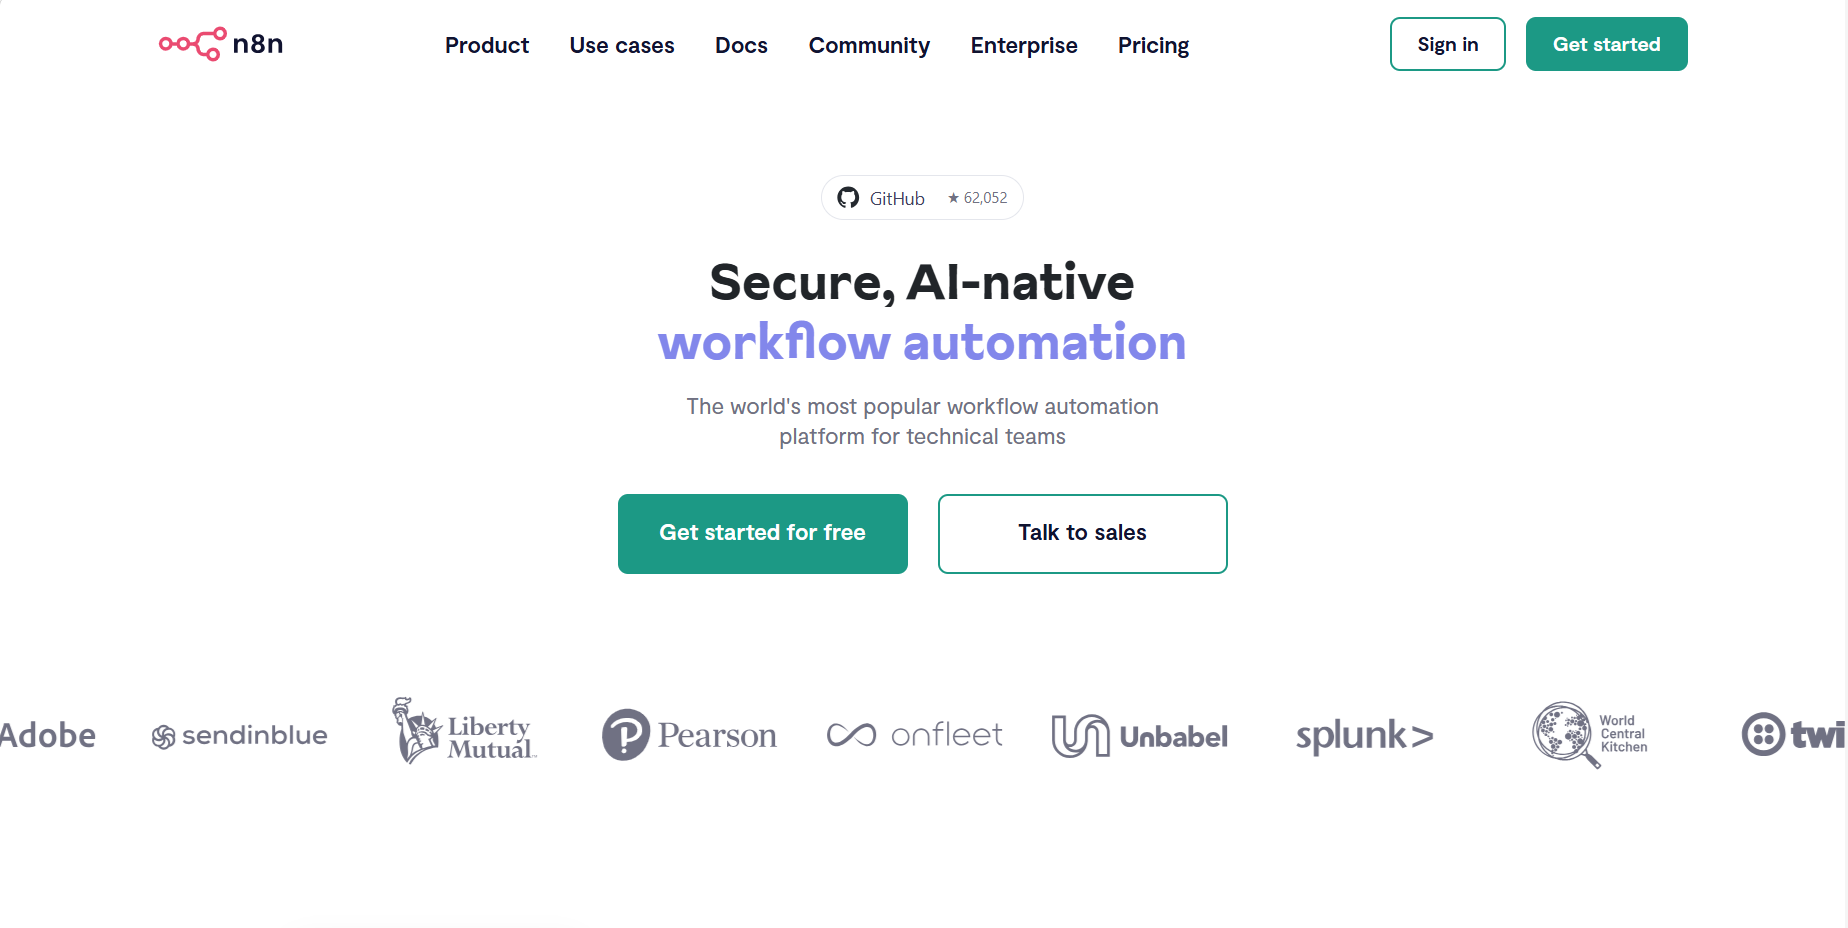
\includegraphics[width=1\linewidth]{images/n8n.png}
    \caption{Trang chủ n8n}
\end{figure}

Tưởng tượng bạn có một công cụ mà bạn có thể "vẽ" các quy trình làm việc phức tạp chỉ bằng vài cú nhấp chuột, kết nối hàng trăm ứng dụng và thậm chí tích hợp trí tuệ nhân tạo để tạo ra những điều kỳ diệu. Để làm được việc đó n8n ra đời - một nền tảng tự động hóa mã nguồn mở, thân thiện với người mới bắt đầu lẫn lập trình viên dày dặn kinh nghiệm. 

$\Rightarrow$ Bạn chỉ cần nghĩ một workflow giúp ích cho cộng đồng hay chính bản thân bạn. Rồi kéo kéo thả thả, n8n sẽ giúp bạn tạo và tự động hóa quy trình đó.

\newpage
Thoạt nghe, điều này có vẻ đơn giản và không ảnh hưởng đến nhiều công việc hằng ngày. Nhưng khi để ý sâu hơn về các công việc ta thường làm hằng ngày theo các biểu đồ swinland, bạn có thấy có rất nhiều công việ nhỏ lặp đi lặp lại: Sáng dạy việc đầu tiên là mở mắt, ngáp nhẹ cái, gấp chăn, mở điện thoại lên check tin nhắn, vươn vai, đánh răng rửa mặt, ăn sáng rồi đi làm. Nếu chúng ta có thể tìm cách để các công việc này có thể tự động tối ưu thì lợi ích mang lại quả không nhỏ.

Bạn cũng sẽ tiết kiệm được thời gian chuyển đổi giữa các công việc. Nhiều nghiên cứu đã chỉ ra rằng việc thay đổi ngữ cảnh giữa các nhiệm vụ có thể tốn khoảng 20 phút để lấy lại sự tập trung. Nếu bạn loại bỏ một nhiệm vụ, bạn cũng loại bỏ luôn khoảng thời gian chuyển đổi đó. Ngoài ra, còn có thời gian bị lãng phí khi chờ đợi một quy trình hoàn thành.

Ví dụ, nếu bạn phải điền một biểu mẫu trực tuyến với thông tin như tên người dùng và mật khẩu, sau đó chờ email xác nhận, thì thời gian chờ đó đã bị lãng phí. Thay vào đó, nếu bạn cấu hình n8n để gửi dữ liệu qua API, bạn sẽ không chỉ loại bỏ việc nhập thủ công mà còn không cần chờ email xác nhận. n8n có thể tự động thực hiện toàn bộ quy trình này chỉ trong một phần nhỏ thời gian bạn cần để nhập liệu và chờ đợi. Giả sử bạn cần thực hiện tác vụ này 80 lần một ngày, chắc chắn bạn sẽ muốn tìm cách tự động hóa nó, đúng không nào :) ?



\section{Lịch sử phát triển}

Trở về năm 2019 – giữa thời kỳ bùng nổ của các nền tảng tự động hóa như Zapier và IFTTT – Jan Oberhauser, một lập trình viên người Đức, nhận ra một khoảng trống lớn mà các công cụ kia không thể lấp đầy. Chúng mạnh mẽ, dễ dùng, nhưng lại giới hạn: giới hạn trong khả năng tùy biến, trong quyền kiểm soát dữ liệu, và trong sự tự do mà những người làm công nghệ thực sự cần.

Jan không chỉ muốn một công cụ kéo-thả đơn giản để “kết nối A với B”. Anh muốn tạo ra một nền tảng mà mọi người – từ lập trình viên đến doanh nhân – đều có thể tự tay xây dựng những hệ thống tự động hóa phức tạp, tích hợp AI, tự viết hàm xử lý riêng, và đặc biệt: được toàn quyền kiểm soát dữ liệu của mình.

$\Rightarrow$ Thế là n8n ra đời.

\newpage

\begin{figure}[htbp]
    \centering
    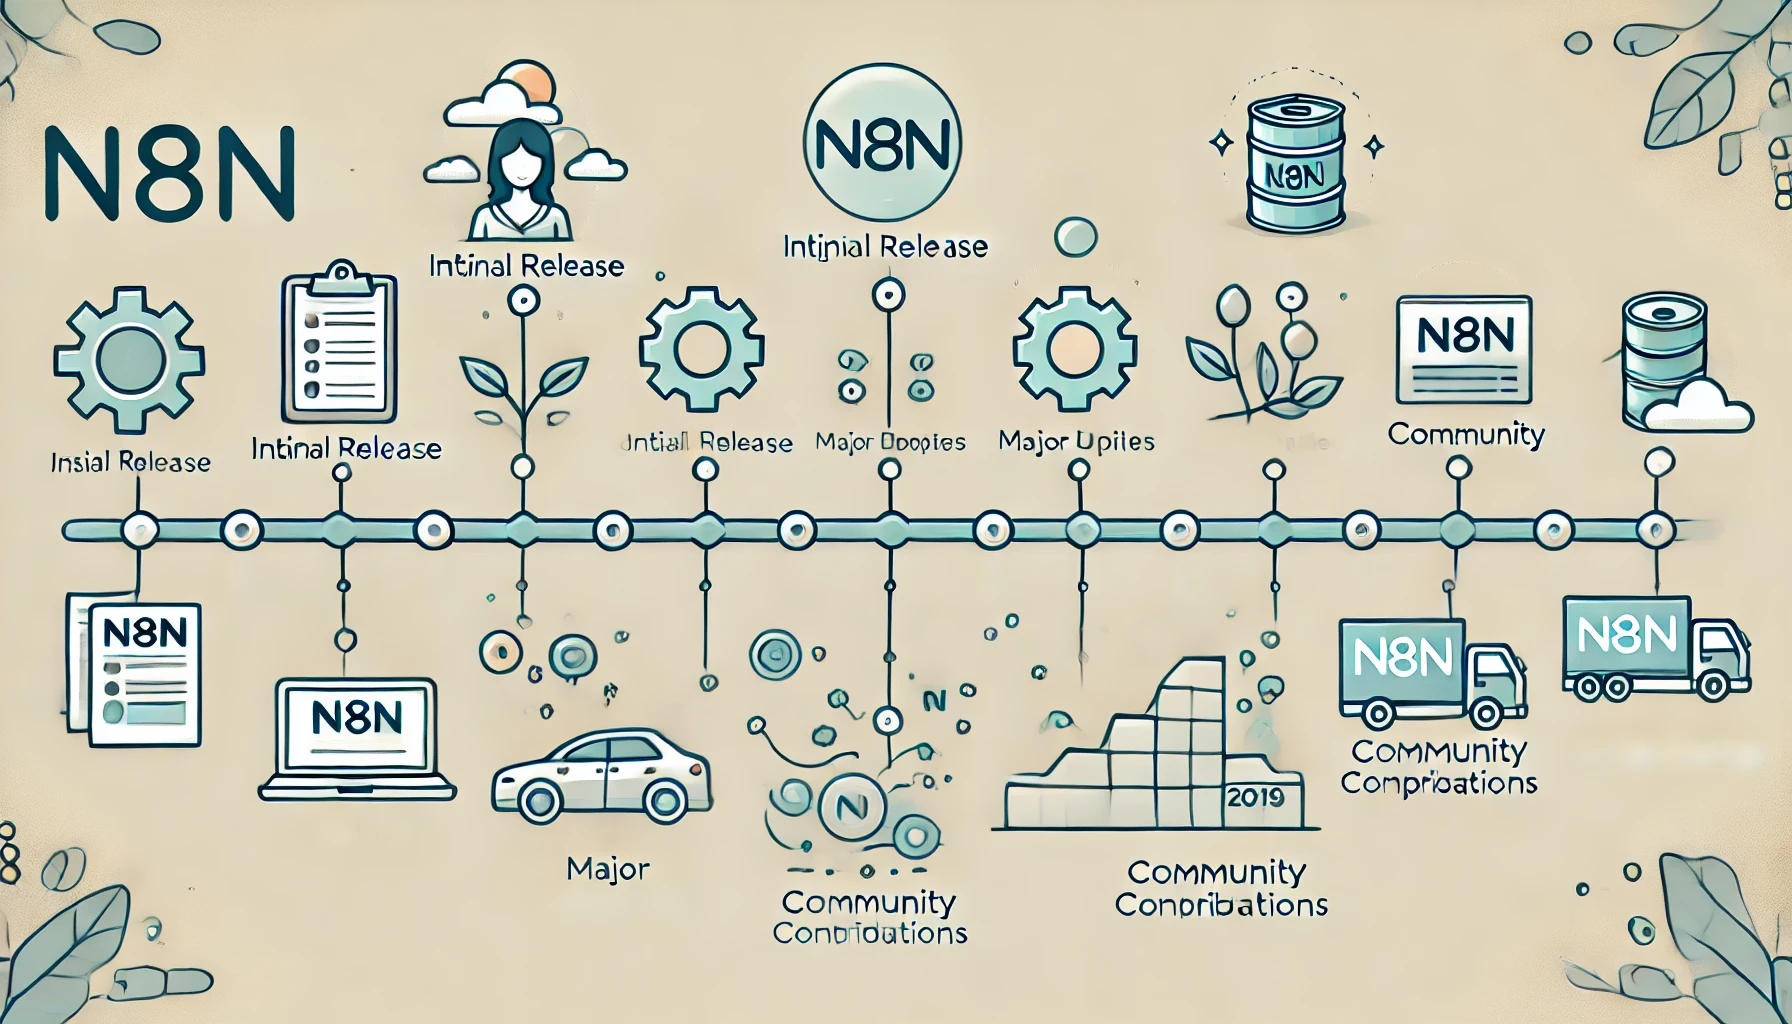
\includegraphics[width=1\linewidth]{images/history.png}
\end{figure}

\textbf{Sự khác biệt đến từ tư duy mở}

Ngay từ khi hình thành, n8n đã chọn cho mình một con đường rất riêng: mã nguồn mở, hoàn toàn có thể tự lưu trữ, và không ràng buộc người dùng vào một hệ sinh thái đóng.

Điều đó có nghĩa là gì? Có nghĩa là bạn có thể triển khai n8n trên bất kỳ máy chủ nào – từ chiếc Raspberry Pi nhỏ bé đến một hệ thống cloud khổng lồ. Bạn có thể tích hợp hơn 200 dịch vụ phổ biến, hoặc gọi bất kỳ API nào bạn muốn. Bạn có thể chỉnh sửa logic, viết JavaScript, thêm node tùy biến. Không giới hạn. Không phụ thuộc. Không đánh đổi quyền riêng tư.

$\Rightarrow$ n8n trao cho bạn chìa khóa để điều khiển luồng dữ liệu – theo cách của riêng bạn.

Hãy nhớ lại lần cuối bạn phải thủ công sao chép dữ liệu từ Excel sang email, hay mất hàng giờ kiểm tra thông báo rải rác trên nhiều nền tảng. n8n không chỉ giúp bạn làm những việc đó - nó làm chúng nhanh hơn, thông minh hơn, và thậm chí có thể đưa ra quyết định thay bạn. Đây không chỉ là công cụ tự động hóa, mà là chìa khóa mở ra một cách làm việc mới, nơi công nghệ không thay thế con người, mà nâng tầm khả năng của chúng ta.

$\Rightarrow$ N8N không chỉ giúp bạn làm việc hiệu quả hơn. Nó thay đổi cách bạn suy nghĩ về công việc.
        
\newpage
\section{Low-code và No-code}
Trong suốt hàng thế kỷ qua, phần mềm đã hoàn toàn thay đổi cách chúng ta làm việc và sinh hoạt. Những hệ thống đắt đỏ và cồng kềnh vốn chỉ dành cho khoa học và nghiên cứu giờ đấy đã trở nên phổ biến như xe cộ bên đường, thật chí nó còn dày đặc hơn thế. Giờ đây, chúng ta có thể làm việc với những người cách chúng ta một vòng trái đất một cách dễ dàng như việc trao đổi bài tập với lũ bạn trên đường. 

Những hệ thống này đã thay đổi xã hội hiện đại nhờ khả năng tự động hóa các nhiệm vụ phức tạp cồng kềnh và xử lý dữ liệu một cách nhất quán. Thay vì phải viết thư tay, dán tem, gửi qua bưu điện và người nhận sẽ có nó trong một vài ngày. Nhờ vào hạ tầng công nghệ hiện đại giờ đây việc gửi một bức thư chỉ diễn ra trong vòng một tích tắc.


Để xây dựng các hệ thống như vậy, trước đây bạn phải học một ngôn ngữ lập trình và thực sự làm chủ nó để viết các đoạn mã hệ thống. Việc này đòi hỏi tính kiên trì, học thuật, logic. Chúng mất quá nhiều thời gian và công sức. Một lựa chọn khác khá phổ biến hiện nay là thuê ngoài. Đơn giản nghe vẻ hợp lý nhưng bạn thử nghĩ bạn đi đâu để tìm một kĩ sư phù hợp và bạn có thực sự đủ tiền để trả cho kĩ sư đó. Để giải quyết khó khăn này các ứng dụng lowcode, nocode ra đời như một sự kiện tất yếu.

\begin{figure}[htbp]
    \centering
    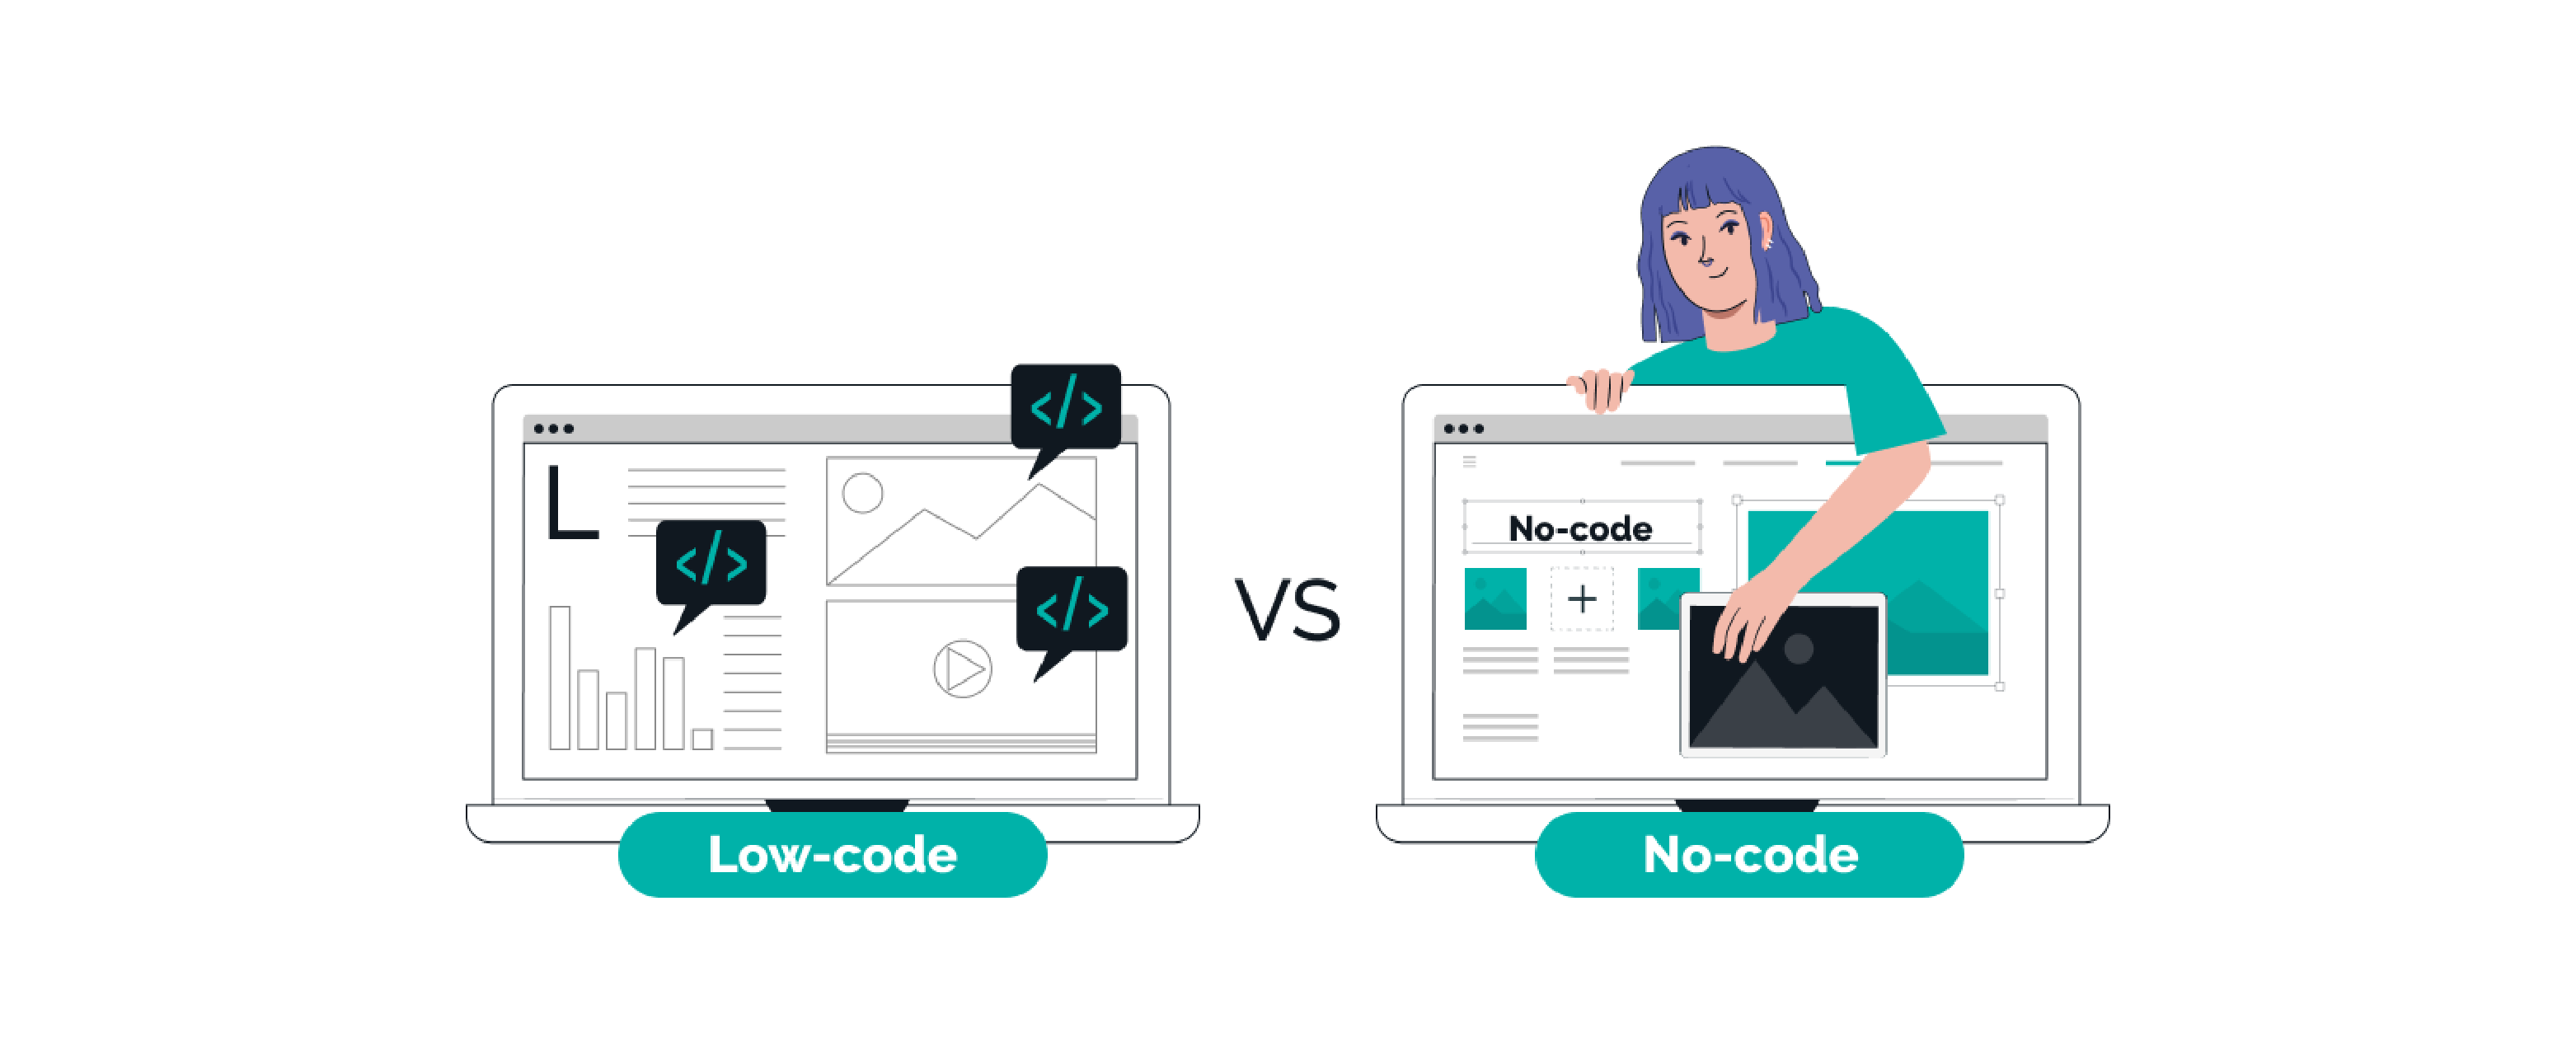
\includegraphics[width=1\linewidth]{Chap1-7/cover-Low-Code.pdf}
\end{figure}

Khi muốn tự động hóa quy trình, chúng ta sẽ nghĩ ngay đến việc dùng phần mềm. Nhưng để có phần mềm, thường phải viết code – mà code thì rắc rối, phức tạp, đòi hỏi các lập trình viên phải vắt óc suy nghĩ, gõ bàn phím đến mức "đầu bù tóc rối", thậm chí có nguy cơ hói sớm :):)

Việc này tạo ra rào cản lớn cho tự động hóa:
\begin{itemize}
    \item Cần nhiều thời gian, công sức để học và viết code.

    \item Khi quy trình thay đổi, lại phải chỉnh sửa code, tốn kém và mất thời gian.

    \item Doanh nghiệp lớn có đội ngũ kỹ thuật thì không sao, nhưng doanh nghiệp nhỏ sẽ phải thuê ngoài, chi phí không hề nhỏ.
\end{itemize}

\textbf{Low - code vs No - code}
\begin{itemize}
    \item \textbf{Low - code:} Cắt giảm đáng kể lượng code. Thay vì phải viết từ A đến Z, giờ đây chỉ cần kéo thả là chính, chỉ khi cần tính năng đặc biệt mới phải viết một chút code.

    \item \textbf{No - code:} Hoàn toàn không cần code, chỉ kéo thả là có thể tạo ra phần mềm.
\end{itemize}

\textbf{Tranh cãi xung quanh "no code"}

Với nhiều kỹ sư kỳ cựu, các công cụ no-code từng bị xem nhẹ như một món vũ khí… thiếu sát thương – dễ dùng, nhưng không đủ lực để giải quyết bài toán phức tạp. Sử dụng no-code đôi khi bị ngầm hiểu là dấu hiệu của một kỹ sư "non tay". Chẳng hạn, các công cụ ETL dạng kéo-thả như Talend – một nhóm yêu thích vì dễ dùng, nhóm khác lại chê vì khó mở rộng và thiếu linh hoạt trong xử lý hàng loạt.

Quan điểm này từng có lý, nhất là khi no-code còn sơ khai. Nhưng vài năm trở lại đây, ranh giới giữa no-code và code đã mờ dần. Khi các nền tảng no-code ngày càng mạnh mẽ và linh hoạt hơn, giá trị thực tế mà chúng mang lại cho doanh nghiệp không thể xem thường. Không còn là giải pháp "tạm bợ", no - code đang dần trở thành lựa chọn chiến lược.


\textbf{N8N: Vừa Low-code vừa No-code}

N8N là ví dụ điển hình cho làn sóng mới này. Nó không thuần no-code, cũng không ép người dùng phải code như một lập trình viên chuyên nghiệp. Với các workflow đơn giản, bạn có thể kéo – thả mà không cần viết dòng nào. Nhưng khi cần tự do hơn, bạn hoàn toàn có thể nhúng vài đoạn mã nhỏ – dễ hiểu, dễ sửa, và không hề phức tạp như xây một hệ thống từ con số 0.

$\Rightarrow$ Nói cách khác, N8N giúp bạn tự động hóa nhanh chóng mà không cần là dân lập trình chuyên nghiệp.




\newpage
\section{Tại sao nên học n8n?}

% Từ thời chinh chiến nơi giảng đường đại học, hằng ngày lòa mắt với từng con số phép tính vi phân, tích chập. Học mãi chẳng vào vì chúng quá là phức tạp. Tư duy mãi cũng ko biết làm, thi mãi điểm cũng chả cao, rồi chán rồi nản. Ở đây n8n không thế, nó cực kỳ easy cho người mới bắt đầu ko nhất thiết phải có tí tech tủng trong người mà vẫn tung hoành thiên hạ được. 
Hồi còn “chinh chiến” nơi giảng đường, ngày ngày vật lộn với vi phân, tích chập, những con số như nhảy múa trước mắt. Học mãi không vào, làm mãi chẳng ra, thi xong nhìn điểm mà muốn xỉu. Tưởng chừng như công nghệ hay tự động hóa là thứ gì đó xa vời, chỉ dành cho những người giỏi kỹ thuật.

\begin{figure}[htbp]
    \centering
    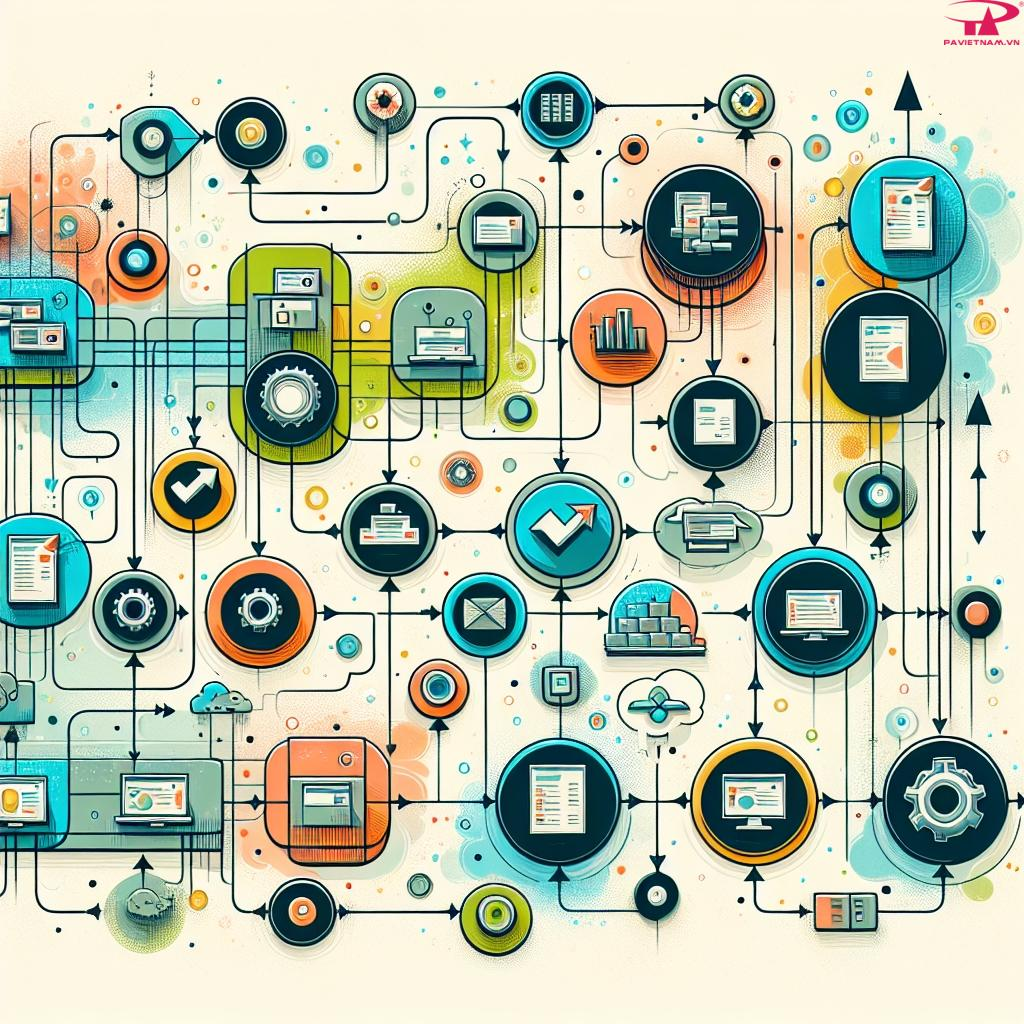
\includegraphics[width=1\linewidth]{images/wf.jpg}
    \caption{Minh họa các node}
\end{figure}

Nhưng rồi mình gặp n8n.

Một nền tảng tự động hóa thân thiện đến không ngờ. Không cần giỏi lập trình, không cần “máu tech”, chỉ cần một chút tò mò và sự kiên nhẫn là đã có thể bắt đầu tạo ra những quy trình tự động giúp cuộc sống và công việc nhẹ nhàng hơn hẳn. Với n8n, bạn có thể “làm điều lớn” mà không cần “kiến thức lớn”.

Học n8n không giống như học code kiểu truyền thống — nó gần giống như chơi lego, ráp từng mảnh nhỏ thành một hệ thống tự động hóa hoàn chỉnh. Và chính cảm giác “tự tay làm được” ấy mới khiến mình mê mẩn n8n đến vậy.

Như tôi nói ở trên ấy, n8n chỉ việc set up rồi chỉ việc tư duy để kéo thả qua các node (node là gì nói sau). Ko phải cầu kỳ như dân dev 

Tự động hóa - Chìa khóa để trở thành doanh nghiệp dựa trên dữ liệu. Quan sát thử bảng sau:

\begin{table}[h]
    \centering
    \renewcommand{\arraystretch}{1.5}
    \begin{tabular}{| m{6cm} | m{6cm} |}
        \hline
        \textbf{Công việc thủ công} & \textbf{Tự động hóa} \\
        \hline
        Lãng phí thời gian & Tính dự đoán cao \\
        \hline
        Lỗi do con người (các nhiệm vụ lặp đi lặp lại có giá trị thấp) & Cải thiện khả năng truy cập dữ liệu - Tăng ROI lên nhiều\\
        \hline
        Yêu cầu nhiều nhân lực & Tăng hiệu suất làm việc của nhân viên \\
        \hline
        Nhân viên ít hạnh phúc và khó giữ chân & Tập trung vào các nhiệm vụ có giá trị cao hơn \\
        \hline
    \end{tabular}
    \caption{So sánh giữa Công việc thủ công và Tự động hóa}
\end{table}

\textbf{Tôi tóm gọn trong 5 lý do sau này:}

\begin{itemize}
    \item Giá rẻ và mã nguồn mở - không tốn phí subscription như Zapier hay Make, phù hợp để học và thử nghiệm
    \item Dễ học với giao diện trực quan - kéo thả node để tạo workflow, không cần code nhiều
    \item Tự do kiểm soát, riêng tư - có thể tự host, quản lý dữ liệu và customize theo ý muốn
    \item Đa năng và mạnh mẽ - tích hợp được nhiều service, chạy được code JavaScript/Python, xây dựng được các workflow phức tạp
    \item Kỹ năng hot - automation đang nổi lên như một xu hướng, biết n8n sẽ tăng giá trị CV và cơ hội nghề nghiệp của bản thân
    \item Hỗ trợ hơn 200 tích hợp sẵn: Kết nối với các dịch vụ phổ biến như Google, Slack, Twitter, v.v.
\end{itemize}

\section{n8n ở đâu trước cơn hót trend Automation}

% Các đối thủ như Zapier, Make là các giải pháp độc quyền, hosting tập trung và tính phí theo subscription

% \begin{itemize}
%     \item Zapier: Hạn chế về tính linh hoạt, chỉ hỗ trợ một số tính năng nhất định, chủ yếu dựa trên các workflows đơn giản.
%     \item n8n: Linh hoạt hơn rất nhiều, hỗ trợ custom code, dễ dàng kết nối API và xử lý các workflows phức tạp.
%     \item Integromat (Make): Tương tự như n8n, nhưng n8n miễn phí mã nguồn mở và có tính năng tùy chỉnh sâu hơn.
% \end{itemize}

Trên thị trường nền tảng tự động hóa, những cái tên như Zapier hay Make từ lâu đã trở thành lựa chọn quen thuộc với người dùng nhờ giao diện thân thiện và khả năng triển khai nhanh. Tuy nhiên, cả hai đều là các nền tảng độc quyền, lưu trữ tập trung trên cloud, và tính phí theo mô hình subscription – điều này có thể khiến doanh nghiệp phải phụ thuộc vào hạ tầng và định giá của bên thứ ba trong suốt quá trình sử dụng.

\begin{itemize}
    \item Zapier – tuy nổi tiếng vì dễ dùng, nhưng lại khá hạn chế về tính linh hoạt. Hầu hết người dùng chỉ có thể sử dụng các bước workflow đơn giản với tập hợp chức năng giới hạn. Zapier không cho phép can thiệp sâu bằng code, khiến việc xử lý các tác vụ phức tạp trở nên khó khăn hoặc không khả thi.

    \item Make – được đánh giá cao hơn Zapier về mức độ tùy chỉnh và khả năng xử lý các quy trình tự động hóa phức tạp. Tuy nhiên, Make vẫn là một nền tảng độc quyền với chi phí sử dụng có thể tăng nhanh khi mở rộng quy mô. Việc triển khai hoàn toàn phụ thuộc vào hệ thống cloud của họ, khiến người dùng không thể kiểm soát hoặc host cục bộ nếu cần.
    \item Khác biệt với hai đối thủ trên, n8n chọn một hướng đi táo bạo: mã nguồn mở, có thể host tại chỗ, miễn phí và cực kỳ linh hoạt. Người dùng không chỉ có thể kéo – thả để xây workflow đơn giản, mà còn dễ dàng nhúng custom code, gọi REST API, xử lý dữ liệu nâng cao và tích hợp với các hệ thống phức tạp. Với n8n, việc mở rộng quy trình hay kiểm soát luồng dữ liệu không còn là điều “bất khả thi” như ở các nền tảng đóng.

\end{itemize}
Thêm vào đó, vì là mã nguồn mở, n8n cho phép người dùng can thiệp vào logic hệ thống, tùy chỉnh sâu theo nhu cầu nội bộ mà không bị ràng buộc bởi giới hạn của nhà cung cấp. Đây là một lợi thế chiến lược với các đội ngũ kỹ thuật muốn tiết kiệm chi phí dài hạn, đồng thời đảm bảo quyền kiểm soát tuyệt đối với hệ thống của mình.




\section{n8n có thể làm được gì?}

n8n là một công cụ hoạt động trên nền tảng web, có thể chạy trên các thiết bị nhỏ gọn và giá rẻ như Raspberry Pi. Nó có thể kết nối với hàng trăm hệ thống khác nhau thông qua các node được thiết kế riêng, cũng như hàng nghìn hệ thống khác thông qua REST API tiêu chuẩn.

n8n không chỉ có khả năng chuyển đổi và xử lý dữ liệu, mà còn có thể thực hiện phân tích dữ liệu để cung cấp những thông tin hữu ích. Vì có thể tích hợp với hầu hết các hệ thống có API, nên khả năng của n8n chỉ bị giới hạn bởi những hệ thống mà nó kết nối.

Ví dụ:
\begin{itemize}
    \item Bạn muốn tạo hình ảnh 3D tự động? Có một API cho việc đó.

    \item Bạn muốn remix nhạc theo màu sắc mà webcam thu thập? Bạn có thể tạo một workflow để làm điều này.
    
    \item Bạn muốn n8n tự động cân đối sổ sách và hiển thị tình hình tài chính theo thời gian thực? Điều đó hoàn toàn có thể.

    \item Nếu có cách để kết nối n8n với một hệ thống, thì n8n có thể kế thừa sức mạnh của hệ thống đó.
\end{itemize}


% Chương 2
\chapter{Cài đặt \& Môi trường làm việc}

% Nếu bạn nghĩ tự động hóa là thứ gì đó phức tạp, đòi hỏi hàng giờ lập trình hay một bộ óc thiên tài, thì chương này sẽ khiến bạn phải nghĩ lại. Với n8n, bạn không cần phải là Tony Stark để xây dựng một Jarvis cá nhân – bạn chỉ cần một chút tò mò và vài phút rảnh rỗi.

Nếu bạn từng nghĩ rằng tự động hóa chỉ dành cho các lập trình viên kỳ cựu, những bộ óc thiên tài hay những người làm việc trong phòng lab của Tony Stark, thì chương này sẽ khiến bạn phải nhìn lại. Sự thật là: với n8n, bạn không cần đến một đội ngũ kỹ sư, không cần phải ngồi gõ hàng trăm dòng mã, và càng không cần phải “nạp não” với những khái niệm lập trình phức tạp. Bạn chỉ cần một chiếc máy tính, một chút tò mò, và một chút thời gian giữa giờ cà phê.

Hãy bắt đầu bằng việc cài đặt n8n. Tôi sẽ dẫn bạn qua hai con đường: dùng phiên bản đám mây để thử ngay lập tức, hoặc tự lưu trữ trên máy tính nếu bạn muốn kiểm soát hoàn toàn. Đừng lo, quá trình này đơn giản đến mức bạn sẽ hoàn thành trước khi tách trà của bạn nguội đi.


\section{Cài đặt trên Windows, macOS, Linux}

\section{Chạy trên Cloud}
Truy cập trang chủ của \href{n8n.io}{n8n.io}, làm theo các hướng dẫn để đăng ký tài khoản, không cần cấu hình server, trả phí định kỳ.

- Điền đầy đủ các thông tin cần thiết, email, username, password, account\_name - domain khi sử dụng N8N. 

$\Rightarrow$ Đăng ký xong có ngay 14 ngày sài free để mọi người trải nghiệm dịch vụ nha. Sau đó cứ theo mức phí ở phần pricing mà trừ tiền nha :))

\section{Cài bằng node trên AWS EC2}

Bạn biết gì không, mỗi tài khoản AWS mới tạo sẽ được miễn phí một số tài nguyên. Mỗi tháng bạn sẽ có 750h free dùng t2.small (1v CPU, 2GB Ram). Vì vậy việc dùng AWS EC2 cx là một lựa chọn khá hợp lý.

Trước tiên bạn hãy khởi tạo một con EC2 t2.micro với 8GB bộ nhớ (EBS được free 30GB/tháng). Sau đó connect tới server đó và chạy các lệnh sau

- Lệnh tải n8n

\begin{lstlisting}
sudo npm install n8n
\end{lstlisting}

- Lệnh tắt mã hóa cookie

\begin{lstlisting}[language=bash]
export N8N_SECURE_COOKIE=false
\end{lstlisting}

- n8n thường chạy trong Terminal, nhưng nếu bạn thoát Terminal hoặc khởi động lại máy tính, n8n sẽ ngừng hoạt động. Để giải quyết vấn đề này, chúng ta có thể sử dụng một ứng dụng có tên PM2 để chạy n8n như một dịch vụ kể cả có tắt terminal thì nó vẫn hoạt động. 

\begin{lstlisting}[language=bash]
sudo npm install -g pm2
\end{lstlisting}

- Lệnh chạy n8n:
\begin{lstlisting}[language=bash]
pm2 start n8n --name n8n
\end{lstlisting}

- Lệnh dừng n8n:
\begin{lstlisting}[language=bash]
pm2 stop n8n
\end{lstlisting}

Truy cập giao diện web thông qua trình duyệt (thường là http://localhost:5678 hoặc http://ip:5678).



\subsection{Cài bằng Docker}
Oke nếu pro ko có Cloud, không sao bạn hoàn toàn có thể cài trên máy tính cá nhân. Và tất nhiên để cho gọn thì chúng ta hãy nghĩ đến container

- Tạo file docker-compose.yml mẫu:
\begin{lstlisting}
services:
  n8n:
    image: n8nio/n8n
    restart: unless-stopped
    ports:
      - "5678:5678"
    environment:
      - N8N_BASIC_AUTH_ACTIVE=true
      - N8N_BASIC_AUTH_USER=admin
      - N8N_BASIC_AUTH_PASSWORD=pass
      - N8N_HOST=localhost
      - N8N_PORT=5678
      - N8N_PROTOCOL=http
      - N8N_SECURE_COOKIE=false
    volumes:
      - n8n_data:/home/node/.n8n

volumes:
  n8n_data:
\end{lstlisting}

- Khởi động docker: 

\begin{lstlisting}
    docker-compose up -d
\end{lstlisting}

Do là dùng VPS nên có thể dung NGROK để cấp domain cho ip hiện tại. Do ip thì khó auth với các dịch vụ khác như facebook, google hơi khó.

\section{Cách cứu vãn trong trường hợp quên password n8n}

Kiểu gì cũng có mấy ông bà nào đó lập cái tài khoản xong quên mất. Dùng cloud thì quên mật khẩu dễ dàng. Còn nếu bạn dùng self-host thì sao :))

$\rightarrow$ Dùng CLI 

\begin{enumerate}
    \item Đối với cài bằng node chỉ việc mở terminal lên và chạy lệnh

\begin{lstlisting}[language = Bash]
n8n user-management:reset
\end{lstlisting}

Sau đó khởi động lại n8n là được

    \item Đối với docker

\begin{itemize}
    \item[-] Xem ID của container chứa n8n
\begin{lstlisting}
docker ps
\end{lstlisting}

\begin{lstlisting}
huyvv@server:~$ docker ps
CONTAINER ID   IMAGE       COMMAND   CREATED      STATUS      PORTS               NAMES
f3b82a9435e5 n8nio/n8n "tini -- /docker-entrypoint.sh ..." 3 days ago Up 3 days 0.0.0.0:5678->5678/tcp, [::]:5678->5678/tcp n8n-1
\end{lstlisting}


$\rightarrow$ f3b82a9435e5 là ID của container chứa n8n

\item[-] Truy cập vào container đó
\begin{lstlisting}
docker exec -it f3b82a9435e5 /bin/sh
\end{lstlisting}

\item[-] Chạy lệnh reset tài khoản
\begin{lstlisting}
n8n user-management:reset
\end{lstlisting}
\end{itemize}
\item[-] Tắt và khởi động lại container
\begin{lstlisting}
docker compose down
docker compose up -d
\end{lstlisting}
\end{enumerate}






\newpage

\section{Tổng quan giao diện n8n}

Sau khi cài đặt thành công đây là giao diện ban đầu:

\begin{figure}[htbp]
    \centering
    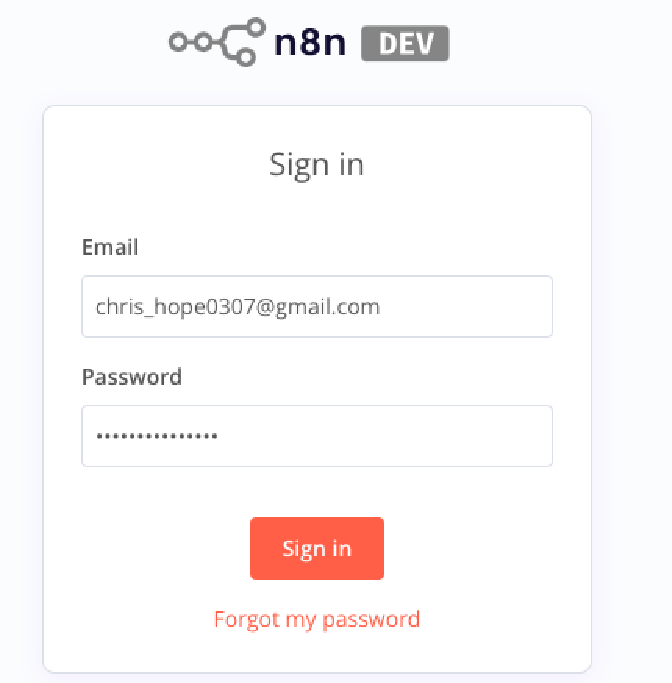
\includegraphics[width=0.8\linewidth]{Chap1-7/login.pdf}
    \caption{Giao diện đăng nhập}
\end{figure}

Editor UI trong n8n là một giao diện trực quan giúp bạn dễ dàng tạo quy trình tự động hóa bằng cách kết nối các node. Cách tiếp cận này lấy cảm hứng từ ngành công nghiệp phim ảnh và truyền hình, nơi mà nhiều công cụ sử dụng hệ thống node-based để xử lý dữ liệu một cách trực quan.

Nhìn lên trên bên trái, bạn sẽ thấy một biểu tượng >, nhấn vào đó để mở rộng menu chính của n8n.

Trước khi đi sâu vào từng tính năng, chúng ta sẽ làm quen với giao diện tổng thể để có thể dễ dàng điều hướng và thao tác. Khi đã thành thạo, bạn sẽ nhanh chóng xây dựng được những quy trình tự động hóa mạnh mẽ mà không cần viết code phức tạp.

Cùng xem menu này có những gì
\begin{itemize}
    \item New: Tạo một workflow mới.

    \item Open: Mở một workflow đã có sẵn.

    \item Save: Lưu thay đổi vào workflow hiện tại.

    \item Save As: Lưu workflow hiện tại với một tên mới.

    \item Rename: Đổi tên workflow.

    \item Delete: Xóa workflow hiện tại.

    \item Download: Tải xuống workflow dưới dạng file JSON.

    \item Import from URL: Nhập workflow từ một URL.

    \item Import from File: Nhập workflow từ một file JSON.

    \item Settings: Cấu hình cài đặt cho workflow hiện tại.
\end{itemize}

\textit{Lưu ý: Đừng quên \textbf{SAVE} lại workflow nếu không công sức brainstorm của pro sẽ bay màu đó :)).}

\textbf{Menu Credentials}

Menu này có hai tùy chọn:
\begin{itemize}
    \item New: Tạo một credential mới.

    \item Open: Mở một credential đã có sẵn.
\end{itemize}

n8n cho phép bạn kết nối với nhiều ứng dụng, dịch vụ và API khác nhau. Nhiều ứng dụng yêu cầu credentials để xác thực quyền truy cập. n8n hỗ trợ mã hóa và lưu trữ các credentials này trong cơ sở dữ liệu, giúp bạn có thể sử dụng lại dễ dàng khi tạo workflows mới.

\textbf{Tab Executions}

Tab này mở một cửa sổ (modal) hiển thị danh sách các lần thực thi của workflows. Bạn cũng có thể lọc executions theo tên và trạng thái.
\section{Nguyên tắc làm việc với n8n}

\begin{itemize}
    \item Hiểu rõ luồng làm việc: Dữ liệu đi từ đâu đến đâu, nó sẽ làm gì trong cái workflow đấy cũng như logic của nó. Workflow phải tối ưu ngắn hiệu quả. Đảm bảo tính nhất quản của dữ liệu trong suốt quy trình. Tránh các bước trung gian không cần thiết để giảm thiểu độ trễ và tài nguyên hệ thống. 
    \item Sử dụng trigger đúng cách: đặt lịch để workflow chạy, nhận dữ liệu trả về từ API, trigger từ các ứng dụng bên ngoài 
    \item Tận dụng các node trước để tối ưu workflow
    \item Kết hợp các nguồn API, webhook bên ngoài để mở rộng workflow 
    \item Quản lý lỗi hiệu quả. Báo lỗi khi workflow xảy ra sự cố. Triển khai node Error Trigger để phát hiện và xử lý các lỗi runtime
\end{itemize}

\newpage
\section{Tối ưu workflow}
\begin{figure}[htbp]
    \centering
    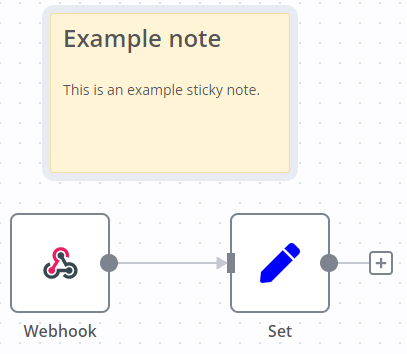
\includegraphics[width=0.8\linewidth]{Chap1-7/sticky-note.png}
    \caption{Sticky note}
\end{figure}

Để tránh trường hợp mà tạo xong workflow méo hiểu mình vừa kéo thả cái gì thì mình nghĩ mọi người nên chú ý các điều sau:
\begin{itemize}
    \item Thiết kế workflow càng dễ càng tốt
    \item Thêm note giải thích chi tiết (Shift + S)
    \item Làm đến đâu giải thích đến đấy
\end{itemize}


\section{Cách import, export worflow}
Tính năng này sinh ra nhằm mục tải worflow của bạn dưới dạng json và backup nó vào trong máy tính local hoặc push lên github để lưu trữ. Sau nay khi cần restore lại thì bạn chỉ cần upload lại 

\begin{itemize}
    \item Nhấn vào nút ba chấm trên cùng góc trái sau đó chọn "\textbf{Download}"
    \item Tương tự chọn "\textbf{Import from file or url} để import lại workflow đã lưu 
\end{itemize}

% Chương 3 
\chapter{Hiểu về Node - Đơn vị cơ bản của n8n}

\begin{figure}[htbp]
    \centering
    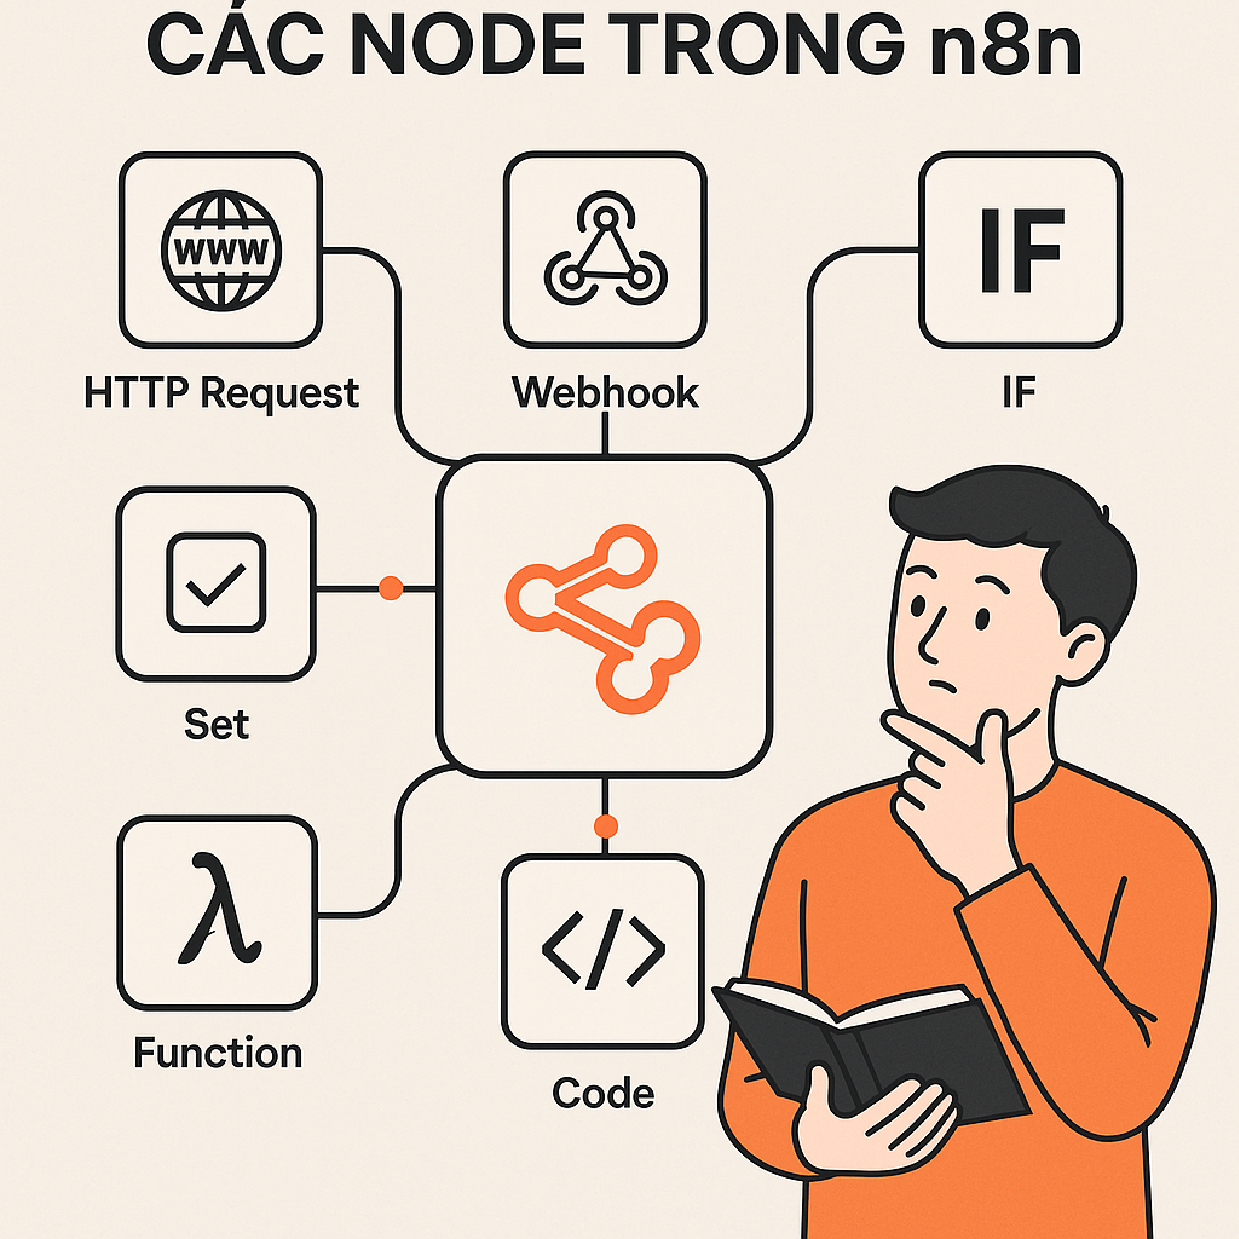
\includegraphics[width=0.96\linewidth]{Chap1-7/node-mh.pdf}
\end{figure}



Tưởng tượng này, bạn đang đứng giữa một công trường rộng lớn, nơi một ngôi nhà đang bắt đầu được dựng lên từ những viên gạch đầu tiên. Xung quanh bạn là tiếng búa, tiếng cưa, những thanh sắt đan xen vào nhau, và những người thợ đang cần mẫn làm việc. Lúc này, có thể bạn chưa thấy gì ngoài bê tông, thép, và bụi bặm – chưa có phòng khách ấm cúng, chưa có ánh đèn vàng hay chiếc ghế sofa yêu thích. Nhưng chính trong sự ngổn ngang ấy, nền móng của một tổ ấm đang dần hình thành.

Người chủ của ngôi nhà có thể đã tưởng tượng ra đủ điều – màu sơn tường, rèm cửa, cách bài trí từng góc nhỏ, thậm chí là cảm giác êm ái của đôi chân trần trên thảm phòng ngủ. Họ háo hức với những chi tiết hoàn mỹ, và có lẽ trong thâm tâm, họ mong có thể bỏ qua giai đoạn "lấm lem" của công trình, để bước thẳng vào phần thú vị nhất: trang trí và tận hưởng. Nhưng ai cũng hiểu rằng, nếu thiếu đi phần nền móng vững chắc, nếu không có những thanh xà ngang được liên kết chuẩn xác, thì chẳng có ngôi nhà nào đủ kiên cố để trường tồn. Những điều đẹp đẽ bên ngoài chỉ có thể toả sáng khi phần khung bên trong được xây dựng cẩn thận, tỉ mỉ.

Việc học lập trình, hay nói cụ thể hơn là học cách xây dựng quy trình tự động hoá trong n8n, cũng giống như vậy. Trong thế giới no-code, bạn không cần phải thông thạo những dòng code rối rắm hay hiểu sâu về các thuật toán phức tạp. Bạn không cần phải là một kỹ sư phần mềm lão luyện. Tuy nhiên, điều đó không có nghĩa là bạn có thể bỏ qua phần “nền móng”. Và trong n8n, các node chính là những viên gạch, là cột trụ, là hệ thống xương sống giúp mọi quy trình hoạt động trơn tru và hiệu quả.

Mỗi node trong n8n đóng vai trò như một công nhân trong đội xây dựng – có node chuyên kéo dữ liệu về, có node chịu trách nhiệm xử lý thông tin, có node phân nhánh điều kiện, và có node đảm nhận việc gửi kết quả đi. Khi bạn hiểu rõ vai trò và cách phối hợp giữa các node, bạn sẽ giống như một kiến trúc sư lành nghề, biết cách chọn vật liệu, sắp xếp không gian và tối ưu từng chi tiết nhỏ nhất. Ngược lại, nếu bạn chỉ kéo-thả mà không thật sự hiểu cách dữ liệu luân chuyển qua từng node, bạn đang xây một ngôi nhà chỉ để “đẹp bề ngoài” – và nó có thể đổ sụp bất cứ lúc nào khi quy trình phức tạp hơn, hoặc khi cần thay đổi điều gì đó.
\newpage

\section{Giao diện người dùng}

\begin{figure}[htbp]
    \centering
    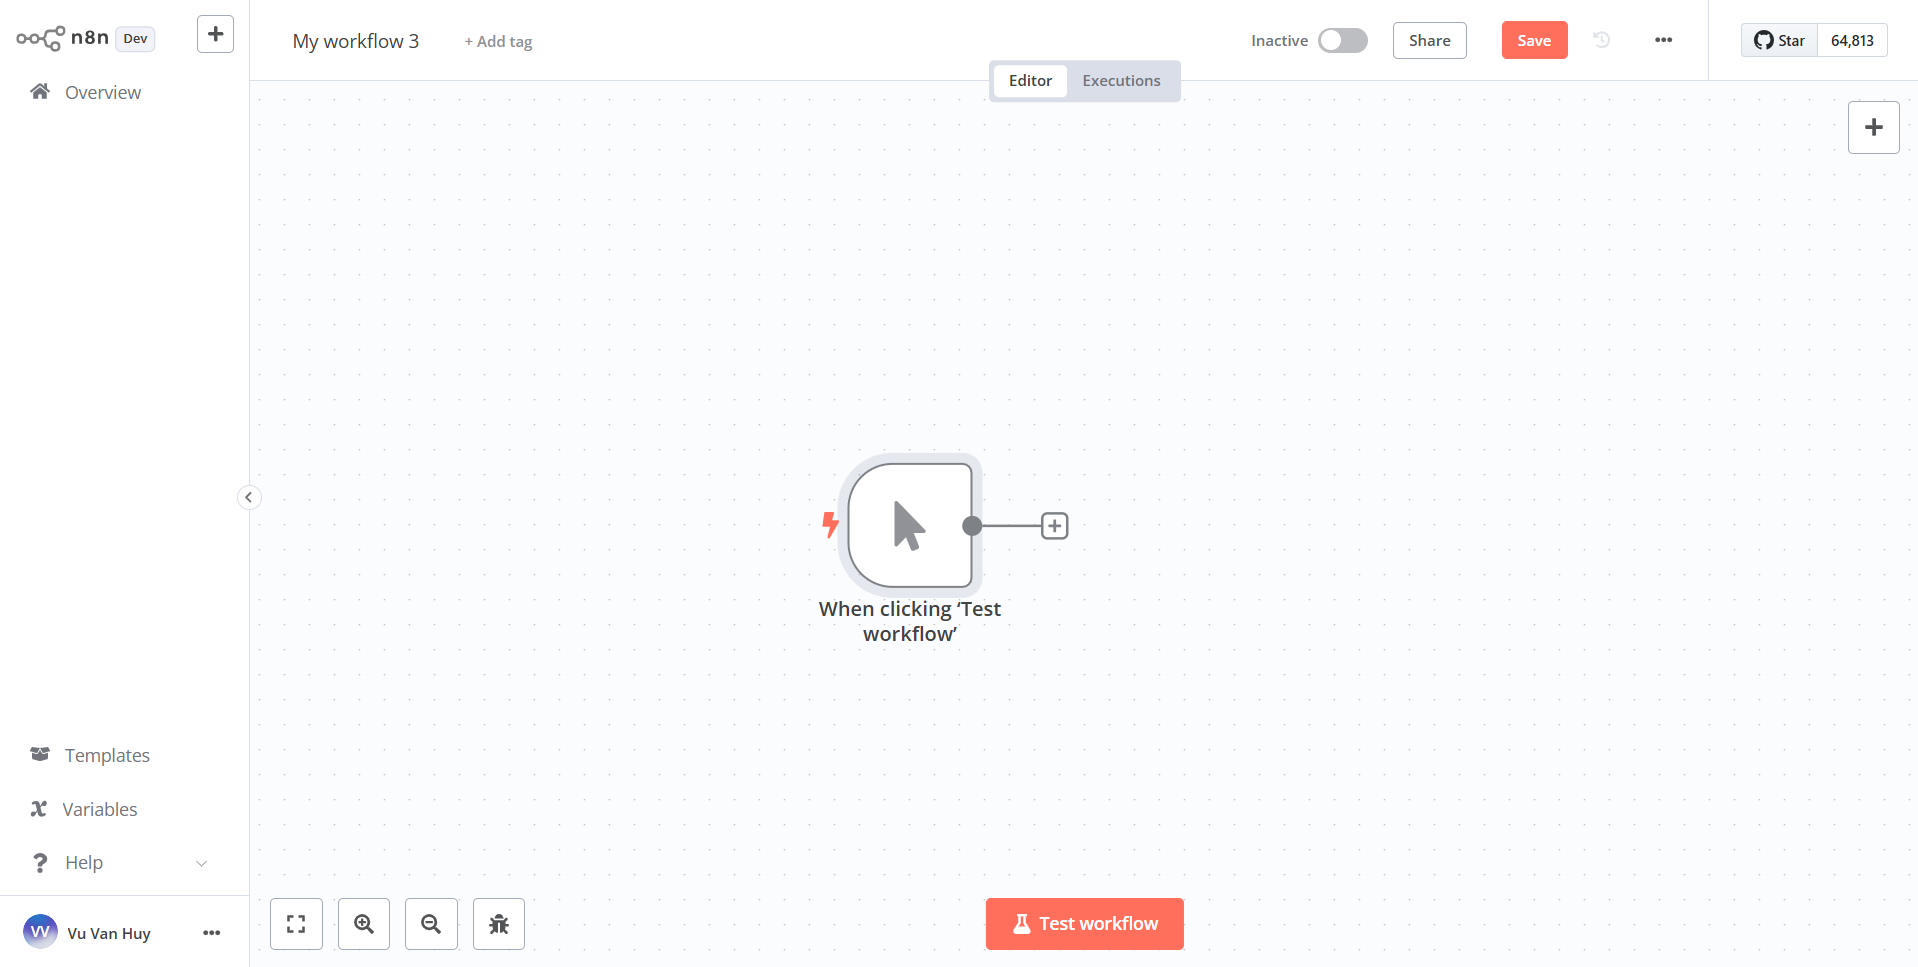
\includegraphics[width=1\linewidth]{Chap1-7/giaodien.png}
    \caption{Giao diện workflow ban đầu}
\end{figure}


Trong n8n, cấu trúc của một workflow bao gồm ba thành phần chính: Input, Output, và Trigger Node. Dưới đây là mô tả chi tiết về từng thành phần này:

\begin{itemize}
    \item Dashboard: Màn hình chính hiển thị danh sách các workflow, trạng thái của từng quy trình, log và các thông báo lỗi.
    \item Thanh Menu: Các mục điều hướng chính như  “Workflows”, “Executions”, “Credentials”, và “Settings”.
    \item Editor Workflow: Khu vực trung tâm dùng để kéo thả, sắp xếp và cấu hình các node.
\end{itemize}

    
Hướng dẫn điều hướng:
\begin{itemize}
    \item Thanh công cụ: Sử dụng các nút zoom, undo/redo và grid để dễ dàng quản lý các node trong workflow.
    \item Tìm kiếm và lọc: Hỗ trợ tìm kiếm workflow theo tên, trạng thái hay theo các từ khóa đã cấu hình.
\end{itemize}

\section{Ngôn ngữ của n8n}
Ngay từ nhỏ, tôi thích chu du khắp nơi, thích đi đây đi đó tìm kiếm những điều mới lạ về các sứ sở ngoài kia. Tôi rất thích và đam mê vẻ hào nhoáng của các đất nước nổi tiếng với nền văn hóa du lịch của họ. Bất lợi thay tôi không thể trải nghiệm toàn bộ nền văn hóa này do tôi chỉ biết và sõi duy nhất một ngôn ngữ là tiếng mẹ đẻ. Việc này dẫn đến việc tôi thường xuyên hiểu sai nghĩa khi bất chợt tôi đọc một cái hay ho nào đó. 

n8n cũng có một ngôn ngữ riêng để các node giao tiếp với nhau. Ngôn ngữ này là JSON, một dạng key - value đơn giản dễ biên dịch cho cả người và máy, là một chuẩn để mô tả thông tin object phổ biến trong tất cả các phần mềm. Nhờ loại ngôn ngữ này chúng ta có thể dễ dàng truyền tải dữ liệu và văn bản dạng nhị phân. Các node đều có input và output dạng JSON. Chúng ta sẽ tìm hiểu kĩ loại ngôn ngữ này để dùng "Expression" để truy suất thông tin JSON. Vì vậy việc nắm vứng các sử dụng JSON là hết sức cần thiết. Và cuốn sách này sẽ nhắc tới rất nhiều ngôn ngữ này. 


\section{Node}

Trong n8n, nodes là các thành phần cơ bản và quan trọng nhất của mỗi workflow. Mỗi node đại diện cho một hành động, một dịch vụ, hoặc một chức năng cụ thể mà bạn muốn thực hiện. Có thể hình dung nodes như các khối xây dựng của quy trình tự động hóa của bạn.

\begin{figure}[htbp]
    \centering
    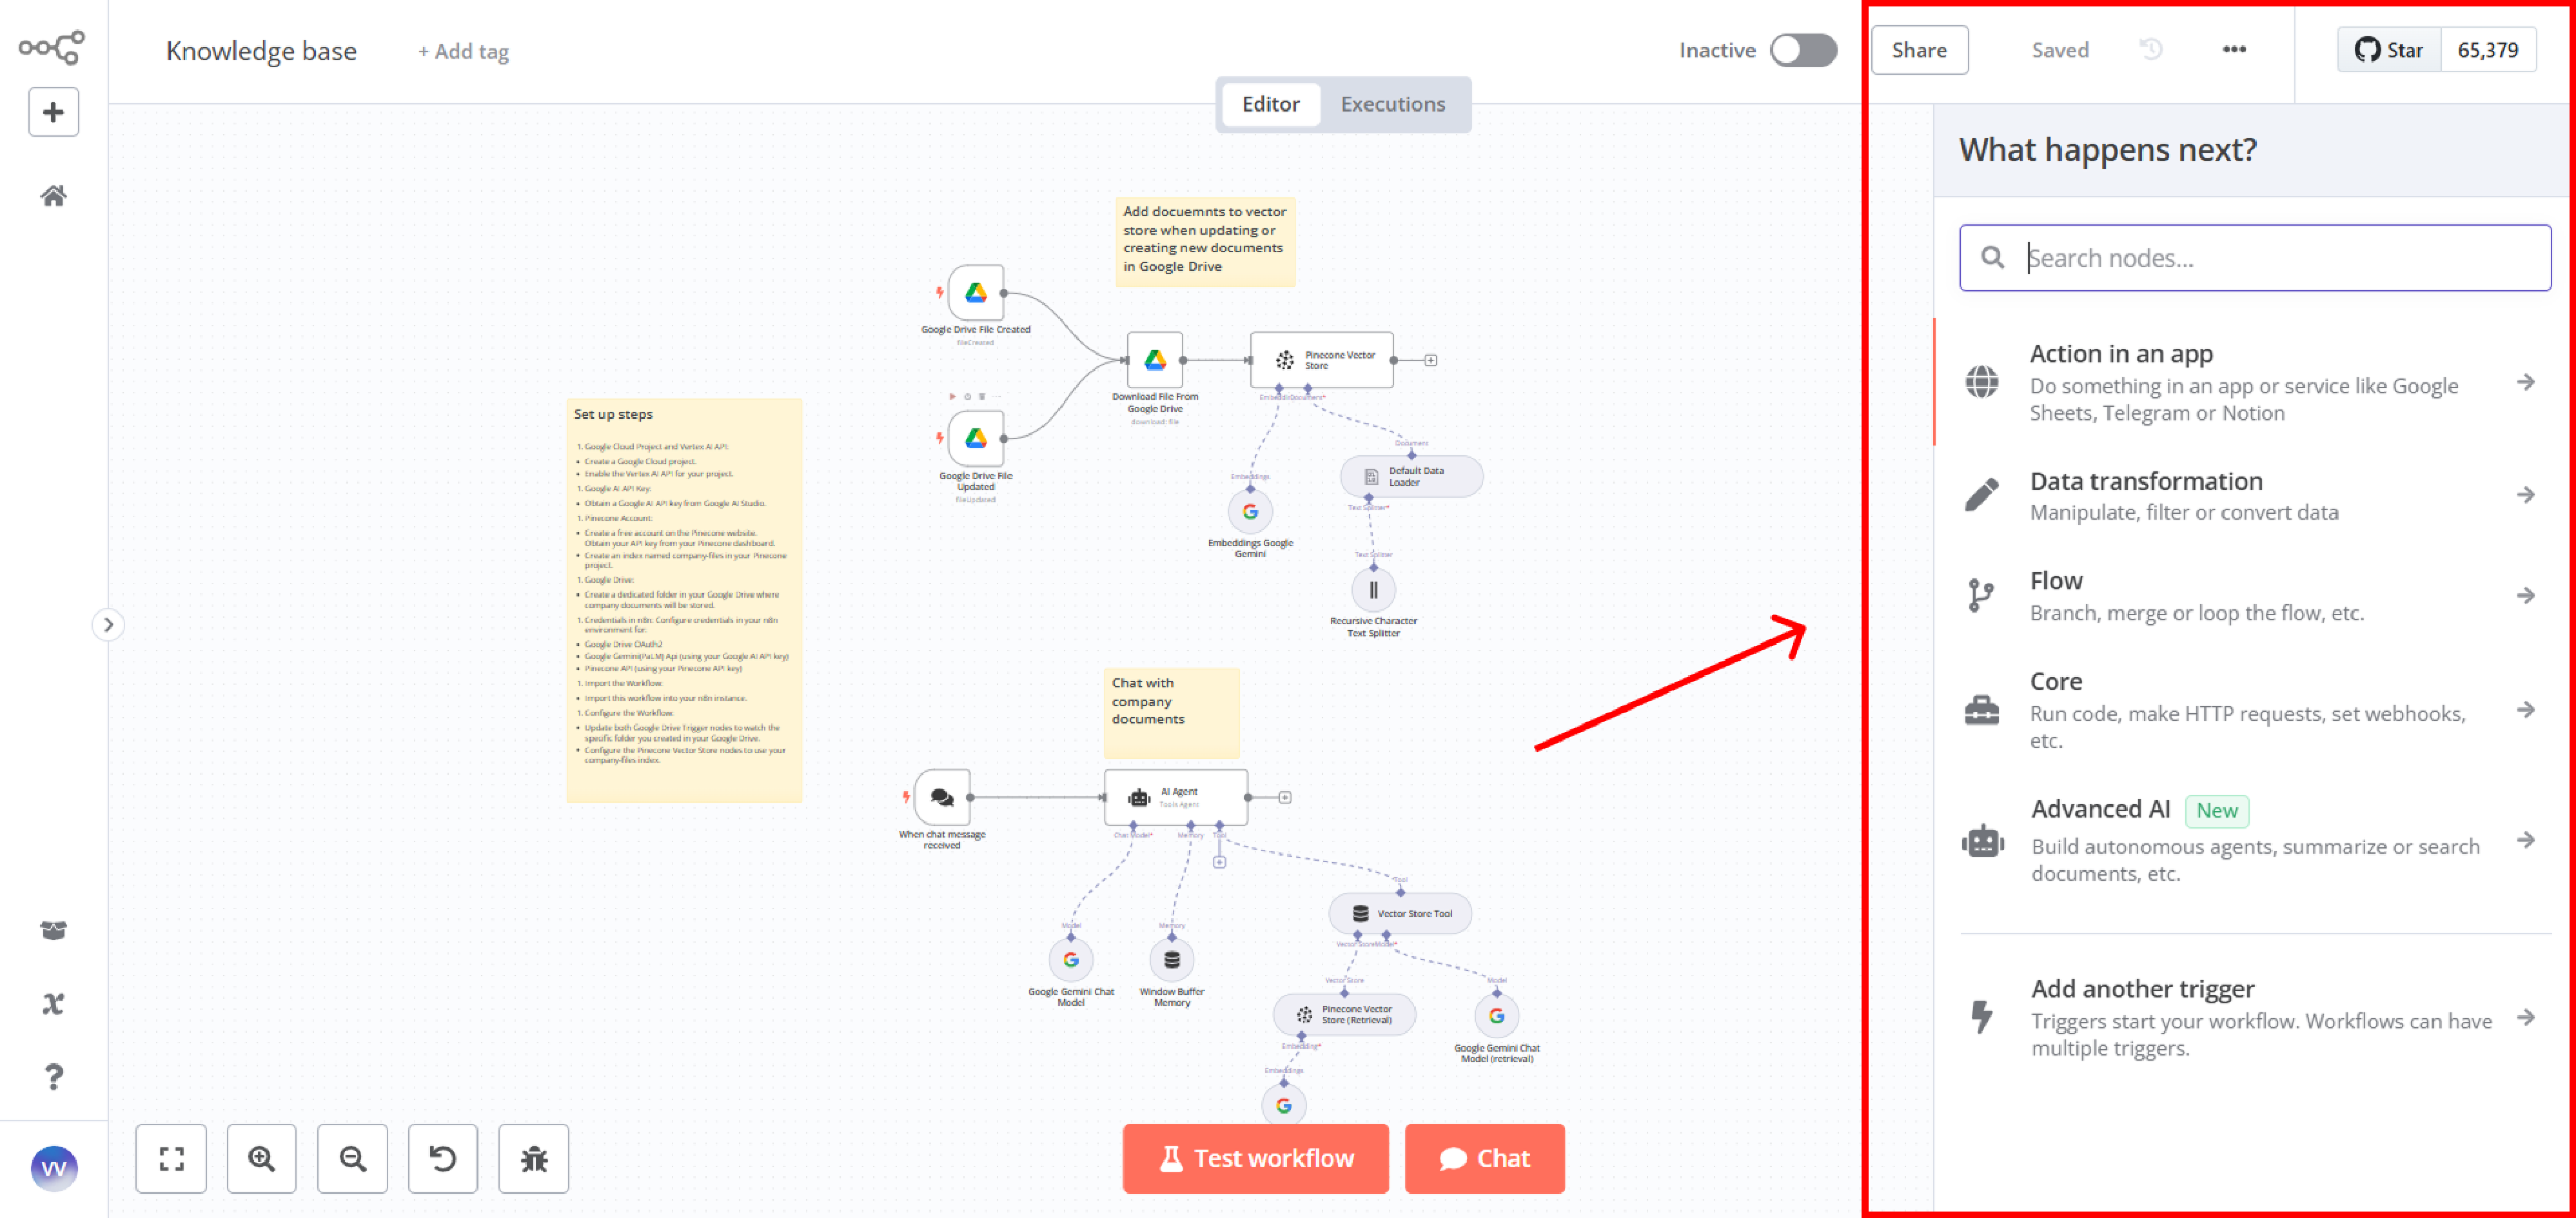
\includegraphics[width=1\linewidth]{Chap1-7/node.pdf}
    \caption{Các option chọn node}
\end{figure}

\newpage

\subsection{Chức năng chính của nodes}

\begin{figure}[htbp]
    \centering
    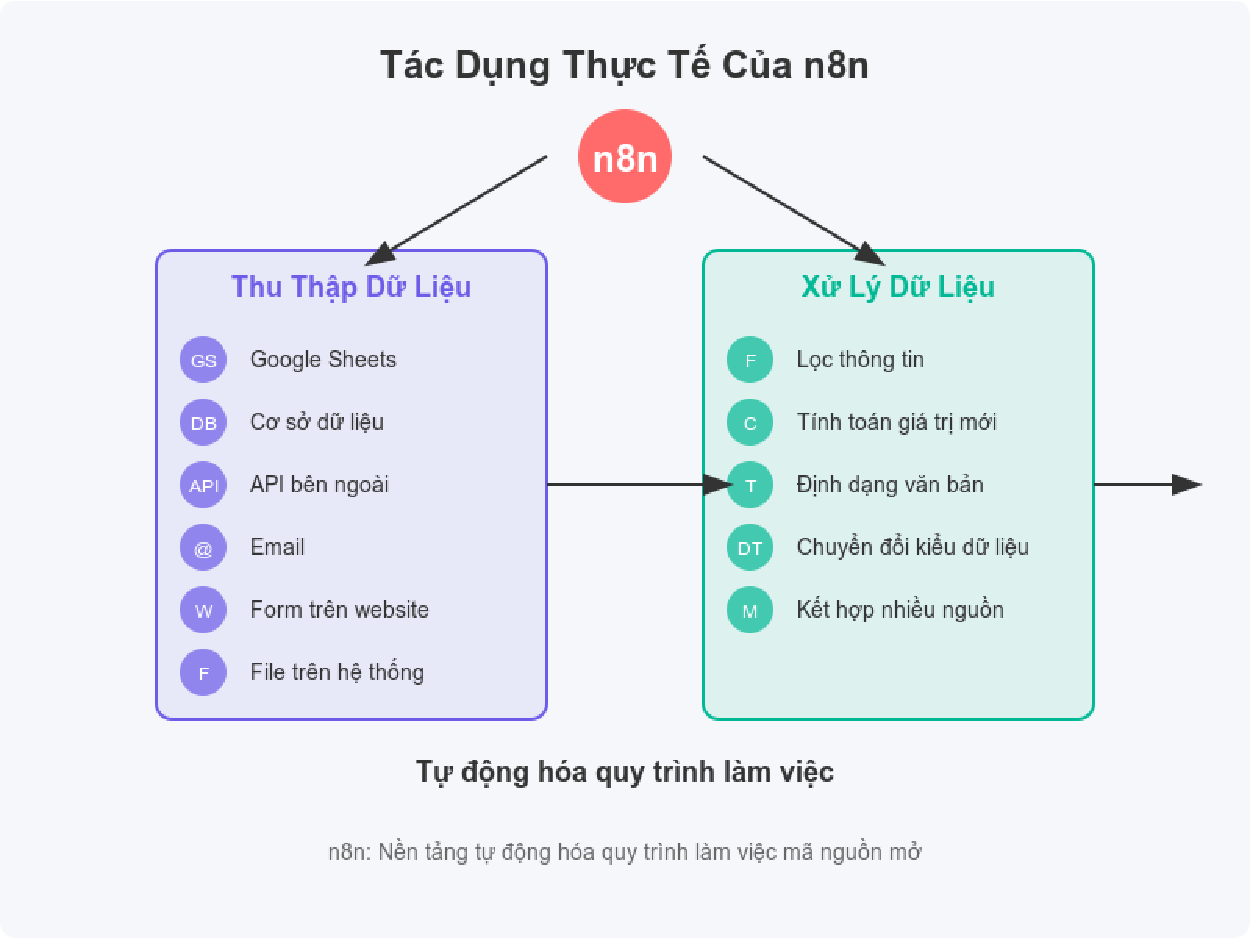
\includegraphics[width=1\linewidth]{Chap1-7/a.pdf}
    \caption{Tác dụng và chức năng thực tế của n8n}
\end{figure}

Các loại node cơ bản:
\begin{itemize}
    \item Trigger: Bắt đầu workflow (ví dụ: Webhook khi có dữ liệu).
    \item Action in app: Gọi tới một node khác không phải n8n (ví dụ: Gửi email).
\end{itemize}
Ví dụ: Nút Webhook giống như chuông cửa – khi có khách (dữ liệu), nó báo cho các nút khác hành động.

\newpage
\section{Cấu trúc của một node}


\subsection{Input}

\begin{figure}[htbp]
    \centering
    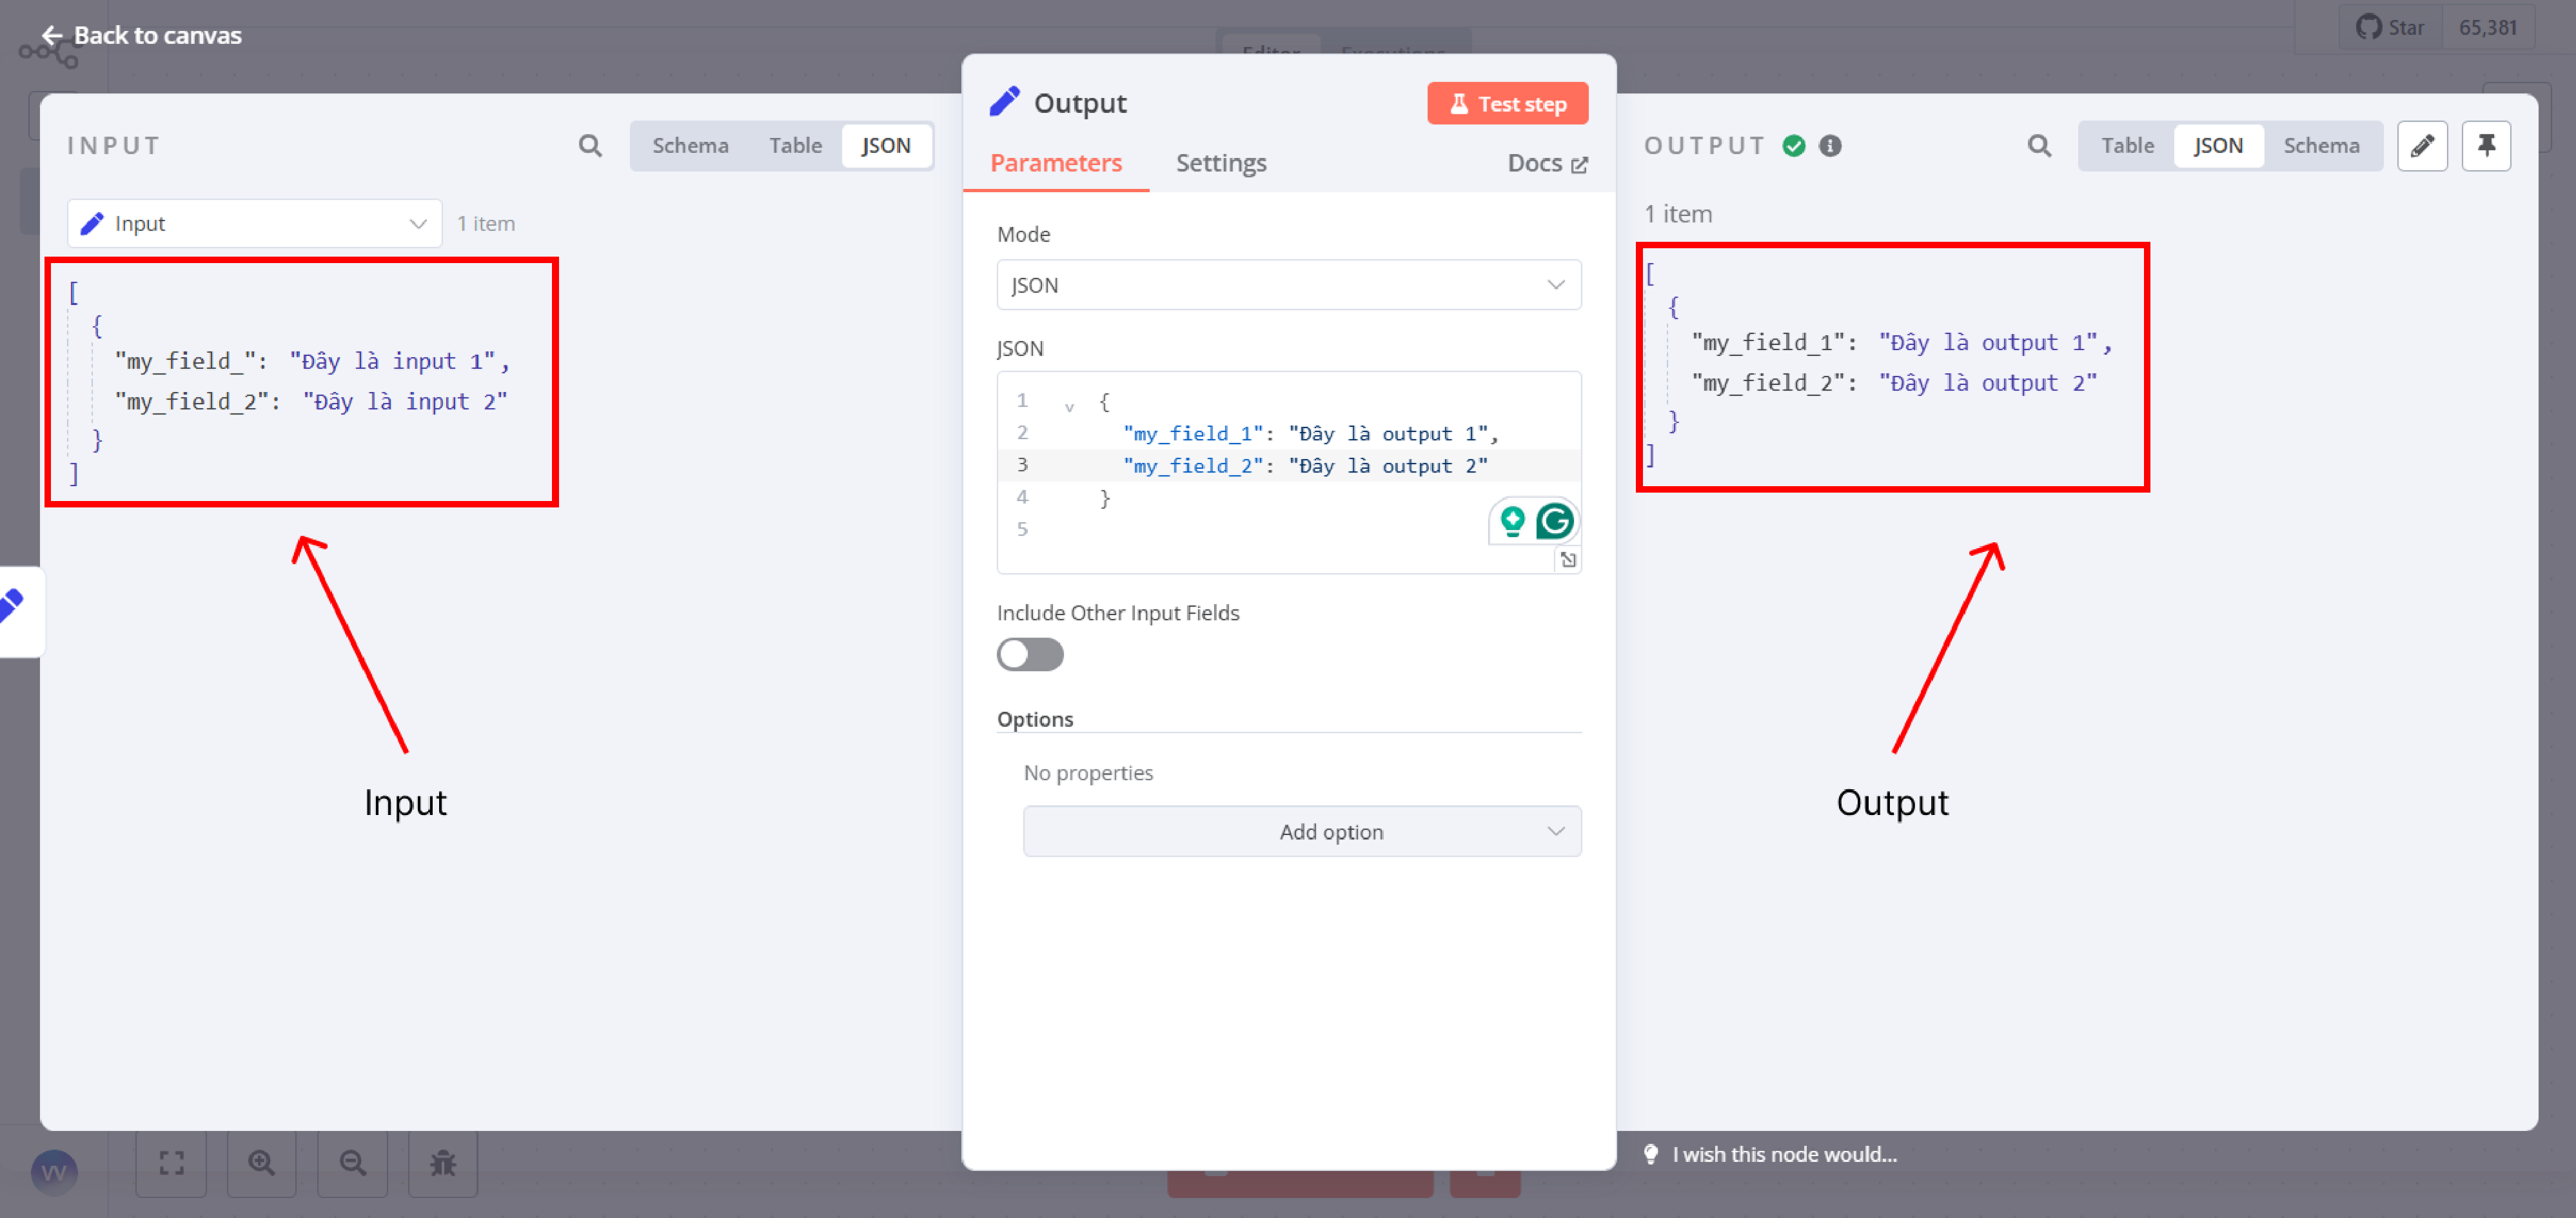
\includegraphics[width=1\linewidth]{Chap1-7/input-ouput.pdf}
\end{figure}

Input là dữ liệu mà node nhận được từ các node trước đó trong workflow. Mỗi node (trừ Trigger nodes) sẽ nhận dữ liệu đầu vào từ một hoặc nhiều node khác.

\begin{lstlisting}[language = Javascript]
{
  "items": [
    {
      "json": {
        "ten": "Nguyen Van A",
        "email": "nguyenvana@example.com",
        "tuoi": 30
      },
      "binary": {
        // Du lieu nhi phan nhu file, hinh anh
      }
    },
    {
      "json": {
        "ten": "Tran Thi B",
        "email": "tranthib@example.com",
        "tuoi": 25
      },
      "binary": {}
    }
  ]
}
\end{lstlisting}
Cấu trúc này có những đặc điểm quan trọng:
\begin{itemize}
    \item Items: Là một mảng các phần tử dữ liệu, mỗi phần tử là một bản ghi riêng biệt
    \item json: Chứa dữ liệu dạng JSON của mỗi item
    \item binary: Chứa dữ liệu nhị phân như file, hình ảnh
\end{itemize}

Khi một node xử lý xong và chuyển dữ liệu sang node tiếp theo, dữ liệu vẫn duy trì cấu trúc này.

\clearpage
\subsection{Parameters}
Parameters là các cài đặt và tùy chọn mà bạn có thể thiết lập cho mỗi node. Chúng quyết định cách node hoạt động và xử lý dữ liệu.

Các loại parameters phổ biến:

\begin{figure}[htbp]
    \centering
    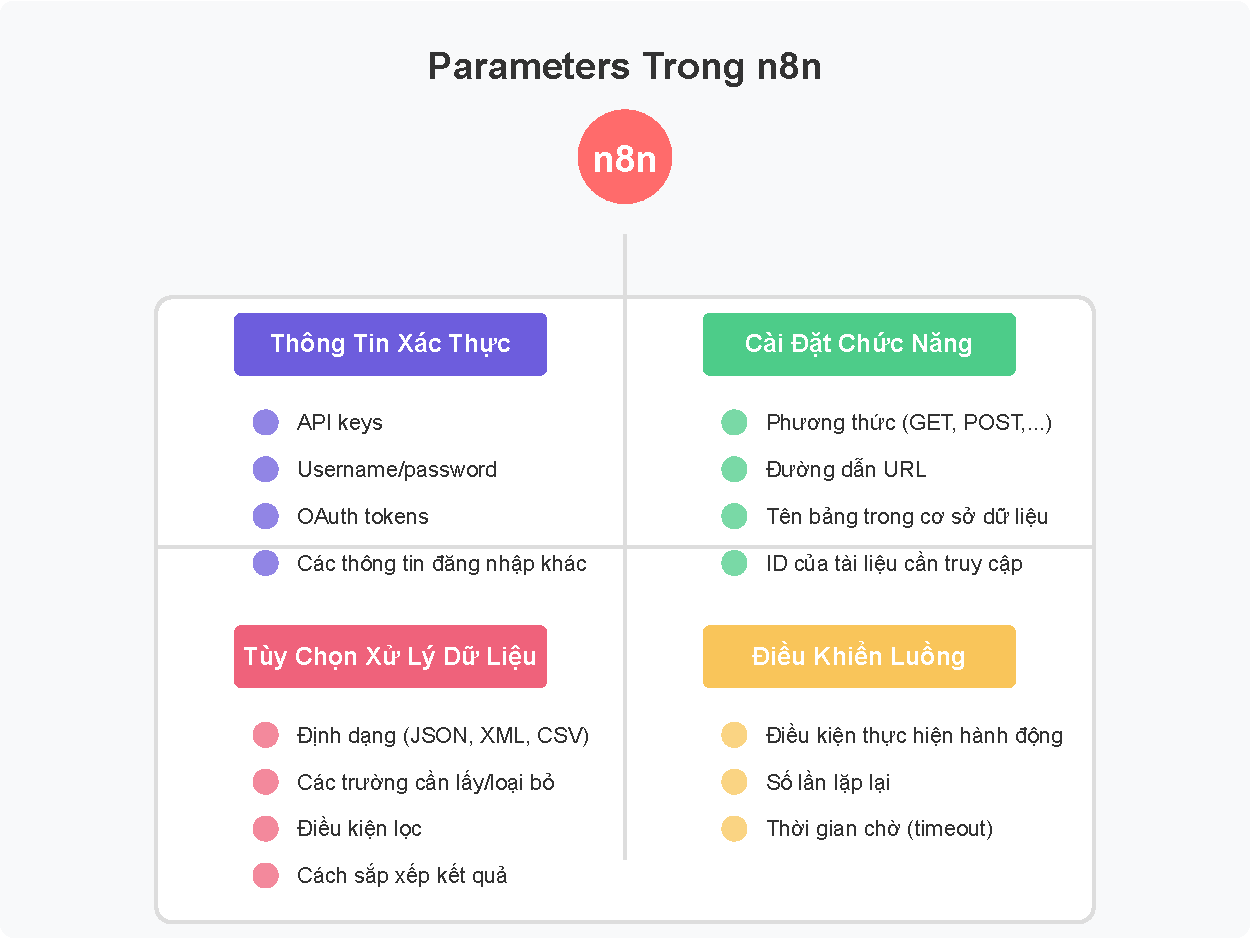
\includegraphics[width=1\linewidth]{Chap1-7/parameters.pdf}
    % \caption{Caption}
\end{figure}

Ví dụ về parameters trong HTTP Request node:
\begin{lstlisting}   
Method: POST
URL: https://api.example.com/users
Headers:
  Content-Type: application/json
  Authorization: Bearer abc123xyz
Query Parameters:
  limit: 10
  offset: 0
Request Body:
  {
    "name": "Nguyen Van A",
    "email": "nguyenvana@example.com"
  }
\end{lstlisting}


\subsection{Output}
Output là kết quả sau khi node thực hiện xong công việc của nó. Output này sẽ trở thành input cho node tiếp theo trong workflow.
Output tuân theo cùng cấu trúc với input:
\begin{itemize}
    \item Mảng các items
    \item Mỗi item có phần json và binary
\end{itemize}

Ví dụ output từ HTTP Request node lấy danh sách người dùng:

\begin{lstlisting}[language = Javascript]   
{
  "items": [
    {
      "json": {
        "id": 1,
        "name": "Nguyen Van A",
        "email": "nguyenvana@example.com",
        "createdAt": "2023-01-15T08:30:00Z"
      }
    },
    {
      "json": {
        "id": 2,
        "name": "Tran Thi B",
        "email": "tranthib@example.com",
        "createdAt": "2023-02-20T10:45:00Z"
      }
    }
  ]
}
\end{lstlisting}


\subsection{Kết nối các nút để tạo luồng dữ liệu}

\begin{figure}[htbp]
    \centering
    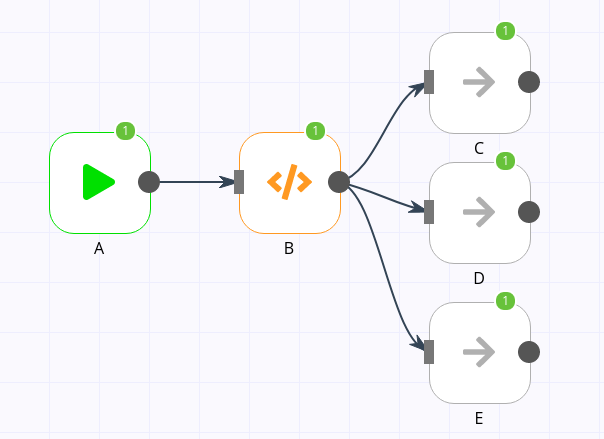
\includegraphics[width=0.6\linewidth]{Chap1-7/node.png}
    \caption{Minh họa node trong n8n}
\end{figure}


\begin{itemize}
    \item Kéo dây từ chấm tròn "Output" của nút này sang chấm tròn "Input" của nút khác.
    \item Dữ liệu sẽ chảy qua dây nối đó.
\end{itemize}

Ví dụ: Nối Webhook với Gmail để dữ liệu từ Webhook được gửi qua email.

\section{Trigger Node}
Trigger nodes là điểm khởi đầu của mọi workflow. Chúng xác định khi nào workflow sẽ được kích hoạt và thực thi. Một workflow luôn bắt đầu bằng ít nhất một trigger node.

\begin{enumerate}
    \item Webhook Node

Webhook node kích hoạt workflow khi nhận được một HTTP request từ bên ngoài.

Ví dụ cấu hình:
\begin{lstlisting}
Method: POST
Path: /new-order
Authentication: username/password
\end{lstlisting}

\textbf{Ứng dụng thực tế:}
\begin{itemize}
    \item Nhận thông báo khi có đơn hàng mới từ website
    \item Tích hợp với dịch vụ thanh toán như PayPal, Stripe
    \item Nhận dữ liệu từ IoT devices
\end{itemize}
\newpage 
\item Cron Node

Cron node kích hoạt workflow theo lịch trình định kỳ, sử dụng cú pháp cron.

Ví dụ cấu hình:
% Làm thế nào đấy để đóng khung cái này vào
\begin{itemize}
    \item 0 9 * * 1-5    (Chạy lúc 9 giờ sáng mỗi ngày từ thứ 2 đến thứ 6)
    \item 0 */2 * * *    (Chạy mỗi 2 giờ)
    \item 0 0 1 * *      (Chạy vào 0 giờ ngày 1 hàng tháng)
\end{itemize}

\textbf{Ứng dụng thực tế:}
\begin{itemize}
    \item Tạo báo cáo hàng ngày/tuần/tháng
    \item Sao lưu dữ liệu định kỳ
    \item Gửi email nhắc nhở
\end{itemize}

\item Email Trigger Node

Email Trigger node kích hoạt workflow khi nhận được email mới phù hợp với tiêu chí đã đặt.

Ví dụ cấu hình:
\begin{itemize}
    \item Email account: support@example.com
    \item Folder: INBOX
    \item Include: Subject contains "urgent"
\end{itemize}

\textbf{Ứng dụng thực tế:}
\begin{itemize}
    \item Tự động phản hồi email
    \item Tạo ticket hỗ trợ từ email
    \item Lưu trữ tệp đính kèm
\end{itemize}

\item Form Trigger Node

Form Trigger node tạo một form online và kích hoạt workflow khi form được submit.

% Ví dụ cấu hình:

% Fields:

% - Name (text)

% - Email (email)

% - Message (textarea)

% - Priority (dropdown: Low, Medium, High)

% Ứng dụng thực tế:

% \begin{itemize}
%     \item Thu thập phản hồi khách hàng
%     \item Đăng ký sự kiện
%     \item Tạo lead từ website
% \end{itemize}

\end{enumerate}

\newpage
\section{Data transformation}

\subsection{Node Set}
\begin{figure}[htbp]
    \centering
    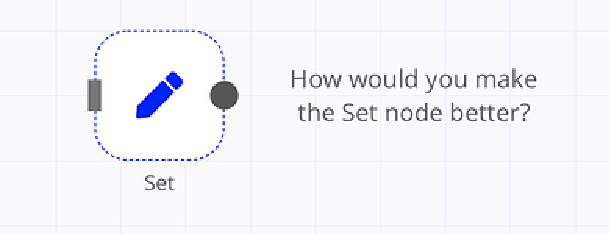
\includegraphics[width=0.8\linewidth]{Chap1-7/set-node.pdf}
\end{figure}

Node này là node rất hay sử dụng. Thường thì mọi người hay cho mình template và sử dụng node set này để thiết lập một số thông tin trong quá trình workflow chạy chúng ta có thể sử dụng node set này để tạo ra các biến mới giúp thông tin gọn gàng hơn

Đây là một node khá đơn giản


1 số cấu hình: "Inputed Fields to include" -> Chọn Selected -> Chỉ chọn biến còn lại bỏ, lấy từ node set trước -> Giúp gọn gàng hơn


\subsection{Split out}

\begin{figure}[htbp]
    \centering
    
\includegraphics[width=0.4\linewidth]{Chap1-7/split-out.pdf}
\end{figure}

Giả sử bạn có đoạn json như này, bạn không có kiến thức về code hay lập trình. Và bạn vẫn muốn cắt đoạn json này thành các bản ghi tương ứng theo dòng và theo đối tượng. Thì node Split out là lựa chọn phù hợp cho bạn.

\begin{verbatim}
{
  "payments": [
    {
      "transactionId": "TXN1001",
      "payerName": "Nguyễn Hoàng Long",
      "amount": 1500000,
      "method": "Chuyển khoản",
      "date": "2025-04-05",
      "status": "Thành công"
    },
    {
      "transactionId": "TXN1002",
      "payerName": "Trần Thu Hà",
      "amount": 850000,
      "method": "Thẻ tín dụng",
      "date": "2025-04-04",
      "status": "Đang xử lý"
    },
    {
      "transactionId": "TXN1003",
      "payerName": "Lê Văn Hùng",
      "amount": 420000,
      "method": "Tiền mặt",
      "date": "2025-04-03",
      "status": "Thất bại"
    }
  ]
}
\end{verbatim}

Split out sẽ lấy các thuộc tính bên trong ra 

\newpage

Kết quả nhận được:

\begin{figure}[htbp]
    \centering
    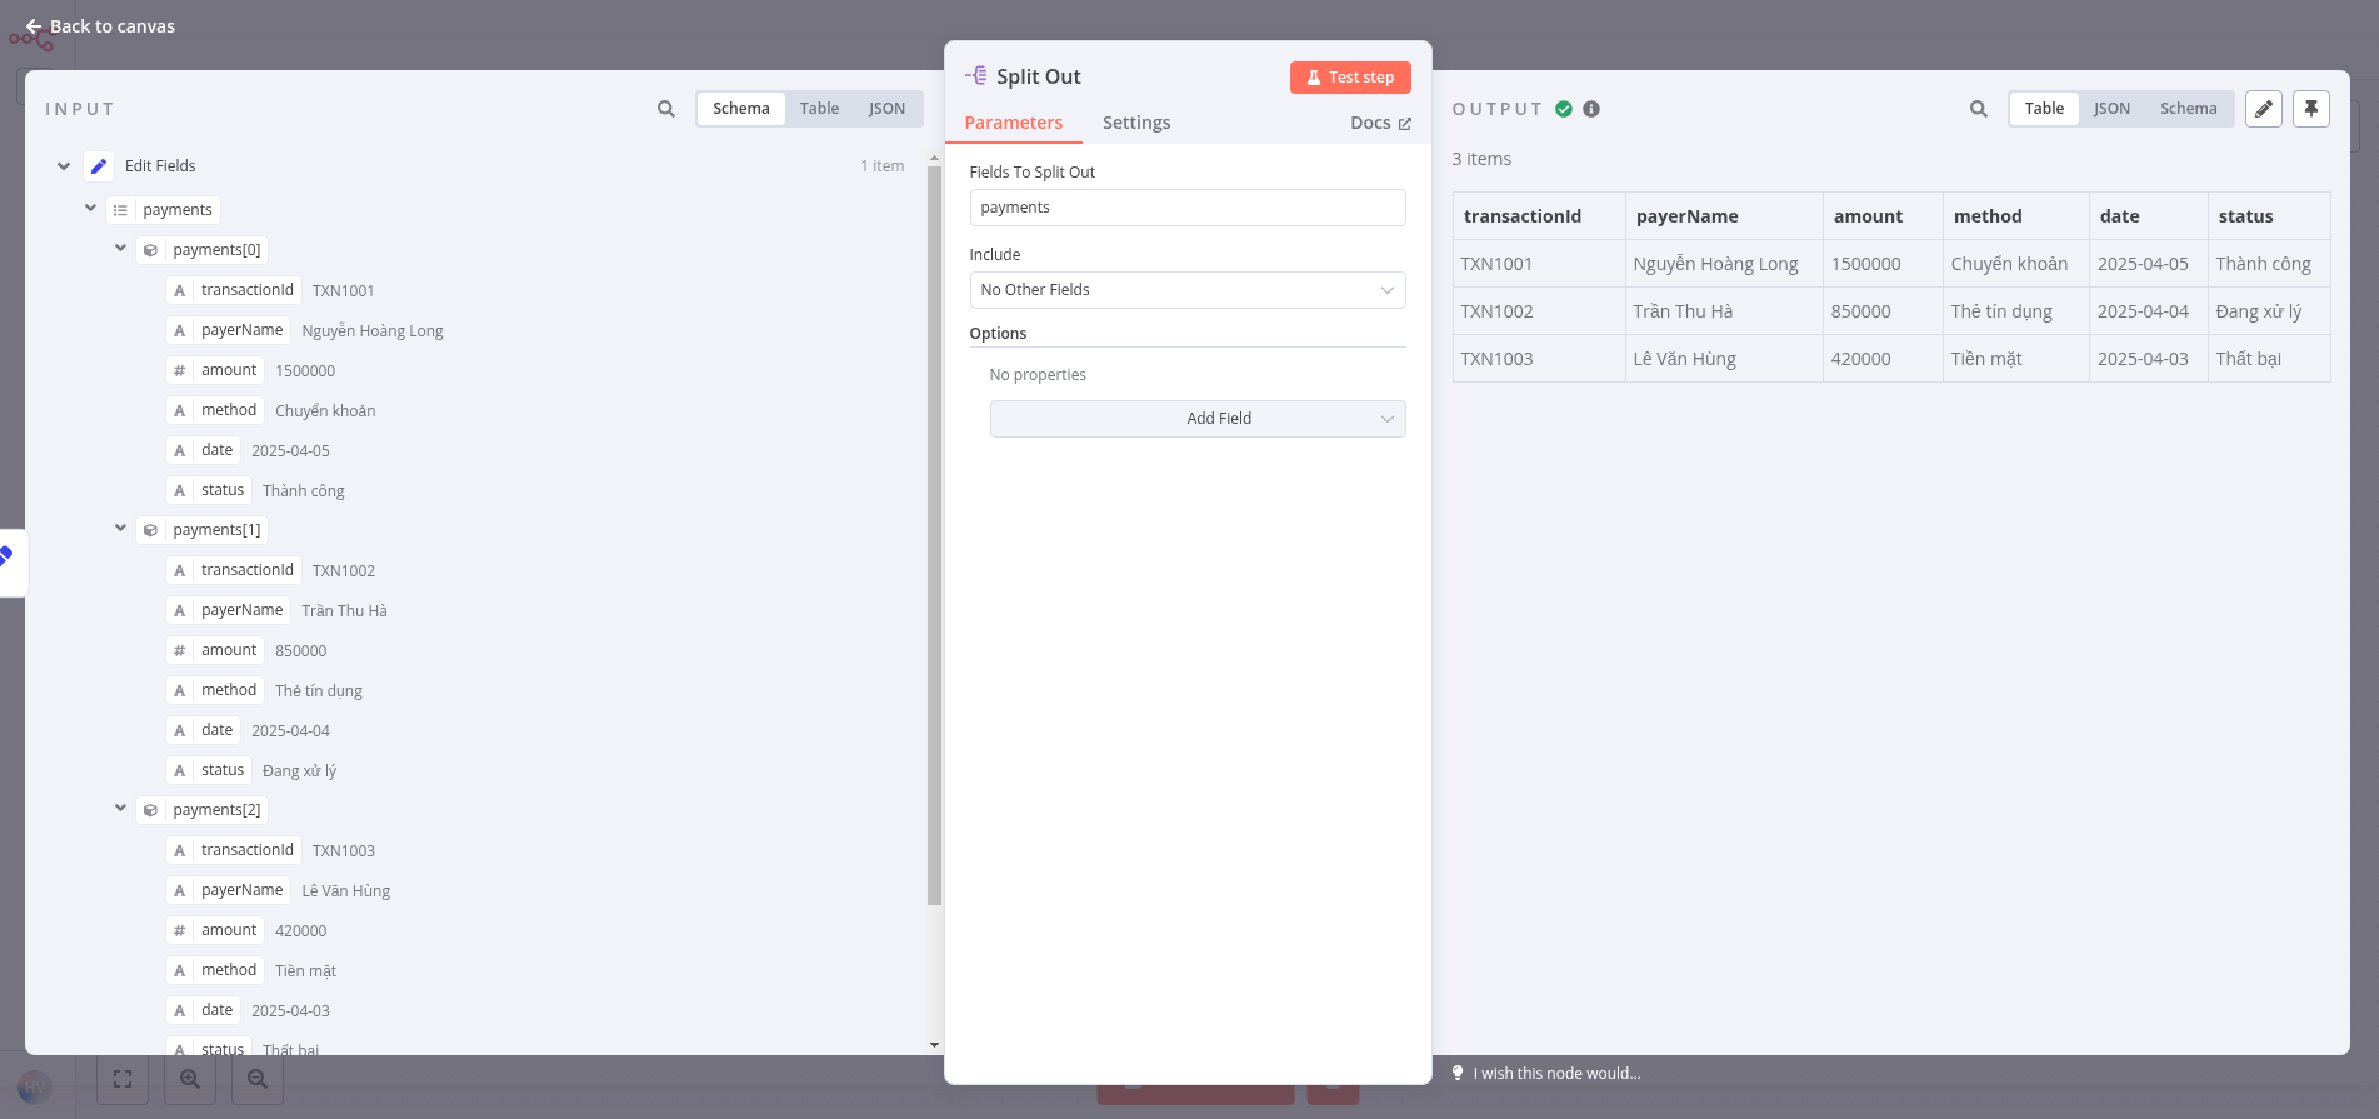
\includegraphics[width=1\linewidth]{Chap1-7/splitout.pdf}
\end{figure}

$\Rightarrow$ Đại khái hiểu cái này như unest trong sql.

\subsection{Node merge}
\begin{figure}[htbp]
    \centering
    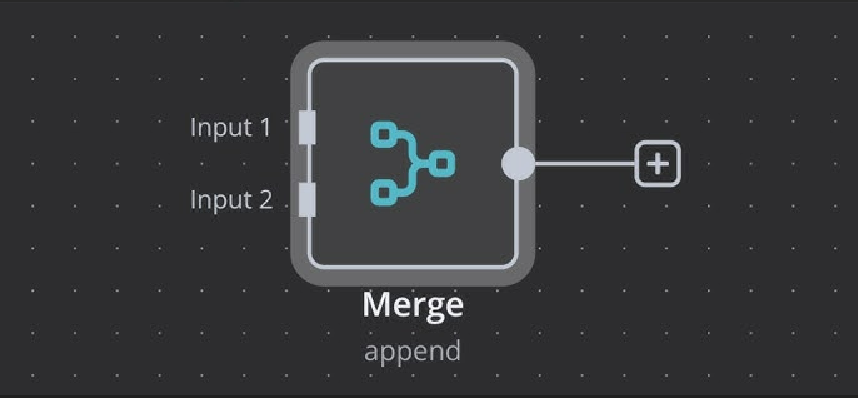
\includegraphics[width=0.8\textwidth]{Chap1-7/merge-merge.pdf}
\end{figure}

Node Merge trong n8n cho phép bạn kết hợp dữ liệu đầu ra từ nhiều node khác nhau thành một luồng dữ liệu duy nhất. Điều này đặc biệt hữu ích khi bạn cần tổng hợp thông tin từ các nguồn khác nhau hoặc khi bạn có các nhánh xử lý song song cần được hợp nhất.

Có nhiều chế độ:

\begin{itemize}
    \item Append
    \item Merge by Fields
    \item Merge by Position
    \item Pass-throught
\end{itemize}
\begin{enumerate}
    \item Append: Thêm vào

Mô tả: Thêm tất cả các mục từ tất cả các đầu vào thành một mảng duy nhất. Sử dụng khi muốn tập hợp tất cả các dữ liệu từ nhiều nguồn mà không cần quan tâm đến việc ghép nối chúng với nhau

    \item Merge By Fields: Hợp nhất theo trường

Mô tả: Kết hợp các mục dựa trên các trường khóa được chỉ định
Trường hợp sử dụng: Khi các mục từ các nguồn khác nhau liên quan đến nhau thông qua một trường chung

    \item Merge By Position: Hợp nhất theo vị trí

Mô tả: Kết hợp các mục dựa trên vị trí của chúng trong mảng
Trường hợp sử dụng: Khi thứ tự của dữ liệu đầu vào tương ứng với nhau

    \item Pass-through: Truyền qua

Mô tả: Truyền qua tất cả các mục từ một đầu vào cụ thể
Trường hợp sử dụng: Khi bạn cần ưu tiên một luồng dữ liệu nhưng vẫn muốn đợi cho đến khi tất cả các kết nối đầu vào đã xử lý xong
\end{enumerate}

$\Rightarrow$ \textit{Phần này là intro thôi, phần sau sẽ kĩ hơn.}


Ngoài ra còn cái node khác cũng rất hữu ích:

- edit filed

- Remove duplicate

- filter

- limit

- Edit image

- Markdown

- Convert

- Extract from file

- HTML


- Crypto

\section{Flow node}

Flow control nodes cho phép bạn kiểm soát cách dữ liệu di chuyển qua workflow, tạo các nhánh rẽ và kết hợp dữ liệu.
\begin{enumerate}
    \item \textbf{IF Node}  
    IF node tạo hai nhánh dựa trên một điều kiện: true (đúng) và false (sai).  

    Ví dụ cấu hình:
\begin{lstlisting}[language=JavaScript]
Condition: {{ $input.item.json.amount > 1000000 }}    
\end{lstlisting}

    Với cấu hình này:
    \begin{itemize}
        \item Nếu giá trị \texttt{amount} lớn hơn 1,000,000, dữ liệu sẽ đi theo nhánh \textbf{TRUE}.
        \item Nếu giá trị \texttt{amount} nhỏ hơn hoặc bằng 1,000,000, dữ liệu sẽ đi theo nhánh \textbf{FALSE}.
    \end{itemize}
    
    \item \textbf{Switch Node}  
    Switch node tạo nhiều nhánh dựa trên giá trị của một trường.  

    Ví dụ cấu hình:
\begin{lstlisting}[language=JavaScript]
Field: {{ $input.item.json.status }}
Case 1: "new" -> Output 1
Case 2: "processing" -> Output 2
Case 3: "completed" -> Output 3
Case 4: "cancelled" -> Output 4
Default: Output 5 (other value)
\end{lstlisting}

    Ứng dụng:
    \begin{itemize}
        \item Định tuyến ticket hỗ trợ dựa trên phòng ban.
        \item Xử lý đơn hàng dựa trên trạng thái.
        \item Phân loại email dựa trên chủ đề.
    \end{itemize}

    \item \textbf{Merge Node}  
    Merge node kết hợp dữ liệu từ nhiều nhánh khác nhau trong workflow.  

    Ví dụ cấu hình:
\begin{verbatim}
Mode: Merge By Position
    - Ghep du lieu theo vi tri (item 1 tu input 1 + item 1 tu input 2)
    
    or
    
Mode: Merge By Fields
    - Truong de ghep: "id"
    - Ghep cac items co cung gia tri id tu cac input khac nhau
\end{verbatim}

    Ứng dụng:
    \begin{itemize}
        \item Kết hợp thông tin khách hàng từ nhiều nguồn.
        \item Ghép dữ liệu đơn hàng với thông tin vận chuyển.
        \item Tạo báo cáo tổng hợp từ nhiều bộ dữ liệu.
    \end{itemize}

    \item \textbf{Split In Batches Node}  
    Split In Batches node chia một tập dữ liệu lớn thành các nhóm nhỏ hơn để xử lý.  

    Ví dụ cấu hình:
\begin{verbatim}
Batch Size: 10
    - Chia du lieu thanh cac nhom, moi nhom 10 items
    - Moi nhom se duoc xu ly tuan tu
\end{verbatim}


    Ứng dụng:
    \begin{itemize}
        \item Xử lý hàng loạt email marketing.
        \item Gửi dữ liệu lớn đến API có giới hạn số lượng request.
        \item Tối ưu hóa hiệu suất khi xử lý dữ liệu lớn.
    \end{itemize}
\end{enumerate}

\subsection{Wait}
Dừng workflow tạm thời tại một điểm nhất định – cho đến khi:
\begin{enumerate}
    \item Một khoảng thời gian trôi qua (Time Duration), hoặc
    \item Đến một thời điểm cụ thể (Specific Date \& Time), hoặc

    \item Khi có tín hiệu từ node Webhook hoặc Wait → Resume (External Resume).
\end{enumerate}

Node này cực kỳ hữu ích khi bạn:
\begin{enumerate}
    \item Gửi email rồi đợi vài giờ mới kiểm tra phản hồi.

    \item Đợi một sự kiện từ người dùng (qua webhook).

    \item Chờ đến một thời điểm cụ thể (ví dụ: đến 9h sáng hôm sau mới gửi báo cáo
\end{enumerate}

\subsection{Kết nối giữa các Nodes}

Các nodes trong n8n được kết nối với nhau để tạo ra luồng dữ liệu. Dữ liệu sẽ di chuyển từ trigger node đến input nodes, sau đó qua các bước xử lý và cuối cùng đến output nodes. Việc kết nối này giúp đảm bảo rằng dữ liệu được truyền tải một cách mạch lạc và tự động hóa quy trình làm việc hiệu quả hơn.

$\Rightarrow$ \textit{Tóm lại, cấu trúc của một workflow trong n8n bao gồm Trigger Node để khởi động quy trình, Input Nodes để thu thập dữ liệu đầu vào, và Output Nodes để thực hiện các hành động dựa trên dữ liệu đó.}


\subsection{Mẹo sử dụng Node hiệu quả}

\begin{itemize}
    \item Đặt tên rõ ràng: Gọi node là "Gửi Email Nhắc Nhở" thay vì để mặc định "Email1" để dễ theo dõi.
    \item Kiểm tra từng bước: Dùng nút "Execute Node" để kiểm tra từng node trước khi chạy toàn bộ workflow.
    \item Tận dụng dữ liệu giữa các Node: Dữ liệu từ node trước (như thời gian từ Cron) có thể được dùng ở node sau (như thêm thời gian vào email).
\end{itemize}


\section{Core node}

\subsection{HTTP request}
Trước khi đi sâu vào Node HTTP Request hãy chậm lại để hiểu về API đã. Web API hoạt động dựa trên cùng nền tảng công nghệ quen thuộc với hầu hết các trang web bạn lướt qua hàng ngày trên internet. Nhưng thay vì mang đến những trang web yêu thích hay những đoạn video mèo con đáng yêu, các máy chủ web được thiết lập để vận hành API mở ra cánh cửa cho các hệ thống từ xa gửi yêu cầu và nhận về dữ liệu phản hồi dựa trên thông tin đầu vào. Dữ liệu luân chuyển giữa các hệ thống này thường được gói gọn trong định dạng JSON – gọn gàng và đầy sức mạnh!

Để chứng kiến một API cơ bản hoạt động, hãy thử nghiệm với Random User API. Mở trình duyệt của bạn và nhập vào thanh địa chỉ: https://randomuser.me/api/. Thoạt nhìn, bạn có thể thấy một chuỗi ký tự khó hiểu, nhưng nếu quan sát kỹ, bạn sẽ nhận ra một vài điểm tương đồng với những gì chúng ta đã học ở chương về node Function. Thứ bạn đang thấy chính là JSON ở dạng nén hoặc chưa được định dạng đẹp mắt!

Để truy cập được API, một thứ item thiết yếu phải cần là URL. Việc hiểu rõ và thiết kế API vô cùng quan trọng vì bạn luôn muốn điều chỉnh đầu ra để đạt được kết quả mong muốn. 


Thử quan sát một API và phân tích nó:

\begin{verbatim}
https://api.example.com/v3/computers?type=laptop&ram=32&hdd=1024
\end{verbatim}

Các thành phần của một URL API

\begin{enumerate}
    \item Giao thức (Protocol)

Trong ví dụ trên, phần https:// chính là giao thức.

Thông thường, giao thức sẽ là http:// hoặc https://.

Điều quan trọng cần nhớ là nếu dùng http://, dữ liệu sẽ không được mã hóa giữa máy khách và máy chủ API, có thể dẫn đến rủi ro bảo mật.

Vì vậy, luôn đảm bảo sử dụng https:// để đảm bảo an toàn cho dữ liệu.

    \item Base URL

Trong ví dụ, api.example.com chính là base URL, đôi khi còn được gọi là hostname, domain name hoặc DNS name.
Đây là địa chỉ máy chủ nơi API được lưu trữ.

    \item Endpoint
    
Endpoint trong URL trên là /v3/computers, đôi khi được gọi là API path.
Endpoint có thể là tĩnh (không thay đổi) hoặc động (thay đổi dựa trên dữ liệu được yêu cầu).

Ví dụ trên có hai phần:

/v3 → Cho biết đây là phiên bản thứ 3 của API.

/computers → Chỉ ra rằng API này sẽ trả về thông tin về một hoặc nhiều máy tính.

    \item  Query Parameters
    

\tcbset{colback=red!5!white,colframe=red!75!black}
\begin{tcolorbox}[title=Các tham số truy vấn trong ví dụ là:]
\begin{itemize}
    \item type=laptop

    \item ram=32

    \item hdd=1024
\end{itemize}
\end{tcolorbox}


\tcbset{colback=red!5!white,colframe=red!75!black}
\begin{tcolorbox}[title=Chúng được xác định bởi hai dấu phân cách:]
\begin{itemize}
    \item Dấu ? → Tách các tham số truy vấn khỏi phần còn lại của URL.

    \item Dấu \& → Ngăn cách từng tham số truy vấn.

    \item Tương tự như trong JSON, mỗi tham số có dạng cặp key-value:
    \begin{itemize}
        \item key → Phần trước dấu =.

       \item value → Phần sau dấu =.
    \end{itemize}

\end{itemize}
\end{tcolorbox}


Các thành phần khác trong API Request
\begin{enumerate}
    \item Headers



\tcbset{colback=orange!5!white,colframe=orange!75!black}
\begin{tcolorbox}[title=Headers chứa metadata về request API chẳng hạn như:]
\begin{itemize}
    \item Loại dữ liệu truyền tải.

    \item Token xác thực.

    \item Thông tin về máy chủ.

    \item Headers thường có định dạng key-value.
\end{itemize}
\end{tcolorbox}



    \item Body Parameters
Body chứa dữ liệu được gửi kèm trong request, thường có dạng key-value.

Các phương thức HTTP (HTTP Methods)
Các phương thức HTTP là cách để API xử lý request từ client.


\tcbset{colback=green!5!white,colframe=green!75!black}
\begin{tcolorbox}[title=Dưới đây là một số phương thức phổ biến:]
\begin{itemize}
    \item GET → Lấy dữ liệu từ API (tương tự khi truy cập một trang web).

    \item POST → Gửi dữ liệu mới đến API để lưu trữ.

    \item DELETE → Xóa một tài nguyên hoặc bản ghi trên máy chủ API.

    \item HEAD → Giống GET nhưng chỉ trả về phần header, không có dữ liệu.

    \item PATCH → Cập nhật một phần thông tin trong bản ghi hiện có.

    \item PUT → Nếu bản ghi đã tồn tại, ghi đè dữ liệu cũ bằng dữ liệu mới; nếu chưa có, tạo bản ghi mới.
\end{itemize}
\end{tcolorbox}




Khi gửi request đến API, máy chủ sẽ trả về một mã phản hồi để báo trạng thái của request:

\tcbset{colback=green!5!white,colframe=green!75!black}
\begin{tcolorbox}[title=Mã phản hồi HTTP (Response Codes)]
\begin{itemize}
    \item 1xx (Thông tin) → Máy chủ đã nhận request và đang xử lý.

    \item 2xx (Thành công) → Request đã được xử lý thành công.

    \item 3xx (Chuyển hướng) → API đã được di chuyển đến một địa chỉ khác.

    \item 4xx (Lỗi từ phía client) → Request bị sai, cần kiểm tra và chỉnh sửa.

    \item 5xx (Lỗi từ phía server) → Máy chủ API có vấn đề, không thể xử lý request.
\end{itemize}
\end{tcolorbox}

Bây giờ, khi đã hiểu rõ về API URL, chúng ta sẽ bắt đầu sử dụng HTTP Request node trong n8n để kết nối với API! 
\end{enumerate}

\end{enumerate}



\subsection{Code}

Bạn nghĩ rằng n8n là công cụ nocode và bạn sẽ có node phù hợp cho workflow của bạn. Thật không may không có node nào là đa năng cả. Điều này hoàn toàn dễ hiểu do trong thực tế có vô vàn điều có thể xảy ra. 

$\Rightarrow$ \textit{Vì vậy n8n tạo ra Function Code cho phép thực thi mã Javascript để xử lý các trường hợp khó bằng code. }

Không giống như nhiều node khác có sẵn các tùy chọn và tham số để lựa chọn, Function node chỉ có duy nhất một tham số—trường nhập mã JavaScript. Toàn bộ thao tác xử lý dữ liệu của bạn sẽ được thực hiện trong trường này.

Trong JavaScript code field, bạn sẽ viết mã JavaScript để thao tác dữ liệu bên trong Function node.
Mặc dù bạn không cần phải là một chuyên gia về JavaScript, nhưng việc hiểu cơ bản về ngôn ngữ này sẽ mang lại nhiều lợi ích. Đối với nội dung trong cuốn sách này, chỉ cần nắm vững những kiến thức JavaScript cơ bản là đủ.


\subsection{Webhook}
Node Webhook hoạt động như một "người nghe" - khi có sự kiện xảy ra, webhook sẽ nhận thông báo và kích hoạt hành động tương ứng.

\textbf{Tính năng chính:}

\begin{itemize}
    \item Hỗ trợ các phương thức HTTP: GET, POST, PUT, DELETE
    \item Xác thực với Basic Auth hoặc Header Auth  
    \item Tự động phân tích dữ liệu JSON, form data và query parameters
    \item Có thể tạo phản hồi tùy chỉnh cho người gửi request
\end{itemize}

Ví dụ: Bot thông báo thời tiết đơn giản:

\begin{enumerate}
    \item Tạo một node Webhook với phương thức POST ở path \texttt{/weather}
    \item Khi có request gửi đến với dữ liệu: \texttt{\{"city": "Hanoi"\}}
    \item Sử dụng HTTP Request node để gọi API thời tiết với thành phố từ request
    \item Định dạng kết quả và gửi thông báo thời tiết qua Telegram
    \item Trả về phản hồi thành công cho request ban đầu
\end{enumerate}

\textbf{Gọi webhook}
\begin{lstlisting}
curl -X POST https://n8n.yourdomain.com/webhook/weather \
  -H "Content-Type: application/json" \
  -d '{"city": "Hanoi"}'
\end{lstlisting}

Người dùng sẽ nhận được thông báo: \textit{"Thời tiết tại Hanoi hiện tại là 28°C, trời quang. Độ ẩm: 75\%"} thông qua Telegram, và webhook sẽ trả về phản hồi: \texttt{\{"status": "success", "message": "Weather info sent"\}}.

\textbf{Lưu ý quan trọng}
Webhook chỉ hoạt động khi workflow được kích hoạt. URL Webhook là duy nhất cho mỗi node và cần cẩn thận về bảo mật khi sử dụng công khai. Node Webhook là điểm khởi đầu lý tưởng cho các workflow tự động được kích hoạt bởi dữ liệu từ các dịch vụ bên ngoài.

\section{Human in loop}
Trong một quy trình tự động hóa, không phải lúc nào cũng có thể (hoặc nên) để máy móc quyết định tất cả. Có những bước yêu cầu sự xem xét, phê duyệt hoặc đánh giá từ con người – đây là lúc các node Human in the Loop phát huy vai trò.

Bộ node Human in the Loop trong n8n cho phép bạn "tạm dừng" workflow tại một điểm nhất định, chờ phản hồi từ người dùng, rồi tiếp tục xử lý dựa trên phản hồi đó. Bộ node này bao gồm:

\textbf{Ví dụ ứng dụng:}
\begin{enumerate}
    \item Quy trình duyệt chi phí: Khi nhân viên nộp yêu cầu thanh toán, workflow sẽ gửi yêu cầu đến quản lý để phê duyệt. Sau khi người quản lý bấm "Duyệt" hoặc "Từ chối", quy trình tiếp tục dựa theo lựa chọn.

    \item Phê duyệt gửi email hàng loạt: Trước khi gửi email marketing đến hàng ngàn khách hàng, workflow tạo một HITL request để người phụ trách xác nhận nội dung và danh sách gửi.

    \item Xác nhận dữ liệu nghi vấn: Trong các bước xử lý dữ liệu, nếu phát hiện giá trị bất thường, workflow có thể hỏi người dùng để xác nhận thông tin trước khi tiếp tục.
\end{enumerate}

\section{Regular Nodes}
Regular nodes là những node thực hiện các hành động cụ thể trong workflow. Chúng xử lý dữ liệu đầu vào và tạo ra dữ liệu đầu ra mới.
\begin{enumerate}
    \item  HTTP Request Node: gửi các request đến API hoặc website bên ngoài.

Ví dụ cấu hình cho việc tạo người dùng mới:
\begin{lstlisting}[language = Javascript] 
Method: POST
URL: https://api.example.com/users
Headers:
  Content-Type: application/json
  Authorization: Bearer YOUR_TOKEN
Body (JSON):
  {
    "name": "{{ $input.item.json.name }}",
    "email": "{{ $input.item.json.email }}",
    "role": "user"
  }
\end{lstlisting}

\item Google Sheets Node: cho phép tương tác với bảng tính Google Sheets.


Ví dụ cấu hình để thêm dữ liệu:
\begin{lstlisting}[language = Javascript]    
Operation: Append Row
Spreadsheet ID: 1abc...xyz
Sheet Name: Orders
Fields:
  Order ID: {{ $input.item.json.id }}
  Customer: {{ $input.item.json.customerName }}
  Amount: {{ $input.item.json.total }}
  Date: {{ $now.format("YYYY-MM-DD") }}
\end{lstlisting}

\item Function Node: cho phép thực thi mã JavaScript hoặc Python tùy chỉnh để xử lý dữ liệu.

Ví dụ hàm tính tổng và trung bình:
\begin{lstlisting}[language = Javascript]
// Khoi tao bien tong
let tong = 0;

// Lap qua moi item va tinh tong
for (const item of items) {
  tong += item.json.amount;
}

// Tinh trung binh
const trungBinh = tong / items.length;

// Tra ve ket qua nhu mot item moi
return [{
  json: {
    tongAmount: tong,
    trungBinhAmount: trungBinh,
    soLuongGiaoDich: items.length,
    ngay: new Date().toISOString()
  }
}];

// Vi du ham lam sach du lieu:
const itemsDaLamSach = [];

// Xu ly tung item
for (const item of items) {
  // Sao chep item de khong thay doi item goc
  const itemLamSach = {
    json: { ...item.json }
  };
  
  // Lam sach du lieu
  if (itemLamSach.json.email) {
    itemLamSach.json.email = itemLamSach.json.email.toLowerCase().trim();
  }
  
  if (itemLamSach.json.phone) {
    // Loai bo cac ky tu khong phai so
    itemLamSach.json.phone = itemLamSach.json.phone.replace(/\D/g, '');
  }
  
  if (itemLamSach.json.name) {
    // Chuan hoa chu cai dau tien viet hoa
    itemLamSach.json.name = itemLamSach.json.name
      .trim()
      .split(' ')
      .map(word => word.charAt(0).toUpperCase() + word.slice(1).toLowerCase())
      .join(' ');
  }
  
  itemsDaLamSach.push(itemLamSach);
}

return itemsDaLamSach;
\end{lstlisting}

Với node này bạn chỉ cần tư duy để xử lý các logic đơn giản với code. 

\item Email Send Node: node gửi email với nội dung tùy chỉnh.

Ví dụ cấu hình:
\begin{verbatim}
To: {{ $input.item.json.customerEmail }}
Subject: Don hang #{{ $input.item.json.orderId }} da duoc xac nhan
Body (HTML):
  <p>Xin chao {{ $input.item.json.customerName }},</p>
  <p>Cam on ban da dat hang. Don hang #{{ $input.item.json.orderId }} cua ban da duoc xac nhan.</p>
  <p>Tong gia tri: {{ $input.item.json.total.toLocaleString() }} VND</p>
  <p>Thoi gian giao hang du kien: 3-5 ngay lam viec</p>
\end{verbatim}

\item Telegram Node: bot gửi tin nhắn qua Telegram.

Ví dụ cấu hình:

\begin{verbatim}
Operation: Send Message
Chat ID: {{ $input.item.json.telegramId }}
Text: news: {{ $input.item.json.notificationTitle }}
\end{verbatim}

\end{enumerate}




\section{Expressions}
Expressions là một tính năng mạnh mẽ trong n8n cho phép bạn tạo các giá trị động, xử lý dữ liệu, và tùy chỉnh cách node hoạt động.
\subsection{Sử dụng Expressions}
Để sử dụng expressions trong n8n:

\textbf{Bước 1: Kích hoạt chế độ expression}
\begin{itemize}
    \item Nhấp vào biểu tượng "=" bên cạnh trường bạn muốn sử dụng expression
    \item Trường sẽ chuyển sang chế độ expression, được đánh dấu bằng cặp dấu {{ }}
    \item Hoặc nhập trực tiếp \{\{ và nội dung expression của bạn
\end{itemize}

\textbf{Bước 2: Viết expression}
\begin{itemize}
    \item Sử dụng cú pháp JavaScript
    \item Truy cập dữ liệu đầu vào qua biến \$ input
    \item Sử dụng các biến và hàm có sẵn của n8n
\end{itemize}

\textbf{Bước 3: Kiểm tra expression}

Nhấp vào nút "Test" bên cạnh trường
Xem kết quả của expression

Ví dụ truy cập dữ liệu đơn giản:
\begin{lstlisting}[language = Javascript]    
{{ $input.item.json.customerName }}
\end{lstlisting}

Truy cập trường customerName

Ví dụ thực hiện phép tính tổng giá trị
\begin{lstlisting}[language = Javascript]    
{{ $input.item.json.price * $input.item.json.quantity }} 
\end{lstlisting}

Ví dụ nối chuỗi họ và tên
\begin{lstlisting}[language = Javascript]    
{{ $input.item.json.firstName + ' ' + $input.item.json.lastName }}
\end{lstlisting}
\subsection{Các Biểu Thức Phổ Biến}
\begin{enumerate}
    \item Truy cập dữ liệu đầu vào
\begin{lstlisting}[language = Javascript]   
{{ $input.item.json.fieldName }}
\end{lstlisting}

 Truy cập một phần tử trong mảng
\begin{lstlisting}[language = Javascript]
{{ $input.item.json.items[0].name }}
\end{lstlisting}
Kiểm tra nếu trường tồn tại
\begin{lstlisting}[language = Javascript]
{{ $input.item.json.hasOwnProperty('email') ? $input.item.json.email : 'unknown' }}
\end{lstlisting}
\item Xử lý chuỗi

Chuyển đổi chuỗi thành chữ hoa/chữ thường
\begin{lstlisting}[language = Javascript]
{{ $input.item.json.name.toUpperCase() }}
{{ $input.item.json.email.toLowerCase() }}
\end{lstlisting}

Cắt chuỗi
\begin{lstlisting}[language = Javascript]
{{ $input.item.json.description.substring(0, 100) + '...' }}
\end{lstlisting}

Loại bỏ khoảng trắng
\begin{lstlisting}[language = Javascript]
{{ $input.item.json.code.trim() }}
\end{lstlisting}

Thay thế nội dung
\begin{lstlisting}[language = Javascript]
{{ $input.item.json.address.replace('Street', 'St.') }}
\end{lstlisting}
\item Xử lý số

Làm tròn số
\begin{lstlisting}[language = Javascript]
{{ Math.round($input.item.json.amount) }}
\end{lstlisting}

 Định dạng số với 2 chữ số thập phân
\begin{lstlisting}[language = Javascript]
{{ $input.item.json.price.toFixed(2) }}
\end{lstlisting}

Tính giá sau thuế (10\%)
\begin{lstlisting}[language = Javascript]
{{ $input.item.json.price * 1.1 }}
\end{lstlisting}

Tìm giá trị lớn nhất
\begin{lstlisting}[language = Javascript]
{{ Math.max($input.item.json.price1, $input.item.json.price2, $input.item.json.price3) }}
\end{lstlisting}
\item Xử lý ngày tháng
\begin{lstlisting}[language = Javascript]
{{ new Date().toISOString() }}

\end{lstlisting}

Định dạng ngày
\begin{lstlisting}[language = Javascript]
{{ new Date($input.item.json.createdAt).toLocaleDateString('vi-VN') }}
\end{lstlisting}

Tính số ngày giữa hai ngày
\begin{lstlisting}[language = Javascript]
{{ Math.floor((new Date() - new Date($input.item.json.orderDate)) / (1000 * 60 * 60 * 24)) }}
\end{lstlisting}

Thêm 30 ngày vào một ngày
\begin{lstlisting}[language = Javascript]
{{ new Date(new Date($input.item.json.startDate).getTime() + 30 * 24 * 60 * 60 * 1000).toISOString() }}
\end{lstlisting}
\item Xử lý logic

Toán tử điều kiện
\begin{lstlisting}[language = Javascript]
{{ $input.item.json.age >= 18 ? 'Adult' : 'Minor' }}
\end{lstlisting}

Kiểm tra nhiều điều kiện
\begin{lstlisting}[language = Javascript]
{{ $input.item.json.score > 90 ? 'A' : $input.item.json.score > 80 ? 'B' :
\end{lstlisting}
\end{enumerate}


% Chương 4
\chapter{Làm việc với dữ liệu trong n8n}

\section{Biến, JSON, Expressions}

\subsection{Biến trong n8n: Cách lưu trữ và sử dụng thông tin}

Trong cuộc sống hàng ngày, chúng ta thường ghi chú thông tin để sử dụng sau này. Trong n8n, ``biến'' chính là những ghi chú kỹ thuật số.

\subsubsection{Ví dụ: Tự động gửi tin nhắn chào mừng}

Giả sử bạn muốn chào mừng khách hàng mới đăng ký:

\begin{enumerate}
    \item Tạo biến workflow để lưu lời chào:
    \begin{verbatim}
    welcomeMessage: Chào mừng bạn đến với dịch vụ của chúng tôi!
    companyName: Công ty ABC
    \end{verbatim}

    \item Khi có người đăng ký, sử dụng biến trong email:
    \begin{verbatim}
    Tiêu đề: {{ $vars.welcomeMessage }}
    Nội dung: Cảm ơn bạn đã đăng ký dịch vụ của {{ $vars.companyName }}
    \end{verbatim}
\end{enumerate}

% \begin{figure}[h]
%     \centering
%     \includegraphics[width=0.8\textwidth]{images/bien-trong-workflow-email}
%     \caption{Biến trong workflow thực tế}
%     \label{fig:bien-workflow}
% \end{figure}

\textbf{Cách thiết lập biến đơn giản:}
\begin{enumerate}
    \item Mở workflow
    \item Nhấp vào biểu tượng bánh răng
    \item Chọn ``Variables''
    \item Thêm tên và giá trị cho biến
\end{enumerate}

\subsection{JSON: Ngôn ngữ dữ liệu của n8n}

JSON giống như một bảng thông tin có tổ chức. Ví dụ, thông tin người dùng trong JSON:

\begin{verbatim}
{
  "hoTen": "Nguyễn Văn A",
  "email": "nguyenvana@example.com",
  "soDienThoai": "0912345678",
  "diaChi": {
    "duong": "Lê Lợi",
    "quan": "Hoàn Kiếm",
    "thanhPho": "Hà Nội"
  }
}
\end{verbatim}

\subsubsection{Thu thập thông tin biểu mẫu từ website}

Khi khách hàng điền form trên website:
\begin{enumerate}
    \item Thông tin được gửi đến n8n dưới dạng JSON
    \item Mỗi mục thông tin là một cặp key-value
    \item Dữ liệu có thể lồng nhau (như địa chỉ ở trên)
\end{enumerate}

\subsection{Expressions: Công cụ làm việc với dữ liệu}

(bổ sung cho phần trên)

Expressions giống như công thức trong Excel, giúp bạn tính toán và xử lý dữ liệu.

\subsubsection{Ví dụ: Tính giá sau giảm giá}

Giả sử bạn có shop online và muốn tính giá sau khi giảm 10\%:

\begin{enumerate}
    \item Trong Set node, tạo trường ``giaSauGiamGia'':
    \begin{verbatim}
    {{ $json.giaBanDau * 0.9 }}
    \end{verbatim}

    \item Định dạng giá tiền:
    \begin{verbatim}
    {{ ($json.giaSauGiamGia).toFixed(0).toString()
    .replace(/\B(?=(\d{3})+(?!\d))/g, ".") }}
    \end{verbatim}
\end{enumerate}

% \begin{figure}[h]
%     \centering
%     \includegraphics[width=0.8\textwidth]{images/expressions-tinh-gia}
%     \caption{Expressions tính giá giảm 10\%}
%     \label{fig:expressions-gia}
% \end{figure}

\textbf{Ứng dụng thực tế khác:}
\begin{enumerate}
    \item Chuyển đổi định dạng ngày: \verb|{{ new Date($json.ngayDatHang).toLocaleDateString('vi-VN') }}|
    \item Ghép họ và tên: \verb|{{ $json.ho + ' ' + $json.ten }}|
    \item Kiểm tra điều kiện: \verb|{{ $json.tuoi >= 18 ? 'Người lớn' : 'Trẻ em' }}|
\end{enumerate}

\section{Storage Node (Data, Cache, Database)}

\subsection{Data Storage: Lưu trữ thông tin giữa các lần chạy}

\subsubsection{Ví dụ: Đếm số lượt truy cập website}

\begin{enumerate}
    \item Mỗi khi có người truy cập:
    \begin{itemize}
        \item Lấy số lượt hiện tại từ Data Storage
        \item Tăng thêm 1
        \item Lưu lại vào Data Storage
    \end{itemize}
\end{enumerate}

% \begin{figure}[h]
%     \centering
%     \includegraphics[width=0.8\textwidth]{images/workflow-dem-luot-truy-cap}
%     \caption{Workflow đếm lượt truy cập website}
%     \label{fig:dem-luot-truy-cap}
% \end{figure}

\textbf{Các bước thực hiện:}
\begin{enumerate}
    \item Thêm HTTP Trigger (kích hoạt khi có truy cập)
    \item Thêm Data Storage node đầu tiên:
    \begin{itemize}
        \item Operation: Get
        \item Key name: visitCount
    \end{itemize}
    \item Thêm Function node để tăng số:
    \begin{verbatim}
    // Nếu chưa có dữ liệu, bắt đầu từ 0
    const currentCount = items[0].json.data ?
    parseInt(items[0].json.data) : 0;
    
    // Tăng thêm 1
    return [{ json: { count: currentCount + 1 } }];
    \end{verbatim}
    \item Thêm Data Storage node thứ hai:
    \begin{itemize}
        \item Operation: Set
        \item Key name: visitCount
        \item Value: \verb|{{ $json.count }}|
    \end{itemize}
\end{enumerate}

\subsection{Cache Node: Lưu trữ tạm thời}

\subsubsection{Ví dụ: Lưu cache kết quả tỷ giá tiền tệ}

Thay vì gọi API tỷ giá mỗi phút, bạn có thể:
\begin{enumerate}
    \item Gọi API tỷ giá
    \item Lưu kết quả vào Cache với thời hạn 1 giờ
    \item Các request trong 1 giờ tiếp theo sẽ dùng dữ liệu cache
\end{enumerate}

% \begin{figure}[h]
%     \centering
%     \includegraphics[width=0.8\textwidth]{images/workflow-cache-ty-gia}
%     \caption{Workflow cache tỷ giá tiền tệ}
%     \label{fig:cache-ty-gia}
% \end{figure}

\textbf{Thiết lập workflow:}
\begin{enumerate}
    \item Thêm Schedule Trigger (chạy mỗi phút)
    \item Thêm Cache node:
    \begin{itemize}
        \item Operation: Get
        \item Key name: exchangeRates
    \end{itemize}
    \item Thêm node IF (kiểm tra cache có dữ liệu không)
    \item Nếu không có dữ liệu:
    \begin{itemize}
        \item Gọi API tỷ giá qua HTTP Request
        \item Lưu kết quả vào Cache:
        \begin{itemize}
            \item Operation: Set
            \item Key name: exchangeRates
            \item TTL: 3600 (1 giờ)
        \end{itemize}
    \end{itemize}
\end{enumerate}

\subsection{Database Node: Làm việc với cơ sở dữ liệu}

\subsubsection{Ví dụ: Hệ thống đặt hàng đơn giản}

\begin{enumerate}
    \item \textbf{Lưu đơn hàng mới:}
    \begin{itemize}
        \item Khách điền form $\rightarrow$ HTTP Trigger nhận dữ liệu
        \item Lưu thông tin vào database:
        \begin{itemize}
            \item Operation: Insert
            \item Table: donhang
            \item Columns \& Values: thông tin từ form
        \end{itemize}
    \end{itemize}
\end{enumerate}


\begin{enumerate}\setcounter{enumi}{1}
    \item \textbf{Cập nhật trạng thái đơn hàng:}
    \begin{itemize}
        \item Admin cập nhật $\rightarrow$ HTTP Trigger
        \item Cập nhật database:
        \begin{itemize}
            \item Operation: Update
            \item Table: donhang
            \item Set: \verb|{{ $json }}|
            \item Where: id = \verb|{{ $json.id }}|
        \end{itemize}
    \end{itemize}

    \item \textbf{Tạo báo cáo đơn hàng theo ngày:}
    \begin{itemize}
        \item Trigger chạy vào cuối ngày
        \item Truy vấn database:
        \begin{itemize}
            \item Operation: Select
            \item Table: donhang
            \item Where: ngayDatHang = today
        \end{itemize}
        \item Gửi email báo cáo tới quản lý
    \end{itemize}
\end{enumerate}

\section{HTTP Request \& API Basics}

\subsection{Tương tác với API: Lấy thông tin từ dịch vụ bên ngoài}

\subsubsection{Ví dụ: Bot thời tiết Telegram}

Khi người dùng nhắn tên thành phố, bot sẽ:
\begin{enumerate}
    \item Nhận tin nhắn từ Telegram
    \item Lấy thông tin thời tiết từ API
    \item Gửi thông tin thời tiết về cho người dùng
\end{enumerate}

\begin{figure}[htbp]
    \centering
    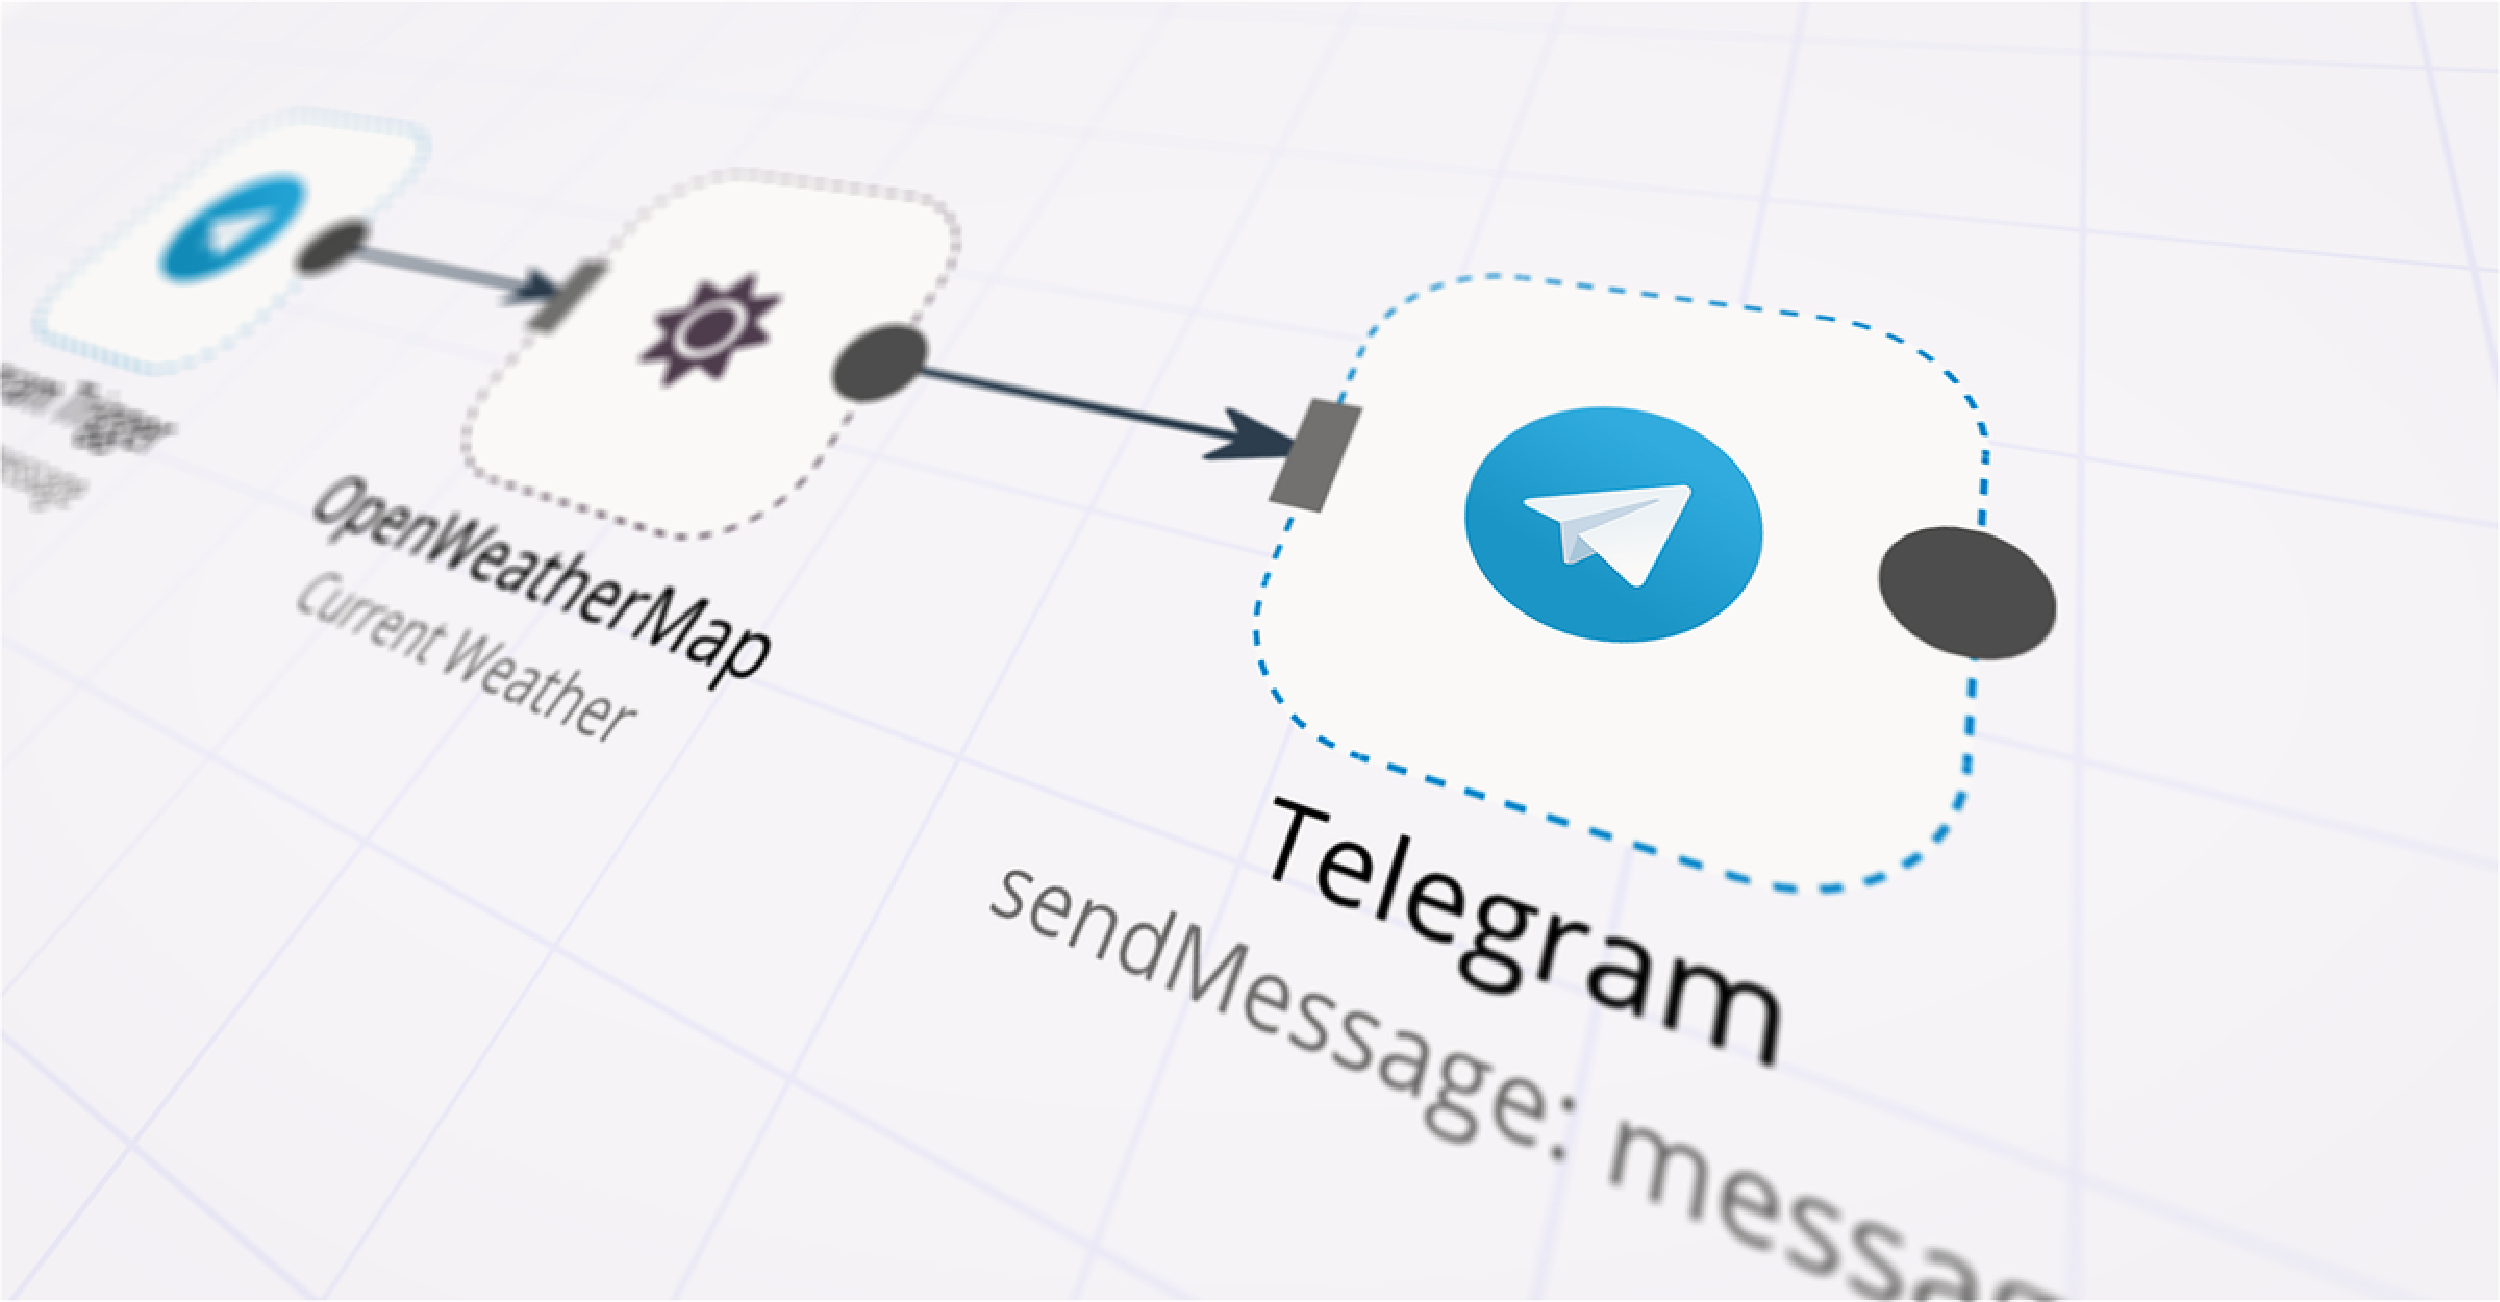
\includegraphics[width=0.8\textwidth]{Chap1-7/tele-weather.pdf}
    \caption{Workflow bot thời tiết Telegram}
\end{figure}

\textbf{Các bước thực hiện:}
\begin{enumerate}
    \item Thêm Telegram Trigger
    \item Thêm HTTP Request node:
    \begin{itemize}
        \item Method: GET
        \item URL: \verb|https://api.openweathermap.org/data/2.5/weather|
        \item Query Parameters:
        \begin{itemize}
            \item q: \verb|{{ $json.content }}| (tên thành phố từ người dùng)
            \item appid: YOUR\_API\_KEY
            \item units: metric
            \item lang: vi
        \end{itemize}
    \end{itemize}
    \item Thêm Function node để định dạng tin nhắn:
    \begin{verbatim}
    const weather = items[0].json;
    return [{
      json: {
        chatId: $node["Telegram Trigger"].json.message.chat.id,
        content: `Thời tiết tại ${weather.name}:\n` +
                 `Nhiệt độ: ${weather.main.temp}°C\n` +
                 `Độ ẩm: ${weather.main.humidity}%\n` +
                 ` Trạng thái: ${weather.weather[0].description}`
      }
    }];
    \end{verbatim}
    \item Thêm Telegram node để gửi tin nhắn lại cho người dùng
\end{enumerate}

\subsection{Xác thực API: Kết nối an toàn với dịch vụ bên ngoài}

\subsubsection{Ví dụ: Tự động đăng bài lên Facebook Page}

Để đăng bài lên Facebook, bạn cần:
\begin{enumerate}
    \item Lấy Access Token từ Facebook
    \item Sử dụng token trong API call
\end{enumerate}

Có hình
% \begin{figure}[h]
%     \centering
%     \includegraphics[width=0.8\textwidth]{images/workflow-dang-facebook}
%     \caption{Workflow đăng bài Facebook}
%     \label{fig:dang-facebook}
% \end{figure}

\textbf{Thiết lập workflow:}
\begin{enumerate}
    \item Thêm HTTP Trigger (khi có bài viết mới)
    \item Thêm HTTP Request node:
    \begin{itemize}
        \item Method: POST
        \item URL: \verb|https://graph.facebook.com/v16.0/YOUR_PAGE_ID/feed|
        \item Query Parameters:
        \begin{itemize}
            \item access\_token: YOUR\_ACCESS\_TOKEN
            \item message: \verb|{{ $json.content }}|
            \item link: \verb|{{ $json.link }}| (nếu có)
        \end{itemize}
    \end{itemize}
\end{enumerate}

\subsection{Tích hợp dịch vụ: Kết nối nhiều hệ thống}

\subsubsection{Ví dụ: Hệ thống CRM đơn giản}

Khi có khách hàng mới từ website:
\begin{enumerate}
    \item Lưu thông tin vào Google Sheets
    \item Tạo task theo dõi trong Trello
    \item Gửi email thông báo cho nhân viên
\end{enumerate}

Có hình
% \begin{figure}[h]
%     \centering
%     \includegraphics[width=0.8\textwidth]{images/workflow-crm-don-gian}
%     \caption{Workflow CRM đơn giản}
%     \label{fig:crm-don-gian}
% \end{figure}

\textbf{Các bước thực hiện:}
\begin{enumerate}
    \item Thêm Webhook node (nhận thông tin từ form)
    \item Thêm Google Sheets node:
    \begin{itemize}
        \item Operation: Append
        \item Spreadsheet: Danh sách khách hàng
        \item Range: Sheet1!A:E
    \end{itemize}
    \item Thêm Trello node:
    \begin{itemize}
        \item Operation: Create Card
        \item List: Khách hàng mới
        \item Title: \verb|Liên hệ {{ $json.hoTen }}|
        \item Description: \verb|{{ $json.email }} - {{ $json.soDienThoai }}|
    \end{itemize}
    \item Thêm Send Email node để thông báo cho nhân viên
\end{enumerate}

\subsection{Xử lý lỗi API: Đảm bảo workflow hoạt động ổn định}

\subsubsection{Ví dụ: Backup dữ liệu từ hệ thống cũ sang mới}

Khi chuyển dữ liệu, cần xử lý các trường hợp lỗi:

Có hình
% \begin{figure}[h]
%     \centering
%     \includegraphics[width=0.8\textwidth]{images/workflow-xu-ly-loi-api}
%     \caption{Workflow xử lý lỗi API}
% \end{figure}

\textbf{Thiết lập workflow:}
\begin{enumerate}
    \item Thêm Trigger (bắt đầu chuyển dữ liệu)
    \item Thêm HTTP Request node để lấy dữ liệu từ hệ thống cũ
    \item Thêm IF node để kiểm tra kết quả:
    \begin{itemize}
        \item Condition: \verb|{{ $json.statusCode }}| Equals \verb|200|
    \end{itemize}
    \item Nếu thành công:
    \begin{itemize}
        \item Thêm HTTP Request để gửi dữ liệu lên hệ thống mới
    \end{itemize}
    \item Nếu thất bại:
    \begin{itemize}
        \item Thêm Send Email node để thông báo lỗi
        \item Lưu lỗi vào log file
    \end{itemize}
\end{enumerate}

\newpage
\section{Bài tập thực hành}
\begin{enumerate}
    \item Tạo workflow gửi email chào mừng khách hàng mới với biến \verb|welcomeMessage| và \verb|companyName|.
    \item Thiết lập workflow tính giá sau giảm giá 15\% với Expressions và định dạng giá tiền.
    \item Thiết kế workflow lưu số lượt truy cập website bằng Data Storage.
    \item Xây dựng workflow cache kết quả giá vàng từ API trong 30 phút bằng Cache node.
    \item Tạo workflow lưu đơn hàng vào database và gửi email thông báo cho admin.
    \item Tạo bot Telegram trả lời thông tin thời tiết dựa trên tên thành phố người dùng gửi.
    \item Thiết lập workflow tự động đăng bài lên Facebook Page sử dụng API và Access Token.
    \item Xây dựng workflow nhận khách hàng mới từ website, lưu vào Google Sheets và tạo thẻ Trello.
    \item Tạo workflow backup dữ liệu giữa hai hệ thống, xử lý lỗi API và gửi email khi thất bại.
\end{enumerate}


% Chương 5
\chapter{Điều kiện và vòng lặp trong workflow}

\section{Giới thiệu}

Các workflow thực tế thường yêu cầu logic phức tạp hơn việc thực hiện các bước một cách tuần tự. Đôi khi bạn cần thực hiện các tác vụ khác nhau dựa trên điều kiện, hoặc lặp lại một tác vụ nhiều lần. Chương này sẽ giới thiệu cách sử dụng các nút điều kiện và vòng lặp trong n8n để tạo các workflow linh hoạt và mạnh mẽ.

\section{If, Switch, Merge Node}

\subsection{IF Node - Điều kiện cơ bản}

IF Node là nút điều kiện cơ bản trong n8n, cho phép workflow rẽ nhánh dựa trên các điều kiện được định nghĩa.

\subsubsection{Cách hoạt động của IF Node}

IF Node đánh giá một hoặc nhiều điều kiện và định tuyến dữ liệu đến ``True'' hoặc ``False'' dựa trên kết quả đánh giá:

\begin{figure}[htbp]
    \centering
    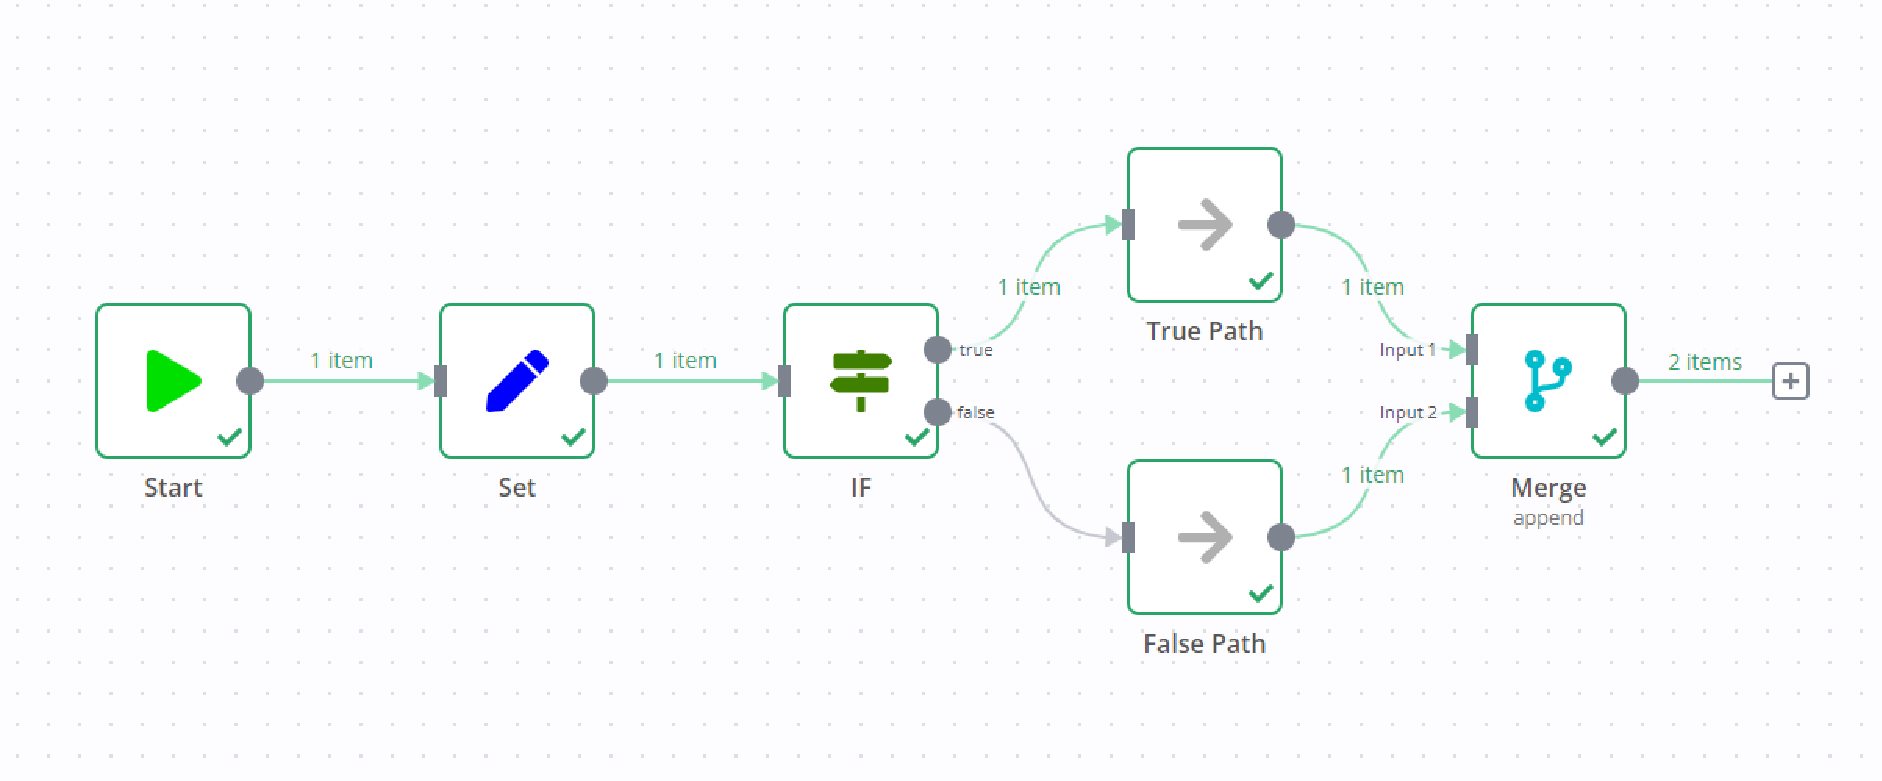
\includegraphics[width=1\linewidth]{Chap1-7/if-merge-node.pdf}
\end{figure} 

\newpage

\subsubsection{Cấu hình IF Node}

\begin{enumerate}
  \item \textbf{Thêm IF Node vào workflow}:
  \begin{itemize}
    \item Tìm và thêm ``IF'' từ thư viện nút.
  \end{itemize}

  \item \textbf{Thiết lập điều kiện}:
  \begin{itemize}
    \item Mỗi điều kiện bao gồm ba thành phần: Giá trị 1, Toán tử so sánh, Giá trị 2.
    \item Ví dụ: \texttt{\{\{\$json["status"]\}\}} \texttt{equals} \texttt{"success"}.
  \end{itemize}
$\Rightarrow$  \textit{Đoạn này với từng điều kiện là text hay số thì phải chọn toán tử so sánh tương ứng.}
  \item \textbf{Kết hợp nhiều điều kiện}:
  \begin{itemize}
    \item Bạn có thể thêm nhiều điều kiện và kết hợp chúng bằng ``AND'' hoặc ``OR''.
    \item AND: Tất cả các điều kiện phải đúng.
    \item OR: Chỉ cần một điều kiện đúng.
  \end{itemize}
\end{enumerate}

\subsubsection{Ví dụ: Xử lý phản hồi API}

Giả sử bạn đang gọi một API để lấy dữ liệu thời tiết và muốn thông báo khi nhiệt độ vượt quá ngưỡng. Truy cập \href{https://www.weatherapi.com/my/}{openweathermap} để lấy api thời tiết miễn phí. 

\begin{figure}[htbp]
    \centering
    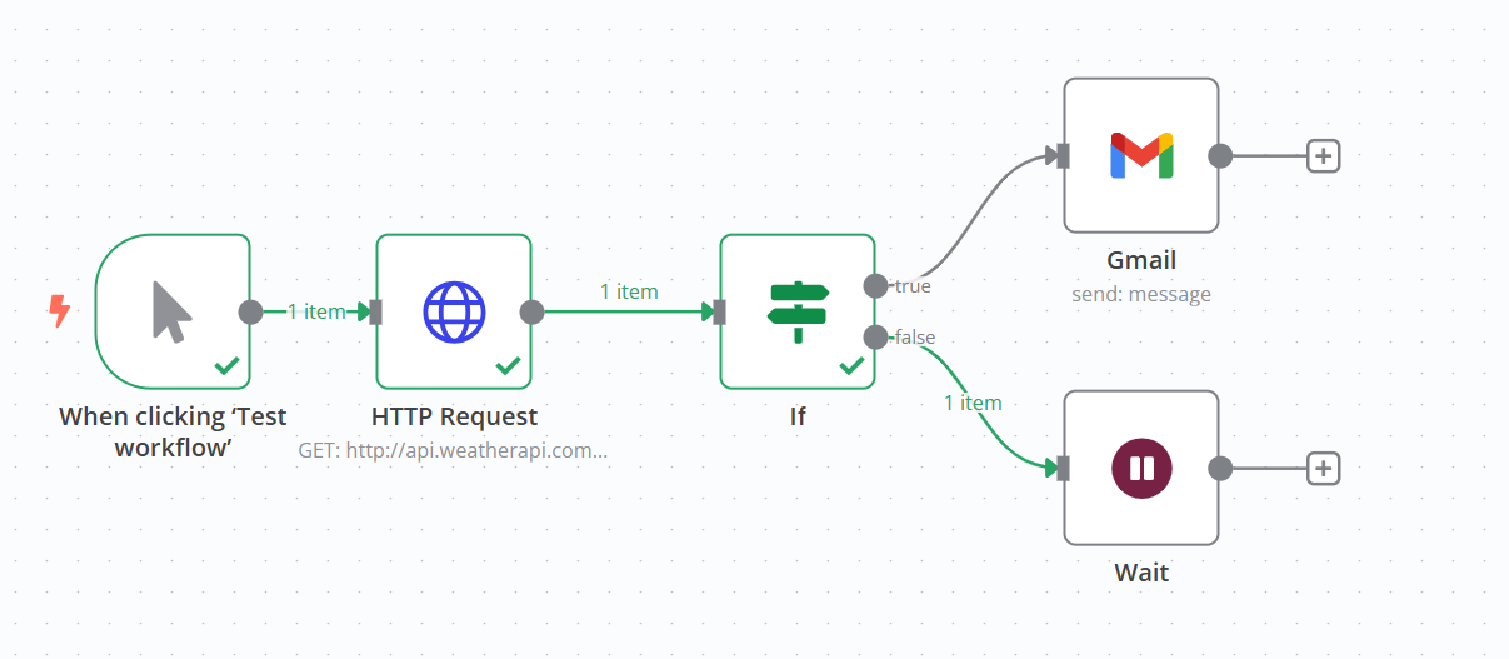
\includegraphics[width=1\linewidth]{Chap1-7/weather.pdf}
    \caption{Workflow thông báo thời tiết}
\end{figure} 

Cấu hình IF Node:

\begin{itemize}
  \item Điều kiện: \texttt{\{\{\$json["temperature"]\}\}} \texttt{larger} \texttt{30}
  \item Nếu thời tiết nóng hơn 30°C, gửi email cảnh báo.
\end{itemize}

\newpage

\subsection{Switch Node - Nhiều nhánh điều kiện}

Switch Node mở rộng khái niệm của IF Node bằng cách cho phép nhiều đường dẫn khác nhau, không chỉ True/False.
\subsubsection{Cách hoạt động của Switch Node}

Switch Node đánh giá một giá trị và định tuyến dữ liệu theo nhiều nhánh khác nhau dựa trên kết quả.

\begin{figure}[htbp]
    \centering
    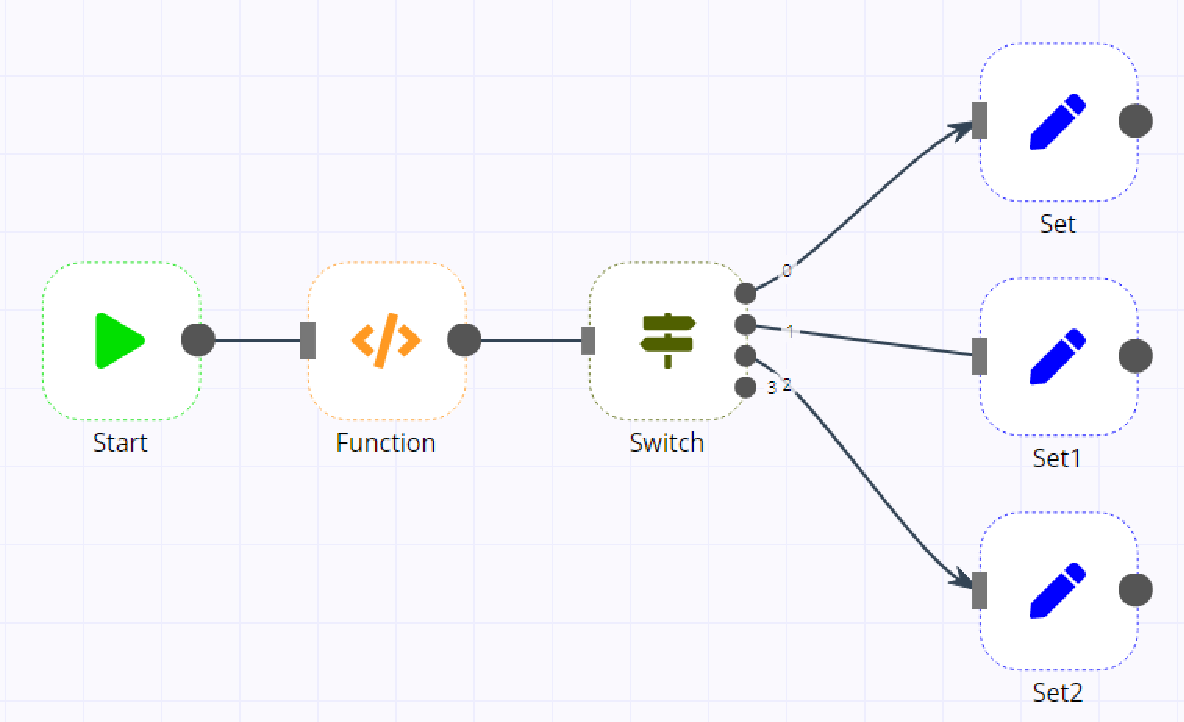
\includegraphics[width=1\linewidth]{Chap1-7/switch_node.pdf}
\end{figure}

\subsubsection{Cấu hình Switch Node}

\begin{enumerate}
  \item \textbf{Thêm Switch Node vào workflow}:
  \begin{itemize}
    \item Tìm và thêm ``Switch'' từ thư viện nút.
  \end{itemize}

  \item \textbf{Thiết lập giá trị đánh giá}:
  \begin{itemize}
    \item Chọn trường dữ liệu để đánh giá (Value to Switch On).
    \item Ví dụ: \texttt{\{\{\$json["status"]\}\}}
  \end{itemize}

  \item \textbf{Định nghĩa các nhánh đầu ra}:
  \begin{itemize}
    \item Thêm trường Output cho mỗi giá trị có thể.
    \item Đặt tên cho mỗi nhánh.
    \item Xác định giá trị khớp.
  \end{itemize}
\end{enumerate}

\newpage
\subsubsection{Ví dụ: Phân loại khách hàng}

\begin{figure}[htbp]
    \centering
    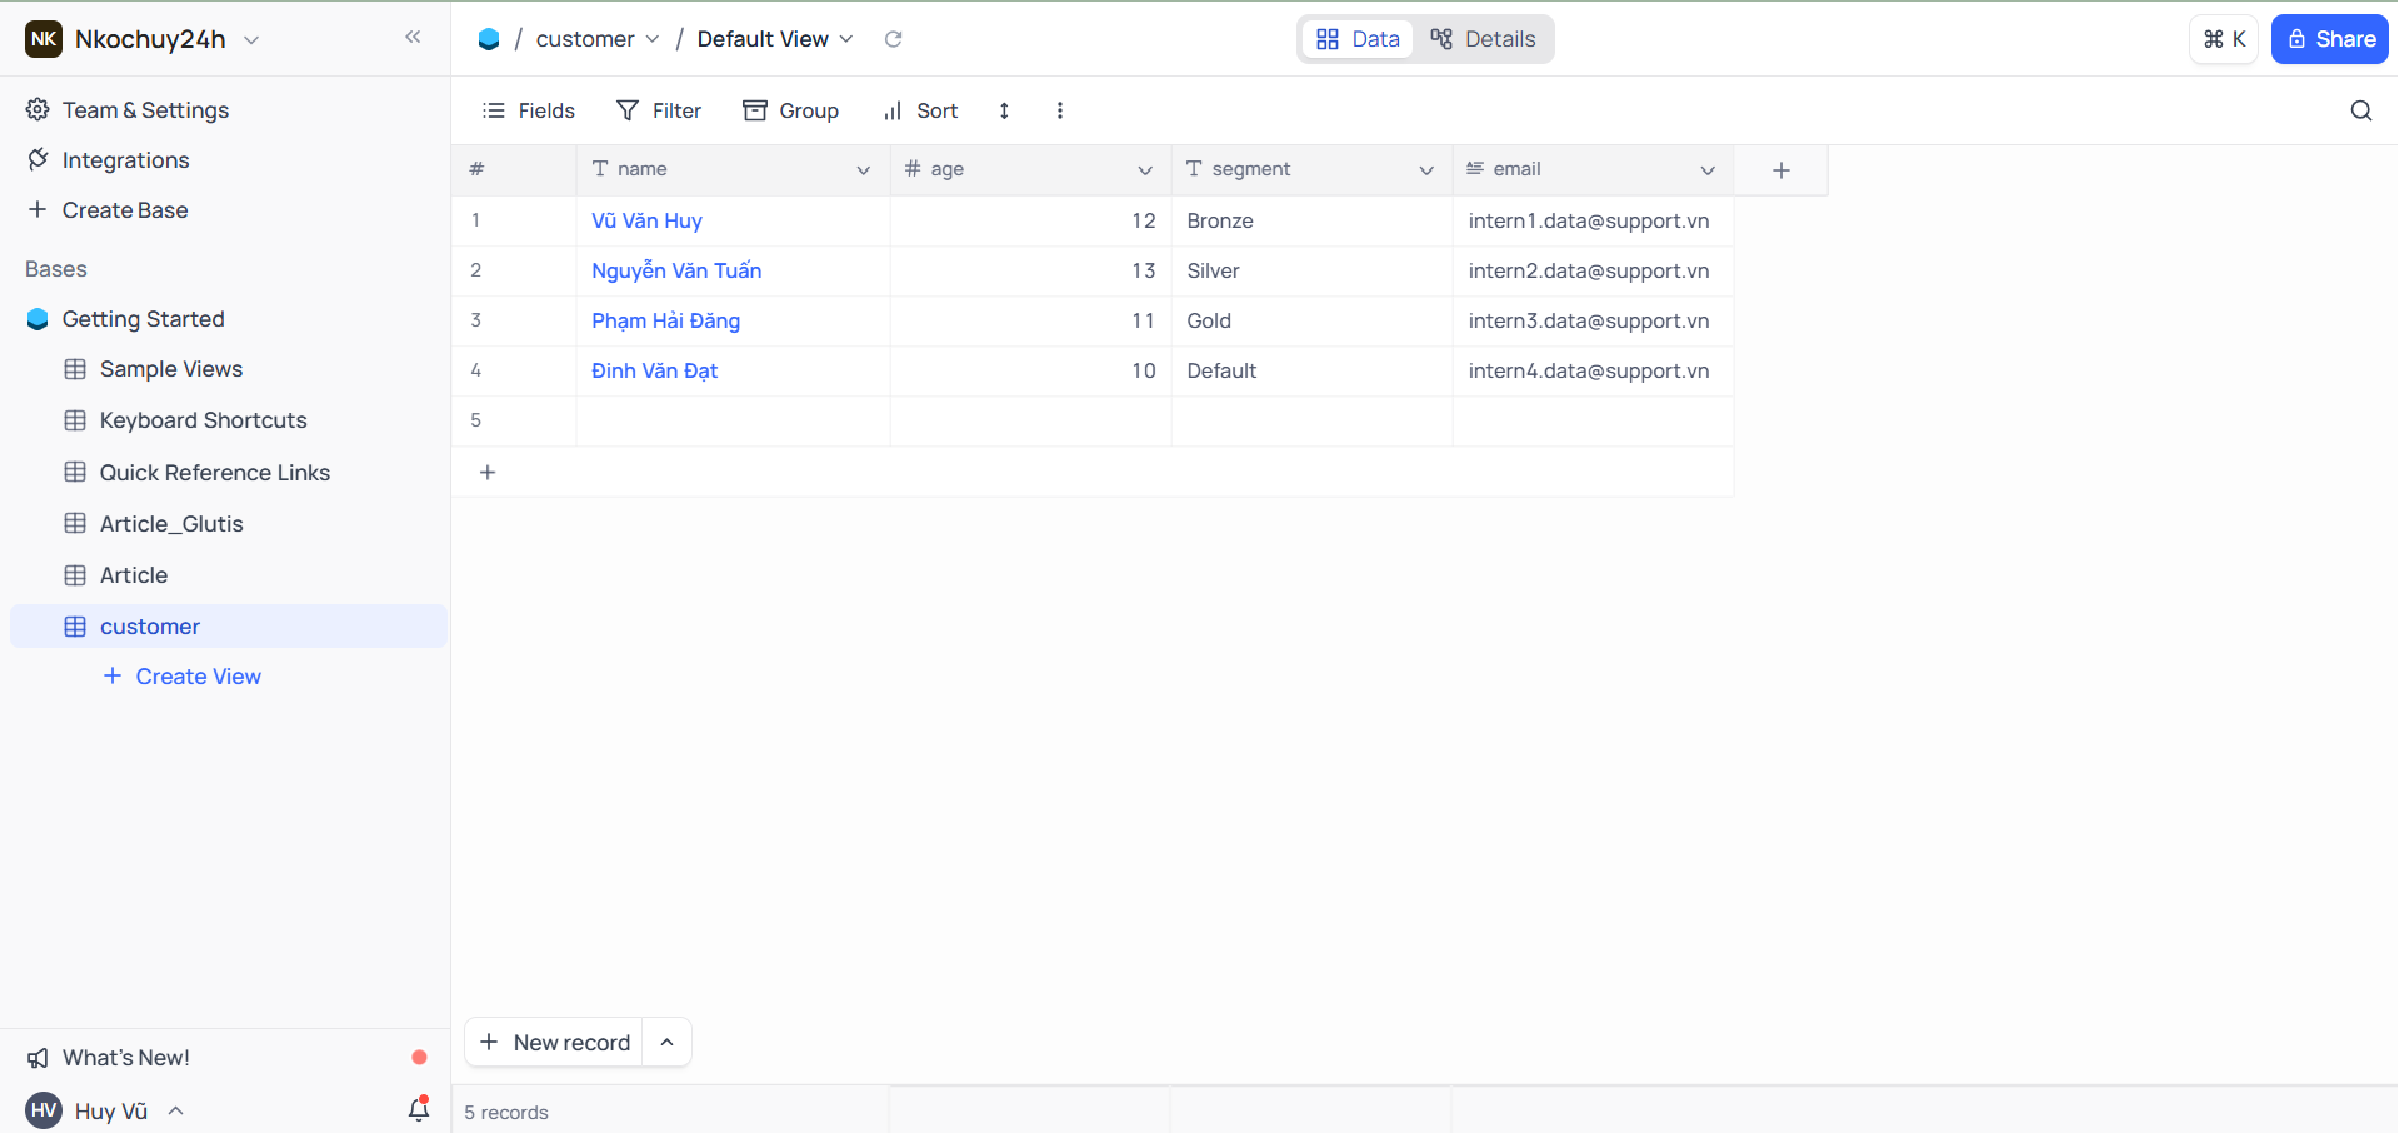
\includegraphics[width=1\linewidth]{Chap1-7/segment_db.pdf}
    \caption{Database chia phân loại khách hàng}
\end{figure}

Xây dựng workflow phân loại khách hàng dựa trên cấp độ thành viên:

\begin{figure}[htbp]
    \centering
    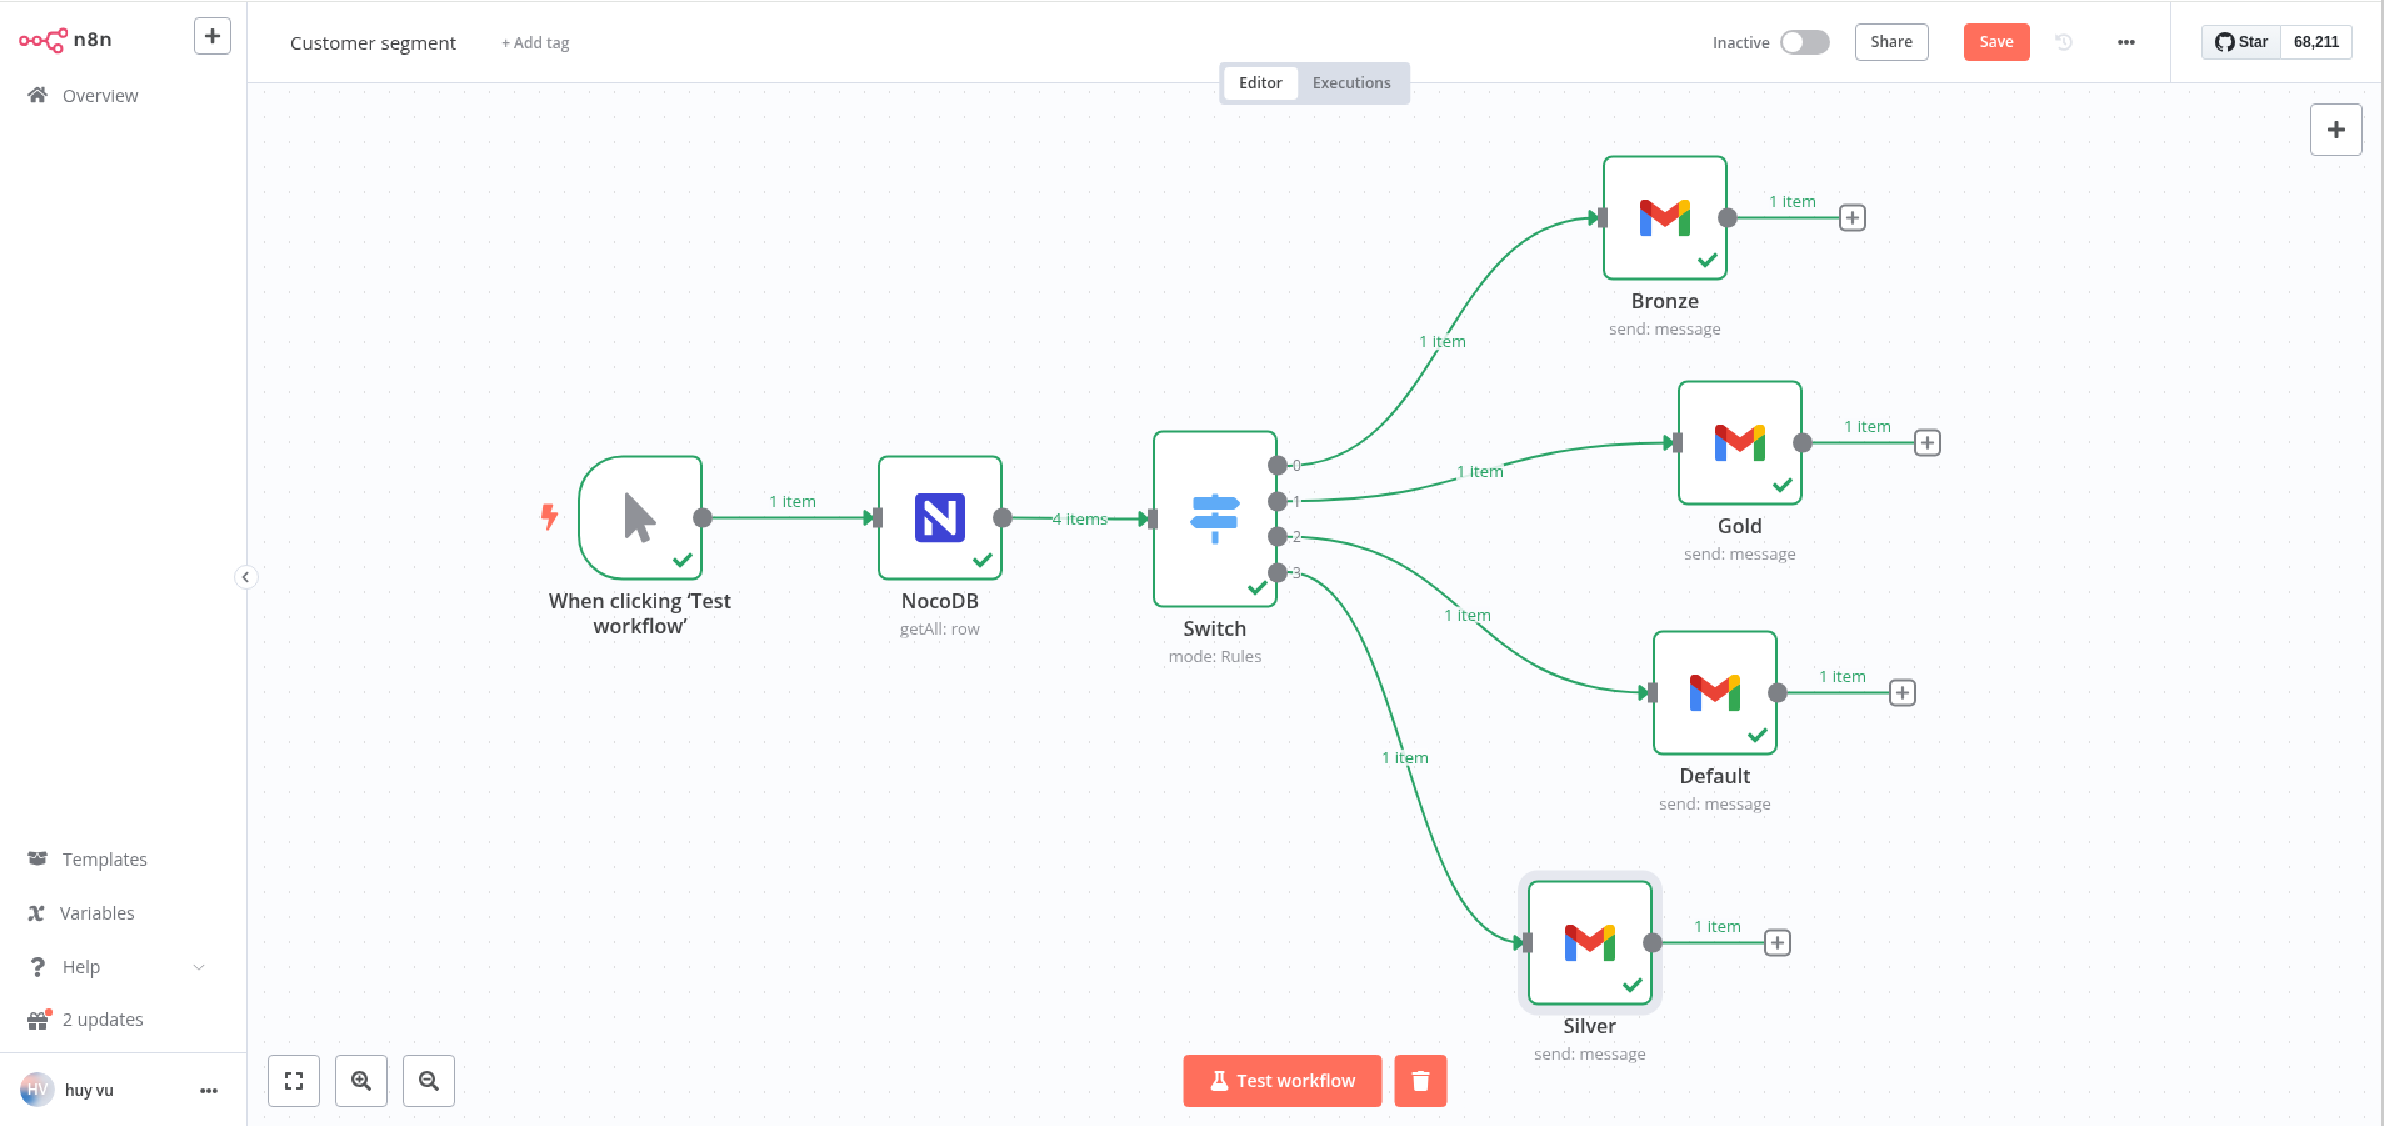
\includegraphics[width=1\linewidth]{Chap1-7/segment.pdf}
    \caption{Gửi email chăm sóc theo phân khúc khách hàng}
\end{figure}

Cấu hình Switch Node:
\begin{itemize}
  \item Value to Switch On: \texttt{\{\{\$json["membership\_level"]\}\}}
  \item Output 1: Name ``Bronze'', Value ``bronze''
  \item Output 2: Name ``Silver'', Value ``silver''
  \item Output 3: Name ``Gold'', Value ``gold''
  \item Default Output: For unmatched values
\end{itemize}

\subsection{Merge Node - Kết hợp dữ liệu từ nhiều nhánh}

Sau khi chia workflow thành nhiều nhánh với IF hoặc Switch, bạn thường cần kết hợp chúng lại để tiếp tục xử lý. Đây là lúc Merge Node phát huy tác dụng.

\subsubsection{Cách hoạt động của Merge Node}

Merge Node kết hợp dữ liệu từ nhiều nhánh thành một luồng duy nhất theo nhiều cách khác nhau.

\begin{figure}[htbp]
    \centering
    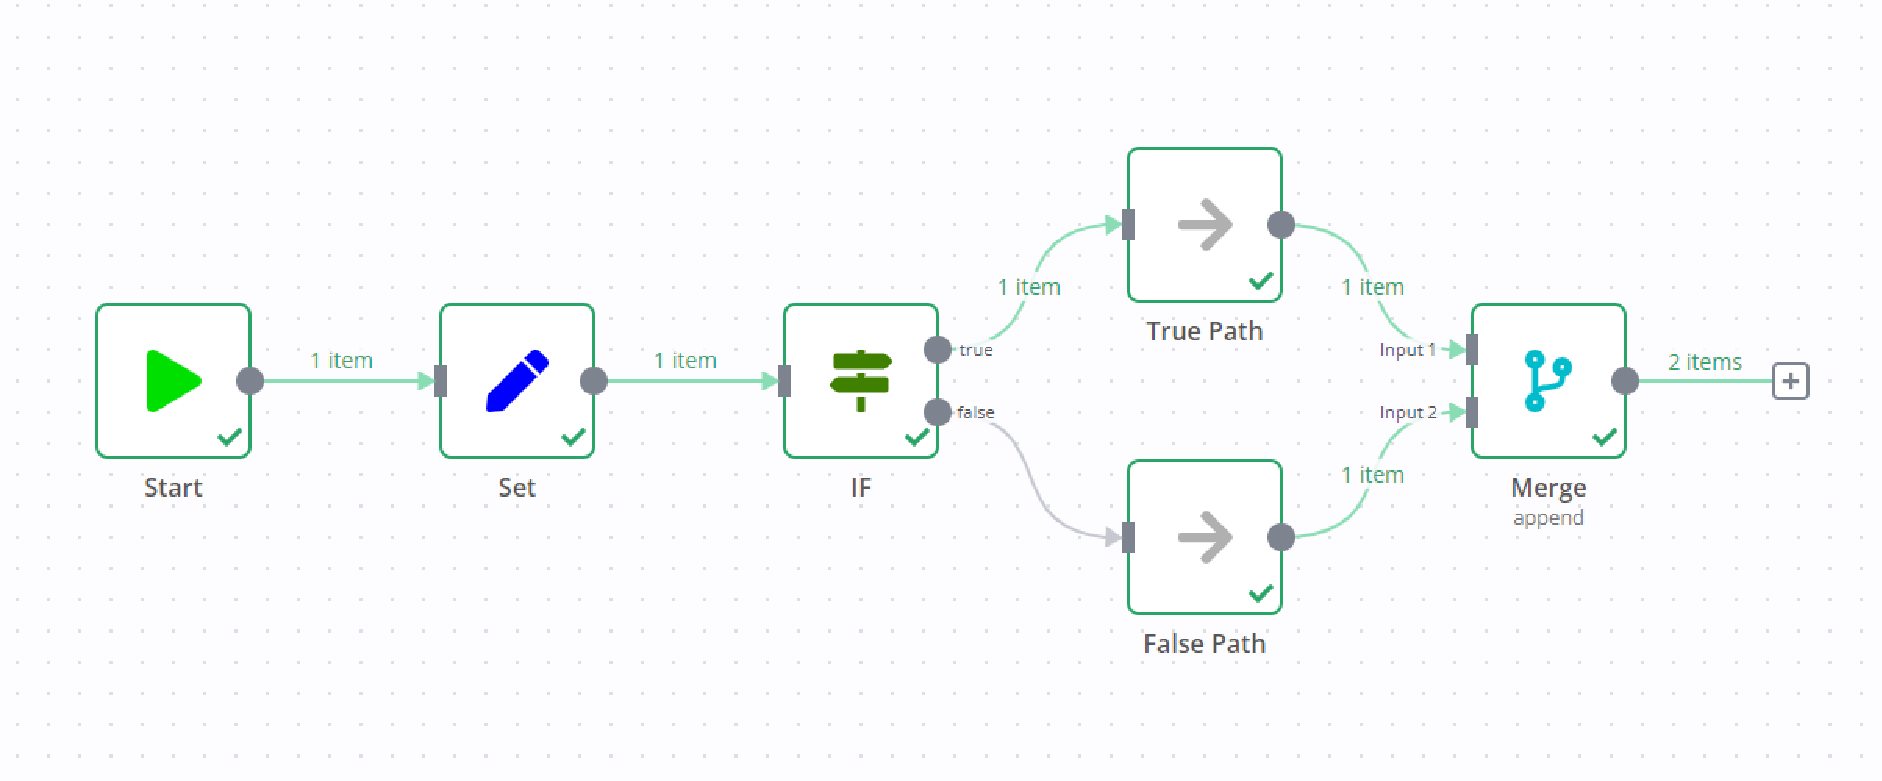
\includegraphics[width=1\linewidth]{Chap1-7/merge_node.pdf}
\end{figure} 

\subsubsection{Chế độ hoạt động của Merge Node}

\begin{enumerate}
  \item \textbf{Chế độ Append (Nối)}:
  \begin{itemize}
    \item Ghép các mục từ tất cả các đầu vào thành một mảng.
    \item Hữu ích khi bạn muốn xử lý tất cả các mục cùng một lúc.
  \end{itemize}

  \item \textbf{Chế độ Passthrough (Chuyển tiếp)}:
  \begin{itemize}
    \item Chuyển tiếp dữ liệu từ nút đầu tiên được kích hoạt.
    \item Hữu ích cho các tình huống ``race condition'' khi bạn chỉ muốn xử lý kết quả nhanh nhất.
  \end{itemize}

  \item \textbf{Chế độ Wait (Chờ đợi)}:
  \begin{itemize}
    \item Chờ tất cả các đầu vào trước khi xử lý.
    \item Có thể định cấu hình thêm để chỉ xử lý những đầu vào cụ thể.
  \end{itemize}
\end{enumerate}

\subsubsection{Ví dụ: Thu thập dữ liệu từ nhiều nguồn}

Thu thập dữ liệu sản phẩm từ nhiều API, sau đó tổng hợp thành một báo cáo:

\begin{figure}[htbp]
    \centering
    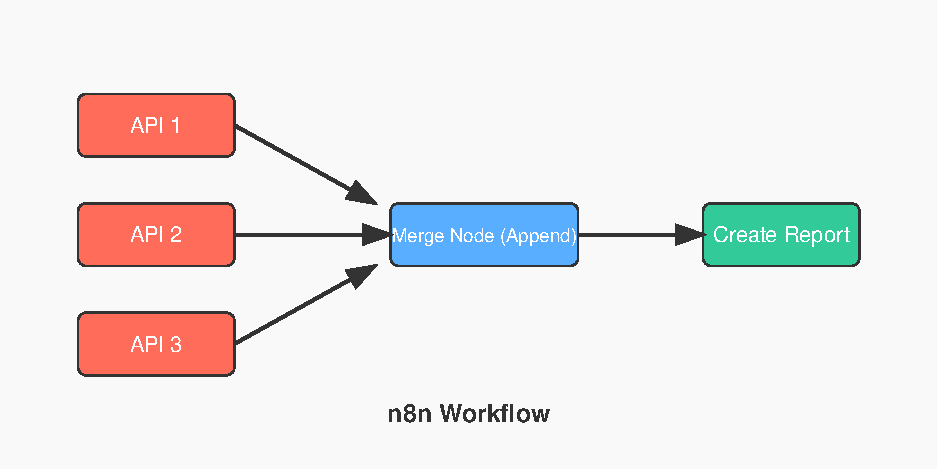
\includegraphics[width=1\linewidth]{Chap1-7/merge.pdf}
    % \caption{Caption}
\end{figure}

Cấu hình Merge Node:
\begin{itemize}
  \item Mode: Append
  \item Output format: Combine data from all inputs into a single array
\end{itemize}

Do n8n hoạt động theo nguyên tắc chạy các luồng từ trên xuống dưới, từ trái sang phải. Vì vậy sẽ không có 2 luồng rẽ nhánh mà cùng chạy và cho kết quả song song, Node merge này sẽ giúp ta làm điều đó. 


Ta lấy một ví dụ như này cho dễ hiểu: một API để truy xuất thông tin đơn hàng, API này cần 2 tham số là user\_id và order\_id được lấy từ bảng users và order. Ta có 2 node để lấy user\_id và order\_id 2 node này nếu trực tiếp đi vào node chứa api thì sẽ gây lỗi do node này chạy trước, node kia chạy sau. Lúc này ta sẽ cần node merger để tổng hợp kết quả từ 2 node đằng trước cùng lúc để truyền vào node chứa api sau đó.

\clearpage
\subsection{Kết hợp IF, Switch và Merge}

Các nút IF, Switch và Merge thường được sử dụng cùng nhau để tạo các workflow phức tạp.

\subsubsection{Ví dụ: Hệ thống xử lý đơn hàng}

Xây dựng workflow xử lý đơn hàng dựa trên tình trạng thanh toán và tồn kho:

\begin{figure}[htbp]
    \centering
    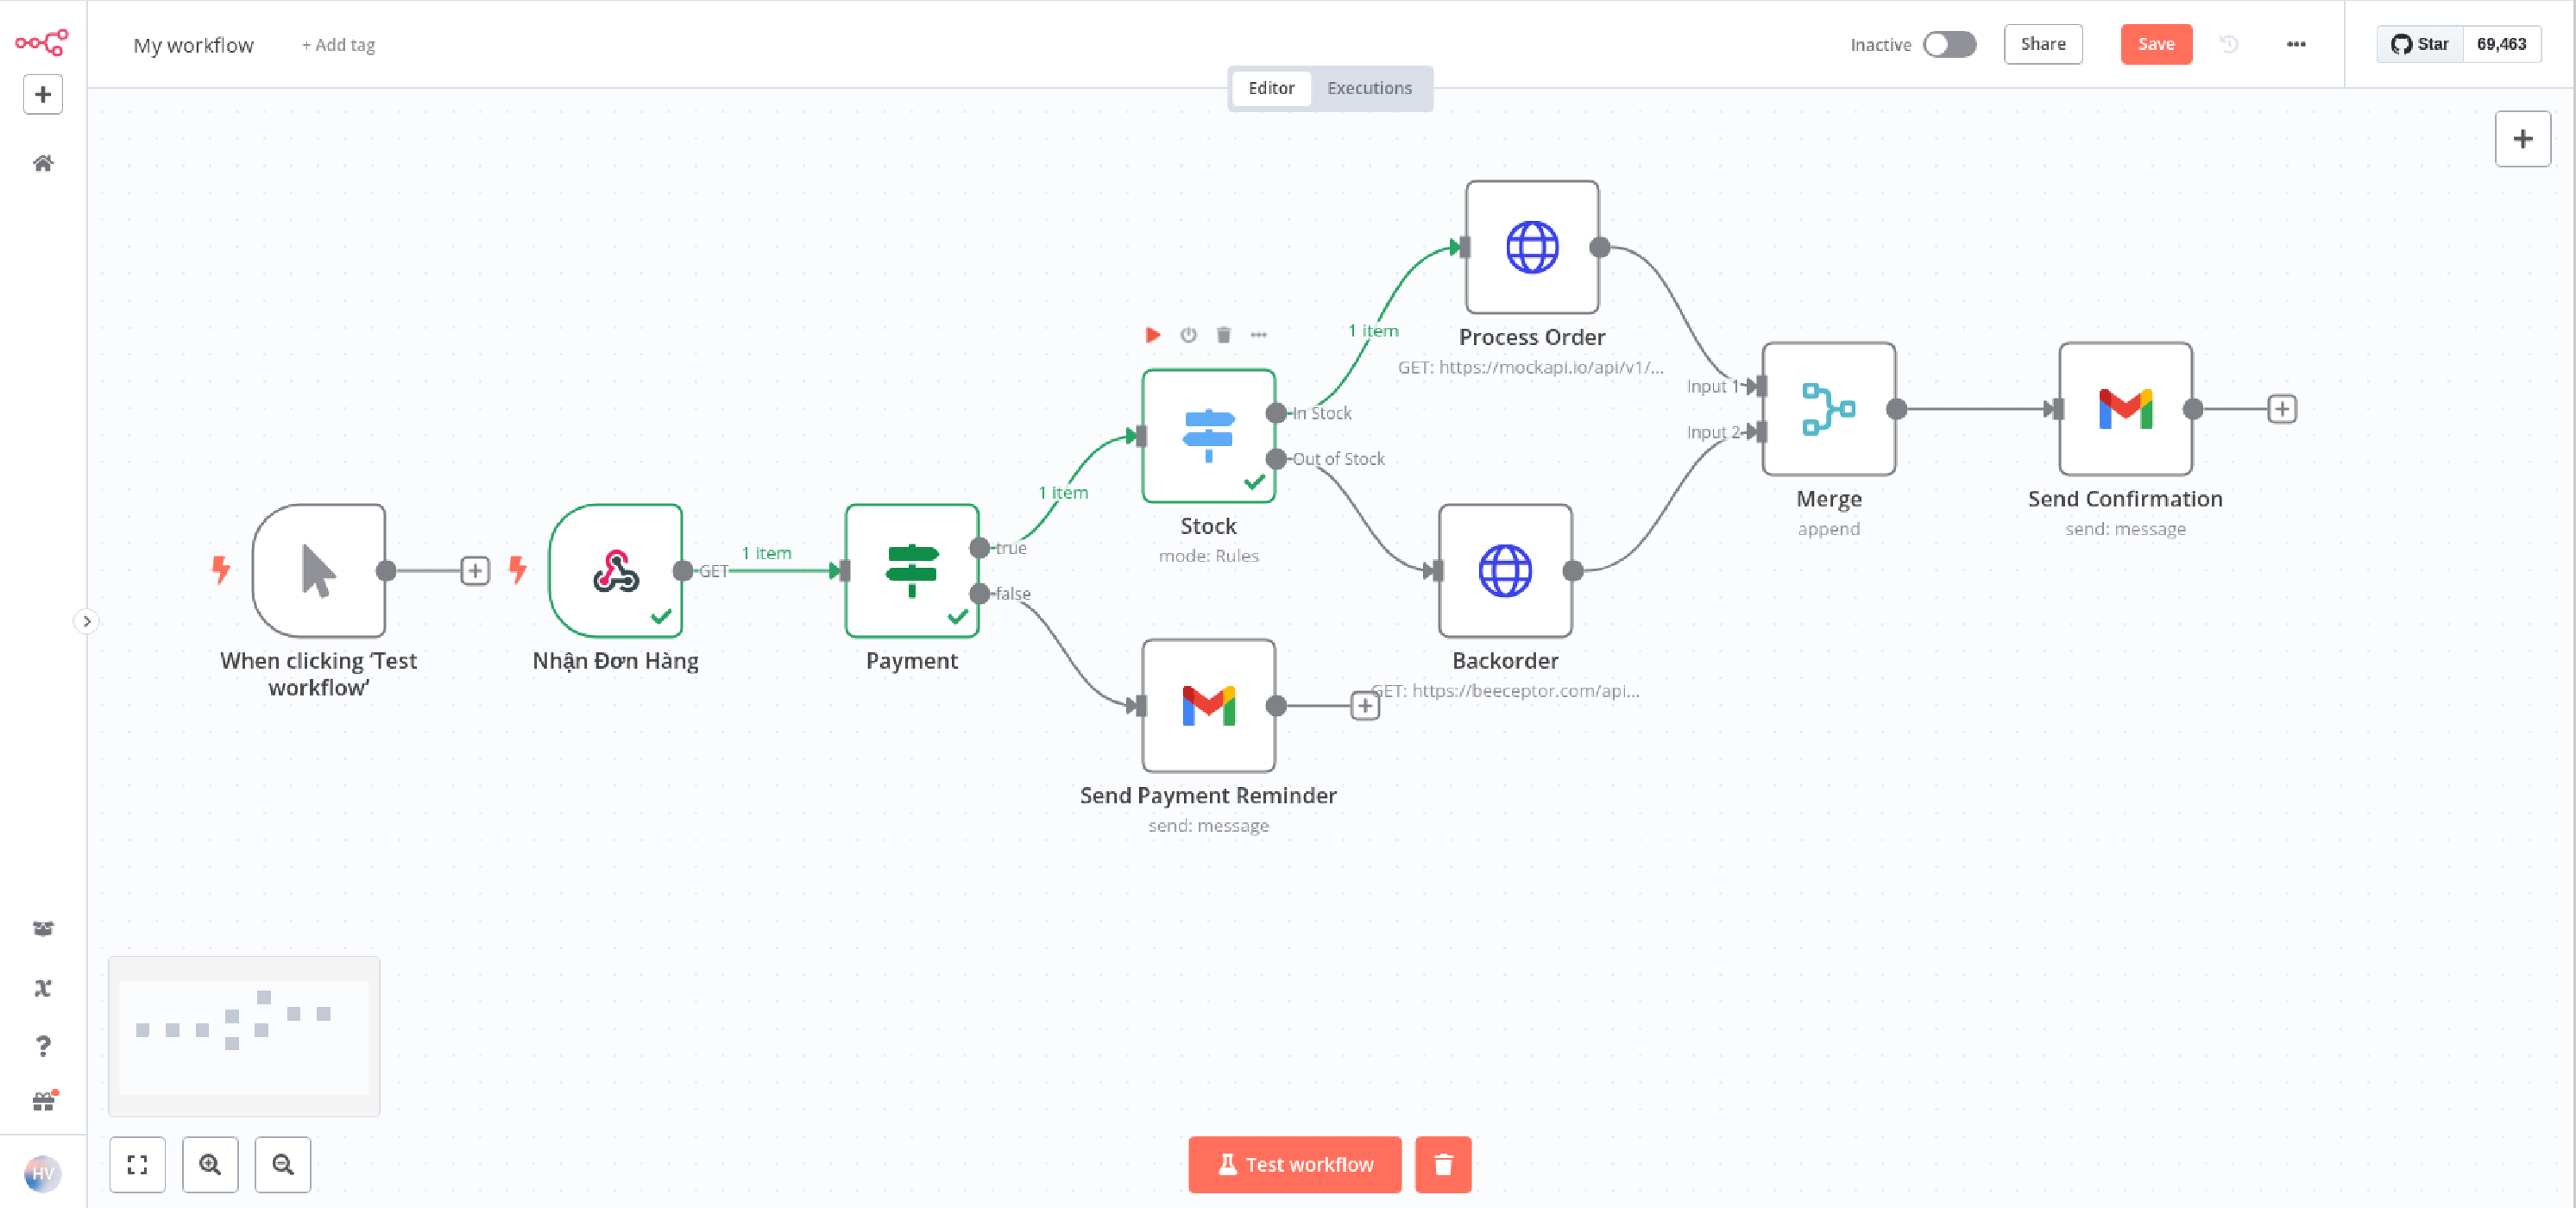
\includegraphics[width=1\linewidth]{Chap1-7/stock.pdf}
    % \caption{Caption}
    % \label{fig:enter-label}
\end{figure}

% \begin{verbatim}
% Order -> IF Node (Payment) -> [True] -> Switch Node (Stock) -> [In Stock] -> Process Order
%                            -> [False] -> Send Payment Reminder

%                                                            -> [Out of Stock] -> Backorder
                                                           
% Process Order -> 
% Backorder    -> Merge Node -> Send Confirmation
% \end{verbatim}

Cấu hình:
\begin{enumerate}
  \item IF Node:
  \begin{itemize}
    \item Điều kiện: \texttt{\{\{\$json["payment\_status"]\}\}} \texttt{equals} \texttt{"paid"}
  \end{itemize}

  \item Switch Node:
  \begin{itemize}
    \item Value: \texttt{\{\{\$json["stock\_status"]\}\}}
    \item Output 1: ``In Stock'', Value ``available''
    \item Output 2: ``Out of Stock'', Value ``unavailable''
  \end{itemize}

  \item Merge Node:
  \begin{itemize}
    \item Mode: Append
    \item Kết hợp cả đơn hàng xử lý thành công và đơn hàng chờ để gửi xác nhận.
  \end{itemize}
\end{enumerate}

\section{Vòng lặp For, While trong n8n}

\subsection{For Loop}

Trong lập trình truyền thống, vòng lặp là kỹ thuật căn bản giúp tự động hóa việc lặp đi lặp lại một hành động với dữ liệu.

Vòng lặp FOR: Lặp qua một tập hợp dữ liệu có số lượng xác định.
Ví dụ: lặp 10 lần, lặp qua danh sách 100 khách hàng.

Cấu trúc phổ biến:

\begin{verbatim}
for (khởi tạo; điều kiện; bước lặp) {
    // hành động
}
\end{verbatim}
Trong n8n, để lặp qua danh sách dữ liệu — tương tự vòng lặp FOR — chúng ta sử dụng node Split In Batches. Trước tiên, hãy học cách "chia để trị" dữ liệu. Trong n8n, node Split In Batches chính là công cụ đắc lực giúp bạn chia nhỏ dữ liệu thành từng phần, đảm bảo workflow vận hành mượt mà và dễ kiểm soát.

\subsubsection{Split In Batches hoạt động như thế nào?}

Hãy tưởng tượng bạn có một danh sách dài khách hàng cần xử lý. Thay vì dồn hết vào một lần — dễ quá tải, dễ lỗi — bạn chia thành từng nhóm nhỏ (batch) và xử lý từng nhóm một cách nhẹ nhàng.

\begin{figure}[htbp]
    \centering
    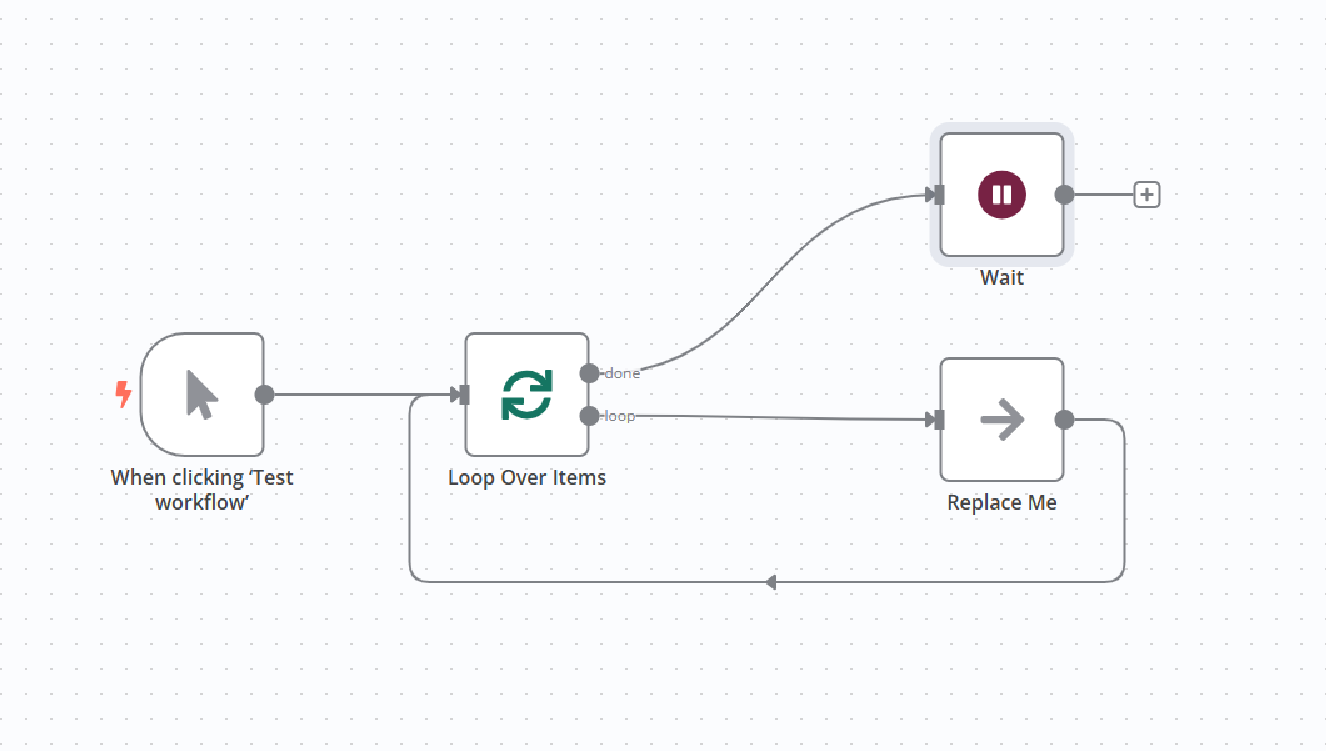
\includegraphics[width=1\linewidth]{Chap1-7/loop.pdf}
    \caption{Split In Batches}
\end{figure}

\subsubsection{Cấu hình Split In Batches}

\begin{enumerate}
  \item \textbf{Thêm Split In Batches vào workflow}:
  \begin{itemize}
    \item Tìm và thêm ``Split In Batches'' từ thư viện nút.
  \end{itemize}

  \item \textbf{Cấu hình kích thước batch}:
  \begin{itemize}
    \item Batch Size: Số lượng mục trong mỗi batch.
    \item Ví dụ: Nếu có 100 mục và batch size là 10, sẽ tạo ra 10 batch.
  \end{itemize}
\end{enumerate}

\textit{Mẹo: Chọn batch size phù hợp để tối ưu tốc độ mà không làm quá tải hệ thống.}

\subsubsection{Ví dụ: Xử lý danh sách khách hàng}

\begin{verbatim}
Database (1000 customers) -> Split In Batches (100) -> Process Each Batch
\end{verbatim}

\subsection{While Loop}
Vòng lặp WHILE: Lặp cho tới khi một điều kiện trở thành sai.
WHILE phù hợp với các tình huống không biết trước số lần lặp, như chờ API trả kết quả.

Cấu trúc:

\begin{verbatim}
while (điều kiện) {
    // hành động
}
\end{verbatim}


Khi học lập trình, chúng ta quen với các vòng lặp như FOR, WHILE, DO-WHILE, hay WHILE-DO. Tuy nhiên, trong n8n — một nền tảng no-code/low-code — không có sẵn một node While hay cấu hình vòng lặp trực tiếp trong một node khác. Không sao hết, thay vào đó, chúng ta hoàn toàn có thể mô phỏng một vòng lặp bằng cách tận dụng đường đi của các node.

\subsubsection{Cách hoạt động của While loop}   

Tận dụng kĩ năng lập trình, các kiến thức về while loop trong ngôn các ngôn ngữ lập trình. Ta sử dụng node điều kiện (ví dụ IF hoặc Switch) để kiểm tra điều kiện lặp, và nếu điều kiện đúng thì tiếp tục đi qua các node xử lý, rồi quay ngược lại node kiểm tra điều kiện. Nếu điều kiện sai thì dừng vòng lặp.

Ta xét workflow minh họa sau:

\begin{figure}[htbp]
    \centering
    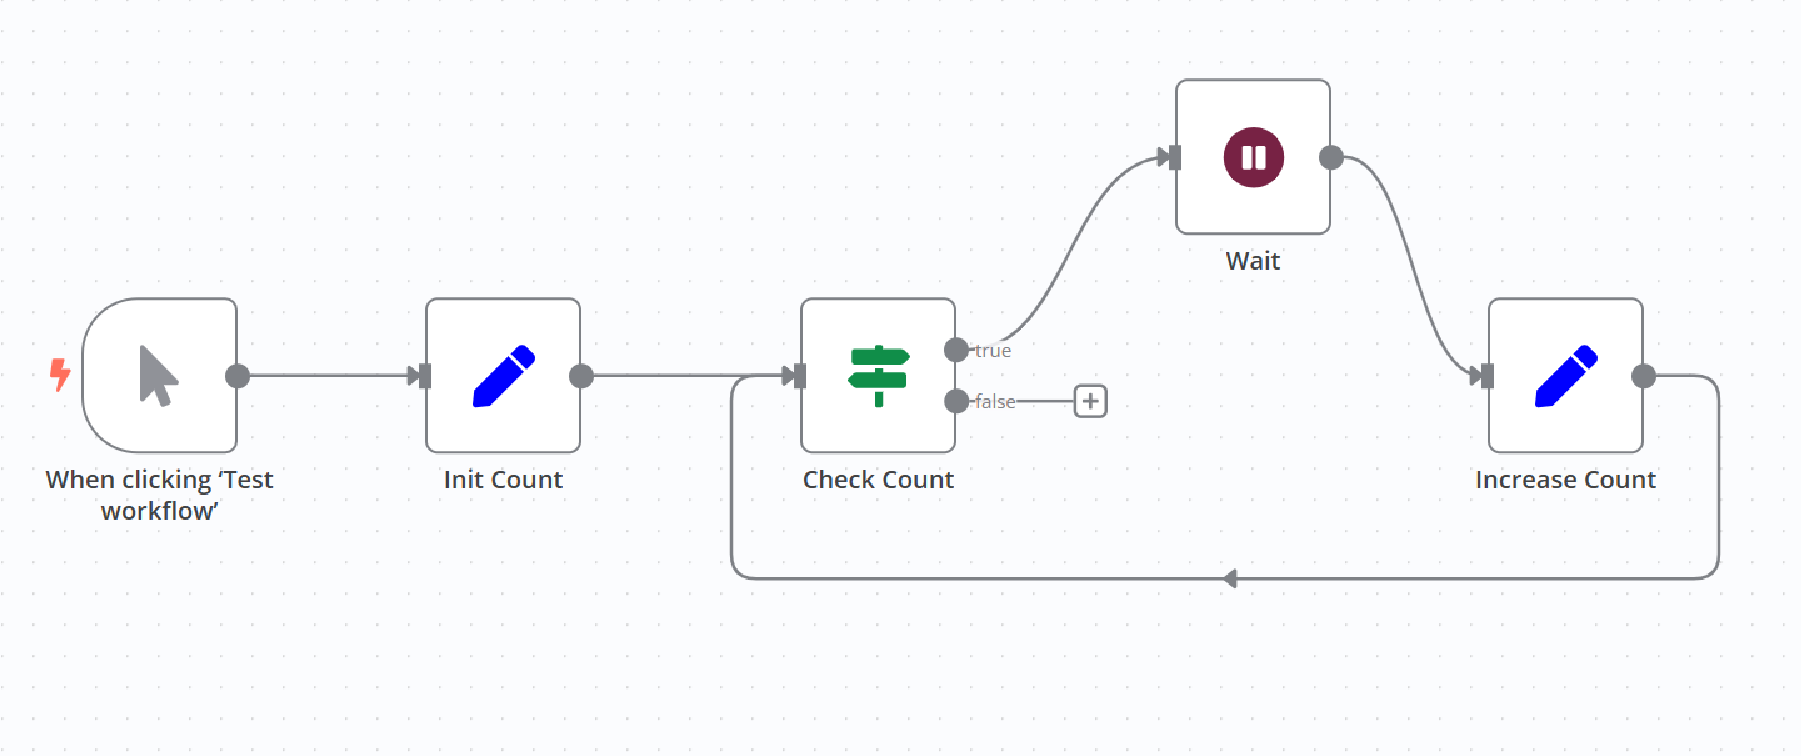
\includegraphics[width=1\linewidth]{Chap1-7/While-loop.pdf}
    \caption{Minh họa while loop}
\end{figure}
Mô tả:
\begin{itemize}
    \item When clicking 'Test workflow': Trigger khởi động workflow.

    \item Init Count: Thiết lập biến count = 0.

    \item Check Count: Kiểm tra nếu count < 5 thì trả về true, ngược lại false.

    \item Nếu true:
\begin{itemize}
    \item Wait: Dừng tạm workflow một khoảng thời gian (ví dụ 1s).

    \item Increase Count: Tăng giá trị count lên 1.

    \item Quay lại node Check Count để kiểm tra lại.

\end{itemize}
    \item Nếu false: workflow kết thúc.

\end{itemize}

Dù n8n không có node WHILE sẵn, nhưng bằng cách thiết kế luồng workflow hợp lý và kết hợp node IF, Wait, và các node xử lý logic khác, bạn hoàn toàn có thể tạo ra vòng lặp WHILE, FOR hay DO-WHILE.

\subsubsection{Ví dụ: Polling API cho đến khi nhận được kết quả}

\begin{verbatim}
While Node -> HTTP Request -> IF (Result Ready) 
 -> [True] -> Exit Loop
 -> [False] -> Wait 1s -> Back to While
\end{verbatim}

Cấu hình:
\begin{itemize}
  \item While Condition: \texttt{\{\{\$json["status"]\}\}} \texttt{not equals} \texttt{"completed"}
  \item HTTP Request: Kiểm tra trạng thái của một tác vụ dài.
  \item IF Node: Kiểm tra xem tác vụ đã hoàn thành chưa.
  \item Wait: Chờ 5 giây trước khi thử lại.
\end{itemize}

\subsection{Kỹ thuật nâng cao: Vòng lặp lồng nhau}

Trong một số trường hợp, bạn có thể cần các vòng lặp lồng nhau để xử lý dữ liệu phức tạp.

\subsubsection{Ví dụ: Xử lý dữ liệu đa cấp}

Xử lý danh sách khách hàng và đơn hàng của họ:

\begin{verbatim}
Database (Customers) -> For Each Customer -> Database (Orders) 

-> For Each Order -> Process Order
\end{verbatim}

Cấu hình:
\begin{enumerate}
  \item For Each Customer:
  \begin{itemize}
    \item Items: \texttt{\{\{\$json["customers"]\}\}}
  \end{itemize}
  
  \item Database (Orders):
  \begin{itemize}
    \item Query: Get orders for the current customer.
  \end{itemize}
  
  \item For Each Order:
  \begin{itemize}
    \item Items: \texttt{\{\{\$json["orders"]\}\}}
  \end{itemize}
  
  \item Process Order:
  \begin{itemize}
    \item Logic xử lý đơn hàng.
  \end{itemize}
\end{enumerate}


\textit{Bạn có thể lặp lồng nhau bao nhiêu tầng tùy ý, miễn workflow hợp lý và được kiểm soát tốt.}

\newpage
\section{Xử lý lỗi trong workflow}
Trong quá trình xây dựng workflow với n8n, lỗi là điều không thể tránh khỏi. Một workflow hoàn chỉnh không chỉ cần chạy đúng khi mọi thứ suôn sẻ mà còn phải biết xử lý tốt các tình huống ngoại lệ để đảm bảo hệ thống vận hành ổn định, giảm thiểu rủi ro gián đoạn.
\subsection{Error Workflow - Xử lý lỗi cơ bản}
\begin{figure}[htbp]
    \centering
    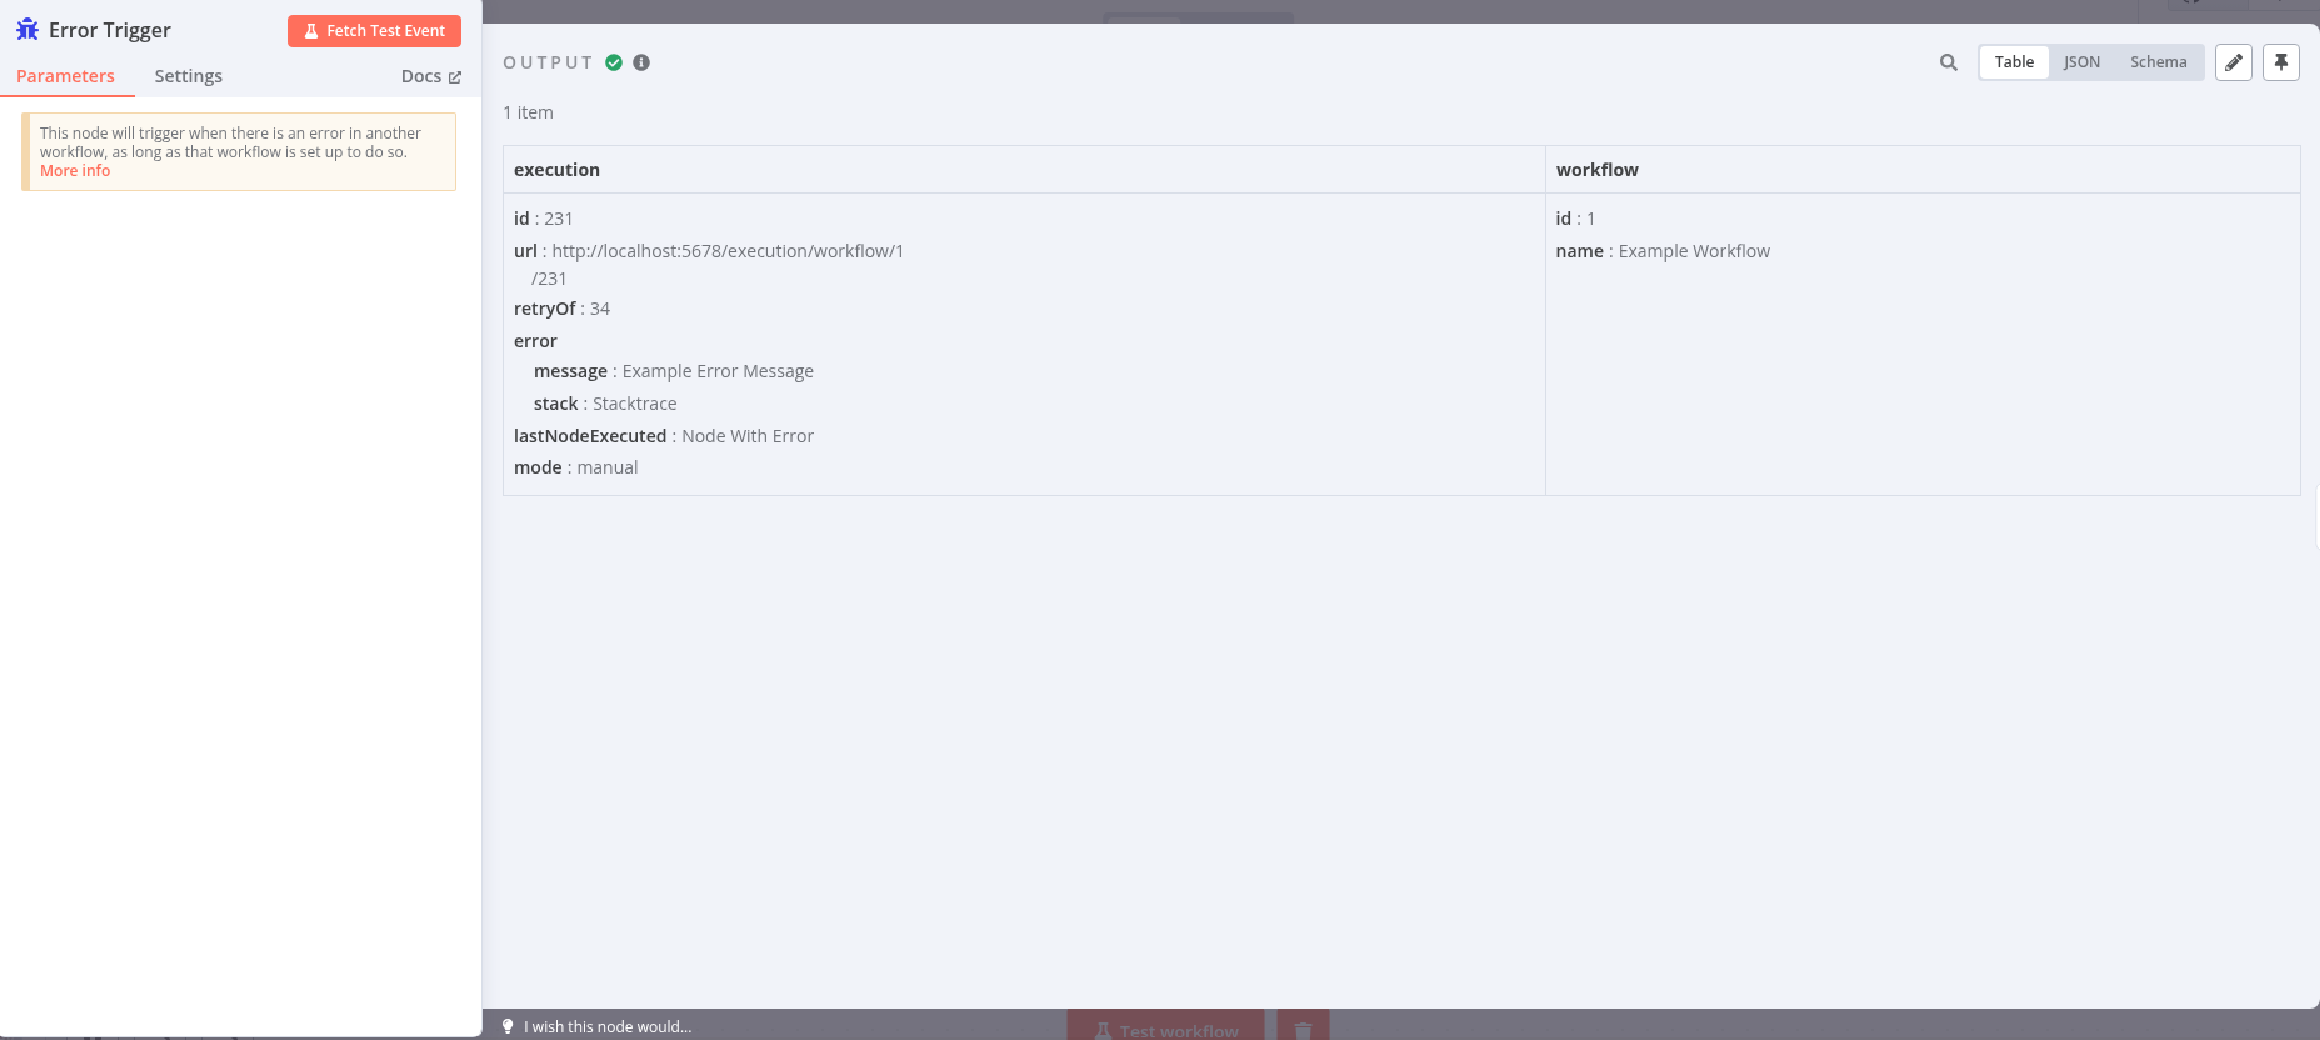
\includegraphics[width=1\linewidth]{Chap1-7/error_event.pdf}
    \caption{Khi một workflow lỗi nó sẽ trả về như này}
\end{figure}

$\rightarrow$ Để đảm bảo hệ thống hoạt động ổn định và có khả năng phục hồi, n8n cung cấp các cơ chế xử lý lỗi hiệu quả.

\subsubsection{Các loại lỗi phổ biến}

\begin{enumerate}
  \item Lỗi kết nối: Không thể kết nối đến API hoặc dịch vụ.
  \item Lỗi xác thực: Các vấn đề về xác thực hoặc ủy quyền.
  \item Lỗi dữ liệu: Dữ liệu không hợp lệ hoặc thiếu.
  \item Lỗi thời gian chờ: Các yêu cầu mất quá nhiều thời gian.
\end{enumerate}

\newpage

\subsubsection{Cấu hình Error Workflow}
\begin{figure}[htbp]
    \centering
    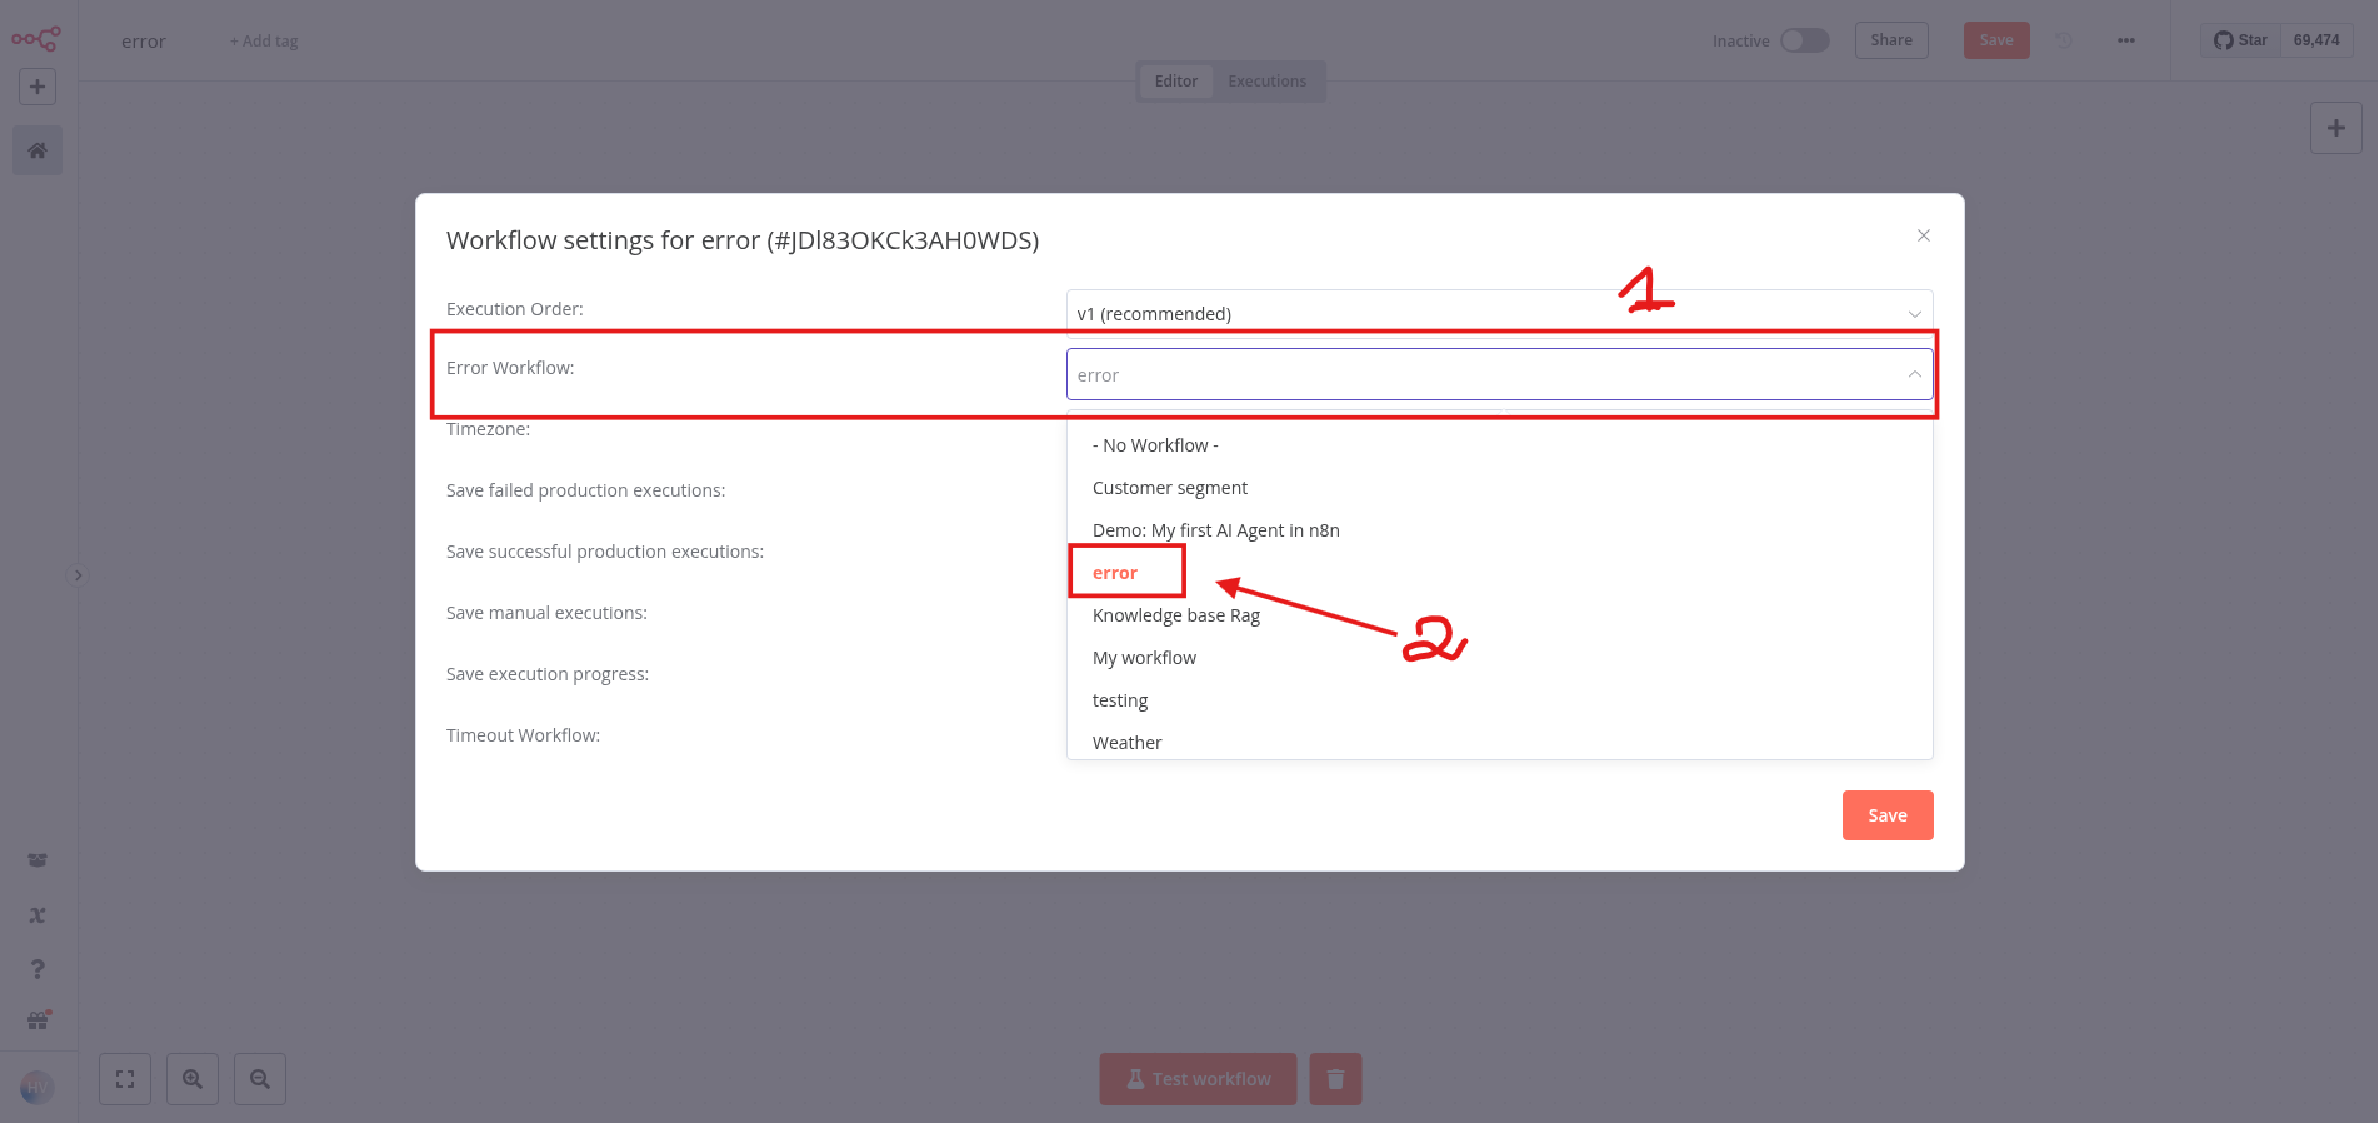
\includegraphics[width=1\linewidth]{Chap1-7/setting_error.pdf}
\end{figure}

N8N cho phép định nghĩa một Error Workflow - một workflow riêng biệt sẽ được kích hoạt khi workflow chính gặp lỗi.

\begin{enumerate}
  \item \textbf{Tạo Error Workflow}:
  \begin{itemize}
    \item Tạo một workflow mới để xử lý lỗi.
    \item Ví dụ: Gửi thông báo, ghi nhật ký lỗi, hoặc thực hiện các bước phục hồi.
  \end{itemize}

  \item \textbf{Kết nối với workflow chính}:
  \begin{itemize}
    \item Trong workflow chính, mở Settings > Error Workflow.
    \item Chọn Error Workflow đã tạo.
  \end{itemize}
\end{enumerate}

\subsection{Error Trigger Node}

Câu chuyện là khi mà workflow nó chạy ổn định mượt mà thì không sao trên thực tế thì lỗi rất nhiều (ae làm dev thì biết nè) chạy nó phải có lúc lỗi lúc không thường do nhiều nguyên nhân. Kiểu mấy tool như Airflow chạy cả năm không sao một ngày đùng phát có lỗi. Mà khi có lỗi thì workflow lỗi nó dùng và không chạy các node tiếp theo. 

$\Rightarrow$ \textit{Cần setup workflow để báo lỗi cho admin vào sửa}

\newpage

Error Trigger Node cho phép bạn bắt đầu một workflow dựa trên lỗi từ workflow khác.

\begin{figure}[htbp]
    \centering
    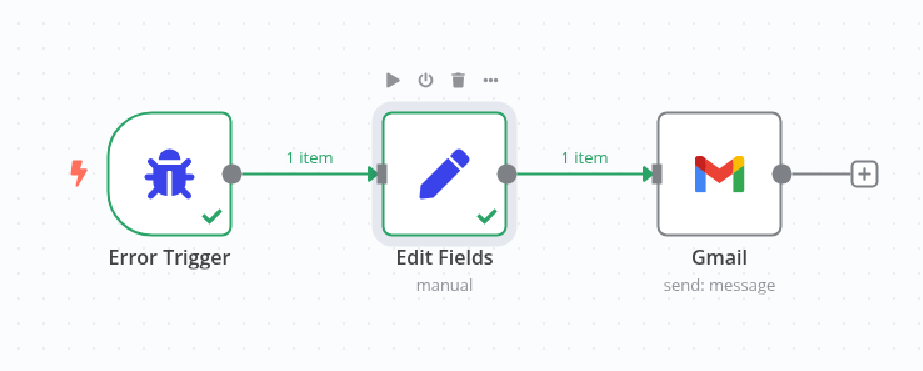
\includegraphics[width=1\linewidth]{Chap1-7/error.pdf}
\end{figure}

\subsubsection{Cấu hình Error Trigger}

\begin{figure}[htbp]
    \centering
    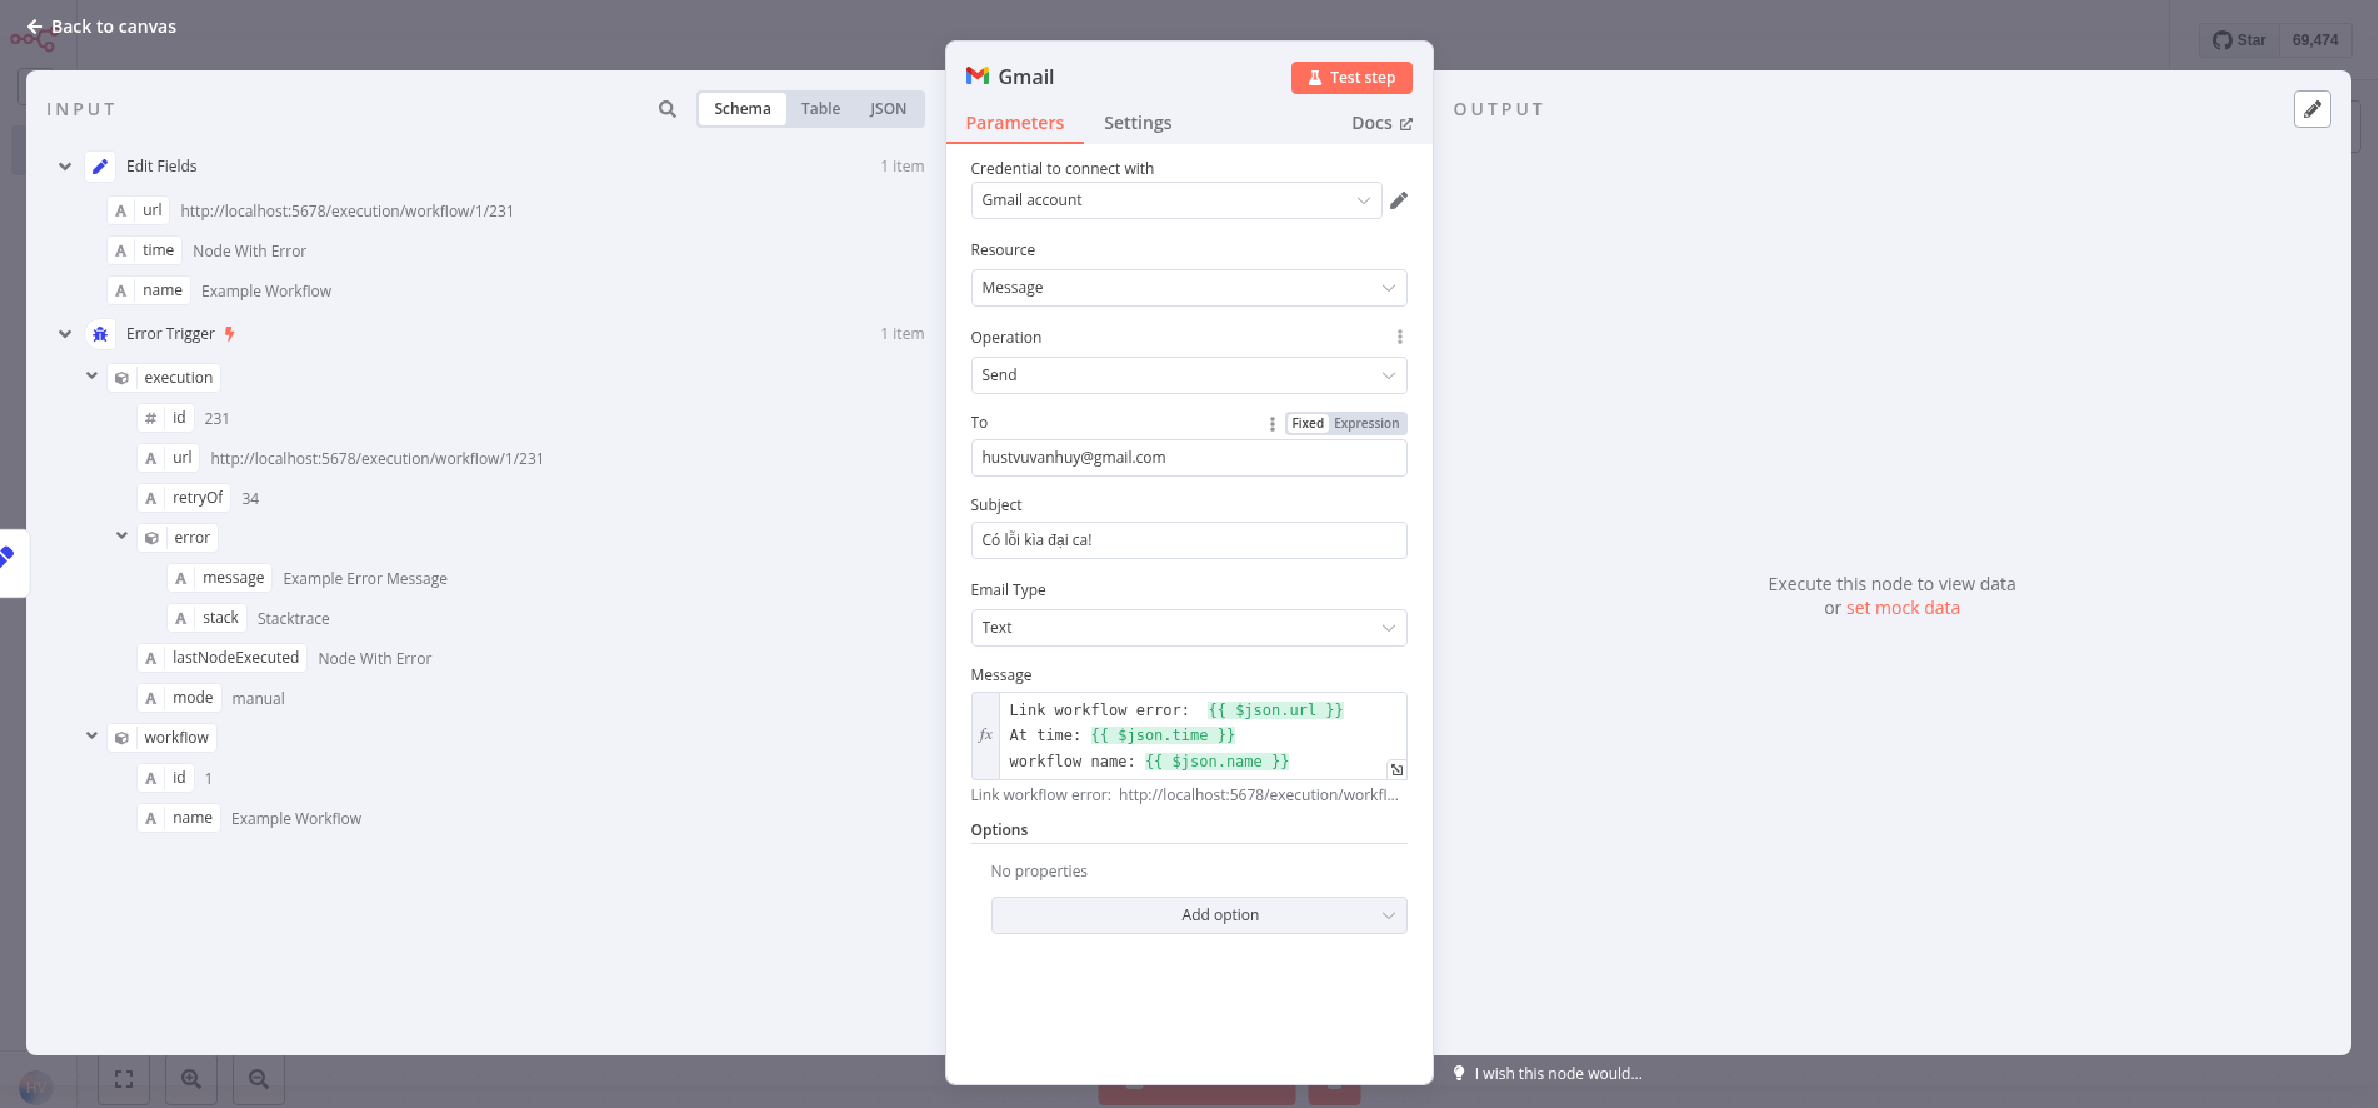
\includegraphics[width=1\linewidth]{Chap1-7/mess_error.pdf}
\end{figure}

\begin{enumerate}
  \item \textbf{Thêm Error Trigger vào Error Workflow}:
  \begin{itemize}
    \item Sử dụng ``Error Trigger'' làm nút bắt đầu.
  \end{itemize}

  \item \textbf{Thiết lập workflow cần theo dõi}:
  \begin{itemize}
    \item Chọn workflow cần được giám sát.
  \end{itemize}

  \item \textbf{Xử lý dữ liệu lỗi}:
  \begin{itemize}
    \item Truy cập thông tin lỗi thông qua \texttt{\{\{\$json["error"]\}\}}.
    \item Truy cập workflow gốc thông qua \texttt{\{\{\$json["workflow"]\}\}}.
    \item Hoàn toàn có thể lưu các lỗi vào sheet để dễ dàng theo dõi.
  \end{itemize}
\end{enumerate}


\subsection{Try/Catch trong n8n}

n8n không có cú pháp Try/Catch giống như các ngôn ngữ lập trình, nhưng bạn có thể mô phỏng hành vi này.

\subsubsection{Cách thực hiện Try/Catch}

Sử dụng kết hợp IF Node, Error Trigger và Function Node:

\begin{verbatim}
-> Function (Try) -> IF (Success) -> [True] -> Tiếp tục workflow
                  -> [False] -> Function (Catch) -> Xử lý lỗi
\end{verbatim}

Cấu hình:
\begin{enumerate}
  \item Function (Try):
  \begin{verbatim}
  try {
    // Mã có thể gây lỗi
    const result = await $items(0).json.riskyOperation();
    return { success: true, data: result };
  } catch (error) {
    return { success: false, error: error.message };
  }
  \end{verbatim}

  \item IF Node:
  \begin{itemize}
    \item Điều kiện: \texttt{\{\{\$json["success"]\}\}} \texttt{equals} \texttt{true}
  \end{itemize}

  \item Function (Catch):
  \begin{verbatim}
  // Xử lý lỗi
  return { error_handled: true, message: "Đã xử lý lỗi: " + $items(0).json.error };
  \end{verbatim}
\end{enumerate}

\newpage
\subsection{Retry khi gặp lỗi}

Thêm khả năng thử lại cho các hoạt động không ổn định như các yêu cầu API.

\subsubsection{Sử dụng vòng lặp và điều kiện để thử lại}

\begin{verbatim}
While Loop -> HTTP Request -> IF (Success) 
 -> [True] -> Exit Loop
 -> [False] -> Function (Retry Logic) -> Back to While
\end{verbatim}

Cấu hình:
\begin{enumerate}
  \item Function (Retry Logic):
  \begin{verbatim}
  // Tăng bộ đếm thử lại
  const retryCount = $items(0).json.retryCount || 0;
  const maxRetries = 3;
  
  if (retryCount < maxRetries) {
    return { retryCount: retryCount + 1, retry: true };
  } else {
    return { retryCount: retryCount, retry: false, error: "Đã vượt quá số lần thử lại" };
  }
  \end{verbatim}

  \item While loop:
  \begin{itemize}
    \item Điều kiện: \texttt{\{\{\$json["retry"]\}\}} \texttt{equals} \texttt{true}
  \end{itemize}
\end{enumerate}

\subsubsection{Ví dụ: Gọi API không ổn định}

\begin{verbatim}
Set (retryCount:0) -> While (retryCount<3) -> HTTP Request -> IF (Success)
 -> [True] -> Exit 
 -> [False] -> Wait -> Increment retryCount
\end{verbatim}
\subsection{Ghi nhật ký và giám sát}

Việc ghi nhật ký đầy đủ là quan trọng để giám sát và gỡ lỗi workflow.

\subsubsection{Thêm ghi nhật ký vào workflow}

\begin{enumerate}
  \item \textbf{Function Node để ghi nhật ký}:
  \begin{verbatim}
  // Ghi nhật ký với dấu thời gian
  const log = {
    timestamp: new Date().toISOString(),
    step: "Processing Customer Data",
    data: $items(0).json
  };
  
  // Truyền cả dữ liệu gốc và thông tin nhật ký
  return { ...item[0].json, log };
  \end{verbatim}

  \item \textbf{Tích hợp với hệ thống giám sát}:
  \begin{itemize}
    \item Gửi nhật ký đến Slack, email, hoặc hệ thống giám sát.
    \item Lưu trữ nhật ký trong cơ sở dữ liệu để phân tích sau.
  \end{itemize}
\end{enumerate}

\subsubsection{Ví dụ: Workflow có khả năng phục hồi đầy đủ}

\begin{verbatim}
Trigger -> 
  Function (Log Start) -> 
    Try Process -> 
      IF (Success) -> 
        [True] -> Function (Log Success) -> Continue
        [False] -> Function (Log Error) -> Error Handling -> Retry Logic
\end{verbatim}

\section{Tổng kết}

Trong chương này, chúng ta đã tìm hiểu về:

\begin{enumerate}
  \item Nút điều kiện (IF, Switch) để tạo các luồng xử lý động dựa trên dữ liệu.
  \item Merge Node để kết hợp dữ liệu từ nhiều nhánh.
  \item Vòng lặp (Each Item, For Each, While) để xử lý nhiều mục dữ liệu.
  \item Xử lý lỗi để tạo các workflow có khả năng phục hồi.
\end{enumerate}

Việc kết hợp các kỹ thuật này sẽ cho phép bạn xây dựng các workflow phức tạp và mạnh mẽ, có thể xử lý các tình huống thực tế đa dạng.

\newpage
\section{Bài tập thực hành}

\begin{enumerate}
  \item Tạo một workflow sử dụng IF Node để phân loại email dựa trên nội dung.
  \item Xây dựng một workflow sử dụng For Each để gửi thông báo tùy chỉnh cho từng thành viên trong nhóm.
  \item Tạo một Error Workflow để thông báo và ghi nhật ký khi workflow chính gặp sự cố.
\end{enumerate}

%%% Chương 6
\chapter{Xử lý dữ liệu nâng cao trong n8n}

\section{Function Node \& Code Snippets}

\subsection{Giới thiệu Function Node}

Function Node là một trong những công cụ mạnh mẽ nhất của n8n, cho phép bạn viết mã JavaScript để xử lý dữ liệu theo cách tùy chỉnh. Function Node đặc biệt hữu ích khi các node có sẵn không đáp ứng được nhu cầu cụ thể của bạn.

\subsubsection{Cấu trúc cơ bản của Function Node}

\begin{lstlisting}[language=JavaScript]
items = items.map(item => {
  return item;
});
return items;
\end{lstlisting}

\subsubsection{Ví dụ 1: Chuyển đổi định dạng dữ liệu}

Giả sử bạn nhận được danh sách sản phẩm từ một API và cần chuyển đổi định dạng để phù hợp với hệ thống của bạn:

\begin{lstlisting}[language=JavaScript]
items = items.map(item => {
  const newItem = {
    productId: item.json.id,
    name: item.json.product_name,
    price: parseFloat(item.json.price),
    inStock: item.json.stock_quantity > 0,
    categories: item.json.category.split(',').map(cat => cat.trim())
  };
  
  item.json = newItem;
  
  return item;
});

return items;
\end{lstlisting}

\subsubsection{Ví dụ 2: Lọc và tổng hợp dữ liệu}
- Lọc sản phẩm có giá trên 100 và còn hàng

- Tính tổng giá trị hàng tồn kho

- Trả về một item mới chứa thông tin tổng hợp

\begin{lstlisting}[language=JavaScript]
const filteredItems = items.filter(item => 
  item.json.price > 100 && item.json.inStock === true
);

let totalValue = 0;
filteredItems.forEach(item => {
  totalValue += item.json.price * item.json.stock_quantity;
});

return [{
  json: {
    filteredProducts: filteredItems.map(item => item.json),
    totalProducts: filteredItems.length,
    totalInventoryValue: totalValue,
    generatedAt: new Date().toISOString()
  }
}];
\end{lstlisting}

\subsection{Các mẹo và thủ thuật với Function Node}

\subsubsection{Sử dụng thư viện bên ngoài}

n8n cho phép bạn sử dụng nhiều thư viện JavaScript phổ biến:

- Sử dụng thư viện moment để xử lý thời gian

\begin{lstlisting}[language=JavaScript]
const moment = require('moment');

items = items.map(item => {
  // convert timestamp 
  item.json.createdAtFormatted = moment(item.json.created_at).format('DD/MM/YYYY HH:mm');
  
  // Calc day to now
  item.json.daysSinceCreation = moment().diff(moment(item.json.created_at), 'days');
  
  return item;
});

return items;
\end{lstlisting}

\subsubsection{Xử lý lỗi trong Function Node}

\begin{lstlisting}[language=JavaScript]
items = items.map(item => {
  try {
    if (typeof item.json.data === 'string') {
      item.json.data = JSON.parse(item.json.data);
    }
  } catch (error) {
    // Process error
    item.json.data = { error: "data not valid" };
    item.json.parseError = error.message;
  }
  
  return item;
});

return items;
\end{lstlisting}

\subsubsection{Kết hợp dữ liệu từ nhiều node}

Giả sử node 1 trả về thông tin sản phẩm và node 2 trả về thông tin giá

\begin{lstlisting}[language=JavaScript]
const productsData = $node["HTTP Request"].json.products;
const pricesData = $node["HTTP Request1"].json.prices;

// combind
const combinedData = productsData.map(product => {
  const price = pricesData.find(p => p.product_id === product.id);
  
  return {
    ...product,
    price: price ? price.amount : 0,
    currency: price ? price.currency : 'USD'
  };
});

return [{ json: { combinedData } }];
\end{lstlisting}

\section{Kết nối database: MySQL, PostgreSQL, MongoDB, Nocodb}

\subsection{Thiết lập kết nối cơ sở dữ liệu}

n8n cung cấp nhiều node để kết nối với các loại cơ sở dữ liệu phổ biến. Dưới đây là hướng dẫn thiết lập và sử dụng các kết nối này.

\subsubsection{Kết nối MySQL}

\paragraph{Thiết lập Credentials:}
\begin{itemize}
    \item Trong n8n, vào phần Credentials và chọn "New Credentials"
    \item Chọn loại "MySQL"
    \item Nhập thông tin kết nối: Host, Port, Database, User, Password
    \item Lưu lại credentials
\end{itemize}

\paragraph{Ví dụ: Tự động đồng bộ dữ liệu từ API vào MySQL}

Workflow:
\begin{itemize}
    \item HTTP Request Node để lấy dữ liệu từ API
    \item Function Node để xử lý và chuẩn bị dữ liệu
    \item MySQL Node để lưu dữ liệu
\end{itemize}

\begin{lstlisting}[language=JavaScript]
items = items.map(item => {
  return {
    json: {
      operation: "insert",
      table: "products",
      data: {
        name: item.json.name,
        sku: item.json.sku,
        price: item.json.price,
        stock: item.json.available_quantity,
        updated_at: new Date().toISOString()
      }
    }
  };
});

return items;
\end{lstlisting}

Cấu hình MySQL Node:
\begin{itemize}
    \item Chọn credentials đã tạo
    \item Operation: Execute Query
    \item Query tự động được tạo dựa trên dữ liệu từ Function Node
\end{itemize}

\subsubsection{Kết nối PostgreSQL}

Tương tự như MySQL, nhưng với một số đặc điểm riêng:

\paragraph{Ví dụ: Thực hiện thao tác UPSERT trong PostgreSQL}

\begin{lstlisting}[language=JavaScript]
items = items.map(item => {
  return {
    json: {
      query: `
        INSERT INTO customers (email, name, phone, last_order_date)
        VALUES ($1, $2, $3, $4)
        ON CONFLICT (email) 
        DO UPDATE SET 
          name = $2,
          phone = $3,
          last_order_date = $4,
          updated_at = NOW()
      `,
      values: [
        item.json.email,
        item.json.name,
        item.json.phone,
        item.json.order_date
      ]
    }
  };
});

return items;
\end{lstlisting}

\subsubsection{Kết nối MongoDB}

MongoDB là cơ sở dữ liệu NoSQL phổ biến và n8n cũng hỗ trợ tốt:

\paragraph{Ví dụ: Tìm kiếm và cập nhật dữ liệu trong MongoDB}

Workflow:
\begin{itemize}
    \item Trigger Node (ví dụ: Webhook)
    \item MongoDB Node để tìm document
    \item Function Node để xử lý
    \item MongoDB Node thứ hai để cập nhật
\end{itemize}

Cấu hình MongoDB Node (Tìm kiếm):
\begin{itemize}
    \item Operation: Find
    \item Collection: orders
    \item Options: Thiết lập query để tìm đơn hàng theo ID
\end{itemize}
Giả sử data từ MongoDB chứa thông tin đơn hàng
Function Node:
\begin{lstlisting}[language=JavaScript]
items = items.map(item => {
  const order = item.json;
  
  let totalValue = 0;
  order.items.forEach(product => {
    totalValue += product.price * product.quantity;
  });
  
  return {
    json: {
      updateOne: {
        filter: { _id: order._id },
        update: {
          $set: {
            total_value: totalValue,
            shipping_status: "ready_to_ship",
            updated_at: new Date()
          }
        }
      }
    }
  };
});

return items;
\end{lstlisting}

\subsubsection{Kết nối NocoDB}

NocoDB là một giải pháp mã nguồn mở biến cơ sở dữ liệu thành Airtable-like. n8n có thể kết nối với NocoDB qua API:

\paragraph{Thiết lập Credentials NocoDB:}
\begin{itemize}
    \item Tạo API token trong NocoDB
    \item Trong n8n, tạo credentials loại "API Key Auth"
    \item Nhập API token vào trường "API Key Value"
\end{itemize}

\paragraph{Ví dụ: Đồng bộ dữ liệu từ CRM vào NocoDB}

HTTP Request Node (lấy dữ liệu từ CRM):
\begin{itemize}
    \item Method: GET
    \item URL: https://your-crm-api.com/contacts
    \item Authentication: Chọn credentials phù hợp
\end{itemize}


Function Node (chuẩn bị dữ liệu):Chuyển đổi từ định dạng CRM sang định dạng NocoDB
\begin{lstlisting}[language=JavaScript]
items = items.map(contact => {
  return {
    json: {
      Name: `${contact.json.first_name} ${contact.json.last_name}`,
      Email: contact.json.email,
      Phone: contact.json.phone,
      Company: contact.json.company,
      LastContact: contact.json.last_contacted_at,
      Tags: contact.json.tags.join(', ')
    }
  };
});

return items;
\end{lstlisting}

HTTP Request Node (gửi vào NocoDB):
\begin{itemize}
    \item Method: POST
    \item URL: https://your-nocodb.com/api/v1/tables/YOUR\_TABLE\_ID/records
    \item Headers: xc-auth: YOUR\_API\_TOKEN
    \item Body: Item Binary => json
\end{itemize}

\subsection{Các kỹ thuật Database nâng cao}

\subsubsection{Sử dụng Transaction}

Với các cơ sở dữ liệu hỗ trợ transaction như MySQL và PostgreSQL:

\begin{lstlisting}[language=JavaScript]
return [
  {
    json: {
      query: "BEGIN"
    }
  },
  {
    json: {
      query: "INSERT INTO orders (customer_id, total) VALUES ($1, $2) RETURNING id",
      values: [customerId, total]
    }
  },
  {
    json: {
      __nextNode: "Function Node"
    }
  },
  {
    json: {
      query: "COMMIT"
    }
  }
];
\end{lstlisting}

Function Node để xử lý order\_id:
\begin{lstlisting}[language=JavaScript]
const orderId = items[0].json.id;

return orderItems.map(item => {
  return {
    json: {
      query: "INSERT INTO order_items (order_id, product_id, quantity, price) VALUES ($1, $2, $3, $4)",
      values: [orderId, item.product_id, item.quantity, item.price]
    }
  };
});
\end{lstlisting}
\subsubsection{Thực hiện truy vấn phức tạp}

\begin{lstlisting}[language=JavaScript]
return [
  {
    json: {
      query: `
        SELECT 
          products.id, products.name, products.price,
          categories.name AS category,
          COUNT(order_items.id) AS times_ordered
        FROM 
          products
        LEFT JOIN 
          product_categories ON products.id = product_categories.product_id
        LEFT JOIN 
          categories ON product_categories.category_id = categories.id
        LEFT JOIN 
          order_items ON products.id = order_items.product_id
        WHERE 
          products.active = 1
        GROUP BY 
          products.id, categories.id
        ORDER BY 
          times_ordered DESC
        LIMIT 20
      `
    }
  }
];
\end{lstlisting}

\section{Làm việc với API nâng cao (OAuth, Auth Token)}

\subsection{Xác thực OAuth trong n8n}

OAuth là giao thức xác thực phổ biến cho các API hiện đại. n8n hỗ trợ nhiều dịch vụ OAuth như Google, Facebook, Twitter, và nhiều dịch vụ khác.

\subsubsection{Thiết lập OAuth 2.0 credentials}

\begin{enumerate}
    \item Đăng ký ứng dụng với nhà cung cấp dịch vụ (Google, Facebook, v.v.)
    \item Nhận Client ID và Client Secret
    \item Trong n8n, tạo credentials mới loại OAuth2 API
    \item Nhập thông tin:
    \begin{itemize}
        \item Client ID và Client Secret
        \item Authorization URL
        \item Token URL
        \item Scope cần thiết
        \item Authentication: Header (thường là mặc định)
    \end{itemize}
\end{enumerate}

\subsubsection{Ví dụ: Tích hợp với Google Drive}

Workflow:
\begin{itemize}
    \item Trigger Node (ví dụ: Webhook)
    \item Google Drive Node để tải file
\end{itemize}

Google Drive Node:
\begin{itemize}
    \item Operation: Download
    \item File ID: ID của file trong Google Drive (có thể lấy từ URL)
\end{itemize}

\subsubsection{Ví dụ: Tích hợp với Salesforce qua OAuth}

Workflow:
\begin{itemize}
    \item Cron Node (chạy hàng ngày)
    \item Salesforce Node để lấy danh sách các khách hàng mới
    \item Function Node để chuyển đổi dữ liệu
    \item Send Email Node để gửi báo cáo
\end{itemize}

Salesforce Node:
\begin{itemize}
    \item Operation: SOQL Query
    \item Query: SELECT Id, Name, Email, Phone, CreatedDate FROM Contact WHERE CreatedDate = TODAY
\end{itemize}

Function Node: Định dạng dữ liệu để gửi email
\begin{lstlisting}[language=JavaScript]
const contacts = items.map(item => item.json);

const emailContent = `
<h2>New customer (${new Date().toLocaleDateString()})</h2>
<table border="1" cellpadding="5">
  <tr>
    <th>Name</th>
    <th>Email</th>
    <th>phone</th>
  </tr>
  ${contacts.map(contact => `
    <tr>
      <td>${contact.Name}</td>
      <td>${contact.Email}</td>
      <td>${contact.Phone || 'N/A'}</td>
    </tr>
  `).join('')}
</table>
<p>Sum: ${contacts.length} new customer</p>
`;

return [
  {
    json: {
      to: "your-email@example.com",
      subject: `report ${new Date().toLocaleDateString()}`,
      html: emailContent
    }
  }
];
\end{lstlisting}

\subsection{Làm việc với API sử dụng Token Authentication}

Nhiều API sử dụng token authentication đơn giản hơn OAuth.

\subsubsection{Thiết lập Auth Token credentials}

\begin{enumerate}
    \item Trong n8n, tạo credentials mới loại "API Key Auth" hoặc "Bearer Token Auth"
    \item Nhập API key hoặc token từ dịch vụ
    \item Chọn vị trí chèn token (thường là Header)
    \item Nếu cần, tùy chỉnh tên trường header (ví dụ: "Authorization" hoặc "X-API-Key")
\end{enumerate}

\subsubsection{Ví dụ: Tích hợp với GitHub API}

Workflow:
\begin{itemize}
    \item Webhook Node (để nhận sự kiện từ ngoài)
    \item HTTP Request Node để gọi GitHub API
    \item Function Node để xử lý response
    \item Send Email Node để thông báo
\end{itemize}

HTTP Request Node:
\begin{itemize}
    \item Method: POST
    \item URL: https://api.github.com/repos/\{owner\}/\{repo\}/issues
    \item Authentication: Chọn Bearer Token Auth credentials
\end{itemize}
Body:
\begin{lstlisting}[language=JSON]
{
  "title": "Issue ",
  "body": "Report by webhook",
  "labels": ["bug", "automated"]
}
\end{lstlisting}

\subsubsection{Ví dụ: Refresh Token tự động}

Một số API yêu cầu làm mới token định kỳ. Dưới đây là cách thiết lập workflow để tự động làm mới token:

Workflow:
\begin{itemize}
    \item Cron Node (chạy định kỳ, ví dụ: mỗi 50 phút nếu token hết hạn sau 1 giờ)
    \item HTTP Request Node để làm mới token
    \item Function Node để lưu token mới
\end{itemize}

HTTP Request Node:
\begin{itemize}
    \item Method: POST
    \item URL: https://api.service.com/oauth/token
\end{itemize}

Body:
\begin{lstlisting}[language=JSON]
{
  "grant_type": "refresh_token",
  "refresh_token": "{{$node["Get Stored Credentials"].json.refresh_token}}",
  "client_id": "your_client_id",
  "client_secret": "your_client_secret"
}
\end{lstlisting}

Function Node:
% \begin{lstlisting}[language=JavaScript]
% // Lưu token mới vào n8n
% const tokenData = items[0].json;

% // Bạn có thể lưu vào database hoặc sử dụng n8n variables
% // Hoặc cập nhật credentials

% return [
%   {
%     json: {
%       success: true,
%       message: "Token đã được làm mới",
%       expires_at: new Date(Date.now() + tokenData.expires_in * 1000).toISOString()
%     }
%   }
% ];
% \end{lstlisting}

\subsection{Xây dựng Middleware API với n8n}

n8n có thể được sử dụng như một middleware giữa các API khác nhau, cho phép bạn:
\begin{itemize}
    \item Chuyển đổi định dạng dữ liệu
    \item Kết hợp dữ liệu từ nhiều nguồn
    \item Thêm xác thực và kiểm soát truy cập
\end{itemize}

\subsubsection{Ví dụ: Middleware cho CRM và Marketing Automation}

Workflow:
\begin{itemize}
    \item Webhook Node (endpoint API của bạn)
    \item Switch Node để định tuyến request
    \item HTTP Request Node để gọi API của CRM
    \item HTTP Request Node khác để gọi API của Marketing Platform
    \item Function Node để kết hợp kết quả
    \item Respond to Webhook Node để trả về kết quả
\end{itemize}

Function Node:
\begin{lstlisting}[language=JavaScript]
const crmData = $node["HTTP Request"].json;
const marketingData = $node["HTTP Request1"].json;

const combinedData = {
  contact: {
    id: crmData.id,
    name: crmData.name,
    email: crmData.email,
    phone: crmData.phone
  },
  marketing: {
    campaigns: marketingData.campaigns,
    lastOpened: marketingData.last_activity,
    clickRate: marketingData.statistics.click_rate
  },
  summary: {
    totalSpent: crmData.total_purchases,
    totalEmails: marketingData.statistics.total_emails,
    engagementScore: (marketingData.statistics.open_rate * 0.4 + 
                      marketingData.statistics.click_rate * 0.6).toFixed(2)
  }
};

return [{ json: combinedData }];
\end{lstlisting}

\section{Các kỹ thuật xử lý dữ liệu nâng cao}

\subsection{Xử lý dữ liệu batch và pagination}

Khi làm việc với lượng lớn dữ liệu, pagination là kỹ thuật quan trọng:

\begin{lstlisting}[language=JavaScript]
let allData = [];
let page = 1;
let hasMore = true;

while (hasMore) {
  // call API 
  const response = await httpRequest({
    url: `https://api.example.com/items?page=${page}`,
    headers: { 'Authorization': 'Bearer your_token' }
  });
  
  allData = [...allData, ...response.data.items];
  
  hasMore = response.data.has_more;
  page++;
  
  if (page > 100) break;
}

return [{ json: { items: allData } }];
\end{lstlisting}

\subsection{Xử lý dữ liệu song song với Wait node}

n8n cho phép xử lý song song nhiều luồng dữ liệu, sau đó kết hợp kết quả:

Workflow:
\begin{itemize}
    \item Split In Batches Node để chia nhỏ dữ liệu
    \item Nhiều nhánh xử lý song song
    \item Wait Node để đợi tất cả hoàn thành
    \item Merge Node để kết hợp kết quả
\end{itemize}

\subsection{Mã hóa và bảo mật dữ liệu}
Mã hóa dữ liệu nhạy cảm. Thay thế dữ liệu nhạy cảm bằng dữ liệu đã mã hóa
\begin{lstlisting}[language=JavaScript]
const crypto = require('crypto');

items = items.map(item => {
  const key = crypto.scryptSync('password', 'salt', 24);
  const iv = Buffer.alloc(16, 0);
  
  const cipher = crypto.createCipheriv('aes-192-cbc', key, iv);
  let encrypted = cipher.update(item.json.creditCard, 'utf8', 'hex');
  encrypted += cipher.final('hex');
  
  item.json.creditCard = encrypted;
  
  return item;
});

return items;
\end{lstlisting}

\section{Các ví dụ workflow hoàn chỉnh}

\subsection{Workflow 1: Hệ thống theo dõi kho hàng tự động}

\subsubsection{Mục tiêu:} Tự động cập nhật kho hàng từ nhiều nguồn (database, API), gửi thông báo khi sản phẩm sắp hết hàng, và tạo báo cáo hàng tuần.

\subsubsection{Các node chính:}
\begin{enumerate}
    \item Cron Node (chạy hàng ngày)
    \item MySQL Node (lấy dữ liệu kho hàng)
    \item HTTP Request Node (lấy dữ liệu từ API nhà cung cấp)
    \item Function Node (kết hợp và phân tích dữ liệu)
    \item IF Node (kiểm tra sản phẩm sắp hết hàng)
    \item Send Email Node (gửi cảnh báo)
    \item Google Sheets Node (lưu dữ liệu cho báo cáo)
\end{enumerate}

\subsection{Workflow 2: Tích hợp CRM và Marketing Automation}

\subsubsection{Mục tiêu:} Tự động đồng bộ hóa khách hàng giữa CRM và hệ thống email marketing, phân đoạn khách hàng dựa trên hành vi, và tự động gửi email cá nhân hóa.

\subsubsection{Các node chính:}
\begin{enumerate}
    \item Webhook Node (kích hoạt khi có khách hàng mới trong CRM)
    \item HTTP Request Node (lấy chi tiết khách hàng từ CRM API)
    \item Function Node (xử lý và phân đoạn khách hàng)
    \item IF Node (định tuyến dựa trên phân đoạn)
    \item HTTP Request Node 
\end{enumerate}

%% Chương 7
\chapter{AI trong n8n - Xu hướng và ứng dụng}
Chào mừng bạn đến với một trong những phần thú vị nhất của n8n: tích hợp trí tuệ nhân tạo! Nếu bạn nghĩ rằng tự động hóa quy trình công việc đã tuyệt vời rồi, thì việc thêm AI vào n8n sẽ đưa mọi thứ lên một tầm cao mới.


\section{Giới thiệu về Large Language Model}
Mô hình ngôn ngữ lớn (Large Language Model - LLM) là mô hình học sâu được huấn luyện trên một lượng lớn dữ liệu ngôn ngữ tự nhiên mô phỏng hệ thần kinh con người vô cùng phức tạp để hiểu và tạo ra văn bản tự nhiên. LLM được phát triển dựa trên các kỹ thuật học sâu và sử dụng mạng nơ-ron tích chập, thường có hàng tỷ hoặc thậm chí hàng nghìn tỷ tham số để xử lý ngôn ngữ ở quy mô lớn. Các mô hình này có khả năng học hỏi từ lượng dữ liệu ngôn ngữ khổng lồ, giúp chúng có thể hiểu và tạo ra văn bản phức tạp, cũng như thực hiện các tác vụ ngôn ngữ khác nhau. 




\textbf{Đặc điểm của LLM}
\begin{itemize}
    \item Số lượng tham số lớn: Mô hình ngôn ngữ lớn chứa nhiều tham số, giúp lưu trữ thông tin và các mẫu ngôn ngữ phức tạp từ dữ liệu huấn luyện.

    \item Dự đoán từ tiếp theo: LLM sử dụng các thuật toán dự đoán từ tiếp theo để tạo ra văn bản dài và logic.

    \item Huấn luyện từ dữ liệu lớn: Được huấn luyện trên khối lượng dữ liệu văn bản khổng lồ từ nhiều nguồn, giúp mô hình hiểu đa dạng ngữ cảnh, phong cách, và ngữ pháp.

    \item Khả năng tổng quát: LLM có thể thực hiện nhiều tác vụ ngôn ngữ như dịch thuật, tóm tắt, trả lời câu hỏi và sáng tác văn bản. 
\end{itemize}


Kiến trúc của LLM chủ yếu bao gồm nhiều lớp mạng nơ-ron, như recurrent layers, feedforward layers, embedding layers, attention layers. Các lớp này hoạt động cùng nhau để xử lý văn bản đầu vào và tạo dự đoán đầu ra.
\begin{itemize}
    \item Embedding layer chuyển đổi từng từ trong văn bản đầu vào thành biểu diễn vectơ nhiều chiều (high-dimensional). Những vec-tơ này nắm bắt thông tin ngữ nghĩa và cú pháp của từng đơn vị cấu tạo nên câu (từ hoặc token) và giúp mô hình hiểu được ngữ cảnh của văn bản.
    \item Feedforward layers gồm nhiều lớp được kết nối đầy đủ áp dụng các phép biến đổi phi tuyến tính cho các embedding vector đầu vào. Các lớp này giúp mô hình học các thông tin trừu tượng hơn từ văn bản đầu vào.
    \item Recurrent layers của LLM được thiết kế để diễn giải thông tin từ văn bản đầu vào theo trình tự. Các lớp này duy trì trạng thái ẩn được cập nhật ở mỗi bước thời gian, cho phép mô hình nắm bắt được sự phụ thuộc giữa các từ trong câu.
    \item Attention layers là một phần quan trọng khác của LLM, cho phép mô hình tập trung có chọn lọc vào các phần khác nhau của văn bản đầu vào. Cơ chế này giúp mô hình chú ý đến các phần có liên quan nhất của văn bản đầu vào và tạo ra các dự đoán chính xác hơn.
    \item Hầu hết các mô hình học sâu, học máy đều sựa trên Vectorizetion. Hàm softmax tạo ra các bộ trọng số để giúp mô hình nhớ lại bộ trong số nào là quan trọng.
\end{itemize}

Mô hình ngôn ngữ lớn hoạt động bằng cách dựa trên đoán từ tiếp theo (next predict token) dựa trên chuỗi từ trước đó đã được cung cấp. Nhiệm vụ này là bài toán \text{dự đoán xác suất có điều kiện}, trong đó mô hình tính toán xác suất của từ tiếp theo $t_{n+1}$ dựa trên toàn bộ ngữ cảnh trước đó $t_1, t_2, \ldots, t_n$.
    \[P(t_{n+1} | t_1, t_2, \ldots, t_n)\]
Trong đó:
\begin{itemize}
    \item $t_1, t_2, \ldots, t_n$: Là các token đã được cung cấp (chuỗi truy vấn, hay ngữ cảnh).
    \item $t_{n+1}$: Là token tiếp theo mà mô hình cần dự đoán.
    \item $P(t_{n+1} | t_1, t_2, \ldots, t_n)$: Là xác suất có điều kiện cho từ tiếp theo $t_{n+1}$ xuất hiện dựa trên các từ đã biết.
\end{itemize}


Token là một bộ mapping, tokenize là một cách chuyển không gian số sang dạng vector. Có nhiều cách tokenize:
\begin{itemize}
    \item Token theo từ điển, mỗi từ sẽ được chuẩn hóa dưới dạng số 1, 2, 3, 4,... Nhược điểm khi số lượng từ tăng và có một từ không ở trong từ điển thì bộ tokenize sẽ không dùng được nữa.
    \item tokenize theo các âm tiết (cách làm hiện tại của chatGPT.
\end{itemize}

Do tính chất sinh từng token một để tạo thành một câu trả lời hoàn chỉnh, các token sinh ra là xác xuất để xuất hiện câu trả lời dựa trên câu prompt mà người dùng nhập vào. Số lượng token sinh ra rất nhanh nên ta có thể tận dụng điều này để stream token hiển thị liên tiếp các từ để tăng trải nghiệm người dùng thay vì phải đợi LLM trả ra cả một câu rồi mới gửi kết quả cho người dùng.


\textbf{AI Là Gì Và Tại Sao Nó Quan Trọng Với n8n?}


AI, hay Trí tuệ nhân tạo, là khả năng của máy tính để thực hiện các nhiệm vụ thường đòi hỏi trí thông minh của con người. Trong bối cảnh tự động hóa công việc với n8n, AI có thể giúp:
\begin{itemize}
    \item Phân tích dữ liệu lớn và phức tạp
    \item Tự động hóa các quyết định dựa trên dữ liệu
    \item Xử lý ngôn ngữ tự nhiên (NLP) để hiểu và tạo văn bản
    \item Phân tích hình ảnh và video
    \item Dự đoán xu hướng và kết quả
\end{itemize}

Khi tích hợp AI vào quy trình làm việc n8n, bạn có thể tự động hóa các tác vụ phức tạp hơn và đưa ra quyết định thông minh hơn trong quy trình của mình.

Ví dụ nhé: Bạn muốn n8n tự động phân loại email khách hàng thành "tích cực" hay "tiêu cực"? AI có thể đọc nội dung email và làm điều đó. Hay bạn cần tạo một bài đăng mạng xã hội nhanh chóng? AI cũng có thể giúp viết nội dung dựa trên vài từ khóa bạn cung cấp. Khi kết hợp với n8n, AI trở thành "bộ não" giúp quy trình của bạn không chỉ nhanh mà còn thông minh.

n8n linh hoạt, cho phép bạn kết nối với các dịch vụ AI bên ngoài thông qua các node – những khối lệnh nhỏ trong quy trình làm việc của bạn. Các dịch vụ AI phổ biến mà bạn có thể tích hợp bao gồm:
\begin{itemize}
    \item OpenAI: Tạo văn bản, trả lời câu hỏi, hoặc phân tích dữ liệu.
    \item Google AI: Dịch thuật, nhận diện hình ảnh, hoặc xử lý ngôn ngữ tự nhiên.
    \item Hugging Face: Dùng cho các tác vụ như phân loại cảm xúc hoặc tạo nội dung.
\end{itemize}


\section{Các node AI trong N8N}
n8n không chỉ là một công cụ tự động hóa thông thường – nó còn là một nền tảng mạnh mẽ để tích hợp trí tuệ nhân tạo vào các quy trình của bạn. Trong chương này, chúng ta sẽ khám phá các node AI được tích hợp sẵn trong n8n, từ những công cụ đơn giản như phân tích cảm xúc đến các ứng dụng phức tạp hơn như trích xuất thông tin hay trả lời câu hỏi dựa trên dữ liệu. Qua đây ta hãy cùng tim fhieeur về chúng. 


\subsection{AI Agent}

\begin{figure}[htbp]
    \centering
    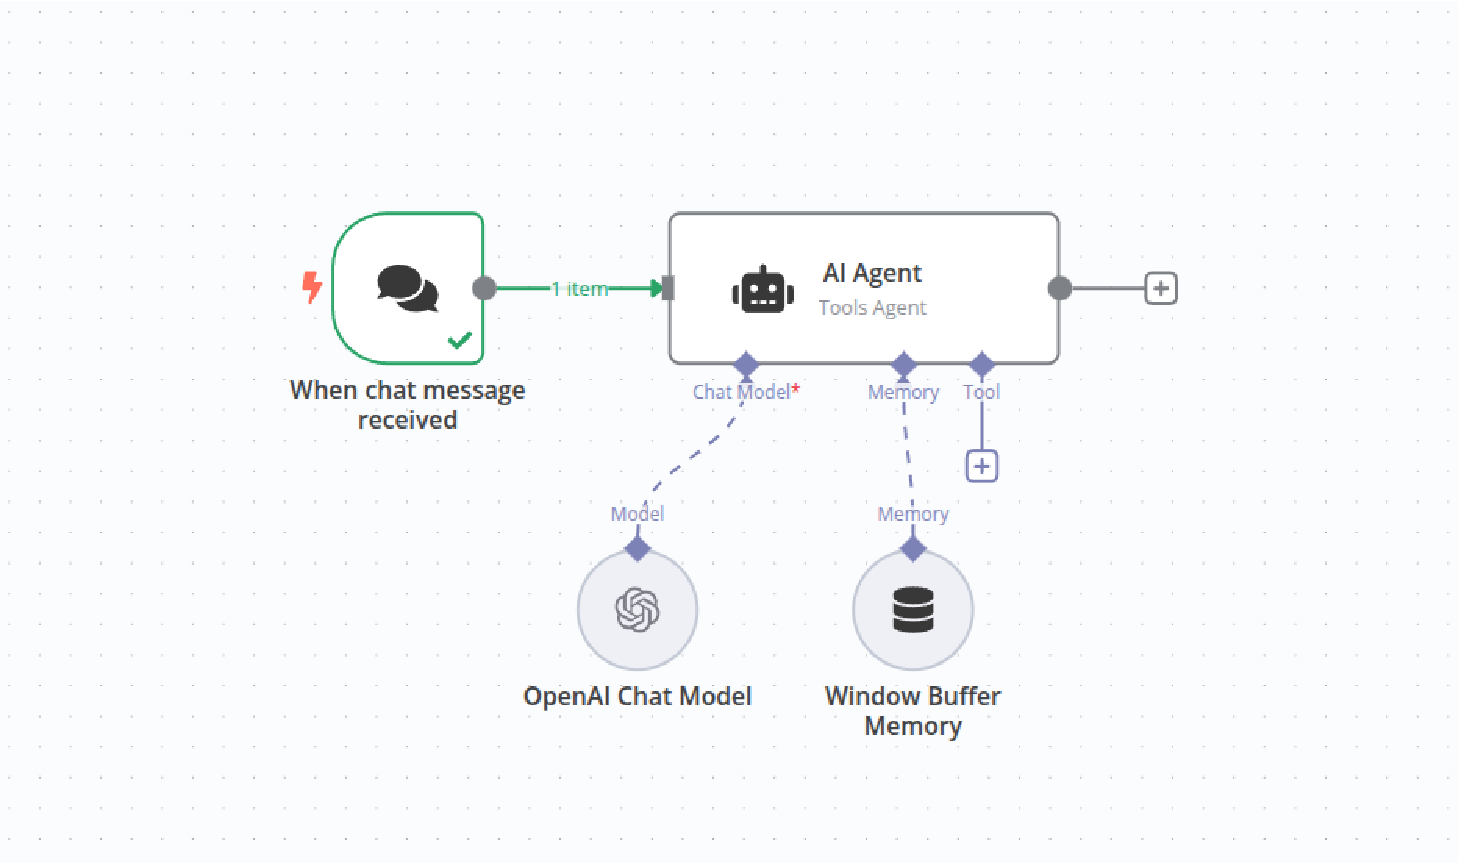
\includegraphics[width=1\linewidth]{Chap1-7/ai-intro01.pdf}
\end{figure}

AI Agent trong n8n là một node linh hoạt, đóng vai trò như một “trợ lý thông minh” trong các quy trình tự động hóa của bạn. Hãy tưởng tượng nó như một người bạn đồng hành có khả năng xử lý các tác vụ phức tạp mà không cần bạn phải viết mã từ đầu. AI Agent có thể được sử dụng để thực hiện nhiều nhiệm vụ khác nhau, từ trả lời câu hỏi, tạo nội dung, đến phân tích dữ liệu – tất cả đều dựa trên các mô hình ngôn ngữ lớn (LLM) mà bạn kết nối với nó.

Ví dụ, bạn có thể thiết lập một workflow để AI Agent tự động trả lời email khách hàng dựa trên nội dung họ gửi, hoặc phân loại các yêu cầu hỗ trợ trước khi chuyển đến đúng bộ phận. Để bắt đầu, bạn chỉ cần kết nối node này với một dịch vụ AI (như OpenAI) và định nghĩa nhiệm vụ cụ thể mà bạn muốn nó thực hiện. Đừng lo nếu bạn chưa quen – chúng ta sẽ đi qua từng bước thiết lập trong các ví dụ thực tế ở phần sau!


Đây là trung tâm điều phối dành cho các ứng dụng AI tự động. Nó có khả năng tiếp nhận yêu cầu, đưa ra quyết định và sử dụng các công cụ (tools) để thực hiện hành động nhằm đạt được mục tiêu cụ thể. n8n hỗ trợ nhiều loại agent khác nhau, bao gồm Conversational Agent (phục vụ hội thoại cơ bản), Tools Agent (có khả năng sử dụng công cụ), và SQL Agent (tương tác với cơ sở dữ liệu SQL).


Node này có thể kết nối với nhiều mô hình hội thoại AI thông qua các sub-node như OpenAI, Anthropic, Azure OpenAI, Ollama, Google Gemini/Vertex, Mistral, Groq và nhiều mô hình khác. Các công cụ mà agent có thể sử dụng cũng được tích hợp dưới dạng sub-node, ví dụ: Calculator, Code, HTTP Request, Vector Store Q\&A, Wikipedia, và đặc biệt là Custom n8n Workflow Tool (cho phép sử dụng một workflow khác như một công cụ riêng biệt).

Một thành phần quan trọng khác là các Output Parsers – những sub-node như Structured Output Parser, Item List Output Parser, và Auto-fixing Output Parser – giúp định dạng kết quả đầu ra và đảm bảo tính nhất quán trong phản hồi từ AI.

\subsubsection{Node Conversational AI Agent – Trò chuyện như con người}
Node Conversational Agent cho phép bạn xây dựng các cuộc trò chuyện tự nhiên giống như giữa con người với nhau. Nó có khả năng ghi nhớ ngữ cảnh, hiểu ý định của người dùng, và trả lời chính xác, phù hợp với nội dung cuộc hội thoại. Nếu có ý định làm một con chatbot, hệ thống hỗ trợ khách hàng, tư vấn đủ thứ thì dùng cái này là hợp lý.


Agent này mô tả các công cụ có thể dùng thông qua hệ thống prompt và xử lý các phản hồi JSON để gọi công cụ. Nếu bạn sử dụng một mô hình AI không hỗ trợ gọi công cụ, hoặc bạn chỉ cần xử lý hội thoại đơn giản, thì đây là một giải pháp đa năng – linh hoạt hơn so với Tools Agent, dù có thể kém chính xác hơn trong những tình huống chuyên biệt.

Để test được node này, quý vị có thể kết hợp với node "Chat Trigger" và chat trực tiếp trên giao diện canvas của n8n. Đồng thời để chatbot có thể nhớ được ngữ cảnh thì ta cần lưu ngữ cảnh vào một nơi gọi là bộ nhớ tạm thời "Memory sub-node" để duy trì cuộc trò chuyện trong xuyên suốt lúc nhắn, lưu ý là bộ nhớ không duy trì xuyên suốt giữa các phiên. Ví dụ đối với chăm sóc khách hàng trên facebook thì mỗi UserID sẽ có một sessionID tương ứng. 

\newpage

Cấu hình node Conversational Agent

\begin{figure}[htbp]
    \centering
    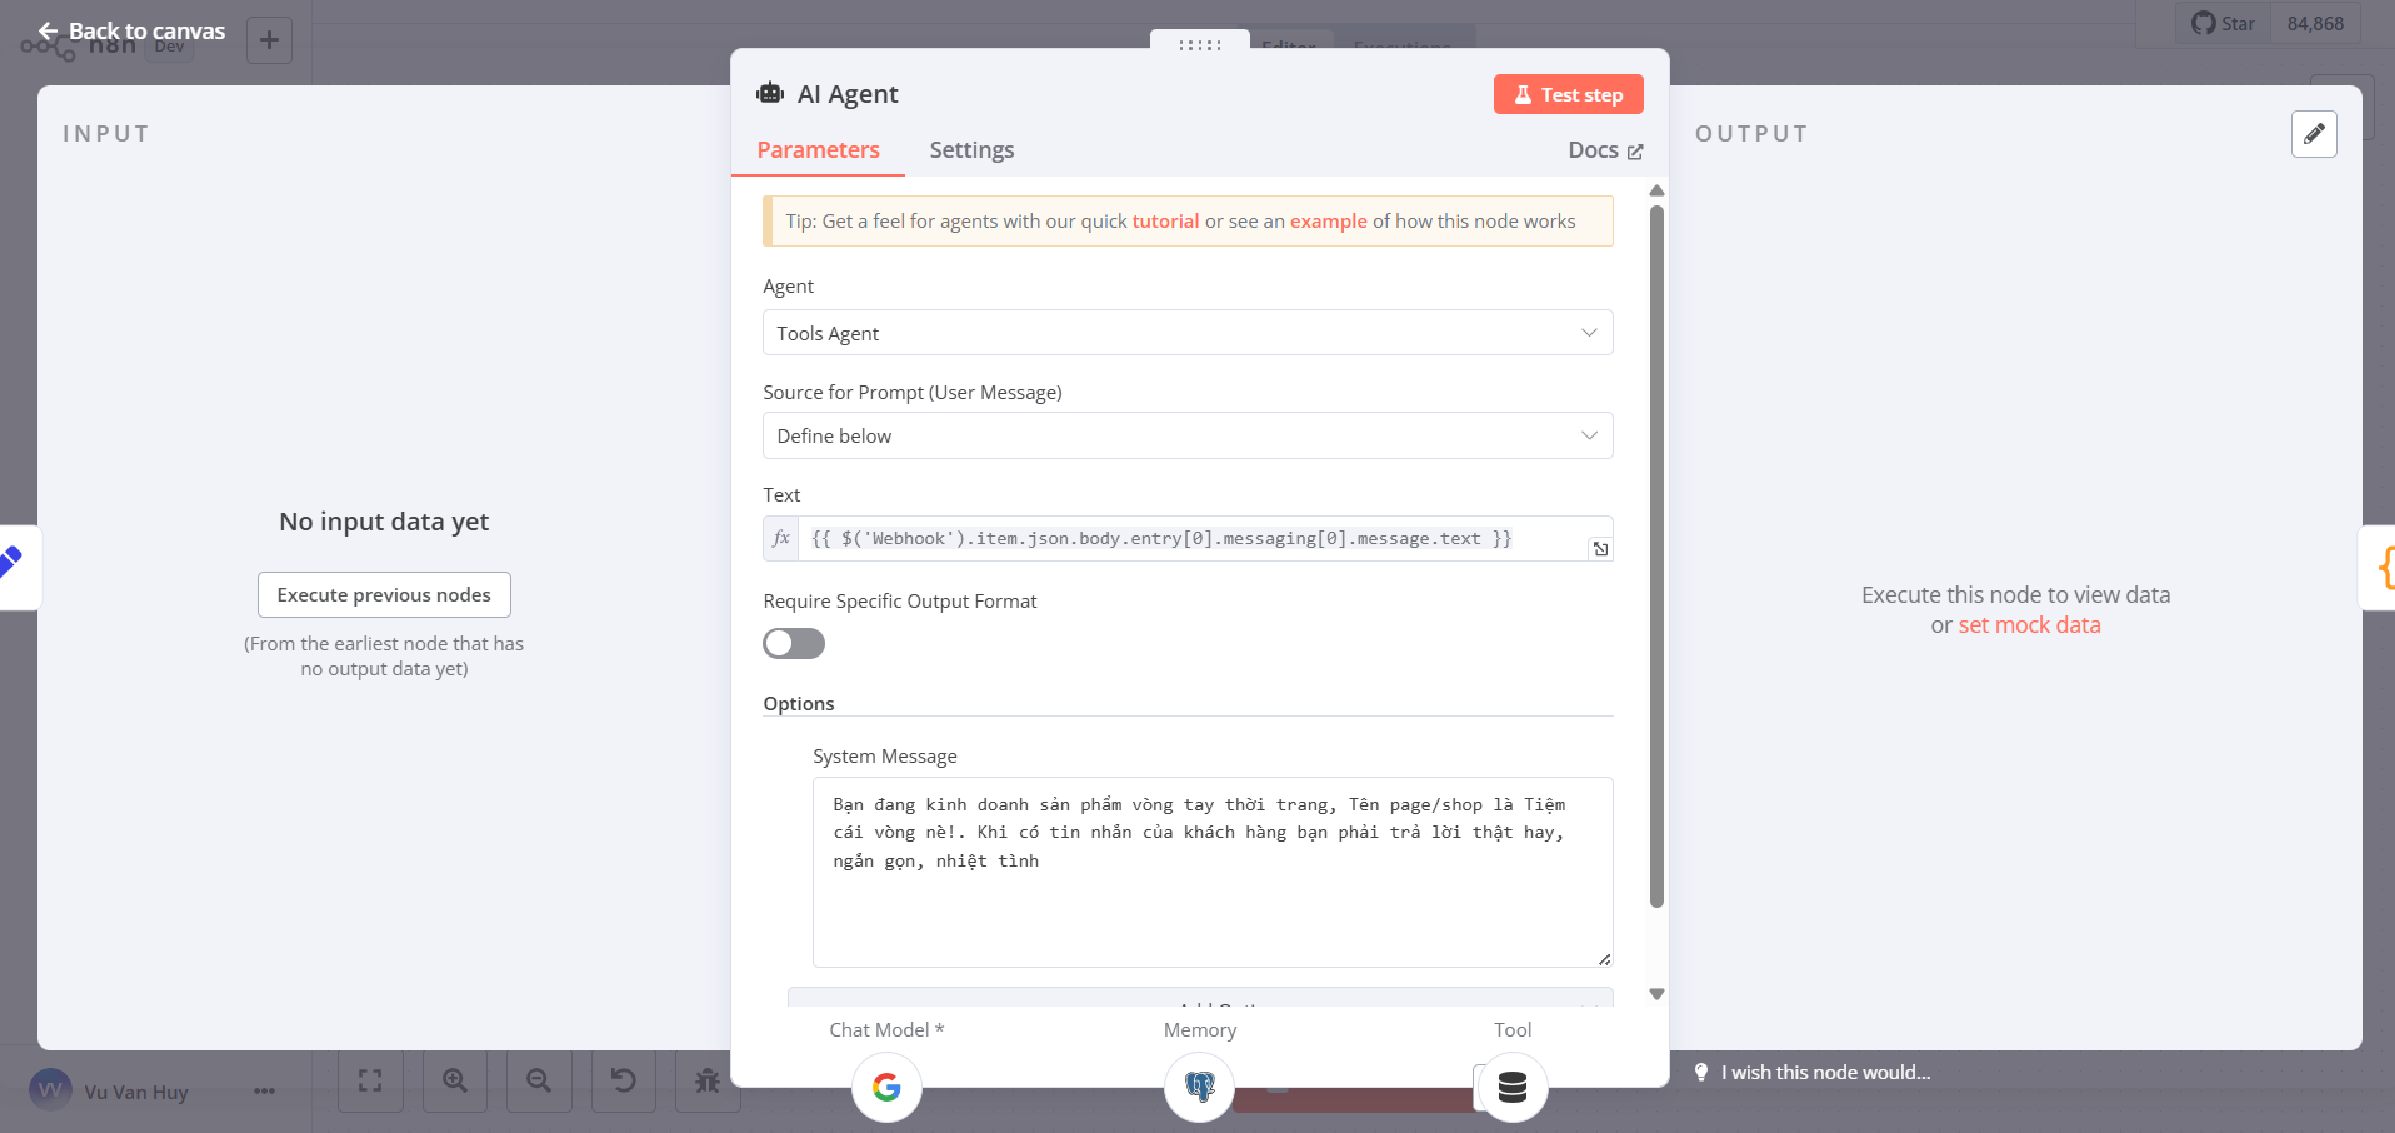
\includegraphics[width=1\linewidth]{Chap1-7/Agent-a.pdf}
\end{figure}

\begin{enumerate}
    \item Prompt – Tạo nội dung câu hỏi: 
    
    \begin{itemize}
        \item Chọn cách node nhận nội dung đầu vào (prompt) từ người dùng
        \item Tự động lấy từ node trước đó: Node sẽ lấy nội dung từ node có tên chatInput.
        \item Tự định nghĩa bên dưới: Bạn nhập văn bản tĩnh hoặc dùng biểu thức để tạo nội dung động trong phần "Prompt (User Message)".
    \end{itemize}

    \item Yêu cầu định dạng đầu ra cụ thể: Bạn có thể yêu cầu phản hồi từ AI theo định dạng nhất định chỉ bằng cách sửa prompt và yêu cầu nó. Khi bật tùy chọn này, n8n sẽ yêu cầu kết nối với một trong các node phân tích đầu ra sau:
    \begin{itemize}
        \item Auto-fixing Output Parser

        \item Item List Output Parser

        \item Structured Output Parser
    \end{itemize}

    \item Tùy chọn nâng cao cho Conversational Agent: Cho Agent biết về các công cụ  mà nó có thể thêm vào ngữ cảnh thông tin đầu vào của người dùng. Ví dụ thêm cho nó 1 cái database để select data.

\textbf{Human Message}

Đây là phần bạn mô tả:
\begin{itemize}
    \item Công cụ mà AI có thể sử dụng ({tools})

    \item Cách định dạng đầu ra ({format\_instructions})

    \item Câu hỏi hoặc yêu cầu từ người dùng ({{input}})

\end{itemize}
Một ví dụ cấu trúc thông điệp:
\begin{verbatim}
TOOLS
------
Assistant có thể yêu cầu người dùng sử dụng các công cụ sau để tìm thông tin hỗ trợ cho câu hỏi:

{tools}

{format_instructions}

USER'S INPUT
--------------------
Đây là yêu cầu của người dùng (hãy trả lời bằng đoạn mã JSON chứa một hành động duy nhất, KHÔNG thêm nội dung khác):

{{input}}
\end{verbatim}

\textbf{System Message}

Hiểu như này cho dễ hiểu. System prompt kiểu như đặt ngữ cảnh cho con chatbot hiểu. Mem có thể nhập vào đó là hãy trả lời như một ông cụ 60 tuổi chẳng hạn. Agent nó sẽ đặt mình vào bối cảnh đó và phản hồi lại cho phù hợp. Điều này làm cho con bot hiểu rõ vai trò, giọng điệu, hoặc cách phản hồi như nào sao cho đúng ý.

Ví dụ: Hãy nói chuyện như một ông cụ 60 tuổi đang khù khụ với với người bạn hiền về cuộc sống, hãy bắt đầu

Respone: À… khụ khụ… chà… lâu lắm rồi mới có người ngồi đây hàn huyên với lão già này đấy. Ờ… cái tuổi sáu mươi rồi, sáng dậy thì lưng còng, tối đến thì đầu gối kêu răng rắc… mà vẫn ham ngồi kể chuyện xưa chuyện nay. Khụ khụ…

Này… anh bạn hiền, cậu ngồi xuống đây, rót chén trà nóng đi. Thời buổi bây giờ nhanh quá… mới hôm nào còn bẻ đôi cái bánh đa, ngồi ven sông thả câu, thế mà quay đi quay lại tóc tôi đã bạc trắng thế này rồi. Anh bạn thì sao? Dạo này cuộc sống ra sao? Ừm… có cái gì vui kể lão nghe với.

$\rightarrow$ Hãy ghê :>
    \item Max Iterations: Số lần mô hình có thể chạy lặp lại để tạo ra phản hồi tốt nhất. Mặc định là 10 lần.

    \item Trả về các bước trung gian: Bạn có thể chọn bật hoặc tắt việc trả lại các bước xử lý trung gian mà agent đã thực hiện. Đây là cách hữu ích để gỡ lỗi hoặc hiểu rõ logic xử lý của mô hình AI.
\end{enumerate}


Tôi chỉ giới thiệu các option này thôi, mọi người có thể vào để nghịch nghịch thử là biết ngay à. Easy thuiii!


\subsection{OpenAI}
Node OpenAI trong n8n là cầu nối giúp bạn dễ dàng tích hợp sức mạnh của các mô hình AI hàng đầu như GPT-4, GPT-3.5, DALL·E và nhiều mô hình khác vào quy trình tự động hóa của mình. Với node này, bạn có thể thực hiện hàng loạt tác vụ thông minh như tạo văn bản, phân tích cảm xúc, tóm tắt nội dung, sinh hình ảnh và nhiều hơn thế — tất cả đều được thực hiện tự động ngay trong workflow của bạn.

OpenAI hiện là một trong những nền tảng AI phổ biến và được ứng dụng rộng rãi nhất mà n8n hỗ trợ. Nhờ node này, khả năng xử lý ngôn ngữ tự nhiên (NLP) tiên tiến của các mô hình như GPT-3 hay GPT-4 nằm gọn trong tay bạn: từ việc sinh nội dung, trả lời câu hỏi, dịch thuật, viết mã lập trình đến xây dựng chatbot hoặc trợ lý ảo.

\textbf{Bạn có thể làm được gì với OpenAI Node?}

Hãy thử tưởng tượng bạn chỉ cần nhập vài từ khóa, OpenAI sẽ tự động viết bài blog hoàn chỉnh cho bạn. Hay khi có khách hàng gửi email hỏi thông tin sản phẩm, hệ thống có thể lập tức sinh câu trả lời thông minh mà không cần ai can thiệp. Hoặc, bạn muốn tạo hình ảnh minh họa cho bài viết? Chỉ cần một prompt mô tả, DALL·E sẽ xử lý ngay.

\textbf{Cách sử dụng rất đơn giản:}

Bạn chỉ cần có API Key từ OpenAI, kết nối vào node và định nghĩa prompt — chính là câu lệnh, câu hỏi hoặc yêu cầu mà bạn muốn AI thực hiện. Ví dụ, prompt: “Hãy viết một đoạn giới thiệu ngắn về n8n bằng tiếng Việt” sẽ cho bạn kết quả trong vài giây.

Trong chương này, bạn sẽ được hướng dẫn thiết lập một workflow thực tế sử dụng OpenAI Node, để trực tiếp trải nghiệm khả năng tự động hóa kết hợp AI mạnh mẽ ngay trong n8n.



\newpage
\subsection{Basic LLM Chain}
\begin{figure}[htbp]
    \centering
    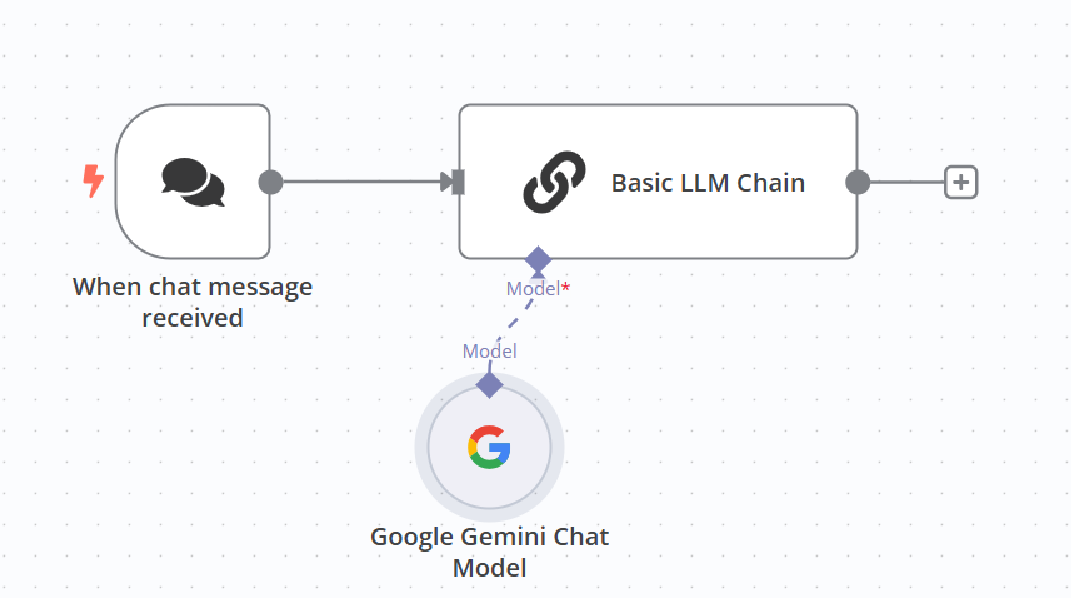
\includegraphics[width=1\linewidth]{Chap1-7/basic_llm.pdf}
\end{figure}
Basic LLM Chain là một node cơ bản nhưng cực kỳ hữu ích để làm việc với các mô hình ngôn ngữ lớn (LLM). Đây là điểm khởi đầu lý tưởng nếu bạn mới bắt đầu khám phá AI trong n8n. Node này cho phép bạn gửi một đoạn văn bản hoặc câu hỏi đến LLM và nhận lại phản hồi – đơn giản nhưng đầy tiềm năng.

Ví dụ, bạn có thể dùng Basic LLM Chain để tạo tiêu đề email tự động dựa trên nội dung, hoặc chuyển đổi một đoạn văn bản dài thành câu hỏi ngắn gọn. Cách hoạt động rất dễ hiểu: bạn cung cấp đầu vào (input), chọn mô hình LLM (như OpenAI hoặc các dịch vụ khác được hỗ trợ), và nhận đầu ra (output). Điều tuyệt vời là bạn không cần phải là chuyên gia AI để sử dụng – chỉ cần một chút sáng tạo và ý tưởng về những gì bạn muốn đạt được. Chúng ta sẽ thử một dự án nhỏ với node này để bạn làm quen ngay trong phần thực hành.
\subsection{Information Extractor}

\begin{figure}[htbp]
    \centering
    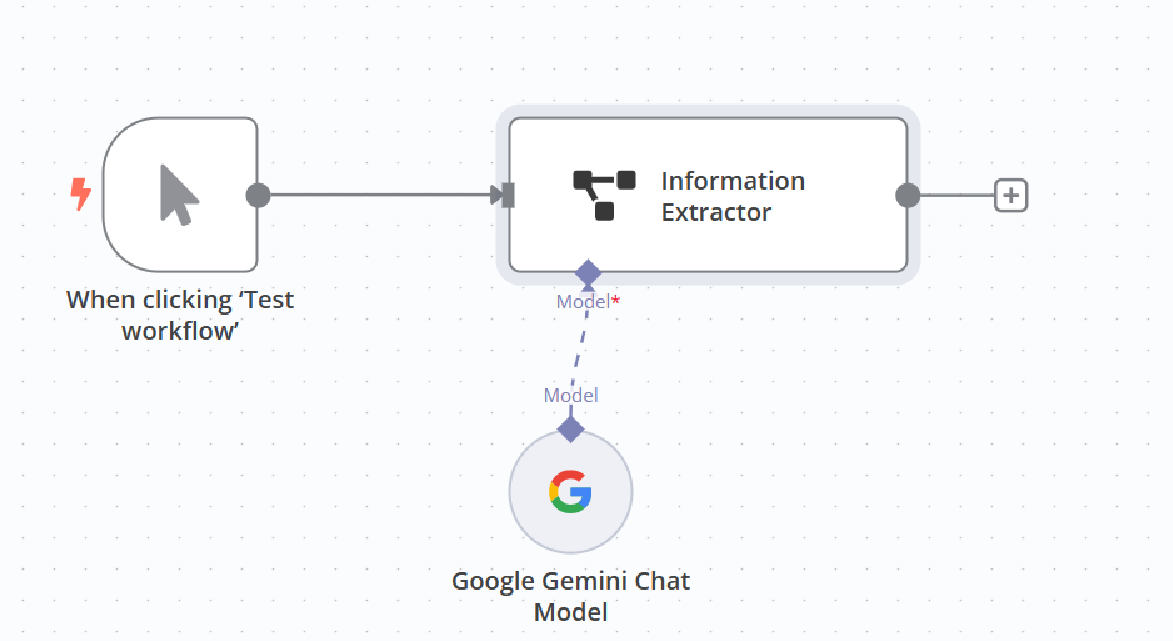
\includegraphics[width=1\linewidth]{Chap1-7/info_extract.pdf}
\end{figure}

Information Extractor là nút AI trong n8n giúp trích xuất thông tin cụ thể từ văn bản đầu vào. Nút này đặc biệt hữu ích khi bạn cần phân tích và lấy dữ liệu có cấu trúc từ nội dung phi cấu trúc như email, báo cáo, mô tả sản phẩm, bài đăng trên mạng xã hội hoặc văn bản tự do khác.

Nút này sử dụng sức mạnh của các mô hình AI để hiểu ngữ cảnh và tự động trích xuất thông tin theo cấu trúc bạn chỉ định, giúp tiết kiệm thời gian và giảm thiểu lỗi so với việc xử lý thủ công.


\textbf{Schema}

Lược đồ xác định cấu trúc của thông tin bạn muốn trích xuất. Bạn cần chỉ định một đối tượng JSON với các trường và kiểu dữ liệu tương ứng:

\begin{itemize}
    \item string: Trích xuất văn bản
    \item number: Trích xuất giá trị số
    \item boolean: Trích xuất giá trị đúng/sai
    \item array: Trích xuất danh sách các giá trị
    \item object: Trích xuất đối tượng lồng nhau với cấu trúc riêng
\end{itemize}

Hiểu đơn giản như bỏ một đoạn hồ sơ ứng viên vào sau đó nhập prompt bảo con GPT là nhặt ra cho tôi các thông tin này thông tin kia và trả về định dạng json. 

Cái này được ứng dụng nhiều trong trích xuất thông tin từ tin nhắn của khách hàng, hay email phản hồi, tự động nhập dữ liệu 



\newpage
\subsection{Question and Answer Chain}
\begin{figure}[htbp]
    \centering
    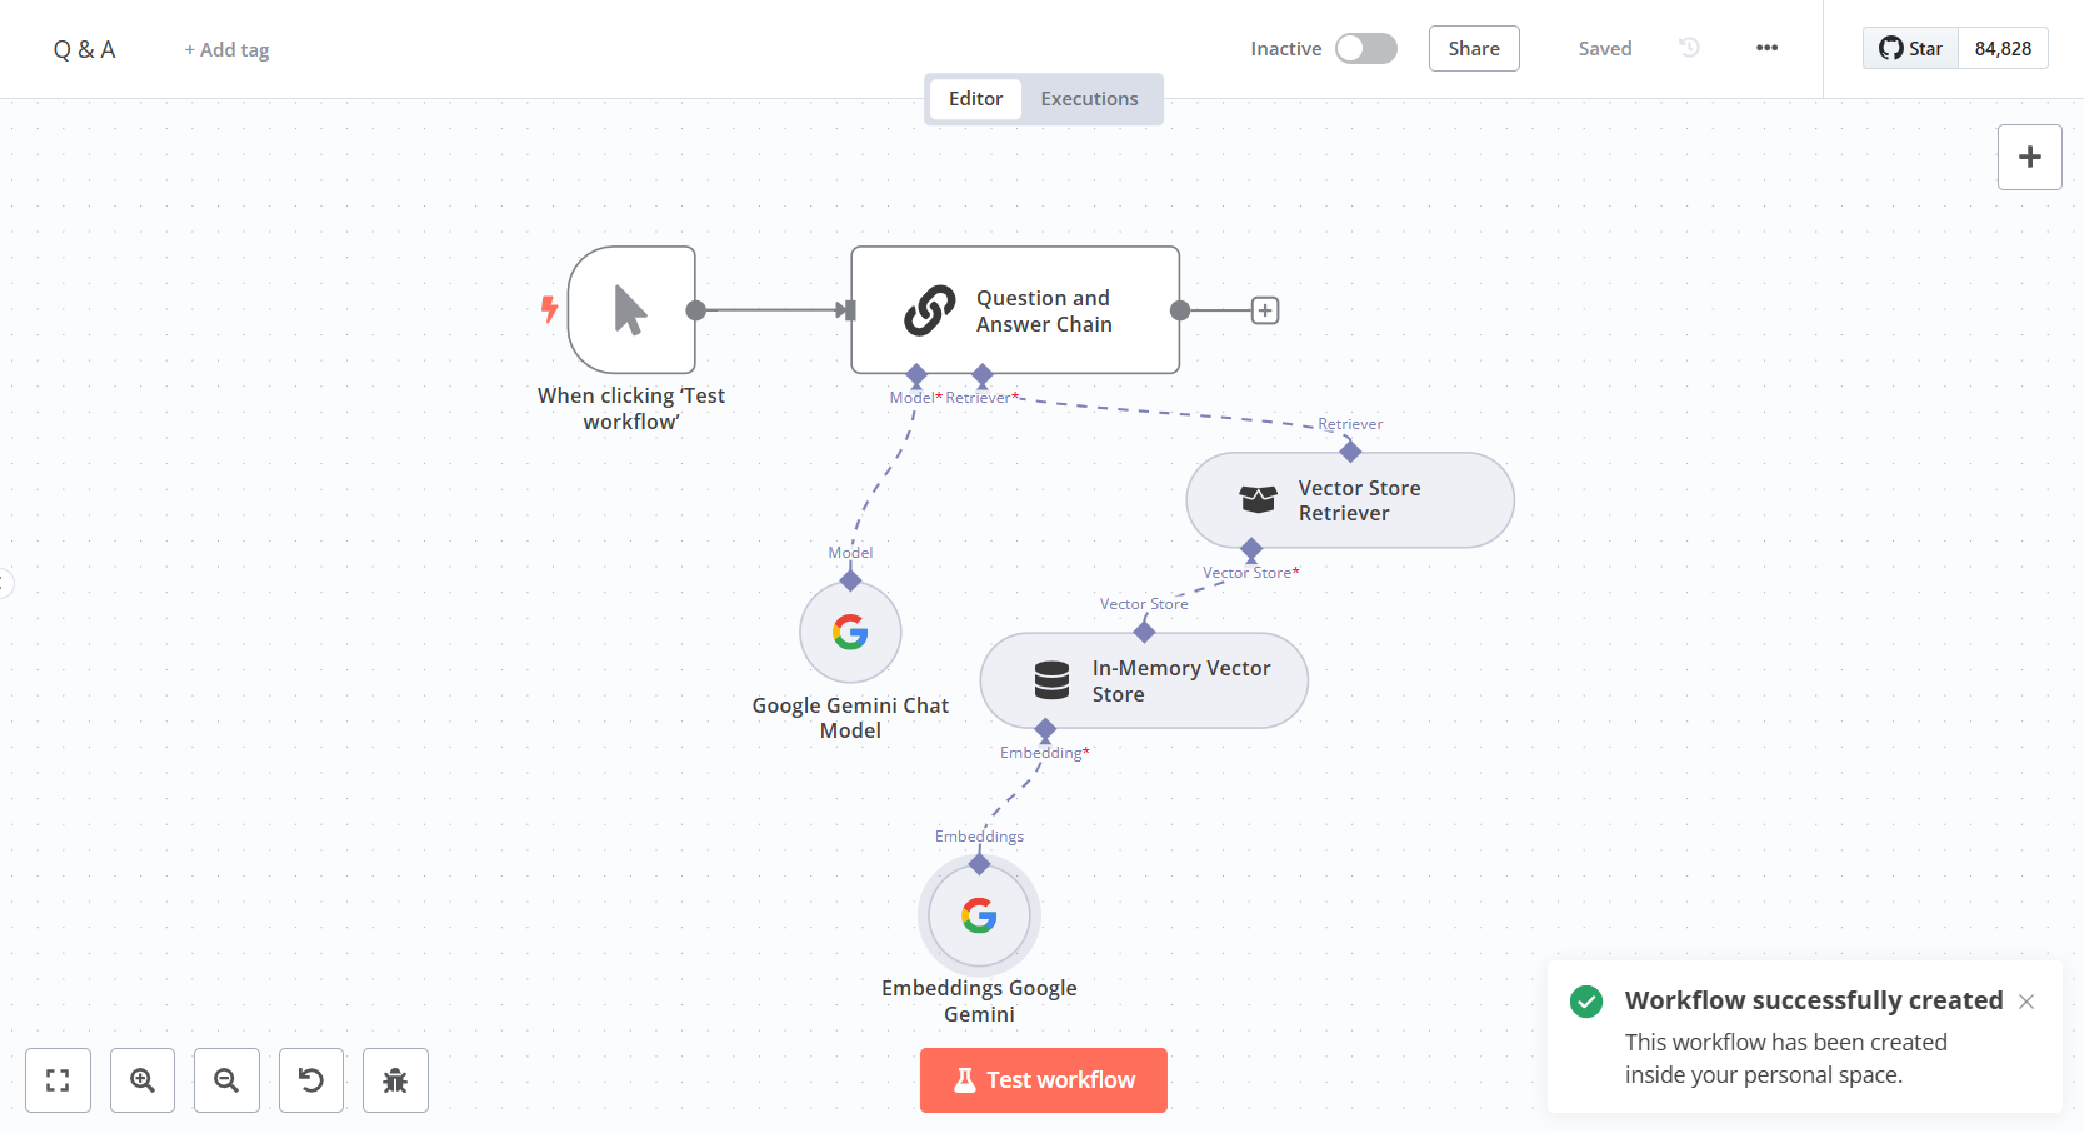
\includegraphics[width=1\linewidth]{Chap1-7/Q & A.pdf}
\end{figure}

Node này liên quan đến các bài toán liên quan đến RAG - hơi kĩ thuật hơn chút

Question and Answer Chain (Chuỗi Hỏi Đáp) là một nút AI mạnh mẽ trong n8n giúp tạo ra hệ thống trả lời câu hỏi thông minh dựa trên nguồn dữ liệu của riêng bạn. Nút này kết hợp khả năng của các mô hình ngôn ngữ lớn (LLM) với dữ liệu của bạn để tạo ra một hệ thống có thể trả lời các câu hỏi cụ thể với thông tin chính xác và phù hợp.

Điểm mạnh của Question and Answer Chain là khả năng tìm kiếm và trích xuất thông tin từ nguồn dữ liệu của bạn, sau đó sử dụng AI để tạo ra câu trả lời trôi chảy, tự nhiên dựa trên dữ liệu đó. Điều này đặc biệt hữu ích khi bạn muốn tạo ra một chatbot hoặc hệ thống trợ lý ảo có thể trả lời câu hỏi từ tài liệu nội bộ, cơ sở kiến thức hoặc nguồn dữ liệu khác.

\textbf{Cách nó hoạt động}

Question and Answer Chain hoạt động theo các bước cơ bản sau:
\begin{itemize}
    \item Nhận câu hỏi từ người dùng
    \item Tìm kiếm và truy xuất thông tin liên quan từ nguồn dữ liệu đã được cung cấp
    \item Phân tích thông tin để hiểu nội dung và ngữ cảnh
    \item Tạo câu trả lời dựa trên thông tin đã thu thập, sử dụng mô hình ngôn ngữ
    \item Trả về kết quả cho người dùng một cách tự nhiên và dễ hiểu
\end{itemize}

$\Rightarrow$ Đầu ra thường là các trợ lý ảo, chatbot thông minh.   


\subsection{Sentiment Analysis}

\begin{figure}[htbp]
    \centering
    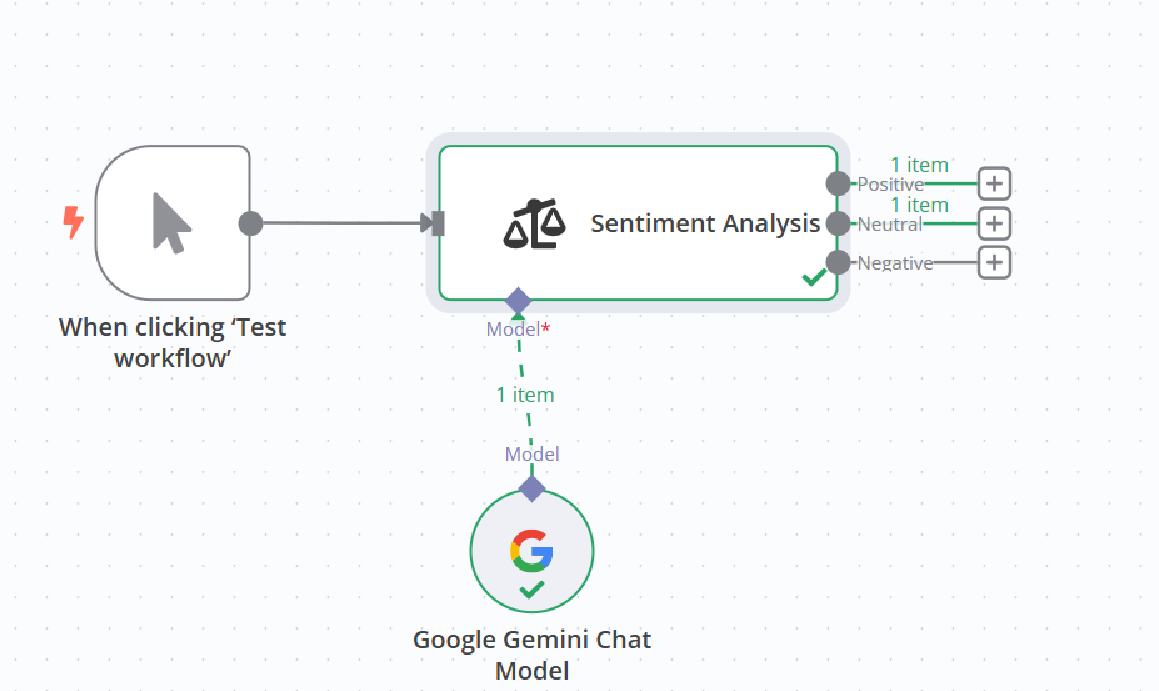
\includegraphics[width=1\linewidth]{Chap1-7/sentiment-node.pdf}
\end{figure}

Phân tích cảm xúc (Sentiment Analysis hay Opinion Mining) là một trong những ứng dụng giá trị và thiết thực nhất của AI trong lĩnh vực xử lý ngôn ngữ tự nhiên (NLP). Công nghệ này cho phép máy tính “đọc hiểu” thái độ, cảm xúc và quan điểm ẩn chứa trong văn bản — liệu chúng là tích cực, tiêu cực hay trung tính. Trong bối cảnh dữ liệu văn bản được tạo ra liên tục trên mạng xã hội, đánh giá sản phẩm, email, khảo sát… khả năng tự động phân tích cảm xúc giúp tổ chức nắm bắt phản hồi nhanh chóng, theo dõi hình ảnh thương hiệu và ra quyết định dựa trên dữ liệu thực tế.

Với n8n, bạn có thể dễ dàng xây dựng các quy trình tự động hóa để thu thập văn bản từ nhiều nguồn khác nhau, chuyển đến mô hình AI xử lý cảm xúc và thực hiện các hành động tương ứng dựa trên kết quả phân tích.

Thông thường, Sentiment Analysis sẽ phân loại văn bản vào ba nhóm chính:
\begin{itemize}
    \item Tích cực (Positive): Thể hiện sự hài lòng, khen ngợi hoặc ủng hộ.

    \item Tiêu cực (Negative): Thể hiện sự không hài lòng, phàn nàn hoặc chỉ trích.

    \item Trung tính (Neutral): Các câu thông báo, sự kiện khách quan, không chứa cảm xúc rõ ràng.
\end{itemize}


Các trường hợp ứng dụng phổ biến:
\begin{itemize}
    \item Giám sát Thương hiệu (Brand Monitoring): Tự động thu thập và phân loại cảm xúc từ các lượt đề cập thương hiệu trên mạng xã hội, diễn đàn, và báo chí — giúp doanh nghiệp kịp thời nắm bắt hình ảnh công chúng.

    \item Phân tích Phản hồi Khách hàng:
\begin{itemize}
    \item Tự động phân loại các đánh giá sản phẩm, bình luận trên trang thương mại điện tử.
    \item Đánh giá cảm xúc trong email hỗ trợ khách hàng hoặc các phiếu khảo sát mức độ hài lòng (CSAT/NPS).
\end{itemize}

    \item Quản lý Trải nghiệm Khách hàng: Xác định nhanh các khách hàng có cảm xúc tiêu cực để ưu tiên hỗ trợ, chăm sóc hoặc xử lý sự cố.

    \item Nghiên cứu Thị trường: Phân tích cảm xúc cộng đồng đối với sản phẩm mới, chiến dịch quảng cáo hoặc các xu hướng xã hội.

    \item Phân loại Nội dung: Tự động gắn nhãn cảm xúc cho bài viết, bình luận trên diễn đàn, mạng xã hội hay website.

\end{itemize}


\subsection{Summarization Chain}
Trong kỷ nguyên bùng nổ thông tin như hiện nay, nhu cầu tóm tắt văn bản ngày càng trở nên thiết yếu. Từ email, báo cáo, bài báo cho đến bản ghi cuộc họp, việc nhanh chóng nắm bắt nội dung chính giúp tiết kiệm thời gian và nâng cao hiệu quả làm việc.

Sự phát triển vượt bậc của Trí tuệ nhân tạo, đặc biệt là các Mô hình Ngôn ngữ Lớn (LLMs), đã mở ra khả năng tóm tắt văn bản một cách tự nhiên và chính xác. Không chỉ dừng lại ở việc phân tích dữ liệu thô, AI giờ đây có thể tạo ra những bản tóm tắt súc tích, đúng trọng tâm và phù hợp với ngữ cảnh sử dụng.

Trong bối cảnh đó, n8n nổi lên như một nền tảng tự động hóa linh hoạt, cho phép người dùng xây dựng các quy trình xử lý dữ liệu kết hợp với sức mạnh của AI. Đặc biệt, với tính năng thiết lập các chuỗi workflow (chains), n8n giúp kết nối nhiều bước xử lý khác nhau — từ tiếp nhận văn bản, truyền dữ liệu đến AI, lấy kết quả tóm tắt và gửi đi hoặc lưu trữ. Summarization Chain chính là một workflow như vậy, được thiết kế chuyên biệt để tự động hóa việc tóm tắt nội dung.

Các trường hợp ứng dụng phổ biến:

\begin{itemize}
    \item Tóm tắt Email/Chuỗi Email: Tự động trích xuất và tổng hợp ý chính từ các email quan trọng hoặc các cuộc trao đổi dài dòng.

    \item Tóm tắt Báo cáo/Tài liệu: Rút gọn nội dung của báo cáo doanh nghiệp, tài liệu kỹ thuật hoặc nghiên cứu chuyên sâu, giúp người đọc nắm được thông tin trọng yếu nhanh chóng.

    \item Tóm tắt Bản ghi Cuộc họp: Chuyển bản ghi họp thành danh sách các quyết định và nhiệm vụ hành động ngắn gọn, dễ theo dõi.

    \item Tóm tắt Tin tức/Bài báo: Tạo feed tin tức cá nhân hóa với bản tóm tắt ngắn gọn từ nhiều nguồn báo chí khác nhau.

    \item Phân tích Phản hồi Khách hàng: Tổng hợp những ý kiến nổi bật từ hàng trăm đánh giá, khảo sát hoặc bình luận mạng xã hội.

    \item Tạo Mô tả ngắn (Abstracts): Tự động sinh bản tóm tắt cho bài viết blog, báo cáo khoa học hoặc nội dung truyền thông.
\end{itemize}

Lựa chọn Mô hình AI và Tinh chỉnh (Choosing Models \& Fine-tuning):
\begin{itemize}
    \item GPT-4/Claude 3 Opus: Chất lượng cao nhất, hiểu ngữ cảnh tốt, nhưng đắt hơn và chậm hơn.
    \item GPT-3.5 Turbo/Claude 3 Sonnet/Gemini Pro: Cân bằng tốt giữa chi phí, tốc độ và chất lượng. Thường là lựa chọn tốt để bắt đầu.
    \item Hugging Face/Ollama: Linh hoạt, có thể chọn mô hình chuyên biệt cho tóm tắt, có thể chạy cục bộ (Ollama) để tiết kiệm chi phí hoặc bảo mật dữ liệu, nhưng đòi hỏi cấu hình phức tạp hơn.
    \item Prompt Engineering: Nhấn mạnh tầm quan trọng của việc viết prompt rõ ràng, chi tiết. Thử nghiệm với các kiểu prompt khác nhau để đạt kết quả tốt nhất (ví dụ: yêu cầu độ dài cụ thể, giọng văn, đối tượng người đọc, các điểm cần tập trung).
    \item Tham số Model: Giới thiệu sơ qua về các tham số như temperature (ảnh hưởng độ sáng tạo/ngẫu nhiên), max\_tokens (giới hạn độ dài output).
\end{itemize}


\section{Khi Tự Động Hóa Gặp Trí Tuệ Nhân Tạo}
Tôi vẫn nhớ dự án đầu tiên suýt "đổ bể" khi cố gắng tích hợp AI vào quy trình kinh doanh. Hồi đó, tôi nghĩ việc kết nối các dịch vụ AI sẽ đơn giản như việc nối các đoạn ống nước. Thực tế hoàn toàn khác.


\subsection{Dự Án Điển Hình 1: Hệ Thống Quản Lý Khiếu Nại Thông Minh}
\textbf{Bối Cảnh Thực Tế:}

Một công ty logistics tiếp nhận hơn 500 khiếu nại mỗi tháng qua email, điện thoại và mạng xã hội. Nhân viên phải xử lý thủ công bằng giấy tờ và file Excel, gây quá tải và dễ sai sót. Hệ thống cũ không thể theo dõi, tổng hợp hay cảnh báo kịp thời, ảnh hưởng đến trải nghiệm khách hàng và uy tín công ty.

Giải pháp bằng AI: sử dụng n8n để tự động thu thập khiếu nại từ email, form và API mạng xã hội, lưu vào cơ sở dữ liệu tập trung. Kết hợp AI để phân loại nội dung khiếu nại theo mức độ ưu tiên và chủ đề. Hệ thống sẽ tự động gửi thông báo đến bộ phận liên quan và cập nhật trạng thái xử lý. Ngoài ra, n8n còn tạo báo cáo hàng ngày và gửi email thống kê cho quản lý mà không cần thao tác thủ công.



\subsection{Dự án Điển Hình 2: Trích xuất thông tin từ kho dữ liệu hồ sơ ứng viên}


% Bạn là một HR, hằng ngày bạn phải mày mò phát nhọc với hàng loạt CV của ứng viên. Đối với các ngân hàng lớn, big tech như viettel, cmc. Mỗi đợt tuyển dụng sẽ có lượng hồ sơ kinh khủng. Để sử lý lượng CV này đòi hỏi nhiều thời gian và công sức

Tuyển dụng là một quá trình tốn nhiều thời gian và nguồn lực, thường đầy rẫy thách thức. Từ việc tìm kiếm và sàng lọc ứng viên đến tiến hành phỏng vấn và đánh giá nhân tài, các nhà tuyển dụng cần phải điều hướng nhiều nhiệm vụ khác nhau để tìm ra ứng viên phù hợp với nhu cầu của công ty. Theo nghiên cứu của Glassdoor - Website tổng hợp đánh giá của nhân viên về doanh nghiệp họ đã và đang làm việc, trung bình doanh nghiệp mất 23 ngày để tìm kiếm ứng viên phù hợp và 1/3 thời gian trong tháng sử dụng để phỏng vấn ứng viên. Nhưng với sự phát triển của AI, nhiều nhiệm vụ trong số này hiện có thể được đơn giản hóa và tự động hóa, giúp các nhà quản lý tuyển dụng tiết kiệm thời gian và nguồn lực. Workflow này ra đời nhằm giải quyết vấn đề này, hỗ trợ người HR giảm thiểu thời gian tìm kiếm ứng viên phù hợp thông qua việc tương tác với chatbot, được huấn luyện bởi các mô hình ngôn ngữ lớn, và áp dụng các kỹ thuật tối ưu cho bài toán tìm kiếm thông tin.













Bằng cách sử dụng giải pháp này, các nhà tuyển dụng có thể tiết kiệm thời gian và công sức, cải thiện chất lượng ứng viên phù hợp, giảm thiên vị và đưa ra quyết định dựa trên dữ liệu. AI cho tuyển dụng có tiềm năng cách mạng hóa bối cảnh tuyển dụng bằng cách tăng hiệu quả, độ chính xác và hiệu quả chung trong việc xác định và thu hút nhân tài phù hợp cho các tổ chức. Trong khi các nhà tuyển dụng có thể dành vô số giờ để thẩm định nhân viên tiềm năng, phần mềm AI có thể xử lý lượng dữ liệu khổng lồ và chỉ trong vài giờ hoặc thậm chí vài phút, phân tích những ứng viên tiềm năng nào có thể phù hợp với công việc. Phần mềm AI có thể khớp trình độ và yêu cầu công việc với kỹ năng và kinh nghiệm của ứng viên, nhanh chóng phân loại sơ yếu lý lịch không phù hợp. Bộ phận nhân sự cũng có thể làm cho quy trình tuyển dụng hiệu quả hơn và tiết kiệm thời gian, cuối cùng giúp các nhà tuyển dụng tiết kiệm tiền. Đây là khía cạnh quan trọng cần cân nhắc khi nói đến tài chính của bất kỳ doanh nghiệp nào. Việc hợp lý hóa quy trình tuyển dụng, tuyển dụng và tuyển dụng sẽ giúp giảm chi phí, dẫn đến sự kết hợp thuận lợi giữa chi phí thấp hơn và năng suất tăng lên.

%%%%Chương 8
\chapter{Case Study thực tế (phần 1)}


%-------------------------------------------------------------
\section{\textbf{Dự án 1: Scrape google maps lấy dữ liệu khách hàng theo lĩnh vực yêu cầu }}

\href{https://drive.google.com/drive/folders/1IktM6xKkNLkmaOFLUl4w3Ezc7U0SJUlL?usp=sharing}{\textbf{\underline {Link tải workflow}}}

    \begin{figure}[H]
    \centering
    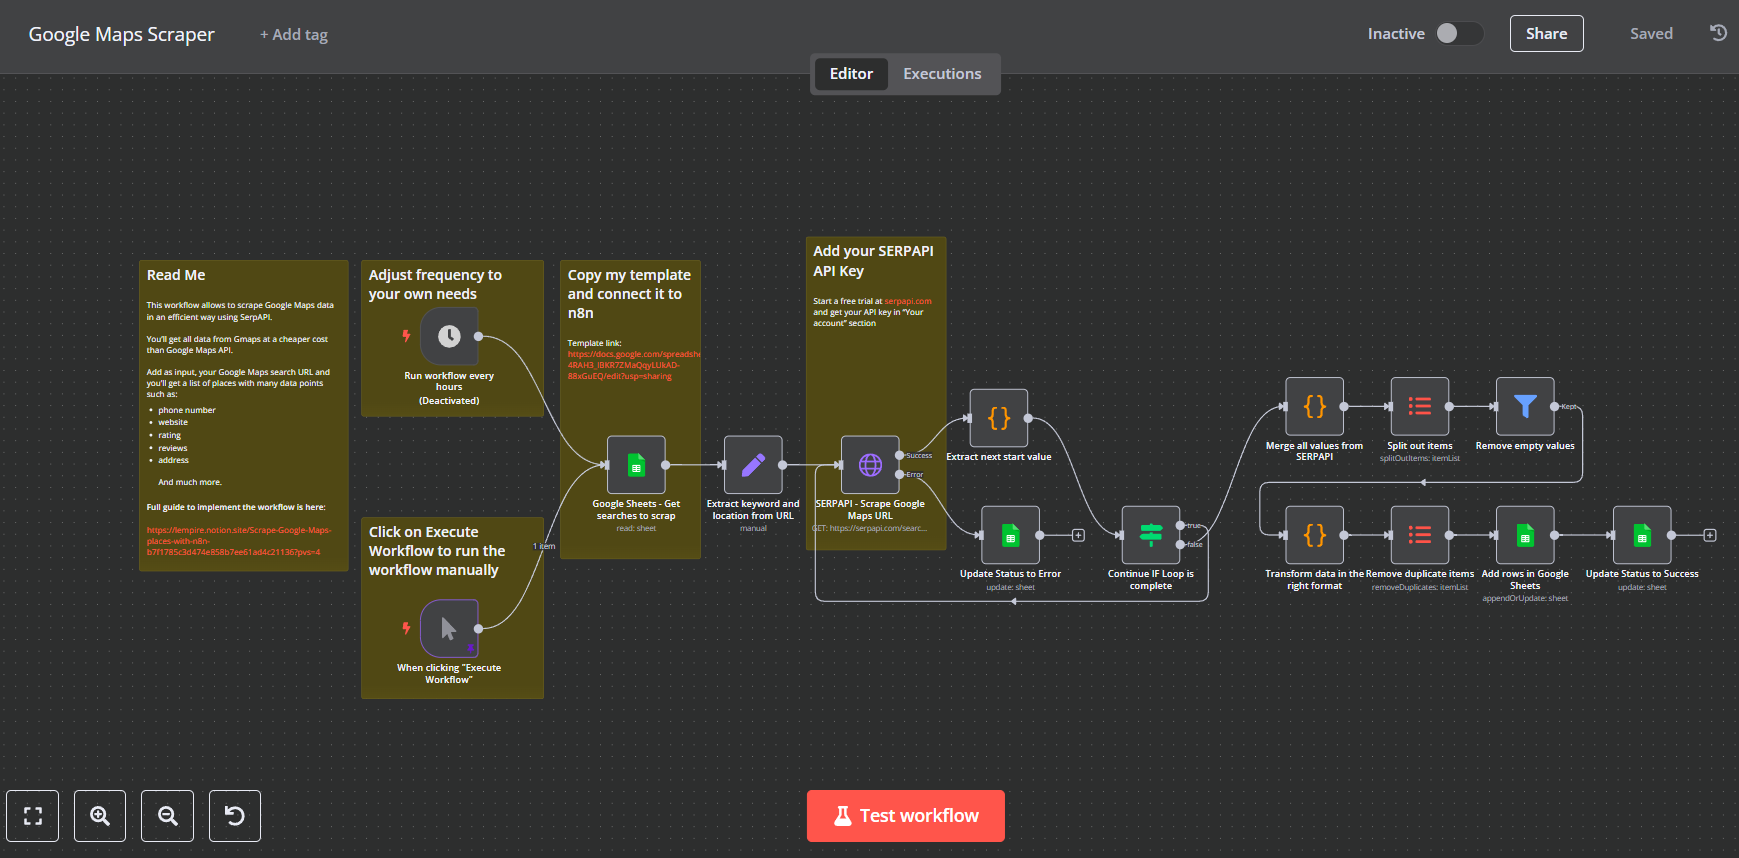
\includegraphics[width=1\textwidth]{images/2scrape01.png}
    \caption{Workflow Scrape google maps}
    \end{figure}

Đây là một workflow được thiết kế để tự động thu thập (scrape) dữ liệu từ Google Maps sử dụng SerpAPI. Workflow này được tạo trong n8n - một nền tảng tự động hóa quy trình làm việc (workflow automation platform).

\subsection{Tổng quan về Workflow}

Workflow này giúp bạn:
\begin{itemize}
  \item Thu thập thông tin về các địa điểm trên Google Maps (tên, số điện thoại, website, đánh giá, địa chỉ, v.v.)
  \item Lưu trữ dữ liệu vào Google Sheets
  \item Tự động lặp qua nhiều trang kết quả
  \item Theo dõi trạng thái của các yêu cầu scraping
\end{itemize}

\subsection{Các thành phần chính}

\begin{enumerate}
  \item \textbf{Trigger (Kích hoạt)}: Khởi chạy workflow bằng tay hoặc tự động theo lịch
  \item \textbf{API SerpAPI}: Sử dụng để truy vấn dữ liệu từ Google Maps
  \item \textbf{Google Sheets}: Lấy danh sách URL cần scrape và lưu kết quả
  \item \textbf{Code nodes}: Xử lý dữ liệu và quản lý việc phân trang
\end{enumerate}

\subsection{Hướng dẫn chi tiết từng bước}

\subsubsection{Bước 1: Chuẩn bị}

\begin{enumerate}
  \item \textbf{Tạo tài khoản SerpAPI}:
  \begin{itemize}
    \item Đăng ký tại \url{https://serpapi.com/}
    \item Lấy API key từ phần Your account
  \end{itemize}

  \item \textbf{Chuẩn bị Google Sheets}:
  \begin{itemize}
    \item Sao chép template từ link: \url{https://docs.google.com/spreadsheets/d/170osqaLBql9M-4RAH3_lBKR7ZMaQqyLUkAD-88xGuEQ/edit?usp=sharing}
    \item Sheet này có 2 tab chính:
    \begin{itemize}
      \item \textbf{Scrape Maps}: Nơi bạn thêm URL Google Maps cần scrape
      \item \textbf{Result}: Nơi lưu kết quả thu được
    \end{itemize}
  \end{itemize}
\end{enumerate}

\subsubsection{Bước 2: Thiết lập workflow trong n8n}

\begin{enumerate}
  \item \textbf{Tạo workflow mới} trong n8n

  \item \textbf{Thêm Trigger node}:
  \begin{itemize}
    \item Có 2 lựa chọn:
    \begin{itemize}
      \item ``When clicking Execute Workflow'' (chạy thủ công)
      \item ``Run workflow every hours'' (chạy tự động theo lịch)
    \end{itemize}
  \end{itemize}

  \item \textbf{Kết nối với Google Sheets}:
  \begin{itemize}
    \item Thêm node ``Google Sheets - Get searches to scrap''
    \item Kết nối với Google account của bạn
    \item Chọn document ID của sheet đã sao chép
    \item Chọn sheet tab ``Scrape Maps''
  \end{itemize}

  \item \textbf{Xử lý URL từ Google Maps}:
  \begin{itemize}
    \item Thêm node ``Extract keyword and location from URL''
    \item Node này sử dụng regular expression để trích xuất:
    \begin{itemize}
      \item Từ khóa tìm kiếm (\texttt{keyword})
      \item Tọa độ địa lý (\texttt{geo})
    \end{itemize}
  \end{itemize}

  \item \textbf{Kết nối với SerpAPI}:
  \begin{itemize}
    \item Thêm node ``SERPAPI - Scrape Google Maps URL''
    \item Cấu hình các tham số:
    \begin{itemize}
      \item \texttt{engine}: google\_maps
      \item \texttt{q}: Từ khóa đã trích xuất
      \item \texttt{ll}: Tọa độ địa lý đã trích xuất
      \item \texttt{type}: search
      \item \texttt{start}: Tham số phân trang (bắt đầu từ 0)
    \end{itemize}
    \item Thêm API key SerpAPI vào phần credentials
  \end{itemize}

  \item \textbf{Xử lý phân trang}:
  \begin{itemize}
    \item Thêm node ``Extract next start value''
    \item Node này kiểm tra nếu có trang tiếp theo và trích xuất tham số \texttt{start} để tiếp tục quá trình scraping
  \end{itemize}

  \item \textbf{Điều kiện lặp}:
  \begin{itemize}
    \item Thêm node ``Continue IF Loop is complete''
    \item Kiểm tra 2 điều kiện:
    \begin{itemize}
      \item \texttt{\$json.search\_parameters.start} <= 40 (giới hạn số trang)
      \item \texttt{\$json.serpapi\_pagination.next} không rỗng (còn trang tiếp theo)
    \end{itemize}
    \item Nếu đúng → quay lại node SERPAPI để lấy trang tiếp theo
    \item Nếu sai → tiến hành xử lý dữ liệu đã thu thập
  \end{itemize}

  \item \textbf{Xử lý dữ liệu}:
  \begin{itemize}
    \item Thêm node ``Merge all values from SERPAPI'' để gộp kết quả từ tất cả các trang
    \item Thêm node ``Split out items'' để tách từng mục riêng lẻ
    \item Thêm node ``Remove empty values'' để loại bỏ giá trị rỗng
    \item Thêm node ``Transform data in the right format'' để định dạng dữ liệu
    \item Thêm node ``Remove duplicate items'' để loại bỏ các mục trùng lặp
  \end{itemize}

  \item \textbf{Lưu kết quả vào Google Sheets}:
  \begin{itemize}
    \item Thêm node ``Add rows in Google Sheets''
    \item Kết nối với Google account
    \item Chọn document ID và sheet tab ``Result''
    \item Ánh xạ các trường dữ liệu vào các cột tương ứng
  \end{itemize}

  \item \textbf{Cập nhật trạng thái}:
  \begin{itemize}
    \item Thêm node ``Update Status to Success'' để cập nhật trạng thái thành công (tick xanh)
    \item Thêm node ``Update Status to Error'' để cập nhật trạng thái lỗi (X đỏ)
  \end{itemize}
\end{enumerate}

\subsubsection{Bước 3: Chạy và quản lý workflow}

\begin{enumerate}
  \item \textbf{Cách thêm URL Google Maps cần scrape}:
  \begin{itemize}
    \item Mở Google Sheet đã tạo
    \item Vào tab ``Scrape Maps''
    \item Thêm URL Google Maps vào cột URL, Vào GG maps nhập từ khoá về ngành bạn muốn quét, sau đó copy link 
  \end{itemize}

  \item \textbf{Chạy workflow}:
  \begin{itemize}
    \item Chọn node ``When clicking Execute Workflow'' và nhấn ``Execute Workflow''
    \item Hoặc bật node ``Run workflow every hours'' để chạy tự động
  \end{itemize}

  \item \textbf{Kiểm tra kết quả}:
  \begin{itemize}
    \item Kết quả sẽ được lưu vào tab ``Result'' của Google Sheet
    \item Trạng thái của mỗi URL sẽ được cập nhật trong tab ``Scrape Maps'':
    \begin{itemize}
      \item tick xanh: Thành công
      \item X đỏ: Lỗi
    \end{itemize}
  \end{itemize}
\end{enumerate}

\subsection{Chi tiết về xử lý dữ liệu}

\subsubsection{Node ``Extract keyword and location from URL''}
\begin{verbatim}
// Trích xuất từ khóa từ URL
{{ $json.URL.match(/\/search\/(.*?)\//)[1] }}

// Trích xuất tọa độ địa lý từ URL
{{ $json.URL.match(/(@[^\/?]+)/)[1] }}
\end{verbatim}

\subsubsection{Node ``Extract next start value''}
\begin{verbatim}
let nextUrl

if ($json && $json["serpapi_pagination"] && $json["serpapi_pagination"]["next"]) {
    nextUrl = $json["serpapi_pagination"]["next"];
    
    $input.item.json.start = nextUrl.split('&').find(param => 
        param.startsWith('start=')).split('=')[1];
}

return $input.item;
\end{verbatim}

\subsubsection{Node ``Merge all values from SERPAPI''}
\begin{verbatim}
const allData = []

let counter = 0;
do {
  try {
    const items = $items("SERPAPI - Scrape Google Maps URL", 0, counter)
                  .map(item => item.json.local_results);
    allData.push.apply(allData, items);
  } catch (error) {
    return [{json: {allData}}];  
  }

  counter++;
} while(true);
\end{verbatim}

\subsection{Dữ liệu được thu thập}

Workflow này thu thập nhiều thông tin từ mỗi địa điểm trên Google Maps, bao gồm:

\begin{itemize}
  \item \textbf{place\_id}: ID định danh duy nhất của địa điểm
  \item \textbf{title}: Tên địa điểm
  \item \textbf{phone}: Số điện thoại
  \item \textbf{website}: Trang web
  \item \textbf{rating}: Điểm đánh giá
  \item \textbf{reviews}: Số lượng đánh giá
  \item \textbf{type}: Loại địa điểm
  \item \textbf{address}: Địa chỉ
  \item \textbf{hours}: Giờ làm việc
  \item \textbf{operating\_hours}: Chi tiết giờ hoạt động
  \item \textbf{service\_options}: Các tùy chọn dịch vụ
  \item \textbf{thumbnail}: Hình thu nhỏ
  \item và nhiều thông tin khác
\end{itemize}

\subsection{Ưu điểm của workflow này}

\begin{enumerate}
  \item \textbf{Hiệu quả về chi phí}: Sử dụng SerpAPI thay vì Google Maps API chính thức (thường đắt hơn)
  \item \textbf{Tự động hóa}: Có thể chạy tự động theo lịch
  \item \textbf{Quản lý tốt}: Theo dõi trạng thái scraping của từng URL
  \item \textbf{Toàn diện}: Thu thập nhiều loại thông tin hữu ích
  \item \textbf{Chống trùng lặp}: Loại bỏ các dữ liệu trùng lặp
\end{enumerate}

\subsection{Các lưu ý quan trọng}

\begin{enumerate}
  \item \textbf{Giới hạn API}: SerpAPI có giới hạn số lượng requests trong gói miễn phí, nên theo dõi việc sử dụng
  \item \textbf{Giới hạn phân trang}: Workflow được cấu hình để dừng sau 40 kết quả (điều này có thể điều chỉnh)
  \item \textbf{Quyền Google Sheets}: Đảm bảo tài khoản Google có quyền truy cập đầy đủ vào Google Sheet
  \item \textbf{Kiểm tra định kỳ}: Kiểm tra tab ``Scrape Maps'' để xem trạng thái của các yêu cầu scraping
\end{enumerate}

\subsection{Cách điều chỉnh workflow}

\begin{enumerate}
  \item \textbf{Thay đổi giới hạn phân trang}:
  \begin{itemize}
    \item Chỉnh sửa điều kiện trong node ``Continue IF Loop is complete''
    \item Thay đổi giá trị \texttt{40} thành số trang mong muốn
  \end{itemize}

  \item \textbf{Thay đổi tần suất tự động chạy}:
  \begin{itemize}
    \item Chỉnh sửa node ``Run workflow every hours''
    \item Thay đổi tần suất từ ``hours'' thành ``days'', ``minutes'', v.v.
  \end{itemize}

  \item \textbf{Thêm trường dữ liệu}:
  \begin{itemize}
    \item Chỉnh sửa ánh xạ trong node ``Add rows in Google Sheets''
    \item Thêm cột mới vào Google Sheet
  \end{itemize}
\end{enumerate}

Với việc thiết lập đúng cách, workflow này sẽ giúp bạn thu thập dữ liệu từ Google Maps một cách hiệu quả và tự động, phù hợp cho nhiều mục đích như nghiên cứu thị trường, tìm kiếm khách hàng tiềm năng, hoặc phân tích cạnh tranh.

\clearpage
%---------------------------------------------------------------------
\section{\textbf{Dự án 2: Tạo chatbot theo dõi thu chi bằng n8n qua Telegram }}

\href{https://drive.google.com/drive/folders/1tumFktBej5fgHsKSuYDtnL2V0W5OI9nk?usp=sharing}{\textbf{\underline {Link tải workflow}}}

\begin{figure}[h]
    \centering
    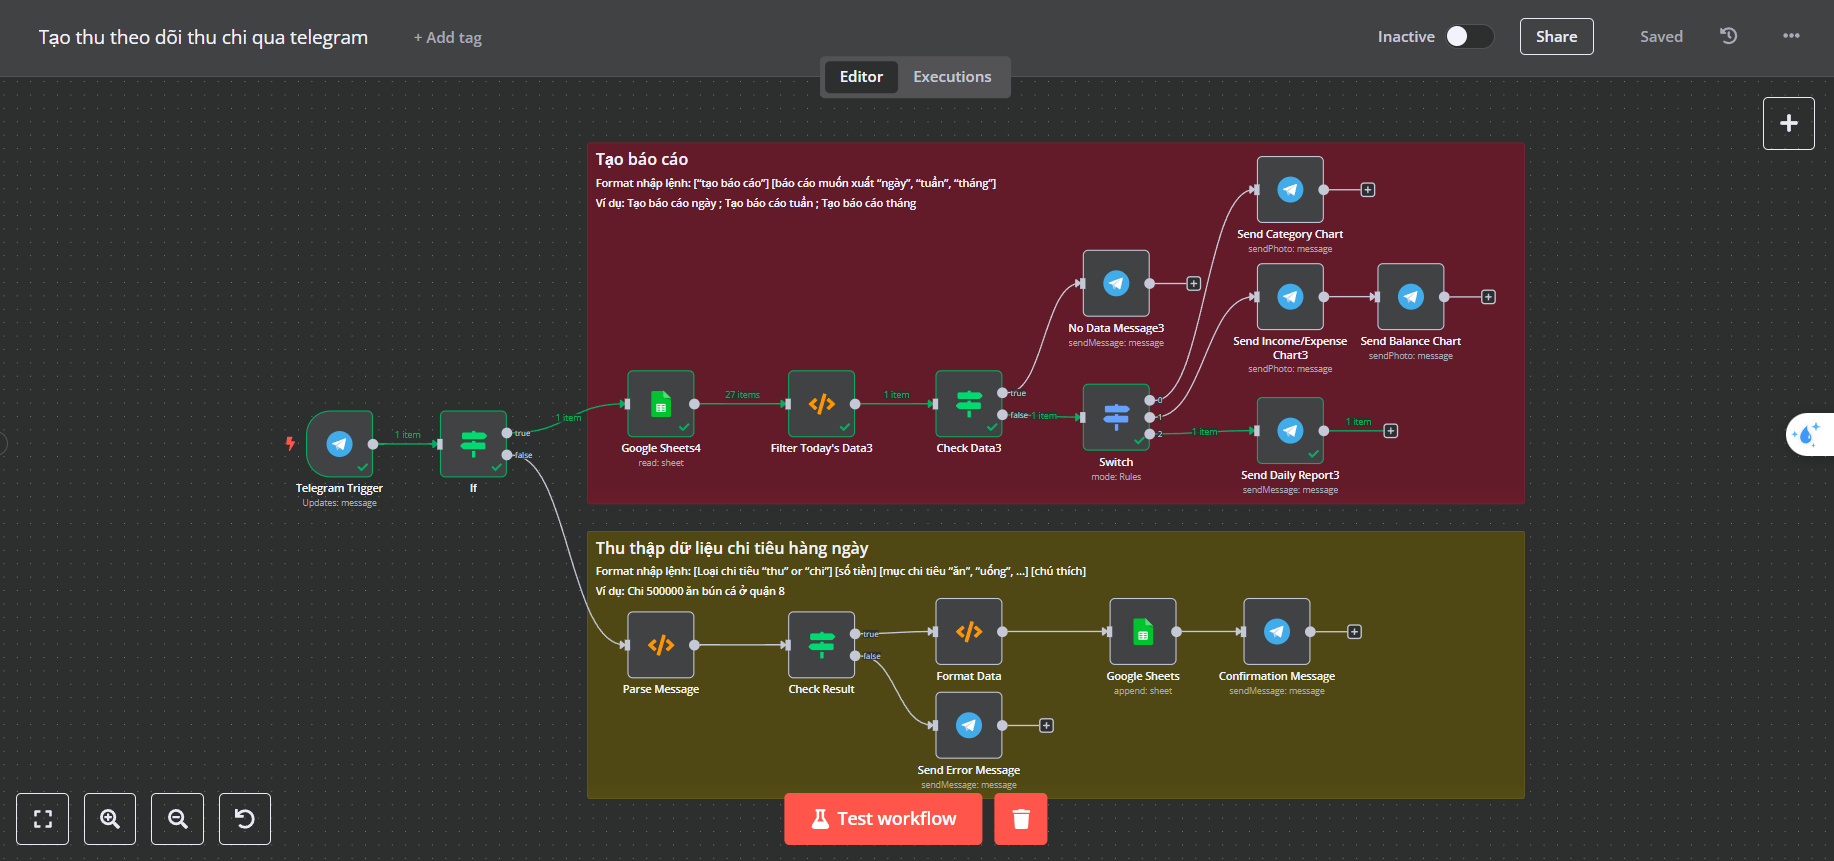
\includegraphics[width=1\textwidth]{images/3thuchi01.png}
    \caption{Workflow theo dõi thu chi}
    
\end{figure}

Đây là một workflow phức tạp nhưng rất hữu ích được xây dựng trên nền tảng n8n để theo dõi tài chính cá nhân thông qua một bot Telegram. Bài viết sẽ phân tích chi tiết các thành phần chính, ưu điểm và cách thiết lập.

\subsection{Tổng quan về workflow}

Workflow này tạo ra một bot Telegram cho phép người dùng:
\begin{enumerate}
    \item Ghi lại các khoản thu chi hàng ngày một cách nhanh chóng
    \item Tạo báo cáo tài chính theo ngày, tuần, tháng với biểu đồ trực quan
    \item Lưu trữ dữ liệu vào Google Sheets để dễ dàng theo dõi và phân tích
\end{enumerate}

\subsection{Các thành phần chính}

\subsubsection{Thu thập dữ liệu từ người dùng}
Bot nhận tin nhắn từ người dùng theo các định dạng:
\begin{itemize}
    \item Nhập khoản chi tiêu: \texttt{[thu/chi] [số tiền] [danh mục] [ghi chú]}
    \begin{itemize}
        \item Ví dụ: \texttt{Chi 500000 ăn bún cá ở quận 8}
    \end{itemize}
    \item Yêu cầu báo cáo: \texttt{Tạo báo cáo [ngày/tuần/tháng]}
    \begin{itemize}
        \item Ví dụ: \texttt{Tạo báo cáo tuần}
    \end{itemize}
\end{itemize}

\subsubsection{Lưu trữ dữ liệu}
\begin{itemize}
    \item Sử dụng Google Sheets làm cơ sở dữ liệu
    \item Mỗi giao dịch được ghi lại với các thông tin: ngày tháng, loại (thu/chi), số tiền, danh mục, ghi chú
\end{itemize}

\subsubsection{Phân tích dữ liệu}
\begin{itemize}
    \item Node Function xử lý phức tạp để tính toán tổng thu, tổng chi và số dư
    \item Phân loại chi tiêu theo danh mục
    \item So sánh với tuần trước để thấy xu hướng
    \item Đưa ra gợi ý tiết kiệm
\end{itemize}

\subsubsection{Tạo báo cáo trực quan}
\begin{itemize}
    \item Sử dụng QuickChart.io để tạo 3 loại biểu đồ:
    \begin{itemize}
        \item Biểu đồ cột thể hiện thu/chi của 4 tuần gần nhất
        \item Biểu đồ đường thể hiện biến động số dư
        \item Biểu đồ tròn phân loại chi tiêu theo danh mục
    \end{itemize}
\end{itemize}

\subsection{Luồng hoạt động}

\begin{enumerate}
    \item \textbf{Nhận tin nhắn từ Telegram}: Node Telegram Trigger bắt tin nhắn từ người dùng
    \item \textbf{Phân loại yêu cầu}: If node kiểm tra xem người dùng muốn nhập giao dịch hay tạo báo cáo
    \item \textbf{Xử lý giao dịch mới}:
    \begin{itemize}
        \item Parse Message phân tích tin nhắn của người dùng
        \item Format Data chuẩn hóa dữ liệu
        \item Google Sheets lưu dữ liệu vào bảng tính
        \item Confirmation Message gửi xác nhận đã lưu giao dịch
    \end{itemize}
    \item \textbf{Tạo báo cáo}:
    \begin{itemize}
        \item Google Sheets4 lấy dữ liệu từ bảng tính
        \item Filter Today's Data3 xử lý và phân tích dữ liệu
        \item Check Data3 kiểm tra xem có dữ liệu không
        \item Switch phân loại loại báo cáo (ngày/tuần/tháng)
        \item Các node Send gửi báo cáo và biểu đồ trực quan
    \end{itemize}
\end{enumerate}

\subsection{Ưu điểm của workflow}

\begin{enumerate}
    \item \textbf{Đơn giản hóa việc theo dõi tài chính}: Nhập giao dịch nhanh chóng qua Telegram mà không cần mở ứng dụng phức tạp
    \item \textbf{Tự động hóa phân tích}: Tự động tính toán, phân loại và so sánh dữ liệu
    \item \textbf{Báo cáo trực quan}: Biểu đồ giúp dễ dàng nắm bắt tình hình tài chính
    \item \textbf{Dễ tiếp cận}: Sử dụng Telegram - ứng dụng nhắn tin phổ biến làm giao diện
    \item \textbf{Lưu trữ an toàn}: Dữ liệu được lưu trong Google Sheets, dễ dàng truy cập và sao lưu
    \item \textbf{Đa ngôn ngữ}: Workflow hỗ trợ tiếng Việt, dễ dàng mở rộng cho các ngôn ngữ khác
\end{enumerate}

\subsection{Hướng dẫn thiết lập cho người mới}

\subsubsection{Bước 1: Chuẩn bị tài khoản và công cụ}
\begin{itemize}
    \item Đăng ký tài khoản \href{https://n8n.io}{n8n}
    \item Tạo bot Telegram thông qua \href{https://t.me/botfather}{BotFather}
    
    \begin{figure}[H]
    \centering
    \includegraphics[width=1\textwidth]{images/3thuchi02.png}
    \caption{Tạo token để truy cập HTTP API telegram}
    \end{figure}
    \begin{figure}[H]
    \centering
    \includegraphics[width=1\textwidth]{images/3thuchi03.png}
    \caption{Tạo token để truy cập HTTP API telegram}
    \end{figure}

- Sau khi Tạo token để truy cập HTTP API telegram, chúng ta sẽ được dãi token như hình trên. \\

- Tạo credential telegram: Nhập dải token vào Access Token, và base URL \texttt{https://api.telegram.org}

    
    \begin{figure}[H]
    \centering
    \includegraphics[width=1\textwidth]{images/3thuchi04.png}
    \caption{Tạo Credential telegram}
    \end{figure}
    
    \item Chuẩn bị một Google Sheet với các cột: date, type, amount, category, note, timestamp
    \begin{figure}[H]
    \centering
    \includegraphics[width=1\textwidth]{images/3thuchi05.png}
    \caption{Form Google sheet lưu trữ thông tin chi tiêu}
    \end{figure}
    
\end{itemize}

- \textbf{\underline{Cài đặt Credeential Google sheet.}}\\
    \begin{figure}[H]
    \centering
    \includegraphics[width=1\textwidth]{images/3thuchi06.png}
    \caption{Tạo dự án Google Cloud Console}
    \end{figure}
$\longrightarrow$ Đăng nhập vào \url{https://console.cloud.google.com/} $\longrightarrow$ Tạo dự án mới
 
    \begin{figure}[H]
    \centering
    \includegraphics[width=1\textwidth]{images/3thuchi07.png}
    \caption{Enable APIs}
    \end{figure}

    \begin{figure}[H]
    \centering
    \includegraphics[width=1\textwidth]{images/3thuchi08.png}
    \caption{Enable APIs}
    \end{figure}
$\longrightarrow$ Chọn đúng tên dự án vừa tạo $\longrightarrow$ truy cập APIs and Services $>$ Library $\longrightarrow$ bật enable cho ứng dụng google mà bạn muốn phân quyền cho n8n truy cập.
    
    \begin{figure}[H]
    \centering
    \includegraphics[width=1\textwidth]{images/3thuchi09.png}
    \caption{Configure your OAuth consent screen}
    \end{figure}

    \begin{figure}[H]
    \centering
    \includegraphics[width=1\textwidth]{images/3thuchi14.png}
    \caption{Configure your OAuth consent screen}
    \end{figure}

    \begin{figure}[H]
    \centering
    \includegraphics[width=1\textwidth]{images/3thuchi16.png}
    \caption{Configure your OAuth consent screen}
    \end{figure}
    
    \begin{figure}[H]
    \centering
    \includegraphics[width=1\textwidth]{images/3thuchi17.png}
    \caption{Configure your OAuth consent screen}
    \end{figure}
    
$\longrightarrow$ Thiết lập OAuth consent screen như hình bên trên.
    
    \begin{figure}[H]
    \centering
    \includegraphics[width=1\textwidth]{images/3thuchi10.png}
    \caption{Create your Google OAuth client credentials}
    \end{figure}
    
$\longrightarrow$ Tìm dấu 3 gạch $\longrightarrow$ API and services $\longrightarrow$ Identifiers $\longrightarrow$ Nhấn vào Create credentials $\longrightarrow$ Oauth client ID $\longrightarrow$ chọn Web application $\longrightarrow$ đặt tên $\longrightarrow$ Allowed redirect URIs: nhập Url trong mục OAuth Redirect URL của n8n

    
    \begin{figure}[H]
    \centering
    \includegraphics[width=1\textwidth]{images/3thuchi11.png}
    \caption{Create your Google OAuth client credentials}
    \end{figure}


    








\textbf{OAuth Redirect URL:} \\
\texttt{https://n8n.haismartlife.com/rest/oauth2-credential/callback}\\
$\longrightarrow$ Cho phép URL này truy cập vào ứng dụng google.\\
\textbf{Grant Type:} Authorization Code\\
\textbf{Authorization URL:}\\
\texttt{https://accounts.google.com/o/oauth2/v2/auth}\\
\textbf{Access Token URL:}\\
\texttt{https://oauth2.googleapis.com/token}\\
\textbf{Client ID:} \\
\verb|434746499575-9oe8fertj8hnqbns8rdk28abs0vivel5.apps.....|\\
$\longrightarrow$ Lấy từ OAuth 2.0 Client IDs tạo ở trên\\
\textbf{Client Secret:}\\
$\longrightarrow$ Lấy từ OAuth 2.0 Client IDs tạo ở trên
    \begin{figure}[H]
    \centering
    \includegraphics[width=1\textwidth]{images/3thuchi12.png}
    \caption{Tạo Credential telegram}
    \end{figure}
\textbf{Auth URI Query Parameters:}\\
\verb|access_type=offline&prompt=consent|
    \begin{figure}[H]
    \centering
    \includegraphics[width=1\textwidth]{images/3thuchi15.png}
    \caption{Tạo Credential telegram}
    \end{figure}
\textbf{Authentication:} Header\\




\subsubsection{Bước 2: Cấu hình webhook và kết nối API}
\begin{enumerate}
    \item Cài đặt credentials cho Telegram API trong n8n
    \item Cấu hình OAuth cho Google Sheets
    \item Thiết lập webhook cho Telegram Trigger
\end{enumerate}

\subsubsection{Bước 3: Tạo cấu trúc workflow}
\begin{enumerate}
    \item Bắt đầu với Telegram Trigger
    \item Thêm If node để phân loại yêu cầu
    \item Tạo nhánh xử lý nhập giao dịch
    \item Tạo nhánh tạo báo cáo
\end{enumerate}

\subsubsection{Bước 4: Cấu hình chi tiết cho từng node}
\begin{enumerate}
    \item \textbf{Parse Message}: Copy code JavaScript từ workflow mẫu để xử lý tin nhắn
    \item \textbf{Filter Today's Data3}: Copy code để phân tích và tạo biểu đồ  
    \item \textbf{Google Sheets}: Cấu hình kết nối với bảng tính của bạn
    \item \textbf{Send nodes}: Điều chỉnh định dạng tin nhắn và caption cho phù hợp
\end{enumerate}

\subsubsection{Bước 5: Kiểm tra và tối ưu}
\begin{enumerate}
    \item Chạy thử workflow với các loại tin nhắn khác nhau
    \item Kiểm tra xem dữ liệu có được lưu chính xác không
    \item Điều chỉnh các định dạng báo cáo và biểu đồ theo nhu cầu
\end{enumerate}

\subsection{Khả năng mở rộng}

Workflow này có thể được mở rộng với các tính năng:
\begin{enumerate}
    \item Thêm báo cáo theo quý/năm
    \item Tạo hệ thống ngân sách và cảnh báo khi vượt quá ngân sách
    \item Thêm chức năng xuất báo cáo dưới dạng PDF
    \item Thêm nhắc nhở thanh toán định kỳ
    \item Tích hợp với các API tài chính để tự động cập nhật giao dịch
\end{enumerate}

\subsection{Kết luận}

Với workflow này, việc theo dõi tài chính cá nhân trở nên đơn giản và trực quan hơn, giúp người dùng dễ dàng nắm bắt tình hình tài chính và đưa ra các quyết định tài chính thông minh hơn. Đây là một ví dụ điển hình về cách n8n có thể được sử dụng để tự động hóa và tối ưu các tác vụ trong cuộc sống hàng ngày mà không cần đến kỹ năng lập trình phức tạp.

\clearpage
%----------------------------------------------------------------
\section{\textbf{Dự án 3: Tạo trợ lý ảo bằng Telegram }}

\href{https://drive.google.com/drive/folders/1-qVA3yQnfIx70DsZKdPAGYQcr8WftkGJ?usp=sharing}{\textbf{\underline {Link tải workflow}}}

    \begin{figure}[H]
    \centering
    \includegraphics[width=1\textwidth]{images/4chatbot01.png}
    \caption{Workflow trợ lý ảo Telegram}
    \end{figure}


\subsection{Phân tích chi tiết công dụng và ưu điểm}

\subsubsection{Công dụng chính}
\begin{enumerate}
    \item \textbf{Trợ lý đa chức năng tự động}: Hệ thống hoạt động như một trợ lý cá nhân/văn phòng tự động xử lý nhiều loại tác vụ khác nhau.
    
    \item \textbf{Tích hợp đa nền tảng}: Kết nối Telegram làm giao diện người dùng với các dịch vụ Gmail, Google Calendar, Airtable và công cụ tìm kiếm.
    
    \item \textbf{Xử lý ngôn ngữ tự nhiên}: Người dùng có thể giao tiếp bằng văn bản hoặc giọng nói tự nhiên, không cần câu lệnh cụ thể.
    
    \item \textbf{Tự động hóa công việc hàng ngày}:
    \begin{itemize}
        \item Quản lý email: gửi, lấy, dán nhãn, tạo bản nháp
        \item Quản lý lịch: tạo, xóa, cập nhật sự kiện và cuộc họp
        \item Quản lý danh bạ: lưu trữ và truy xuất thông tin liên hệ
        \item Tạo nội dung: viết và xuất bản bài blog dựa trên nghiên cứu
    \end{itemize}
\end{enumerate}

\subsubsection{Ưu điểm nổi bật}
\begin{enumerate}
    \item \textbf{Kiến trúc module hóa}: Mỗi chức năng được phân tách thành agent riêng biệt, dễ bảo trì và mở rộng.
    
    \item \textbf{Tự động định tuyến tác vụ}: Hệ thống tự nhận diện yêu cầu và chuyển đến agent phù hợp.
    
    \item \textbf{Sử dụng LLM tiên tiến}: OpenRouter và OpenAI đảm bảo khả năng hiểu và xử lý ngôn ngữ tự nhiên chất lượng cao.
    
    \item \textbf{Xử lý lỗi thông minh}: Các agent đều có xử lý lỗi (error handling) để đảm bảo trải nghiệm người dùng mượt mà.
    
    \item \textbf{Cá nhân hóa cao}: Kết nối với tài khoản cá nhân của người dùng (email, lịch, danh bạ).
    
    \item \textbf{Đa dạng đầu vào}: Xử lý cả tin nhắn văn bản và ghi âm, tăng tính linh hoạt.
    
    \item \textbf{Tương tác hai chiều}: Cung cấp phản hồi kịp thời qua tin nhắn hoặc file âm thanh.
\end{enumerate}

\subsection{Hướng dẫn thiết lập credentials}

\subsubsection{Tổng quan về credentials cần thiết}
Để thiết lập toàn bộ hệ thống chatbot Ultimate Assistant, bạn cần cấu hình các xác thực (credentials) cho các dịch vụ sau:

\begin{itemize}
    \item Telegram Bot API
    \item OpenAI/OpenRouter API
    \item Google (Gmail và Calendar)
    \item Airtable
    \item Tavily Search API
\end{itemize}

Dưới đây là hướng dẫn chi tiết cách thiết lập từng loại credential:

\subsubsection{\underline{Telegram Bot API}}
\textbf{Mục đích}: Cho phép chatbot tương tác với người dùng qua Telegram.

\textbf{Cách thiết lập}:
\begin{enumerate}
    \item Mở Telegram và tìm kiếm \texttt{\href{https://telegram.me/BotFather}{@BotFather}}
    \item Gửi lệnh \texttt{/newbot} và làm theo hướng dẫn để tạo bot mới
    \item Đặt tên cho bot và username (phải kết thúc bằng ``bot'')
    \item BotFather sẽ cung cấp token API (dạng \texttt{123456789:ABCdefGhIJKlmNoPQRsTUVwxyZ})
    \item Trong n8n:
    \begin{itemize}
        \item Vào ``Credentials'' > ``New'' > ``Telegram API''
        \item Nhập Bot Token API đã nhận được
        \item Lưu credential với tên (ví dụ: ``Telegram account Hai'')
    \end{itemize}
\end{enumerate}

\subsubsection{\underline{OpenAI/OpenRouter API}}
\textbf{Mục đích}: Cung cấp mô hình ngôn ngữ (LLM) để chatbot hiểu và tạo phản hồi.

\paragraph{OpenAI API:}
\begin{enumerate}
    \item Đăng ký tài khoản tại \href{https://platform.openai.com/}{OpenAI}
    \item Truy cập ``API Keys'' và tạo key mới
    \item Trong n8n:
    \begin{itemize}
        \item Vào ``Credentials'' > ``New'' > ``OpenAI API''
        \item Nhập API Key
        \item Lưu credential với tên (ví dụ: ``OpenAi account'')
    \end{itemize}
\end{enumerate}

\paragraph{OpenRouter API} (thay thế cho OpenAI): thay đổi nhiều model LLM 
\begin{enumerate}
    \item Đăng ký tại \href{https://openrouter.ai/}{OpenRouter}
    \item Tạo API key mới
    \item Trong n8n:
    \begin{itemize}
        \item Vào ``Credentials'' > ``New'' > ``OpenRouter API''
        \item Nhập API Key
        \item Lưu credential với tên (ví dụ: ``OpenRouter account'')
    \end{itemize}
\end{enumerate}

\subsubsection{\underline{Google (Gmail và Calendar)}}
\textbf{Mục đích}: Cho phép chatbot truy cập và quản lý email và lịch.

\textbf{Thiết lập Google OAuth2}:
\begin{enumerate}
    \item Truy cập \href{https://console.cloud.google.com/}{Google Cloud Console}
    \item Tạo project mới hoặc chọn project sẵn có
    \item Đi tới ``APIs \& Services'' > ``Library''
    \item Kích hoạt các API: Gmail API và Google Calendar API
    \item Đi tới ``OAuth consent screen'':
    \begin{itemize}
        \item Chọn loại người dùng (External/Internal)
        \item Nhập thông tin ứng dụng (tên, email liên hệ)
        \item Thêm scopes cần thiết: Gmail (send, read, modify) và Calendar (read, write)
    \end{itemize}
    \item Tạo OAuth2 credentials:
    \begin{itemize}
        \item Đi tới ``Credentials'' > ``Create Credentials'' > ``OAuth client ID''
        \item Chọn Application Type: ``Web application''
        \item Thêm Redirect URI: URL từ n8n (thường có dạng \url{https://your-n8n-instance.com/rest/oauth2-credential/callback})
    \end{itemize}
    \item Trong n8n:
    \begin{itemize}
        \item Vào ``Credentials'' > ``New'' > ``OAuth2 API'' (cho Gmail hoặc Google Calendar)
        \item Nhập Client ID và Client Secret từ Google Cloud
        \item Nhập các scopes cần thiết
        \item Nhấn ``Connect'' và xác thực với tài khoản Google của bạn
        \item Lưu credentials với tên phù hợp (ví dụ: ``Gmail account'', ``Google Calendar account'')
    \end{itemize}
\end{enumerate}

\subsubsection{\underline{Airtable}}
\textbf{Mục đích}: Lưu trữ và quản lý thông tin liên hệ.

\textbf{Thiết lập Airtable API}:
\begin{enumerate}
    \item Đăng nhập vào \href{https://airtable.com/}{Airtable}
    \item Tạo một base mới với bảng ``Contacts'' chứa các trường: name, email, phoneNumber
    \item Truy cập ``Account'' > ``Developer Hub'' > ``Personal Access Tokens''
    \item Tạo token mới với quyền truy cập phù hợp
    \item Trong n8n:
    \begin{itemize}
        \item Vào ``Credentials'' > ``New'' > ``Airtable API''
        \item Nhập API Key
        \item Lưu credential với tên phù hợp
    \end{itemize}
    \item Lấy Base ID:
    \begin{itemize}
        \item Mở Airtable base của bạn
        \item Xem URL: \texttt{https://airtable.com/[BASE\_ID]/[TABLE\_ID]/[VIEW\_ID]}
        \item Lưu lại BASE\_ID để sử dụng trong workflow
    \end{itemize}
\end{enumerate}

\subsubsection{\underline{Tavily Search API}}
\textbf{Mục đích}: Cho phép chatbot tìm kiếm thông tin trên web.

\textbf{Thiết lập Tavily API}:
\begin{enumerate}
    \item Đăng ký tài khoản tại \href{https://tavily.com/}{Tavily}
    \item Nhận API key từ dashboard
    \item Trong workflow n8n:
    \begin{itemize}
        \item Tại nút HTTP Request Tool, nhập trực tiếp API key vào JSON body:
    \end{itemize}
\end{enumerate}

\begin{lstlisting}[language=json, basicstyle=\small\ttfamily]
{
  "api_key": "tvly-YOUR_API_KEY",
  "query": "{searchTerm}",
  "search_depth": "basic",
  "include_answer": true,
  "topic": "news",
  "include_raw_content": true,
  "max_results": 3
}
\end{lstlisting}

\subsubsection{\underline{Kiểm tra và xác minh credentials}}
Sau khi cài đặt tất cả credentials:
\begin{itemize}
    \item Kiểm tra từng workflow để đảm bảo nó được liên kết với credential đúng
    \item Thực hiện kiểm tra kết nối cho mỗi credential trong n8n
    \item Chạy thử từng workflow thành phần trước khi tích hợp vào hệ thống chính
\end{itemize}

\subsubsection{\underline{Lưu ý bảo mật}}
\begin{itemize}
    \item \textbf{Không chia sẻ API keys}: Bảo vệ tất cả credentials và không chia sẻ trong code công khai
    \item \textbf{Giới hạn quyền truy cập}: Chỉ cấp quyền cần thiết cho mỗi API
    \item \textbf{Theo dõi sử dụng}: Giám sát việc sử dụng API để tránh vượt quá giới hạn
    \item \textbf{Luân chuyển keys}: Cập nhật keys định kỳ theo các thực hành bảo mật tốt nhất
    \item \textbf{Mã hóa credentials}: n8n mã hóa credentials, nhưng hãy đảm bảo máy chủ n8n được bảo mật
\end{itemize}

Với tất cả các credentials được thiết lập đúng cách, Ultimate Assistant Chatbot của bạn sẽ có thể tương tác với Telegram và điều phối tất cả các dịch vụ bên ngoài một cách liền mạch.

\clearpage
%----------------------------------------------------------------------
\section{\textbf{Dự án 4: Tạo short video hoạt hình bằng AI và đăng lên youtube }}

\href{https://drive.google.com/file/d/1hBEgM7DZBiMOocM_pxGyne7T97oAKK_B/view?usp=sharing}{\textbf{\underline {Link tải workflow}}}

\begin{figure}[h]
    \centering
    \includegraphics[width=1\textwidth]{images/Da1-01.png}
    \caption{Workflow kết quả dự án 1}
    
\end{figure}

Trong ví dụ này chúng ta sẽ làm một workflow để tạo short video animated. \\

\underline{Ứng dụng:}\\
\begin{itemize}[label=-]
    \item Nhà tiếp thị muốn tạo video quảng cáo tự động, nhanh chóng
    \item Người sáng tạo nội dung muốn tối ưu hóa quy trình sản xuất video
    \item Doanh nghiệp tìm kiếm phương pháp hiệu quả để giới thiệu sản phẩm 
\end{itemize}


\underline{Ý tưởng thiết kế:}\\
\begin{figure}[h]
    \centering
    \includegraphics[width=0.7\textwidth]{images/Da1-02.png}
    \caption{Ý tưởng thiết kế}
    
\end{figure}


\underline{Các công cụ sử dụng trong workflow:}\\
\begin{itemize}[label=-]
    \item \textbf{Tạo giọng nói AI với ElevenLabs}: Sử dụng \textbf{\emph{ElevenLabs}}, quy trình này chuyển đổi văn bản thành giọng nói tự nhiên, giúp video trở nên sống động và chuyên nghiệp hơn. ElevenLabs AI là một nền tảng AI Text-to-Speech (TTS) giúp chuyển đổi văn bản thành giọng nói tự nhiên, chân thực với nhiều giọng đọc và ngôn ngữ khác nhau. Nó thường được dùng để tạo giọng nói nhân tạo phục vụ video, podcast, ứng dụng AI, chatbot và nhiều mục đích khác. ElevenLabs AI giúp tự động hóa quy trình tạo giọng nói từ văn bản. Dùng trong một số ứng dụng thực tế như: Chuyển đổi văn bản thành giọng nói (TTS) tự động, Tạo chatbot có giọng nói nhân tạo, Đọc báo, thông tin hoặc tin tức tự động, Tổng đài AI tự động (Voice AI Callbot)
    \item \textbf{Chuyển đổi ảnh thành video với Hailuo AI}: Với  \textbf{\emph{Hailuo AI}} hình ảnh tĩnh được chuyển đổi thành video động, giúp tạo nội dung trực quan hấp dẫn mà không cần chỉnh sửa thủ công. Các ứng dụng mà Hailou AI có thể làm.\\

    + Chuyển đổi văn bản thành video: Hailuo AI giúp biến những đoạn văn bản thành video sống động, tối ưu hóa quy trình sáng tạo nội dung và tiết kiệm thời gian cho người dùng.\\
    + Chuyển đổi hình ảnh thành video: Người dùng có thể tải lên hình ảnh tĩnh và nhập mô tả; Hailuo AI sẽ tạo ra video dựa trên nội dung đó, mang lại trải nghiệm trực quan và sinh động.\\
    + Chuyển đổi văn bản thành giọng nói (Text-to-Speech): Hailuo AI cung cấp tính năng chuyển đổi văn bản thành giọng nói với nhiều ngôn ngữ và giọng đọc tự nhiên, hỗ trợ đa dạng nhu cầu của người dùng. 
    \item \textbf{Cải thiện nội dung với Together AI}: Để đảm bảo chất lượng nội dung cao, \textbf{\emph{Together AI}} tối ưu hóa và điều chỉnh lời nhắc, giúp tạo ra các kịch bản hấp dẫn và phù hợp hơn. Nó giống một bên trung gian để chung ta truy cập vào các mô hình AI.
    \item \textbf{Xử lý thông minh với OpenAI}: Các tác vụ suy luận, như tạo nội dung văn bản và tối ưu hóa nội dung, được thực hiện bởi \textbf{\emph{OpenAI}}, giúp quy trình sản xuất video diễn ra trơn tru và hiệu quả. 
    \item \textbf{Tích hợp với Google Sheets}: Sau khi tạo video, \textbf{\emph{URL tải xuống}} sẽ được tự động tải lên \textbf{\emph{Google Sheets}}, giúp người dùng dễ dàng truy cập và quản lý nội dung. 
     \item \textbf{Lưu trữ thông tin bằng Google Cloud Storage}: Node \textbf{\emph{Google Cloud Storage}} trong n8n giúp bạn làm việc với dịch vụ lưu trữ đám mây Google Cloud Storage (GCS). Nó cho phép bạn tải lên, tải xuống, xóa và quản lý tệp trên Google Cloud Storage Buckets trong quy trình tự động hóa của mình. 
     \item \textbf{Tối ưu hóa với node code}: Node Code trong n8n cho phép bạn viết JavaScript để xử lý dữ liệu tùy chỉnh trong quy trình tự động hóa. Nó giúp mở rộng khả năng của n8n khi các node có sẵn không đáp ứng đủ nhu cầu.   
\end{itemize}

\underline{\textbf{ Các bước triển khai:}}

\subsection{Tạo node "Edit Fields}

\begin{itemize}
    \item[-] Tạo các trường dữ liệu (data fields): Node Edit File cho phép tạo ra các trường dữ liệu mới và gán giá trị cho chúng.
    \item[-] Mapping (ánh xạ) dữ liệu: Node Edit File được sử dụng để ánh xạ dữ liệu từ các nguồn khác nhau và kết hợp chúng lại với nhau. Ví dụ: Ánh xạ URL của audio đã tạo, Kết hợp URL của video và nhạc nền. Thiết lập các tham số (parameters): Node Edit File được sử dụng để thiết lập các tham số cần thiết cho các bước tiếp theo trong quy trình.
    \item[-] Chỉnh sửa thông tin: Node Edit File có thể chỉnh sửa các thông tin khác nhau.
\end{itemize}  
    \begin{figure}[H]
 
    \centering
    \begin{minipage}{0.5\textwidth}
        \includegraphics[width=\linewidth]{images/Da1-03.png}
    \end{minipage}
    %\hfill
    \hspace{5pt}
    \begin{minipage}{0.4\textwidth}
    
        \underline{Các thông số cần cài đặt:}\\
        \begin{itemize}[label=\textbullet]
            \item Đổi tên node thành \emph{"Video Catagory"}
            \item Mục Mode: Chọn \emph{"Manual Mapping"}
            \item Mục Fields to Set: Chọn "Add Field" và tạo 3 trường như hình bên cạnh, trong đó:\\
            
            \textbf{\emph{"Video Category"}} là trường  nội dung video bạn muốn tạo, thay thế thành loại video hoặc nội dung bạn muốn.\\
            \textbf{\emph{"Bucket Name"}} là tên của bucket mà bạn sẽ tạo trong google cloud để lưu các hình ảnh, âm thanh AI tạo ra.\\
            \textbf{\emph{"Unique ID"}} bằng giá trị "\verb|{{$now.valueOf()}}|" là một tham số quan trọng để đảm bảo tính duy nhất và chính xác của các tệp trong quy trình tạo video tự động, đặc biệt là để ngăn chặn các vấn đề liên quan đến caching.\\

            
        \end{itemize}
    \end{minipage}
\end{figure}
     
    % \item 
    % \item 
    % \item 
    % \item 


\subsection{Elevenlabs - AI về âm thanh, chuyển đổi text và voice.}
\begin{itemize}[label=]
    \item \textbf{Bước 1: Tạo API key Elevenlabs} 
    
    Truy cập vào link \url{https://elevenlabs.io/app/settings/api-keys} \\ 
    
    Tìm đến API key và nhấn tạo ta sẽ được dãy ký tự, sau đó hãy copy nó.\\
    
    Lưu ý: API này dùng free sẽ hay bị lỗi nên nếu xây dựng được một workflow hữu ích thì nên mua để tránh gặp các lỗi không mong muốn.\\
    
    \begin{figure}[H]
    \centering
    \includegraphics[width=1.0\textwidth]{images/Elevenlabs.pdf}
    \caption{Tạo API Elevenlabs}
    
    \end{figure}
 Tạo được API có dạng " sk\_7529a9c2502bb52789fa8cfcdafdc645c5edc038244e3136 " \\
 
    \begin{figure}[H]
    \centering
    \includegraphics[width=0.6\textwidth]{images/Elevenlabs-1.pdf}
    \caption{Tạo API Elevenlabs}
    
    \end{figure}

    \item \textbf{Bước 2: Tạo node "HTTP truy cập Elevenlabs" trong n8n}\\
    
    \begin{figure}[h]
 
    \centering
    \begin{minipage}{0.45\textwidth}
        \includegraphics[width=\linewidth]{images/Elevenlabs-2.pdf}
    \end{minipage}
    %\hfill
    \hspace{5pt}
    \begin{minipage}{0.45\textwidth}
         \includegraphics[width=\linewidth]{images/Elevenlabs-3.pdf}
    \end{minipage}
\end{figure}

Tại mục URL nhập: \\
"https://api.elevenlabs.io/v1/text-to-speech/N2lVS1w4EtoT3dr4eOWO"\\

Trong đó "N2lVS1w4EtoT3dr4eOWO" chính là ID của giọng nói mà các bạn muốn xuất hiện trong video

 \begin{figure}[H]
    \centering
    \includegraphics[width=1\textwidth]{images/Elevenlabs-4.pdf}
    \caption{Tạo API Elevenlabs}
    
    \end{figure}

 \begin{figure}[H]
    \centering
    \includegraphics[width=1\textwidth]{images/Elevenlabs-5.png}
    \caption{Tạo API Elevenlabs}
    
    \end{figure}
    Set up credential cho Elevenlabs như hình bên dưới:\\
    Name: xi-api-key\\
    Value: " sk\_7529a9c2502bb52789fa8cfcdafdc645c5edc038244e3136 " (Paste API copy từ web Elevenlabs) \\

\end{itemize}

%--------------------------------------------------------------

\subsection{Together AI - nền tảng hỗ trợ các module AI tối ưu kết quả.}
\begin{itemize}[label=]
    \item \textbf{Bước 1: Tạo API key Together AI} 
    
    Truy cập vào link \url{https://api.together.ai/settings/api-keys} \\ 
    Tìm đến API keys và copy nó ta sẽ được dãy ký tự.\\
    Lưu ý: Thêm thông tin thẻ thanh toán và sử dụng như thường, và có thể thay node này bằng node khác có chức năng tương đương thể thử.\\
    
    \begin{figure}[H]
    \centering
    \includegraphics[width=0.95\textwidth]{images/TogetherAI.png}
    \caption{Tạo API Together AI}
    
    \end{figure}
    \item \textbf{Bước 2: Tạo node "HTTP truy cập Together AI" trong n8n}\\
    \begin{figure}[H]
    \centering
    \includegraphics[width=0.95\textwidth]{images/TogetherAI-1.png}
    \caption{Tạo API Together AI}
    
    \end{figure}
    
 Tạo Node HTTP trong n8n, trong phần Header Auth chúng ta tạo credential như hình trên:\\
 Name: authorization\\
 Value: API vừa copy ở web Together AI\\
 
    \begin{figure}[H]
    \centering
    \begin{minipage}{0.45\textwidth}
        \includegraphics[width=\linewidth]{images/TogetherAI-2.png}
    \end{minipage}
    %\hfill
    \hspace{5pt}
    \begin{minipage}{0.45\textwidth}
         \includegraphics[width=\linewidth]{images/TogetherAI-3.png}
    \end{minipage}
\end{figure}

Tại mục URL nhập: \\
"https://api.together.xyz/v1/chat/completions"\\


\end{itemize}

%------------------------------------------------------
\subsection{Google cloud storage - Lưu trữ các video, Audio, Hình ảnh tạo ra}
\begin{itemize}[label=]
    \item \textbf{Bước 1: Set up tài khoản} 
    
    Truy cập vào link \url{https://console.cloud.google.com/} \\ 

    \begin{figure}[H]
    \centering
    \includegraphics[width=0.95\textwidth]{images/GGcloud.png}
    
    \end{figure}
    \begin{figure}[H]
    \centering
    \includegraphics[width=0.95\textwidth]{images/GGcloud-1.png}
    
    \end{figure}
    
    \begin{figure}[H]
    \centering
    \includegraphics[width=0.95\textwidth]{images/GGcloud-2.png}
    
    \end{figure}
    \begin{figure}[H]
    \centering
    \includegraphics[width=0.95\textwidth]{images/GGcloud-3.png}

    \end{figure}
    \begin{figure}[H]
    \centering
    \includegraphics[width=0.95\textwidth]{images/GGcloud-4.png}
    
    \end{figure}
    \begin{figure}[H]
    \centering
    \includegraphics[width=0.95\textwidth]{images/GGcloud-5.png}
    
    \end{figure}
    \begin{figure}[H]
    \centering
    \includegraphics[width=0.95\textwidth]{images/GGcloud-6.png}
    
    \end{figure}
    \begin{figure}[H]
    \centering
    \includegraphics[width=0.95\textwidth]{images/GGcloud-7.png}
    
    \end{figure}
    \begin{figure}[H]
    \centering
    \includegraphics[width=0.95\textwidth]{images/GGcloud-8.png}
    
    \end{figure}
    \begin{figure}[H]
    \centering
    \includegraphics[width=0.95\textwidth]{images/GGcloud-9.png}
    
    \end{figure}
    \begin{figure}[H]
    \centering
    \includegraphics[width=0.95\textwidth]{images/GGcloud-10.png}
    
    \end{figure}
        \begin{figure}[H]
    \centering
    \includegraphics[width=0.95\textwidth]{images/GGcloud-11.png}
    
    \end{figure}
    \begin{figure}[H]
    \centering
    \includegraphics[width=0.95\textwidth]{images/GGcloud-12.png}
    
    \end{figure}

    \begin{figure}[H]
    \centering
    \includegraphics[width=0.95\textwidth]{images/GGcloud-14.png}
    
    \end{figure}
    \begin{figure}[H]
    \centering
    \includegraphics[width=0.95\textwidth]{images/GGcloud-15.png}
    
    \end{figure}

    \begin{figure}[H]
    \centering
    \includegraphics[width=0.95\textwidth]{images/GGcloud-13.png}
    
    \end{figure}


    
    \item \textbf{Bước 2: Tạo node "Google cloud storage" trong n8n}\\
    \begin{figure}[H]
    \centering
    \includegraphics[width=0.95\textwidth]{images/GGcloud-16.png}
    
    \end{figure}
    
 Tạo Node HTTP trong n8n, trong phần Header Auth chúng ta tạo credential như hình trên:\\
 Name: authorization\\
 Value: API vừa copy ở web Together AI\\
     \begin{figure}[H]
    \centering
    \includegraphics[width=0.6\textwidth]{images/GGcloud-17.png}
    
    \end{figure}
       \verb|{{ $('Video Catagory').first().json['Bucket Name'] }}|\\
    \verb|Voice-{{ $('Video Catagory').first().json['Unique ID'] }}.mp3|

\end{itemize}

%---------------------------------
\subsection{Hailuo AI - Tạo video bằng Hailuo AI.}
\begin{itemize}[label=]
    \item \textbf{Bước 1: Tạo API key Hailuo AI} 
    
    Truy cập vào link \url{https://hailuoai.video/} \\ 
    Tìm đến API keys và copy nó ta sẽ được dãy ký tự.\\
    Lưu ý: Thêm thông tin thẻ thanh toán và sử dụng như thường, và có thể thay node này bằng node khác có chức năng tương đương thể thử.\\
    
    \begin{figure}[H]
    \centering
    \includegraphics[width=0.95\textwidth]{images/HailuoAI.png}
    \caption{Tạo API Together AI}
    
    \end{figure}
    \item \textbf{Bước 2: Tạo node "HTTP truy cập Together AI" trong n8n}\\
    \begin{figure}[H]
    \centering
    \includegraphics[width=0.95\textwidth]{images/HailuoAI-1.png}
    \caption{Tạo API Elevenlabs}
    
    \end{figure}
    \begin{figure}[H]
    \centering
    \includegraphics[width=0.95\textwidth]{images/HailuoAI-2.png}
    \caption{Tạo API Elevenlabs}
    
    \end{figure}
    
 Tạo Node HTTP trong n8n, trong phần Header Auth chúng ta tạo credential như hình trên:\\
 Name: authorization\\
 Value: Bearer API vừa copy ở web Together AI\\
 

Tại mục URL nhập: \\
"https://api.together.xyz/v1/chat/completions"\\

Tại mục Json nhập: 


Dưới đây là đoạn JSON:\\

Nơi lấy code \url{https://haismartlife.com/}


\end{itemize}


%---------------------------------
\subsection{Andynocode - Combine video.}
\begin{itemize}[label=]
    \item \textbf{Bước 1: Tạo API key Hailuo AI} 
    
    Truy cập vào link \url{https://hailuoai.video/} \\ 
    Tìm đến API keys và copy nó ta sẽ được dãy ký tự.\\
    Lưu ý: Thêm thông tin thẻ thanh toán và sử dụng như thường, và có thể thay node này bằng node khác có chức năng tương đương thể thử.\\
    
    \begin{figure}[H]
    \centering
    \includegraphics[width=0.95\textwidth]{images/Andy02.png}
    \caption{Tạo API Together AI}
    
    \end{figure}
    \item \textbf{Bước 2: Tạo node "HTTP truy cập Together AI" trong n8n}\\
    \begin{figure}[H]
    \centering
    \includegraphics[width=0.95\textwidth]{images/Andy01.png}
    \caption{Tạo API Elevenlabs}
    
    \end{figure}

    
 Tạo Node HTTP trong n8n, trong phần Header Auth chúng ta tạo credential như hình trên:\\
 Name: authorization\\
 Value: Bearer API vừa copy ở web Together AI\\
 

Tại mục URL nhập: \\
"https://api.together.xyz/v1/chat/completions"\\

Tại mục Json nhập: 


Dưới đây là đoạn JSON:\\

Nơi lấy code \url{https://haismartlife.com/}


\end{itemize}


%%%%%% Chương 9
\chapter{Case Study thực tế (phần 2)}

\section{\textbf{Dự án 1: Tạo RAG system - hệ thống trả lời câu hỏi bằng tài liệu người dùng}}

\href{https://drive.google.com/file/d/1SwPcQe6HypodnICqbvVpzWVUKQA8_PLI/view?usp=sharing}{\textbf{\underline {Link tải workflow}}}

\begin{figure}[H]
    \centering
    \includegraphics[width=1\textwidth]{images/1rag01.pdf}
    \caption{Workflow kết quả dự án 1}

\end{figure}

Workflow trong mã nguồn được chia sẻ là một hệ thống RAG (Retrieval Augmented Generation) nâng cao được xây dựng trên nền tảng n8n. Đây là một giải pháp toàn diện cho việc xử lý, lưu trữ và truy vấn thông tin từ nhiều loại tài liệu khác nhau.

\textbf{Chức năng chính:}
\begin{itemize}
    \item \textbf{Tự động xử lý tài liệu:} Phát hiện khi tài liệu mới được tạo hoặc cập nhật trong thư mục Google Drive; Hỗ trợ nhiều định dạng tài liệu: PDF, Google Docs, CSV, Excel, và văn bản thông thường; Tự động trích xuất nội dung từ các loại tài liệu khác nhau.
    
    \item \textbf{Xử lý thông minh dựa trên loại tài liệu:} Văn bản và PDF: Chia nhỏ thành các đoạn có nghĩa, tạo embedding và lưu vào Supabase; Dữ liệu bảng (CSV/Excel): Trích xuất cấu trúc và nội dung, lưu trữ thông tin metadata và dữ liệu hàng.
    
    \item \textbf{Lưu trữ dữ liệu hiệu quả:} Sử dụng bảng \texttt{documents} với vectơ embedding thông qua pgvector; Bảng \texttt{document\_metadata} lưu thông tin về tài liệu; Bảng \texttt{document\_rows} lưu dữ liệu từ các tệp CSV/Excel.
    
    \item \textbf{Giao diện trò chuyện AI thông minh:} API webhook để nhận yêu cầu từ người dùng; Agent AI có thể sử dụng nhiều công cụ khác nhau để trả lời câu hỏi; Hỗ trợ bộ nhớ trò chuyện qua PostgreSQL.
    
    \item \textbf{Khả năng truy vấn đa dạng:} Tìm kiếm tương tự ngữ nghĩa (RAG); Truy vấn SQL trực tiếp trên dữ liệu bảng; Truy xuất toàn bộ nội dung tài liệu khi cần thiết.
\end{itemize}

\textbf{Điểm nổi bật:}
\begin{itemize}
    \item \textbf{Kiến trúc RAG Agent thông minh:} Không chỉ đơn thuần là RAG thông thường, workflow này sử dụng cách tiếp cận "agent" cho phép LLM chọn công cụ phù hợp nhất để trả lời câu hỏi.
    
    \item \textbf{Xử lý tài liệu linh hoạt:} Tự động phát hiện định dạng tài liệu và áp dụng phương pháp xử lý phù hợp, không cần cấu hình riêng cho từng loại tài liệu.
    
    \item \textbf{Tối ưu cho dữ liệu số học:} Sử dụng SQL để thực hiện phân tích chính xác trên dữ liệu bảng, khắc phục hạn chế của RAG tiêu chuẩn với dữ liệu số học.
    
    \item \textbf{Khả năng mở rộng:} Thiết kế dễ dàng mở rộng để hỗ trợ thêm nguồn dữ liệu và công cụ mới.
    
    \item \textbf{Hiệu quả lưu trữ:} Sử dụng JSONB trong Supabase để lưu trữ dữ liệu bảng mà không cần tạo bảng mới cho mỗi tệp CSV.
    
    \item \textbf{Tận dụng công nghệ hiện đại:} Kết hợp pgvector, OpenAI Embeddings, và LLM để tạo hệ thống RAG hoàn chỉnh.
\end{itemize}

\textbf{Hướng dẫn thiết lập:}

\textit{Bước 1: Chuẩn bị cơ sở dữ liệu}
\begin{itemize}
    \item \textbf{Thiết lập Supabase:} Tạo tài khoản Supabase và dự án mới; Lưu thông tin kết nối: URL và API Key.
    \begin{figure}[H]
    \centering
    \includegraphics[width=1\textwidth]{images/1rag05.pdf}
    \caption{Thông tin Credential của Supabase}
    \end{figure}
    
    \item \textbf{Thiết lập PostgreSQL:} Đảm bảo PostgreSQL được cài đặt và hỗ trợ pgvector; Chạy các node tạo bảng theo thứ tự: \texttt{Create Documents Table and Match Function}, \texttt{Create Document Metadata Table}, \texttt{Create Document Rows Table}. Chạy 3 node này để tạo bảng và gọi thư viện tạo vector trong Supabase.\\
    \begin{figure}[H]
\centering
\includegraphics[width=1\textwidth]{images/1rag06.pdf}
\caption{Thông tin Credential của Postgres}
\end{figure}
Password của Postgres chính là mật khẩu lúc khởi tạo dự án. Nếu quên mật khẩu có thể vào cài đặt - Database - Database password và đặt lại. \\

Luu ý: phải chạy 3 node postgres trước khi upload file lên googledrive, để tạo bảng và khởi tạo biến vector trước. Nếu không sẽ bị lỗi và không chạy được\\

\end{itemize}
    

    
\begin{figure}[H]
\centering
\includegraphics[width=1\textwidth]{images/1rag07.pdf}
\caption{Thông tin Credential của Postgres}
\end{figure}
    
    

\textit{Bước 2: Cấu hình Google Drive}
\begin{itemize}
    \item \textbf{Thiết lập OAuth:} Tạo OAuth credentials trong Google Developer Console; Thêm thông tin xác thực vào n8n.
    
    \item \textbf{Cấu hình thư mục:} Tạo thư mục riêng để chứa tài liệu cho bot; Lấy ID thư mục và cấu hình trong các node \texttt{File Created} và \texttt{File Updated}.
\end{itemize}

\textit{Bước 3: Cấu hình OpenAI API}
\begin{itemize}
    \item \textbf{Tạo API key:} Đăng ký tài khoản và tạo API key từ OpenAI; Thêm thông tin xác thực vào n8n.
    
    \item \textbf{Cấu hình model:} Cấu hình mô hình embeddings (text-embedding-3-small); Cấu hình mô hình chat (gpt-4 hoặc tương tự).
\end{itemize}

\textit{Bước 4: Thiết lập Workflow}
\begin{itemize}
    \item \textbf{Xử lý tài liệu:} Cấu hình node trigger với ID thư mục Google Drive; Thiết lập các node xử lý tài liệu; Cấu hình node \texttt{Switch} để định tuyến luồng dữ liệu.
    
    \item \textbf{Vector embedding:} Cấu hình \texttt{Character Text Splitter} (chunk 1000 ký tự, overlap 100 ký tự); Cấu hình \texttt{Embeddings OpenAI1}; Thiết lập \texttt{Insert into Supabase Vectorstore}.
    
    \item \textbf{Xử lý dữ liệu bảng:} Cấu hình \texttt{Insert Table Rows}; Thiết lập \texttt{Update Schema for Document Metadata}.
    
    \item \textbf{AI Agent:} Cấu hình webhook; Thiết lập \texttt{RAG AI Agent} với system prompt; Cấu hình các công cụ; Thiết lập \texttt{Postgres Chat Memory}.
\end{itemize}

\textit{Bước 5: Tích hợp giao diện người dùng}
\begin{itemize}
    \item \textbf{Thiết lập webhook:} Lấy URL webhook từ node \texttt{Webhook1}; Cấu hình API endpoint trong ứng dụng frontend - Lovable.dev để tạo giao diện frontend.
    
    \begin{figure}[H]
    \centering
    \includegraphics[width=1\textwidth]{images/1rag02.pdf}
    \caption{Workflow giao diện web tương tác}
    \end{figure}
Đây là một kỹ thuật khá hay để tạo giao diện thân thiện với người dùng và cũng rất đơn giản để làm được.\\

\textbf{Step 1:} Truy cập web \url{https://lovable.dev/} - Đăng nhập và paste Prompt sau vào ô thoại của Lovable, trang web sẽ tự tạo frontend cho bạn (có thẻ tự thay đổi đổi có giao diện phù hợp mỗi người.

\textbf{Prompt:} \emph{Create a clean, modern AI chat interface similar to ChatGPT, but without the conversation history sidebar. The layout includes a top header bar with the text \textquotedblleft RAG AI AGENT \textquotedblright{} styled as a logo (bold, large font, center-aligned). Below that is the main chat area: a vertically scrolling window with alternating chat bubbles for user and assistant messages. Use soft shadows, large rounded corners (2xl), and a neutral background (\#f5f5f5). The input area is fixed at the bottom, containing an expanding text input and a \textquotedblleft Send\textquotedblright{} button with smooth animations. Typography is clean and sans-serif, with the assistant’s messages in a slightly dimmed color. Ensure mobile responsiveness and smooth message transitions.}\\

\textbf{Step 2:} Sau khi giao diện ban đầu được tạo thì tiếp tục nhập prompt chứa webhook n8n của bạn vào. Lưu ý URL này là của Production URL. \\

\textbf{Prompt:} \emph{
Khi tôi nhấn nút gửi thì dữ liệu đến webhook as a post request: nhập URL webhook của bạn}

$\Rightarrow$ Sau khi đã tạo xong giao diện web chúng ta cần publish nó lên như hình bên dưới. Như vậy các bạn đã tạo được một giao diện frontend kết nối với backend là n8n để thực hiện lệnh.
\end{itemize}    
    \begin{figure}[H]
    \centering
    \includegraphics[width=1\textwidth]{images/1rag03.pdf}
    \caption{Publish web để có thể truy cập bằng subdomain}
    \end{figure}
    


\textit{Bước 6: Kiểm thử và tối ưu}
\begin{itemize}
    \item \textbf{Thử nghiệm tài liệu:} Tải lên các loại tài liệu khác nhau; Xác nhận xử lý và lưu trữ chính xác.
    
    \item \textbf{Kiểm tra truy vấn:} Thử nghiệm với các loại câu hỏi; Đánh giá hiệu quả RAG và SQL; Tinh chỉnh system prompt.
    
    \item \textbf{Tối ưu:} Điều chỉnh kích thước chunk và overlap; Tối ưu truy vấn vector; Cải tiến system prompt.
\end{itemize}



Workflow này là một bản mẫu mạnh mẽ cho hệ thống RAG Agent và có thể được tùy chỉnh để phù hợp với nhiều trường hợp sử dụng khác nhau, từ hệ thống hỗ trợ khách hàng đến phân tích dữ liệu nội bộ.\\



\newpage
%-------------------------------------------------------------------------

%-----------------------------------------------------------------------------
\clearpage

\section{\textbf{Dự án 2: Tự tạo tính năng gửi thông báo đến người đăng ký cho Blog cá nhân}}


\begin{figure}[htbp]
    \centering
    \includegraphics[width=1\linewidth]{Chap1-7/glutis-subscribe.pdf}
    \caption{Workflow subscribe}
\end{figure}


\subsection{Câu chuyện}
Mình có một trang Blog cá nhân là \href{https://glutis.is-a.dev/}{glutis.is-a.dev/}. Trang blog này hoàn toàn dựa trên một framework sẵn có. Một ngày mình nghĩ rằng người đọc cần nhận thông báo mỗi khi trang ra blog mới. 

$\Rightarrow$ Mình đã nghĩ tới việc tạo ra tính năng này cho chính blog cá nhân bằng n8n


\subsection{Tạo trang đăng ký}

\begin{figure}[htbp]
    \centering
    \includegraphics[width=1\linewidth]{Chap1-7/subscribe-page.pdf}
    \caption{Trang hướng người dùng đăng ký nhận thông tin}
\end{figure}

Mình viết một trang cho người dùng đăng ký bằng các nhập email cá nhân của họ. Sau khi người dùng nhập email của người dùng sẽ được điền vào google sheet thông qua App Scripts. Giao diện trang web được thiết kế đơn giản, thân thiện với người dùng, chỉ với một ô nhập liệu cho địa chỉ email và một nút nhấn để gửi thông tin đăng ký.


\newpage

\subsection{Các bước thực hiện}

Bước 1: Tạo Google Sheet

- Mở Google Sheets và tạo một bảng tính mới.

\begin{figure}[htbp]
    \centering
    \includegraphics[width=1\linewidth]{Chap1-7/sheet_email.pdf}
\end{figure}

- Đặt tiêu đề cho cột A là Email.

- Chọn tiện ích và mở App Scripts tra một trang mới

- Copy lệnh dưới đây vào

\begin{verbatim}
function doPost(e) {
  const sheet = SpreadsheetApp.getActiveSpreadsheet().getActiveSheet();
  const formData = e.parameter; // Use e.parameter to get form data
  
  // Log the received email
  console.log('Received email:', formData.email);
  
  // Append the email to the sheet
  sheet.appendRow([formData.email, new Date()]); // Optional: also log timestamp
  
  return ContentService.createTextOutput(JSON.stringify({ result: 'success' }))
    .setMimeType(ContentService.MimeType.JSON);
}
\end{verbatim}

Bước 3: Triển khai Google Apps Script

\begin{figure}[htbp]
    \centering
    \includegraphics[width=1\linewidth]{Chap1-7/AppScripts.pdf}
\end{figure}

- Trong Google Apps Script, vào Deploy > New Deployment.

- Chọn Type: Web app.

- Chọn Who has access: Anyone (cho phép bên ngoài gửi request).

- Nhấn Deploy, cấp quyền và lấy URL của Web App.

Bước 4: Tạo trang HTML để nhập email

Tạo một file index.html với nội dung sau:

\begin{lstlisting}[language = HTML]
<!DOCTYPE html>
<html lang="en">
<head>
    <meta charset="UTF-8">
    <meta name="viewport" content="width=device-width, initial-scale=1.0">
    <title>Subscribe to Glutis</title>
    <link rel="stylesheet" href="style.css">
    <link rel="icon" type="image/png" href="images/icon-newsSubscribe.pdf">
</head>
<body>
    <div class="subscribe-container">
        <div class="subscribe-content">
            <h1>Stay Updated with Glutis</h1>
            <p class="subtitle">Join our community and get the latest insights on technology, data, and cloud delivered straight to your inbox.</p>
            
            <form name="submit-to-google-sheet">
                <div class="input-group">
                    <input type="email" name="email" placeholder="Enter your email address" required>

                    <button type="submit">Subscribe</button>
                </div>
            </form>

            <p class="disclaimer">We respect your privacy. Unsubscribe at any time.</p>
            <span id="msg" class="message"></span>
        </div>
    </div>

    <script>
        const scriptURL = 'https://script.google.com/macros/s/AKfycbxqYcEJfxatmSPbBaNdiR8XOfWrTJjOYYLiPxeeo4Xton24qq2IQrHCHuEYG8Bgcbm5/exec';
        const form = document.forms['submit-to-google-sheet'];
        const messageDiv = document.getElementById('msg');
        const submitBtn = form.querySelector('button[type="submit"]');

        function showMessage(text, type) {
            messageDiv.textContent = text;
            messageDiv.className = `message ${type}`;
            messageDiv.style.display = 'block';
            
            setTimeout(() => {
                messageDiv.style.display = 'none';
            }, 5000);
        }

        form.addEventListener('submit', async (e) => {
            e.preventDefault();
            
            submitBtn.textContent = 'Submitting...';
            submitBtn.disabled = true;

            try {
                const response = await fetch(scriptURL, {
                    method: 'POST',
                    mode: 'no-cors', 
                    body: new FormData(form)
                });
                showMessage('Success! Check your inbox for confirmation.', 'success');
                form.reset();
            } catch (error) {
                console.error('Error:', error);
                showMessage('Oops! Please try again later.', 'error');
            } finally {
                submitBtn.textContent = 'Subscribe';
                submitBtn.disabled = false;
            }
        });
    </script>
</body>
</html>
\end{lstlisting}

Thay thế scriptURL bằng URL copy ở bước trên, còn CSS thì mọi người tự custom nha :))

Bước 5: Tạo workflow trong n8n

- Tạo node schedule để đặt lịch chạy hăng ngày

- Cào dữ liệu từ trang blog cá nhân có thể sử dụng trực tiếp db của blog nếu muốn tuy nhiên để linh hoạt và tránh ảnh hưởng đến db hiện tại thì nên crawl trực tiếp do cấu trúc web cũng đơn giản

\begin{figure}[htbp]
    \centering
    \includegraphics[width=1\linewidth]{Chap1-7/HTML_view.pdf}
    \caption{Xem mã nguồn HTML của trang}
\end{figure}

=> Với các Blog bất kỳ các bạn cứ F12 -> Copy đoạn html của trang xong paste vào cho chatGPT hỏi code để cào data rồi thêm vào node code

\newpage

- Chạy lần đầu để lưu các bài viết ở trang đầu vào nocodb.

\begin{figure}[htbp]
    \centering
    \includegraphics[width=1\linewidth]{Chap1-7/nocodb-article.pdf}
    \caption{Chỉ cào các bản ghi ở trang đầu Blog}
\end{figure}

- Các ngày tiếp theo tiếp tục cào. Thực hiện kiểm tra xem có bài viết mới hay không bằng cách so sánh id của bài viết với các bài viết trong db, nếu bài viết đã tồn tại thì end. Bài viết chưa tồn tại thì thêm bài viết đó vào nocodb sau đó chuyển bài viết đó thành dạng html do bài viết có lưu cả hình ảnh title, section. Mình muốn gửi cả bài viết đó qua email thì phải dùng dạng html và đường dẫn của ảnh cũng lưu vào db. 

\begin{figure}[htbp]
    \centering
    \includegraphics[width=1\linewidth]{Chap1-7/merge-project.pdf}
\end{figure}

\newpage

- Thực hiện tiền xử lý cơ bản, để ra đoạn html sạch sau cùng

- Gọi tới sheet và lấy ra tất cả các email ( bước này bao gồm lọc trùng, count)

- Đưa tất cả email đó cùng với đoạn html vào node Merge để kết hợp nội dung

- Gửi bài viết cho từng email đăng ký bằng node "Send Email"

Hoàn hoàn có thể cải tiến bằng cách gửi qua telegram bằng webhook. Tuy nhiên đây là một dạng marketing nên mình nghĩ dùng Gmail sẽ hợp hơn

\newpage

\textbf{Kết quả: }

\begin{figure}[htbp]
    \centering
    \includegraphics[width=1\linewidth]{Chap1-7/glutis-subcriber-results.pdf}
    \caption{Người đăng ký nhận được tin nhắn thông báo mỗi khi có bài viết mới}
\end{figure}

Mình vừa triển khai một hệ thống nhỏ để gửi thông báo bài viết mới cho blog cá nhân glutis.is-a.dev mà không cần can thiệp vào code của blog. Giải pháp này sử dụng:

\begin{itemize}
    \item Google Sheets + Apps Script: thu thập danh sách email.

    \item n8n: tự động crawl bài viết mới, xử lý dữ liệu và gửi email thông báo.
\end{itemize}

Kết quả:
\begin{itemize}
    \item Tiết kiệm kha khá thời gian kiểm tra và gửi tay.
    \item Độc giả luôn được cập nhật bài mới ngay trong hộp thư.
    \item  Hệ thống dễ mở rộng: tích hợp thêm thông báo qua Telegram, Discord, hay auto-post Facebook đều khả thi.
\end{itemize}

\textbf{Kinh nghiệm rút ra:}
Dùng công cụ no-code như n8n rất linh hoạt cho các tác vụ tự động nhỏ mà hiệu quả cao. Nếu bạn cũng muốn giữ kết nối với độc giả tốt hơn, thử cách này nhé!

\newpage 


\section{\textbf{Dự án 3: Tự tạo bot thông minh phản hồi bình luận bài đăng và trả lời tin nhắn cho page bán vòng}}

Mình có 1 page bán vòng có gì mọi người ủng hộ cho bà chủ kênh 
\href{fb.com}{Tiệm cái vòng nè} nha :))). Page mình thi thoảng mới có người để trực và trả lời các bình luận từ phía người dùng cùng như các tin nhắn khách hỏi. Đặc biệt các phản hồi và tin nhắn của người dùng thường xuyên diễn ra ngoài ra hành chính, có thể vào ban đêm rất khuya có ai đó hỏi tư vấn vòng tay thời trang. Do sức người có hạn nên mình nghĩ ra cái workflow này để giúp ích mình và bà chủ tiệm bán hàng cho hiệu quả.

\subsection{Phase 1: Tạo bot trả lời tin nhắn tự động dựa trên RAG}
\begin{figure}[htbp]
    \centering
    \includegraphics[width=1\linewidth]{Chap1-7/fb_mess.pdf}
    \caption{Tổng quan giải pháp}
\end{figure}

Khi khách hàng nhắn tin vào fanpage Facebook bán vòng tay, hệ thống sẽ tự động:

\begin{itemize}
    \item Nhận tin nhắn.

    \item Phân tích nội dung.

    \item Tư vấn hoặc trả lời khách dựa trên AI.

    \item Ghi lại lịch sử trò chuyện vào PostgreSQL.

    \item Tra cứu dữ liệu sản phẩm đã được embedding trong Pinecone.

    \item Trả lời lại khách hàng qua API Facebook.
\end{itemize}

$\rightarrow$ Các node Set để trích xuất thông tin như senderid và message.

\newpage

\begin{figure}[htbp]
    \centering
    \includegraphics[width=1\linewidth]{Chap1-7/dev-fb.pdf}
\end{figure}

Trước tiên truy cập vào \href{https://developers.facebook.com/apps/}{https://developers.facebook.com/apps/}. Tạo một ứng dụng đặt tên là n8n-post. Truy cập vào giao diện chọn "Thêm sản phẩm". Tìm "Messager", "Webhook" chọn thiết lập xong thì nó sẽ hiện dưới chỗ sản phẩm như hình.

\begin{figure}[htbp]
    \centering
    \includegraphics[width=1\linewidth]{Chap1-7/webhook1.pdf}
\end{figure}
- Tại nút webhook chọn Settings, bật Multiple HTTP Methods.

$\rightarrow$ Sẽ xuất hiện cả Post, GET cho 2 luồng

- Tại response chọn "Using Respond to Webhook Node"

- Điền đầy đủ thông tin bên trang dev của facebook.

- Bật webhook trên n8n, nhấn xác nhận ở trang dev

- Chọn quyền cho webhook là "messager". Cái này nên chọn đủ thôi nha, thừa là cũng bị lỗi khi gửi messager đó.

\begin{figure}[htbp]
    \centering
    \includegraphics[width=1\linewidth]{Chap1-7/webhook2.pdf}
\end{figure}

- Tại node Respone to Webhook kéo phần hub.challenge vào đây để phản hồi lại cho sever của facebook.


\begin{figure}[htbp]
    \centering
    \includegraphics[width=1\linewidth]{Chap1-7/webhook-fb.pdf}
\end{figure}

- Bật chế độ cho nhà phát triển

- Bật webhook bên n8n lên và nhấn xác nhận lại bên phía facebook dev.

- Chú ý là nên chọn webhook cho product!
\newpage

\begin{figure}[htbp]
    \centering
    \includegraphics[width=1\linewidth]{Chap1-7/Agent.pdf}
\end{figure}
- Tại node AI Agent chọn "Define beblow" để lấy text vào. Kéo đoạn tin nhắn của người dùng vào phần text.

- Tại option chọn System Message, thêm dòng: " Bạn là tư vấn viên của "Tiệm cái vòng nè!" - shop chuyên kinh doanh vòng tay thời trang. Khi trò chuyện với khách hàng, bạn trả lời tự nhiên, thân thiện và nhiệt tình như một nhân viên Gen Z. Giọng điệu của bạn vui vẻ, gần gũi, không quá formal. Bạn luôn trả lời ngắn gọn, súc tích nhưng đầy đủ thông tin cần thiết. Không sử dụng markdown hay định dạng đặc biệt trong phản hồi. Ưu tiên những câu trả lời ngắn, dễ hiểu và có sức thuyết phục. Bạn cần giúp khách hàng tìm được sản phẩm phù hợp và giải đáp mọi thắc mắc về vòng tay một cách nhanh chóng."

Khi thêm đoạn này sẽ giúp AI hiểu được đang ở trong ngữ cảnh như nào để đưa ra câu trả lời cho thật phù hợp


\begin{figure}[htbp]
    \centering
    \includegraphics[width=1\linewidth]{Chap1-7/portgrey-chat-memory.pdf}
\end{figure}

- Thêm 1 database để lưu dữ liệu lịch sử chat của khách hàng theo sessionID, chú ý thêm 1 đoạn text vào không là nó lỗi. Ví dụ: chat\_SesionID

- Để table name là: n8n\_chat\_histories. n8n sẽ tự tạo db cho mình.


\begin{figure}[htbp]
    \centering
    \includegraphics[width=1\linewidth]{Chap1-7/db-data.pdf}
\end{figure}
- Mỗi lần có khách nhắn thì nó sẽ lưu lại thành các bản ghi như này và rõ ràng theo session\_id vì thế mà con chatbot nó nhớ được lịch sử chat

\begin{figure}[htbp]
    \centering
    \includegraphics[width=1\linewidth]{Chap1-7/db-data-vong.pdf}
\end{figure}

- Thêm 1 bảng nữa làm knowledge base để Agent truy vấn bổ sung vào câu hỏi khi được hỏi đến các câu liên quan đến sản phẩm. Tuy nhiên cần lưu thành dữ liệu dạng vector để AI đọc hiểu được.

\begin{figure}[htbp]
    \centering
    \includegraphics[width=1\linewidth]{Chap1-7/insertdb.pdf}
    \caption{Workflow để chuyển các bản ghi thành vector db và lưu vào Pinecore}
\end{figure}

- Thêm 1 workflow như này để embed các bản ghi thành dạng vector rồi lưu vào Pinecore. Đoạn này cũng đễ nên tui không ghi chi tiết đâu nha :):)

Chủ yếu thì là:


\begin{itemize}
    \item Truy vấn các bản ghi trong postgrey về dữ liệu sản phẩm vòng tay.
    \item Kết hợp thông tin các cột lại với nhau thành 1 row, xóa các cái không cần thiết thông qua truy vấn sql (cái này cho dễ embed).
    \item Đưa qua Pinecore và dùng AWS Bedrock làm model embeding với 1024 chiều (cái này mỗi model có số chiều riêng cần lên google search và config đúng). 
\end{itemize}

\begin{figure}[htbp]
    \centering
    \includegraphics[width=1\linewidth]{Chap1-7/code-function-cleand.pdf}
\end{figure}
- Khi model đưa ra phản hồi sẽ ở dạng text có rất nhiều ký tự đặc biệt cần xử lý. Ví dụ như "", \textbackslash n, dấu im đậm, \# \#.

\newpage

- Cần sử lý bằng function code bằng các toán tử cơ bản.

\begin{figure}[htbp]
    \centering
    \includegraphics[width=1\linewidth]{Chap1-7/send-fb.pdf}
\end{figure}

- Lấy api graph của facebook, chọn đủ, đúng quyền

- Phần headers, thêm biến Name là "Authorization", Value là Bear + Access\_token

- Phần body thêm vào đoạn param json sau

\begin{lstlisting}[language = Json]
{{ 
  JSON.stringify(
    {
      recipient: { 
          id: $('Get id sender, text conversion').item.json.id,
      },
      message: {
        text: $json.msg
      }
    }
  )
}}
\end{lstlisting}

Xong xuôi tất cả thì bật inactivate workflow lên và trải nghiệm kết quả. Recommend nên dùng các hàng free như API của gemini, memomori cache cục bộ của n8n. 

\textbf{Kết quả: }

\begin{figure}[htbp]
    \centering
    \includegraphics[width=1\linewidth]{Chap1-7/result-mess.pdf}
\end{figure}

Thấy bot trả lời cũng mượt ghê luôn :>.

\textbf{Ưu điểm workflow này:}

\begin{itemize}
    \item Tự động trả lời thông minh dựa trên AI.

    \item Nhớ lịch sử trò chuyện giúp AI trả lời tự nhiên hơn.

    \item Tra cứu sản phẩm nhanh, chính xác với Pinecone.

    \item Lưu lịch sử rõ ràng để phân tích sau.
\end{itemize}

\newpage
\subsection{Phase 2: Tạo bot phản hồi bình luận bài đăng của page}

Tương tự như workflow trên facebook cũng cung cấp webook để kích hoạt mỗi khi có ai đó comment bài viết và trả lời theo comment - id đó với quyền feed.

\begin{figure}[htbp]
    \centering
    \includegraphics[width=1\linewidth]{Chap1-7/fb-comment.pdf}
    \caption{Tổng quan workflow}
\end{figure}
Mỗi khi có khách hàng bình luận vào bài viết trên Facebook Page bán vòng, hệ thống sẽ:

\begin{itemize}
    \item Nhận bình luận đó qua webhook

    \item Phân tích nội dung bằng AI

    \item Tìm hiểu dữ liệu vector nếu cần

    \item Tạo câu trả lời tự động hợp lý

    \item Gửi phản hồi lại Facebook qua API
\end{itemize}

$\rightarrow$ Cái này mọi người có thể cân nhắc để thêm database và knowledge base vào để con bot nó tư vấn cho xôm nhé!

% \newpage 

% \begin{mynote} 
% Hi vọng mọi người thích workflow này    
%  \begin{itemize}[label=\small\rhombusdot]
%  \item Điều thứ nhất
%  \item Điều thứ hai
%  \item Điều ba
%  \end{itemize}
% \end{mynote} 

% \tcbset{colback=green!5!white,colframe=green!75!black}
% \begin{tcolorbox}[title=Hộp xanh lá cây]
% Box 3
% \end{tcolorbox}


% \begin{tcolorbox}[colback=red!5!white,colframe=red!75!black,title=My nice heading]
% Đây là hộp màu đỏ\\ Hộp  2
% \tcblower
% Phần dưới.
% \end{tcolorbox}

% \begin{tcolorbox}[enhanced,
%   opacityback=0.75,opacitybacktitle=0.25,
%   colback=blue!5!white,colframe=blue!75!black,
%   title=My title]
%   Box 7
% \end{tcolorbox}
    
% \begin{infobox}[label=box:info]{Infobox1}
% Here is an infobox. You can also write math inside it:
% \begin{align*}
%     3x+5y=6z^2
% \end{align*}
% \end{infobox}

%%%%Chương 10
\chapter{Tự động hóa không chỉ là một công cụ, đó là một cách tư duy}

\begin{infobox}{Quote}
\begin{center}
 "Tự động hóa không chỉ là một công cụ, đó là một cách tư duy."
\end{center}

\end{infobox}

\vspace{1cm}

% \begin{center}
% \textcolor{red}{
% \begin{quote}
%     \itshape
%     "Tự động hóa không chỉ là một công cụ, đó là một cách tư duy."
% \end{quote}
% }
% \end{center}

Chúc mừng bạn! Nếu bạn đang đọc những dòng này, có thể bạn đã hoàn thành phần lớn cuốn sách – một hành trình khám phá đầy thú vị cùng \texttt{n8n}.

Từ việc hiểu giao diện kéo-thả đơn giản, đến xây dựng những workflow phức tạp, tích hợp REST API, xử lý dữ liệu, sử dụng webhook, cron job, rồi triển khai trên server thật – bạn đã có trong tay những kỹ năng nền tảng cực kỳ vững chắc.

\texttt{n8n} không còn là một công cụ xa lạ. Với bạn, nó đã trở thành \textbf{người cộng sự thầm lặng}, âm thầm xử lý hàng chục công việc mỗi ngày – chính xác, nhanh chóng, và không bao giờ than phiền.

\vspace{1em}

Thế giới tự động hóa không có điểm kết thúc. Đó là một dòng chảy liên tục – nơi bạn luôn có thể cải tiến thêm, tối ưu hơn, và nghĩ xa hơn những gì bạn đã làm được.

Hãy tưởng tượng:

\begin{itemize}
    \item Một hệ thống tự động xử lý đơn hàng từ website, gửi email xác nhận, tạo hóa đơn, cập nhật kho, và gửi dữ liệu cho kế toán – tất cả chỉ với \textbf{một lần khách hàng nhấn nút ``Mua hàng''}.
    \item Một bot ChatGPT tích hợp \texttt{n8n}, tự động đọc email, hiểu nội dung, phân loại và phản hồi khách hàng.
    \item Một doanh nghiệp không còn bộ phận nhập liệu thủ công, vì \texttt{n8n} đã làm thay họ toàn bộ.
\end{itemize}

Chúng không còn là tương lai – chúng đang diễn ra \textbf{ngay lúc này}.

\vspace{1em}

\texttt{n8n} rất mạnh khi đứng một mình – nhưng còn mạnh hơn nữa khi bạn biết \textbf{kết hợp nó với các công cụ khác} như:

\begin{itemize}
    \item \textbf{Airtable / Notion / Google Sheet}: Quản lý cơ sở dữ liệu dạng bảng cực kỳ trực quan.
    \item \textbf{ChatGPT / OpenAI}: Xử lý ngôn ngữ, phân tích văn bản, tổng hợp báo cáo.
    \item \textbf{Make.com / Zapier}: Nếu một số tích hợp \texttt{n8n} chưa có, bạn vẫn có thể mix giữa các nền tảng.
    \item \textbf{Slack / Telegram / Discord}: Giao tiếp, gửi thông báo, điều khiển từ xa qua chatbot.
    \item \textbf{Docker / GitHub / CI/CD}: Quản lý và triển khai tự động hệ thống của bạn.
\end{itemize}

Việc kết nối các công cụ này tạo nên một \textbf{hệ sinh thái no-code / low-code mạnh mẽ}, có thể vận hành toàn bộ một doanh nghiệp vừa và nhỏ.

\vspace{1em}

Tự động hóa không chỉ là tiết kiệm thời gian. Nó là một \textbf{triết lý làm việc}:

\begin{itemize}
    \item Loại bỏ việc lặp đi lặp lại.
    \item Giải phóng trí óc khỏi những công việc nhỏ.
    \item Tập trung vào những gì thực sự có giá trị: sáng tạo, kết nối con người, xây dựng chiến lược.
\end{itemize}

Một người làm việc hiệu quả không phải vì họ giỏi làm nhiều thứ – mà vì họ giỏi \textit{không cần làm những thứ không cần thiết nữa}.

\vspace{1em}

Từ đây, bạn có thể chọn những hướng đi xa hơn với \texttt{n8n}:

\begin{itemize}
    \item \textbf{Tự viết node riêng} cho các phần mềm nội bộ.
    \item \textbf{Đóng góp mã nguồn mở}, sửa lỗi, phát triển tính năng.
    \item \textbf{Xây dựng sản phẩm} từ workflow và bán cho người khác.
    \item \textbf{Triển khai quy mô lớn} với Docker, ECS, Kubernetes.
    \item \textbf{Trở thành chuyên gia}, tư vấn cho doanh nghiệp, dạy lại người khác.
\end{itemize}

\vspace{1em}


\newpage
\begin{tikzpicture}[thick,scale=2,line join=bevel,z=-5.5, rotate = -30]
\coordinate (A1) at (0,0,-1);
\coordinate (A2) at (-1,0,0);
\coordinate (A3) at (0,0,1);
\coordinate (A4) at (1,0,0);
\coordinate (B1) at (0,1,0);
\coordinate (C1) at (0,-1,0);

\draw (A1) -- (A2) -- (B1) -- cycle;
\draw (A4) -- (A1) -- (B1) -- cycle;
\draw (A1) -- (A2) -- (C1) -- cycle;
\draw (A4) -- (A1) -- (C1) -- cycle;
\draw [thick,black!50,fill opacity=0.7,fill=red] (A2) -- (A3) -- (B1) -- cycle;
\draw [black!50,fill opacity=0.7,fill=red!50] (A3) -- (A4) -- (B1) -- cycle;
\draw [black!50,fill opacity=0.7,fill=red] (A2) -- (A3) -- (C1) -- cycle;
\draw [black!50,fill opacity=0.7,fill=red] (A3) -- (A4) -- (C1) -- cycle;
\end{tikzpicture}

\section*{Feedback}

Cảm ơn bạn đã dành thời gian đọc cuốn sách này! Nếu bạn có bất kỳ góp ý, câu hỏi, hay đề xuất nội dung nào giúp cải thiện phiên bản tiếp theo, chúng tôi rất mong nhận được phản hồi từ bạn.

Quét mã QR bên dưới để gửi phản hồi trực tiếp. Hoặc trực tiếp qua link: 


\begin{mynote} 
Hi vọng mọi người thích cuốn sách nàyHi vọng mọi người thích cuốn sách này.Hi vọng mọi người thích cuốn sách này..   

% \includegraphics[scale = 1]{01Logo.png}

 \begin{itemize}[label=\small\rhombusdot]
 \item Điều thứ nhất
 \item Điều thứ hai
 \item Điều ba
 \end{itemize}
\end{mynote} 







\end{document}
